\documentclass[french]{article}
\usepackage[utf8x]{inputenc}
%\usepackage[isolatin]{inputenc}
\usepackage[T1]{fontenc}

\usepackage[T1]{fontenc}
\usepackage{babel}
\usepackage{lmodern}
\usepackage[top=2cm,bottom=2cm,left=3cm,right=3cm]{geometry}
\usepackage{microtype}
\usepackage{mathtools, amssymb, amsthm}
\usepackage{dsfont}
\usepackage{mdframed}
\usepackage{hyperref}
\usepackage{graphicx}
\usepackage{xcolor}
\usepackage{mathrsfs}
\usepackage{wrapfig}
\usepackage{stmaryrd}
\usepackage{framed}
\usepackage{marginnote}
\usepackage{amsmath}
\usepackage{float}
\usepackage[Glenn]{fncychap}
\usepackage{tikz-cd}


\newtheorem{prototheorem}{Théorème}[section]
\newenvironment{thm}
   {\colorlet{shadecolor}{orange!10}\begin{shaded}\begin{prototheorem}}
   {\end{prototheorem}\end{shaded}}

\newtheorem{protocorollary}{Corollaire}[section]
\newenvironment{corollary}
    {\colorlet{shadecolor}{violet!10}\begin{shaded}\begin{protocorollary}}
    {\end{protocorollary}\end{shaded}}

\newtheorem{protolemma}{Lemme}[section]
\newenvironment{lemma}
    {\colorlet{shadecolor}{pink!15}\begin{shaded}\begin{protolemma}}
    {\end{protolemma}\end{shaded}}

\theoremstyle{definition}
\newtheorem{protodefinition}{Définition}[section]
\newenvironment{definition}
    {\colorlet{shadecolor}{green!5}\begin{shaded}\begin{protodefinition}}
    {\end{protodefinition}\end{shaded}}

\newtheorem{protoproposition}{Proposition}[section]
\newenvironment{prop}
    {\colorlet{shadecolor}{blue!5}\begin{shaded}\begin{protoproposition}}
    {\end{protoproposition}\end{shaded}}

%\theoremstyle{remark}
%\newtheorem*{remark}{Remarque}[section]

\newtheorem{protoremark}{Remarque}[section]
\newenvironment{remark}
    {\colorlet{shadecolor}{yellow!5}\begin{shaded}\begin{protoremark}}
    {\end{protoremark}\end{shaded}}


\newtheorem{protoexo}{Exercice}[section]
%\newtheorem{exo}{Exercice}
\newenvironment{exo}
    {\colorlet{shadecolor}{red!15}\begin{shaded}\begin{protoexo}}
    {\end{protoexo}\end{shaded}}

\newtheorem{protoexemple}{Exemple}[section]
\newenvironment{exemple}
    {\colorlet{shadecolor}{gray!10}\begin{shaded}\begin{protoexemple}}
    {\end{protoexemple}\end{shaded}}


\newcommand{\R}{\mathbb{R}}
\newcommand{\lesss}{<}
\newcommand{\less}{\lesss}

\newcommand{\biggg}{>}
\newcommand{\bg}{\biggg}

\title{\bsc{Géométrie différentielle}}
\date{2023-2024}
\author{Mohammad Reza \bsc{Pakzad}}

\begin{document}

\maketitle

\tableofcontents

\section{Fonctions continues}


$U \subseteq \mathbb{R}^n$ ouvert.

$f:
  \begin{array}{lll}
  U & \longrightarrow & \mathbb{R} \\
  (x^1, \dots, x^n) & \longmapsto f(x^1, \dots, x^n)
  \end{array}$ application.

$f$ est continue en $x_0$ dans $U$ si $$\forall \varepsilon \bg 0, \exists \delta  \bg 0, \forall x \in U, \Vert x-x_0 \Vert \less \delta \implies \lvert f(x)-f(x_0) \rvert \less \varepsilon,  $$

avec $\Vert y \Vert = \sqrt{ (y^1)^2 + \dots + (y^n)^2 }  $.

On dit que $f$ est une application continue quand $f$ est continue en $x \in U$ pour tout $x \in U$.

\begin{prop}
  $f$ est continue si et seulement si pour tout intervalle ouvert $J \subseteq \mathbb{R}$, $f ^{-1} (J)$ est ouvert, avec $f ^{-1} (J) := \{ x \in U \mid f(x) \in J \} $.
\end{prop}

\begin{proof}
  \begin{enumerate}
    \item \emph{Si $f$ est continue, alors $ \forall J \subset \mathbb{R}$ intervalle ouvert, $f ^{-1} (J)$ est ouvert.}

    Il faut montrer que $\forall x_0 \in f ^{-1} (J)$, il existe $r \bg 0$ tel que $B(x_0, r) \subset f ^{-1} (J)$.

    \begin{figure}[h!]
      \centering
      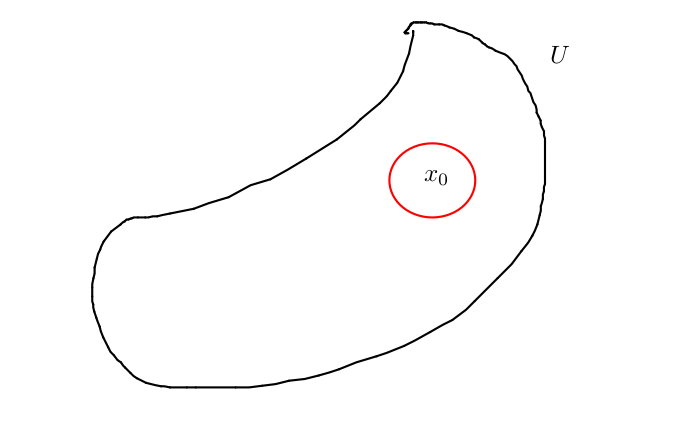
\includegraphics[scale=0.3]{figures/recip_ouvert.png}
      \caption{Illustration}
      \label{}
    \end{figure}

    $J = ]a,b[$.

    $x_0 \in f ^{-1} (J) \implies f(x_0) \in J \implies a \less f(x_0) \less b \implies \exists \varepsilon  \bg 0 \text{ tel que } $

    $$ a \less f(x_0) - \varepsilon \less f(x_0) \less f(x_0) + \varepsilon \less b.$$

    On peut choisir $\varepsilon = \min \{ \frac{b-f(x_0)}{2}, \frac{f(x_0)-a}{2} \} $.

    \begin{figure}[h!]
      \centering
      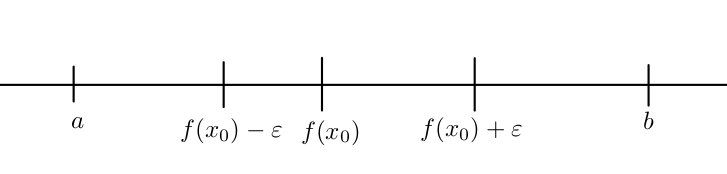
\includegraphics[scale=0.3]{figures/demo_prop_1.png}
      \caption{On choisit $\varepsilon $ de cette sorte}
      \label{}
    \end{figure}

    Donc il y a $\delta \bg 0$ tel que

    \begin{gather*}
      \Vert x-x_0 \Vert \less \delta  \implies \lvert f(x)- f(x_0) \rvert \less \varepsilon \\
      \implies - \varepsilon \less f(x) -f(x_0) \less \varepsilon \\
      \implies f(x_0) - \varepsilon \less f(x) \less f(x_0)+ \varepsilon \implies a \less f(x) \less b \\
      \implies f(x) \in J \implies x \in f ^{-1} (J).
    \end{gather*}

    Choisissons $r := \delta $

    $x \in B(x_0, r) \implies \Vert x-x_0 \Vert \less r=\delta  $.

    On a démontré que avec ce choix de $\delta $ on a $x \in f ^{-1} (J) \implies B(x_0, r) \subset f ^{-1} (J)$.

    \item \emph{Si $f ^{-1} (J)$ ouvert pour tout intervalle $J \subset \mathbb{R}$, alors $f$ est continue.}

    Fixons $x_0 \in U : \varepsilon \bg 0$ est donné.

    On met $J = (f(x_0) - \varepsilon , f(x_0)+ \varepsilon ) \neq \emptyset$.

    Par l'hypothèse, $f ^{-1} (J)$ est ouvert, donc $\exists r \bg 0, B(x_0, r) \subset f ^{-1} (J)$.

    On met $\delta := r$.

    \begin{gather*}
      \Vert x-x_0 \Vert \less \delta \implies x \in B(x_0, \delta ) = B(x_0, r)\\
      \implies x \in f ^{-1} (J) \implies f(x) \in J \\
      \implies f(x_0) - \varepsilon \less f(x) \less f(x_0) + \varepsilon \implies - \varepsilon \less f(x) - f(x_0) \less \varepsilon \\
      \implies \lvert f(x) - f(x_0) \rvert \less \varepsilon .
    \end{gather*}
  \end{enumerate}
\end{proof}

On peut aussi généraliser ces définitions et la proposition aux cas où $f: U \to \mathbb{R}^m$ est une application de $U$ dans $\mathbb{R}^m$, avec

$$ f(x^1, \dots, x^n) = (f_1(x^1, \dots, x^n), \dots, f_m(x^1, \dots, x^m)).$$

\paragraph{Exemple}

$f(x^1, x^2) = ((x^1) ^2+ 3 \cos(x^2) e^{x^1-x^2} )$, $n=2, m=2, U = \mathbb{R}^2$.

\begin{definition}
  $f$ est continue en $x_0 \in U$ si

  $$ \forall \varepsilon  \bg 0, \exists \delta  \bg 0, \forall x \in U, \Vert x-x_0 \Vert \less \delta \implies \Vert f(x)-f(x_0) \Vert \less \varepsilon, $$

  avec   $\Vert f(x)-f(x_0) \Vert = \sqrt{ (f_1(x)-f_1(x_0)) ^2 + \dots + (f_m(x)-f_m(x_0)) ^2 } $.
\end{definition}

\begin{definition}
  $f : U \to \mathbb{R}^m$ est continue quand $f$ est continue en $x, \forall x \in U$.
\end{definition}

\begin{prop} \label{continue}
  Les 3 conditions suivantes sont équivalentes.

  \begin{enumerate}
    \item $f : U \to \mathbb{R}^m$ est continue ;
    \item $\forall j \in \{ 1, \dots, m \} $, $f_j$ est continue ;
    \item $\forall V \subseteq \mathbb{R}^m$ ensemble ouvert, $f  ^{-1} (V)$ est ouvert.
  \end{enumerate}
\end{prop}

\begin{figure}[h!]
  \centering
  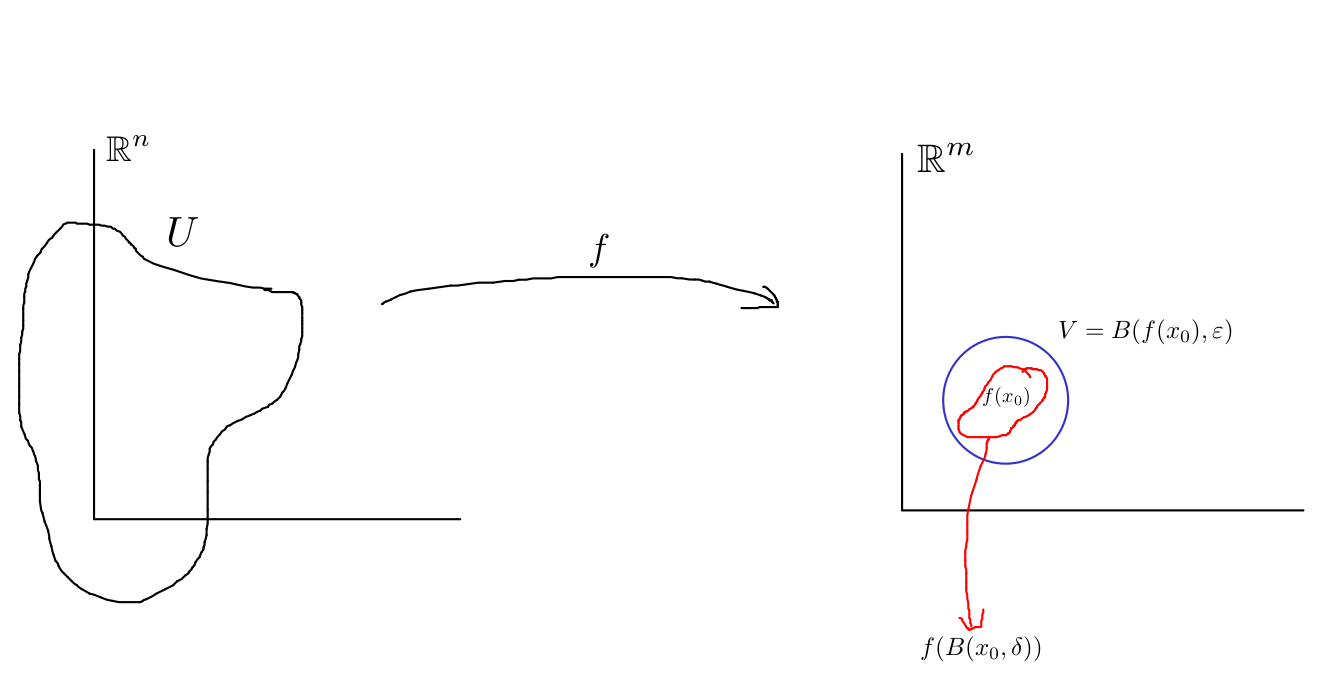
\includegraphics[scale=0.2]{figures/boule_continue.png}
  \caption{Illustration pour \ref{continue}}
  \label{}
\end{figure}



\section{Dérivée, dérivée partielle, différentielle}

$ f : U \to \mathbb{R}$.

$x \in U$ fixé.

La dérivée partielle $\frac{\partial f }{\partial x^i} $, pour $ i \in \{ 1, \dots, n \} $ et $x = (x^1, \dots, x^n)$ est définie par

\begin{gather*}
  \frac{\partial f }{\partial x^i} (x^1, \dots, x^n) := \lim_{h \to 0} \frac{f(x^1, \dots, x^i + h, \dots, x^n)}{h}
\end{gather*}

si la limite existe.

Si $e_i \in \mathbb{R}^n$ est le vecteur $e_i = (0,0,  \dots, 0, \overbrace{1}^{i\text{-ème}}, 0, \dots, 0)$ (tel que $\{ e_1, \dots, e_n \} $ est la base standard de l'espace linéaire $\mathbb{R}^n$), on a

\begin{gather*}
  \frac{\partial f }{\partial x^i }(x) := \lim_{h \to 0} \frac{f(x+h e_i)}{h}  .
\end{gather*}

On peut aussi calculer les dérivées partielles de $\frac{\partial f }{\partial x^i} $. En général, pour tout $k \geq 1$,

\[\frac{\partial ^{k} f }{\partial x^{i_k} \partial x _{i_{k-1}} \dots \partial x^{i_2} \partial x^{i_1}}  = \frac{\partial  }{\partial x^{i_k}} \left(\frac{\partial  }{\partial x _{i_{k-1}}} \dots \left(\frac{\partial f }{\partial x^{i_1}} \right) \right) .\]



$i_1 \in \{ 1, \dots, n \}, \dots, i_k \in \{ 1, \dots, n \} $.

Pour $k=1$, il y a $n$ dérivées partielles.

Pour $k=2, i_1 \longrightarrow$ $n$ choix de $\{ 1, \dots, n \} $.

$i_2 \longrightarrow $ $n$ choix.

Donc il y a $n ^2$ choix.

En général, il y a $n ^{k}$ dérivées partielles différentes de l'ordre $k$.

\begin{definition}
  $r \in \mathbb{N}$.

  On dit que $f : U \to \mathbb{R}$ est une application de classe $\mathcal{C}^r$  ou tout simplement $f$ est $\mathcal{C}^r$ quand

  \begin{enumerate}
    \item Si $r=0$, $f$ est continue.
    \item Si $r \geq 1$, $f$ est continue et les dérivées partielles d'ordre $k$ existent partout dans $U$ et elles sont toutes les applications continues dans $U$ et ceci pour tout $ 1 \leq k \leq r$.
    \item Pour $f : U \to \mathbb{R}^m$, une application, on dit que $f$ est $\mathcal{C}^r$ si $\forall j \in \{ 1, \dots, m \} $, $f_j$ est une application $\mathcal{C}^r$, avec $f = (f_1, \dots, f_m)$.

    On dit que $f$ est $\mathcal{C}^\infty$ quand $\forall r \in \mathbb{N}$, $f$ est $\mathcal{C}^r$.
  \end{enumerate}
\end{definition}

\subsection{Différentiabilité des fonctions multi-variables}

$U \subseteq \mathbb{R}^n$ ouvert, $f : U \to \mathbb{R}^m$, $x=(x^1, \dots, x^n) \in U$, $f = (f_1, \dots, f_m)$.

On dit que $f$ est différentiable à $x \in U$ quand il existe une application linéaire $L : \mathbb{R}^n \to \mathbb{R}^m$ telle que

\begin{gather*}
  \forall \varepsilon \bg 0, \exists \delta  \bg 0 \text{ si } \Vert h \Vert \less \delta \text{ et } x+h \in U, \text{ alors } \Vert f(x+h) - (f(x)+L(h)) \Vert \less \varepsilon \Vert h \Vert .
\end{gather*}

\begin{figure}[h!]
  \centering
  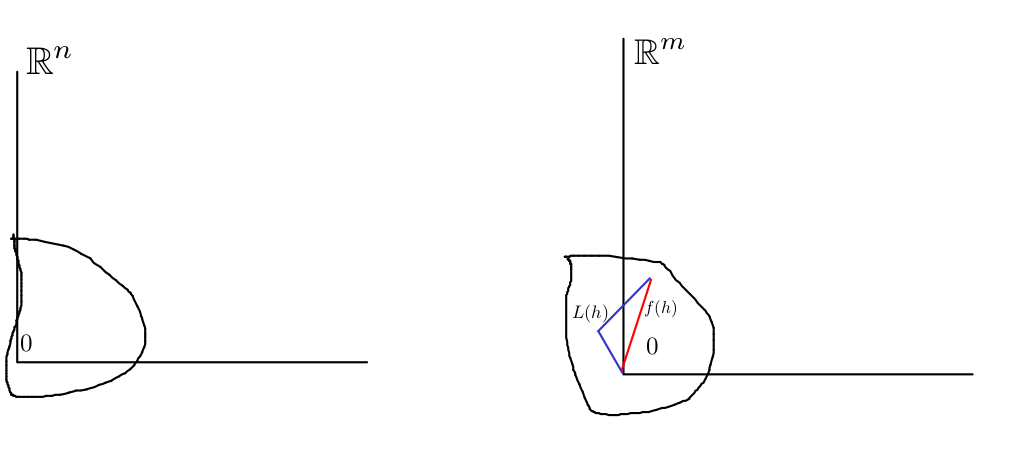
\includegraphics[scale=0.3]{figures/diff.png}
  \caption{Exemple illustratif avec $x=0, f(0) = 0$}
  \label{}
\end{figure}

Cas particulier: $f(0) =0$, $f$ différentiable en 0 si $\forall \varepsilon  \bg 0$, $\exists \delta \bg 0, \Vert h \Vert \less \delta \implies \Vert f(h) - L(h) \Vert \less \varepsilon \Vert h \Vert  $.

\begin{prop}
  $n=1, m=1, f : I \to \mathbb{R}$ est différentiable selon la définition donnée sur un point $x \in I$ si et seulement si $f'(x)$ existe.
\end{prop}

\begin{proof}

  \

  \begin{enumerate}
    \item \emph{Sens direct : $f$ différentiable en $x \in I$ $\implies f'(x)$ existe.}

    $\exists L : \mathbb{R} \to \mathbb{R}$ telle que

    $$ \forall \varepsilon \bg 0, \exists \delta \bg 0, \Vert h \Vert \less \delta , x+h \in I \implies \Vert f(x+h) - f(x) -L(h) \Vert \less \varepsilon \Vert h \Vert.$$

    $L(h) = ah$ pour un $a \in \mathbb{R}$ quelconque mais fixé.

    $a$ est la pente ou le coefficient directeur.

    Prenons $a$   la pente du graphe de $L$ (comme $L$ linéaire, $\exists a \in \mathbb{R}$ tel que $\forall h \in \mathbb{R}, L(h) = ah$).

    On obtient

    $$ \forall \varepsilon \bg 0, \exists \delta \bg 0, \lvert h \rvert \less \delta , x+h \in I \implies \lvert f(x+h) -f(x)-ah \rvert \leq \varepsilon \lvert h \rvert.$$

    On divise par $\lvert h \rvert \neq 0$ pour obtenir

    \begin{gather*}
      \left\lvert \frac{f(x+h)-f(x)}{h} - \frac{ah}{h} \right\rvert \leq \varepsilon.
    \end{gather*}

    \begin{gather*}
      \forall \varepsilon  \bg 0, \exists \delta  \bg 0 \text{ tel que } \lvert h \rvert \less \delta , h+x \in I, \text{ alors } \left\lvert \frac{f(x+h)-f(x)}{h}-a \right\rvert \leq \varepsilon,
    \end{gather*}

    c'est à dire

    \begin{gather*}
      \lim_{h \to 0} \frac{f(x+h)-f(x)}{h} = a.
    \end{gather*}

    Donc $f'(x)$ existe et $f'(x) = a$.

    \item \emph{Sens réciproque : $f'(x)$ existe $\implies f$ différentiable.}

    Si $f'(x)$ existe, on met $a :=f'(x)$.

    On définit $L(h) =ah$. On sait que

    $$ \lim_{h \to 0} \frac{f(x+h)-f(x)}{h} = f'(x) = a.$$

    Donc

    \begin{gather*}
      \forall \varepsilon \bg 0, \exists \delta  \bg 0, \lvert h \rvert \less \delta \implies \left\lvert \frac{f(x+h)-f(x)}{h} -a \right\rvert \leq \varepsilon  \\
      \implies \lvert f(x+h) -f(x) -ah \rvert \leq \varepsilon \lvert h \rvert \\
      \implies \forall h, \lvert h \rvert \less \delta, \text{ on a } \lvert f(x+h) - f(x) -ah \rvert \leq \varepsilon \lvert h \rvert.
    \end{gather*}

    $f$ est différentiable selon notre définition avec $L(h) =ah$.
  \end{enumerate}
\end{proof}


On suppose maintenant que $f:U \to \mathbb{R}^m, U \subseteq \mathbb{R}^n$.

Pour $x \in U$, $f$ différentiable en $x$ si $\exists L : \mathbb{R}^n \to \mathbb{R}^m$ linéaire telle que

\begin{gather*}
  \forall \varepsilon  \bg 0, \exists \delta  \bg 0, \forall h \in \mathbb{R}^n, \Vert h \Vert \less \delta, x+h \in U \implies \Vert f(x+h) -f(x)-L(h) \Vert \leq \varepsilon \Vert h \Vert.
\end{gather*}

On note $\mathscr{L}(\mathbb{R}^n, \mathbb{R}^m) = \{  T: \mathbb{R}^n \to \mathbb{R}^m \mid T \text{ est linéaire }   \} $.

On écrit dans ce cas là que $Df(x) = L \in \mathscr{L}(\mathbb{R}^n, \mathbb{R}^m)  $.

En particulier, si $f$ est différentiable pour tout $x \in U$, on obtient une application $$Df : U \to \mathscr{L}(\mathbb{R}^n, \mathbb{R}^m). $$

\subparagraph{Rappel} Chaque transformation linéaire est uniquement représentée par une matrice au cas où les bases des espaces de départ et d'arrivée sont fixées.

Si on choisit les bases standard $\alpha = \{ e_1, \dots, e_n \} $ pour $ \mathbb{R}^n$ et $ \beta = \{ e_1, \dots, e_m \} \in \mathbb{R}^m $, $T \in \mathscr{L}(\mathbb{R}^n, \mathbb{R}^m) $.

$$ [T] _{\beta } ^{\alpha} := A = [A _{ij}] _{m \times n}$$

et on a $$ T(e_j) = \sum_{i=1}^{m} A _{ij} e_i  = \begin{pmatrix}
  A _{1j} \\
  A _{2j} \\
  \vdots \\
  A _{mj}
\end{pmatrix}.$$

C'est la j-ième colonne de la matrice $A$.

En particulier, pour chaque $x \in U$ où $f$ est différentiable, en fixant les bases standard de $\mathbb{R}^n$ et $\mathbb{R}^m$, on peut supposer que $Df(x) \in \mathbb{R} ^{m \times n}$.

On peut identifier $\mathscr{L}(\mathbb{R}^n, \mathbb{R}^m) $ avec $\mathbb{R} ^{m \times n} = \{ [A _{ij}], 1 \leq i \leq n, 1 \leq j \leq m \mid A _{ij} \in \mathbb{R}\} $.

Avec cette identification, on peut utiliser la norme euclidienne de $\mathbb{R} ^{m \times n}, \Vert A \Vert = \left( \sum_{i=1}^{n} \sum_{j=1}^{m} \lvert A _{ij} \rvert ^2 \right) ^{\frac{1}{2}}  $.

Comme ça on peut parler de continuité et de différentiabilité de l'application $$Df : U \to \mathscr{L}(\mathbb{R}^n, \mathbb{R}^m) \simeq \mathbb{R}^{m\times n}.$$

Ou bien on peut encore identifier $\mathbb{R} ^{m \times n}$ avec $\mathbb{R} ^{mn}$. Alors $Df : U \subseteq \mathbb{R}^n \to \mathbb{R} ^{mn}$.

Donc on peut parler de continuité de $Df $, de derivée de $Df$.

Pour $x \in U, D(Df)(x) \in \mathscr{L}(\mathbb{R}^n, \mathscr{L}(\mathbb{R}^n, \mathbb{R}^m) ) $.

On va noter $D(Df)$ par $D ^2f$. Alors $D ^2 f (x) \in \mathscr{L}(\mathbb{R}^n, \mathscr{L}(\mathbb{R}^n, \mathbb{R}^m) ) = \mathscr{L}(\mathbb{R}^n, \mathbb{R}^{m\times n})  $.

$D ^2 f : U \to \mathscr{L}(\mathbb{R}^n, \mathbb{R} ^{m \times n}) \simeq \mathbb{R} ^{mn ^2} $.

\begin{thm}
  $f : U \to \mathbb{R}^m$ une application donnée et $r \in \mathbb{N}$.

  $f$ est de classe $\mathcal{C}^r$ si et seulement si $D ^{k} f : U \to \mathscr{L}(\mathbb{R}^n, \mathscr{L}(\mathbb{R}^n, \dots) ) \ (\text{de dimension } mn ^{k}) $ existe comme une application pour tout $1 \leq  k \leq r$, et elle est en plus continue.
\end{thm}

\subsection{Deux points fins}

En général, les dérivées partielles de $f$ peuvent exister sans que $Df$ soit définie.

Par exemple, dans $\mathbb{R}^2$, on peut avoir $f$ telle que $\frac{\partial f }{\partial x^1 }(0) $ existe, $\frac{\partial f }{\partial x^2 } $ existe, mais $Df(0)$ n'existe pas.

Par contre, si $Df(x_0)$ existe, alors toutes les dérivées partielles de $f$ existent en $x_0$.

\begin{proof}
  Supposons que $Df(x_0)$ existe. Donc

  $$ \forall \varepsilon \bg 0, \exists \delta \bg 0, \Vert h \Vert \less \delta , x+h \in U  \implies \Vert f(x) -f(x_0) - L(h) \Vert \less \varepsilon \Vert h \Vert . $$

  Fixons une direction $\vec{ v } \in \mathbb{R}^n$ et on met $h = t \vec{ v } $, avec $\Vert \vec{ v }  \Vert \neq 0$. Donc $\Vert h \Vert = \lvert t \rvert \cdot \Vert \vec{ v }  \Vert  $.

  Donc

  \begin{gather*}
    \forall \varepsilon \bg 0, \exists \delta  \bg 0, t \less \frac{\delta }{\Vert \vec{ v }  \Vert}, x_0 + t \vec{ v }  \in U \implies \Vert f(x_0+t \vec{ v } )-f(x_0)-tL(\vec{ v } ) \Vert \less \varepsilon \lvert t \rvert \Vert \vec{ v }  \Vert .
  \end{gather*}

  On pose $\tilde{\varepsilon } = \varepsilon  \Vert \vec{ v }  \Vert \text{ et }  \tilde{\delta } = \frac{\delta }{\Vert \vec{ v }  \Vert } $.

  \begin{gather*}
    \forall \tilde{\varepsilon } \bg 0, \exists \tilde{ \delta } \bg 0 \text{ tel que } \lvert t \rvert \less \tilde{\delta } \implies \Vert f(x_0+t \vec{ v } ) -f(x_0)-tL(\vec{ v } ) \Vert   \leq \tilde{\varepsilon }\lvert t \rvert \\
    \forall \tilde{\varepsilon } \bg 0, \exists \tilde{ \delta } \bg 0,  0 < \lvert t \rvert \less \tilde{\delta } \implies \left\Vert \frac{1}{t}\left(f(x_0 + t \vec{ v } ) -f(x_0)) - L(\vec{ v } \right) \right\Vert \leq \tilde{\varepsilon } \\
    \implies \lim_{t \to 0} \frac{1}{t}\left(f(x_0+t \vec{ v } )-f(x_0)\right) = L(\vec{ v } ) = Df(x_0)(\vec{ v } ) .
  \end{gather*}

  On définit
  \begin{equation*}
    D _{\vec{ v } }f(x_0) := \lim_{t \to 0} \frac{1}{t}(f(x_0+t \vec{ v } )-f(x_0)).
  \end{equation*}

  Donc si $Df(x_0)$ existe, la dérivée directionnelle de $f$ en $x_0$ dans une direction $\vec{ v } \in \mathbb{R}^n$ existe et on a

  $$ D \vec{ v } f(x_0) = Df(x_0)(\vec{ v } ) \in \mathbb{R}^m.$$

  En particulier, si $\vec{ v } = e_j, 1 \leq j \leq n $,
  \begin{equation*}
    \frac{\partial f }{\partial x^j }f(x_0) = D _{e _{j}} f(x_0) = Df(x_0)(e_j).
  \end{equation*}
\end{proof}

Il se peut que toutes les dérivées directionnelles $D _{\vec{ v } }f(x_0)$ existent pour tout $\vec{ v } \in \mathbb{R}^n $ alors que $Df(x_0)$ n'existe pas.

 \begin{thm}
  Si $f : U \to \mathbb{R}^m, x_0 \in U$.

  Si $Df(x_0)$ existe, alors $f$ est continue en $x_0$.
\end{thm}

\begin{proof}
  En exercice.
\end{proof}

Il se peut que toutes les dérivées directionnelles $D _{\vec{ v } } f(x_0)$ existent pour tout $\vec{ v } \in \mathbb{R}^n$ en $x_0 \in U$ sans que pour autant $f$ soit continue en $x_0$.


\begin{exemple}
Soit
$$
f:\mathbb{R}^2 \to \mathbb{R}, \quad f(x,y):= \frac{xy^2}{x^2 + y^6}\quad \mbox{si}\,\, (x,y) \neq 0, \,\, f(0,0):=0.
$$  Alors pour toute $\vec{v}\in \mathbb{R}^2$, $D_{\vec{v}} f(0,0)$ est d\'efinit, mais $f$ n'est m\^eme pas continue \`a $(0,0)$.

\end{exemple}



Si la matrice de $Df(x_0)$ est donnée par $[A _{ij}] _{\substack{1 \leq i \leq n \\ 1 \leq j \leq m}}$.

$$ \forall j \in \{ 1, \dots, n \}, A _{e_j} = \frac{\partial f }{\partial x^j}(x_0) = \left[ \begin{matrix}
  \frac{\partial f_1 }{\partial x^j}(x_0) \\
  \vdots \\
  \frac{\partial f_m }{\partial x^j}(x_0)
\end{matrix} \right].$$

$$ Df = \left[ \begin{matrix}
  \frac{\partial f_1 }{\partial x^1 } & \dots & \frac{\partial f_1 }{\partial x^n }  \\
  \vdots & \ddots & \vdots \\
  \frac{\partial f_m }{\partial x^1 } & \dots & \frac{\partial f_m}{\partial x^n }
\end{matrix} \right].$$

C'est la matrice jacobienne de $f$.

\

\subsection{La dérivée de composition}



$f : \mathbb{R} \to \mathbb{R}$, $g : \mathbb{R} \to \mathbb{R}$, $(g \circ f)'(x) = g'(f(x))f'(x)$.

$f : U \to \mathbb{R}^m$, $g : V \to \mathbb{R}^p$.

Supposons que pour $x_0 \in U$, $f(x_0) \in V$.

\begin{figure}[h!]
  \centering
  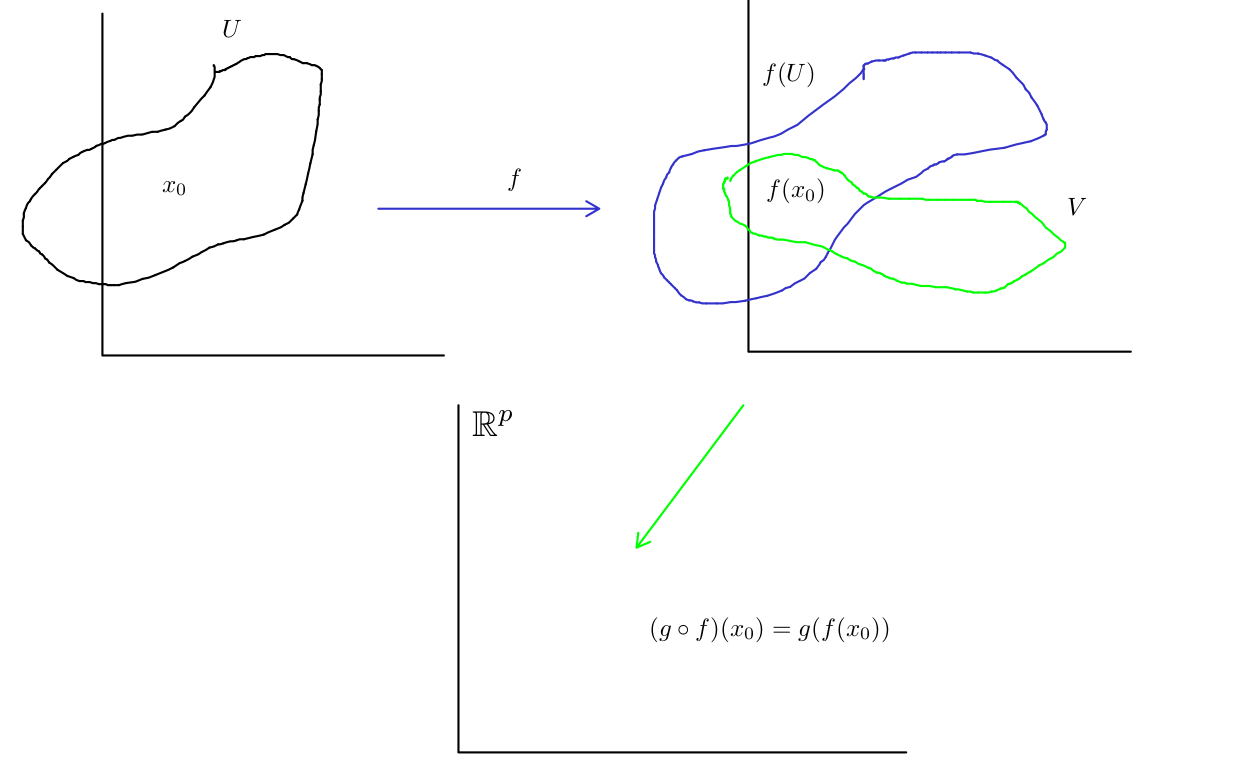
\includegraphics[scale=0.3]{figures/composition.png}
  \caption{La différentiation composée}
  \label{}
\end{figure}

Si $f$ est continue, $g \circ f$ est définie dans un voisinage de $x_0$, par exemple dans une boule ouverte $B(x_0, r) = \widetilde{U} \subset U \cap f ^{-1} (V)$.

$g \circ f : \widetilde{U} \to \mathbb{R}^p$.

Supposons que les trois dérivées $Df(x_0), Dg(f(x_0)), D(g \circ f)(x_0)$ existent.

$Df(x_0) \in \mathscr{L}(\mathbb{R}^n, \mathbb{R}^m) $.

$Dg(f(x_0)) \in \mathscr{L}(\mathbb{R}^m, \mathbb{R}^p) $.

$D(g \circ f) \in \mathscr{L} (\mathbb{R}^n, \mathbb{R}^p)$.

\begin{thm}
  Supposons que $f$ est dérivable en $x_0 \in U$ avec la dérivée $Df(x_0)$ et $g$ est dérivable en $f(x_0) \in V$ avec la dérivée $Dg(f(x_0))$, alors $g \circ f$ est bien dérivable en $x_0 \in U$ et

  $$ D(g \circ f)(x_0) = Dg(f(x_0)) \circ Df(x_0).$$
\end{thm}

Si on utilise les matrices jacobiennes de chaque dérivée ($1 \leq k \leq m, 1 \leq j \leq n, 1 \leq i \leq p$),

\begin{gather*}
  \left[ \frac{\partial (g \circ f)_i }{\partial x^j}  \right]_{p \times n}(x_0) = \left[ \frac{\partial g_i }{\partial y^k }  \right] _{p \times m}(f(x_0))  \times \left[ \frac{\partial f_k }{\partial x^j} \right] _{m \times n}(x_0).
\end{gather*}

\begin{gather*}
  \left[ \frac{\partial z^i }{\partial x^j } \right](x_0) = \left[ \frac{\partial z^i }{\partial y^k } \right](f(x_0)) \times \left[\frac{\partial y^k }{\partial x^j} \right](x_0).
\end{gather*}

On a :

$$ \frac{\partial z^i }{\partial x^j } (x_0) = \sum_{k=1}^{n} \frac{\partial z^i }{\partial y^k}  (f(x_0)) \frac{\partial y^k }{\partial x^j} (x_0). $$




\section{Inversion locale, fonctions implicites, théorème du rang}



\begin{thm}
Supposons que $f : U \to \mathbb{R}^m, U \subseteq \mathbb{R}^n$, $V = f(U)$ est ouvert et $g : V \to \mathbb{R}^n$ est l'inverse de $f$.  Si en plus $f$ et $g$ sont différentiables respectivement \`a $x_0 \in U$ et $f(x_0) \in V$, alors $m=n$ et $Dg(f(x_0)) = (Df(x_0)) ^{-1} $, c'est à dire en particulier $Df(x_0)$ est une transformation linéaire inversible.
\end{thm}

\begin{proof}



\begin{lemma} (exercise)
  Si $L : \mathbb{R}^n \to \mathbb{R}^m$ est une fonction linéaire, $\vec{ b } \in \mathbb{R}^m $ et $T(x) = L(x) + \vec{ b } $, $T : \mathbb{R}^n \to \mathbb{R}^m$.

  Ainsi $T$ est différentiable dans $\mathbb{R}^n$ et

  $$ \forall x \in \mathbb{R}^n, DT(x) = L.$$

Dans ce cas, $DT : \mathbb{R}^n \to \mathscr{L}(\mathbb{R}^n, \mathbb{R}^m) $ est une application constante (les dérivées partielles de $T$ aussi).
\end{lemma}


Comme $g$ est l'inverse de $f$, on a  $g \circ f : U \to \mathbb{R}^n$ et $g \circ f = \operatorname{id} _{U}$, o\`u $\operatorname{id} _{U}$ est l'application d'identit\'e sur $U$
$$
\forall x\in U \quad \operatorname{id} _{U} (x) := x.
$$



  Si $f$ est dérivable en $x \in U$ et $g$ dérivable en $f(x) \in V$,  $\operatorname{id}_U = g \circ f$ dérivable en $x_0$ et

  $$ D \operatorname{id} _{U}(x_0) = Dg(f(x_0)) \circ Df(x_0).$$

  $$ \operatorname{id} _{U}(x) = x \implies D \operatorname{id} _{U}(x_0) = \operatorname{id} _{\mathbb{R}^n}  \in \mathscr{L}(\mathbb{R}^n, \mathbb{R}^n).$$

  Donc  $$ \operatorname{id} _{\mathbb{R}^n} = Dg(f(x_0)) \circ Df(x_0).$$

  Aussi, comme $g$ est linéaire de $f$ on a $f \circ g = \operatorname{id} _{V}$, donc

  $$ \operatorname{id} _{\mathbb{R}^m} = Df(x_0) \circ Dg(f(x_0)).$$

  Donc $Df(x_0) \in \mathscr{L} (\mathbb{R}^n , \mathbb R^m)$ est invertible avec l'inverse $Dg(f(x_0))$.  On se rapp\`ele ce fait de l'alg\`bere lin\'eaire que dans ce cas $m=n$.

\end{proof}



\begin{thm}[d'invariance topologique de dimension, L. E. J. Brouwer]
  Si $U \subseteq \mathbb{R}^n, V \subseteq \mathbb{R}^m$, $h : U \to V$ est un homéomorphisme (i.e.$h$ continue, inversible et d'inverse \textbf{continue} $h ^{-1} : V \to U$), alors $m=n$.
\end{thm}

\subsection{Théorème de l'application inverse}


\begin{thm}[De l'application inverse ou bien {\it de l'inverse locale}]
  $U \subseteq \mathbb{R}^n, x_0 \in U, f : U \to \mathbb{R}^{n}$, $f$ est de classe $\mathcal{C}^1$. Supposons que $Df(x_0) \in \mathscr{L}(\mathbb{R}^n, \mathbb{R}^n) $ est inversible.

  Alors il existe des ensembles ouverts $W \subset U$, $x_0 \in W$ et $V \subseteq \mathbb{R}^n$ tels que $f _{|W} : W \to V$ est inversible. L'inverse $(f _{|W}) ^{-1} : V \to W$ est aussi de classe $\mathcal{C}^1$.
\end{thm}

\begin{figure}[h!]
  \centering
  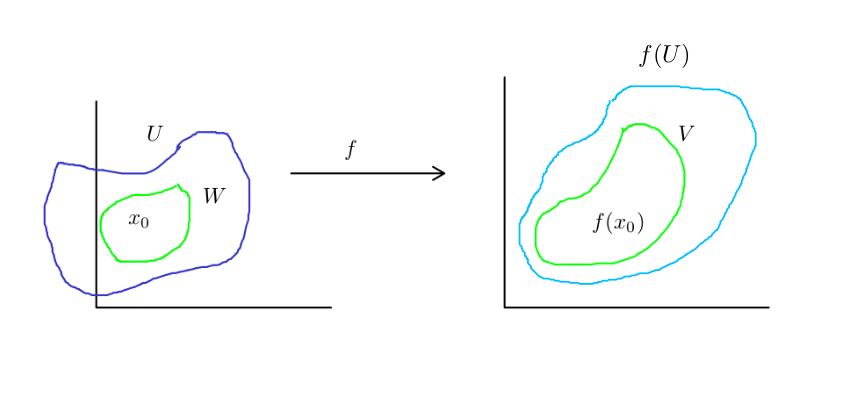
\includegraphics[scale=0.3]{figures/fct_inv_corr.png}
  \caption{Fonctions inversibles}
  \label{}
\end{figure}

\begin{remark}
  Si en plus $f$ est de classe $\mathcal{C}^r$, alors $(f _{|W}) ^{-1} $ est aussi de classe $\mathcal{C}^r$.
\end{remark}

Notons que $\forall y \in V, x \in W, f(x)=y$,

\begin{gather*}
  (D(f _{|W})^{-1} )(y) = (Df(x)) ^{-1}.
\end{gather*}

En particulier, il existe $W$ tel que $Df(x)$ est inversible pour tout $x \in W$.

\subsection{Théorème du rang}\marginnote{20-09-2023}




\begin{thm}[Du rang]
  Soit $f : U \to \mathbb{R}^m$ (avec $U \subset \mathbb{R}^n$ de classe $\mathcal{C}^r, r \geq 1$).  Supposons que $\forall x \in U$,

  \[
  \operatorname{rang}(Df(x)) \equiv k,
  \]

  où $1 \leq k \leq m$ est fixé.

  $(Df(x) : \mathbb{R}^n \to \mathbb{R}^m, \text{ donc } 0 \leq \operatorname{rang}(Df(x)) \leq m)$.

  Soit $x_0 \in U$. Alors il y a des ouverts $W \subseteq \mathbb{R}^n, V \subseteq \mathbb{R}^m \text{ tels que }  x_0 \in W, f(x_0) \in V$ et 2 applications de classe $\mathcal{C}^r$ inversibles

\[
\begin{matrix}
  \varphi : W \to W' \text{ avec } W' \subseteq \mathbb{R}^n \text{ telle que } \varphi(x_0) =0 \\
  \psi : V \to V' \text{ avec } V' \subseteq \mathbb{R}^m \text{ telle que }  \psi(f(x_0)) = 0
\end{matrix}
\]
 telles que $\forall z \in W', z=(z^1, \dots, z^n)$,

  \[
  \psi \circ f \circ \varphi ^{-1} (z^1,z^2, \dots, z^n) = (z^1, z^2, \dots, z^k, 0, \dots, 0).
  \]
\end{thm}

\begin{figure}[h!]
  \centering
  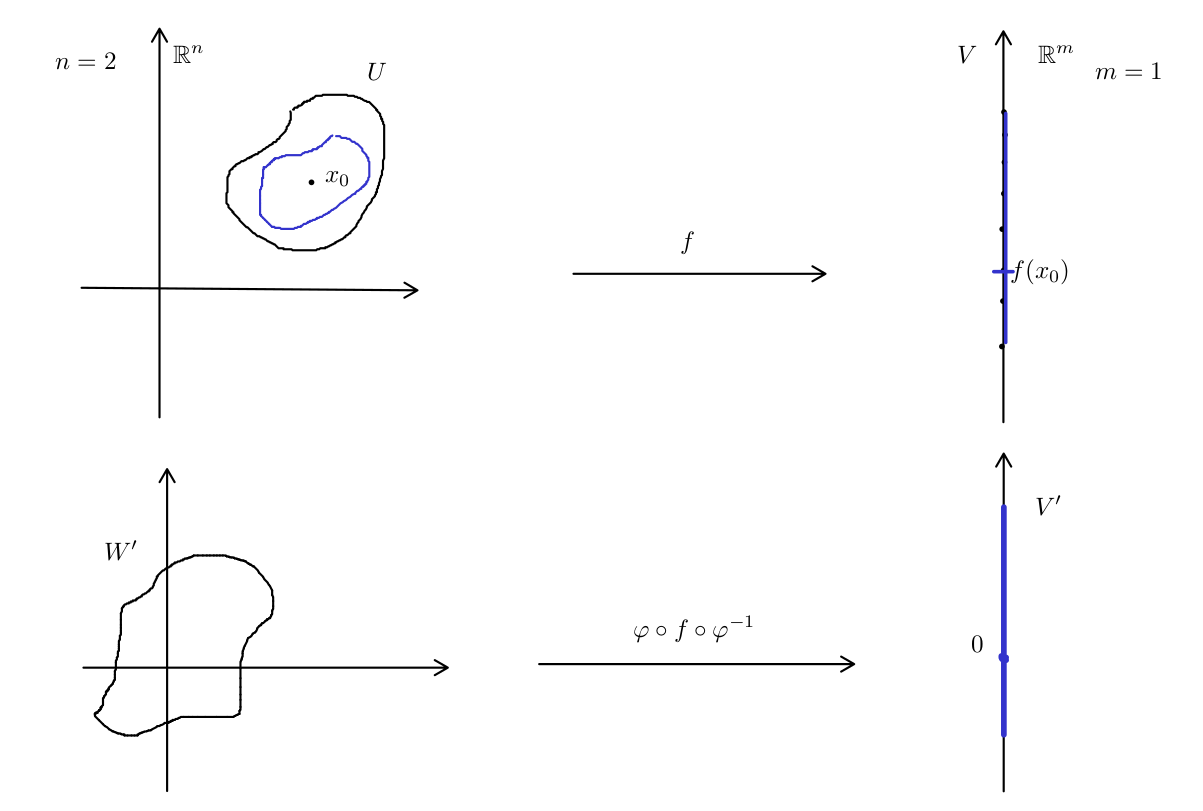
\includegraphics[scale=0.3]{figures/thm-rang-corr.png}
  \caption{Illustration du théorème de rang}
  \label{}
\end{figure}

En particulier, $f(W)$ est un objet de dimension $k$, de régularité $\mathcal{C}^r$ (Si $m=3, k=2, f(W)$ est une surface de classe $\mathcal{C}^r$) et pour tout $y \in f(W), f ^{-1} (y)$ est un objet de dimension $n-k$ de régularité $\mathcal{C}^r$.

On note que les deux applications $\varphi$ et $\psi$ sont de classe $\mathcal{C}^r$ et inversibles. On peut démontrer que dans ce cas-là, les inverses $\varphi ^{-1} $ et $\psi ^{-1} $ sont aussi de classe $\mathcal{C}^r$.

\[
D \varphi ^{-1} (y) = (D \varphi (\varphi ^{-1} (y)))^{-1} , y \in W'.
\]

$\varphi ^{-1} $ étant continue, $D \varphi$ étant continue, l'inverse d'une matrice étant continue tant que $\operatorname{det} \neq 0$, $\varphi$ est de classe $\mathcal{C}^1$ inversible $\implies$  $D \varphi ^{-1} (y)$ d\'epend continuellement en $y$ $\implies$ $\varphi ^{-1} $ est de classe $\mathcal{C}^1$.

\begin{definition}[Difféomorphisme]
  Soient $U, U' \subseteq \mathbb{R}^n$ ouverts.

  Si $\varphi : U \to U'$ est une application de classe $\mathcal{C}^r$, avec l'inverse $\varphi ^{-1} : U' \to U$ de classe $\mathcal{C}^r$, on dit que $\varphi$ est un difféomorphisme de classe $\mathcal{C}^r$.
\end{definition}

\begin{remark}[Le théorème de rang dans le cas spécial où $f$ est linéaire]
  Soit $L : \mathbb{R}^n \to \mathbb{R}^m$, $\operatorname{rang}(L) = k, 0 \leq k \leq m$, alors il existe deux bases $\alpha_n$ et $\beta_m$ pour $\mathbb{R}^n$ et $\mathbb{R}^m$ telles que

  \[
  [L] _{\alpha_n} ^{\beta_m} =  \left[\begin{matrix}
    1 & 0 & \dots & 0 \\
    0 & 1 & \dots & 0 \\
    \vdots & \vdots & \ddots & \vdots \\
    0 & 0 & \dots & 0
  \end{matrix}\right] _{m \times n}.
  \]

  (En exercice).
\end{remark}

\begin{corollary}\label{inj}
  $U \subseteq \mathbb{R}^n, f : U \to \mathbb{R}^m$, $f$ est $\mathcal{C}^r, r \geq 1$.

  Supposons que pour $x_0 \in U$, $Df(x_0)$ est injective. $Df(x_0) \in \mathscr{L}(\mathbb{R}^n, \mathbb{R}^m) $. Alors il existe un voisinage $W$ de $x_0$ tel que $f$ est injective sur $W$.
\end{corollary}

\begin{proof}
  Pour $x \in U,$

  \[
  Df(x) = \left[\begin{matrix}
    \frac{\partial f }{\partial x^1} & \dots & \frac{\partial f }{\partial x^n }
  \end{matrix}\right] _{m \times n}.
  \]

  Si $Df(x_0)$ est injective, $\operatorname{rang}(Df(x_0)) = n \ (m \geq  n)$. On obtient une sous-matrice de $Df(x)$ de taille $n \times n$ inversible.
\end{proof}



\begin{lemma}[D'algèbre linéaire]
  $A \in \mathbb{R} ^{m \times n}$. Alors $\operatorname{rang} A = n$ si et seulement si il existe une sous-matrice $B \in \mathbb{R} ^{n \times n}$ de $A$ telle que $\operatorname{det} B \neq 0$.

  %\[
  %\left[\begin{matrix}
  %  \vec{ v_1 } & \dots & \vec{ v_n }
  %\end{matrix}\right],
  %\]

  %$\vec{ v_j } \in \mathbb{R}^m $.

  (En exercice).
\end{lemma}

Alors sous les hypothèse du corollaire \ref{inj}, $\operatorname{rang}Df(x) \equiv n$ dans un voisinage $W$ de $x_0$, appliquant le théorème du rang

\[
\tilde{f} = \varphi \circ f \circ \varphi ^{-1} (z^1, \dots, z^n) = (z^1, \dots, z^n, 0, \dots, 0)
\]

qui est injectif.

\begin{corollary}
  Les mêmes hypothèses que dans le corollaire \ref{inj}.

  Si $Df(x_0)$ est surjective, alors il existe un voisinage ouvert $V \subseteq f(U)$ de $f(x_0)$ (c'est à dire $f(x_0)$ est un point intérieur de $f(U))$ tel que $f$ est surjective sur $V$.
\end{corollary}

Argument à travers l'observation de l'algèbre linéaire qui dit que si $\operatorname{rang}(A) = m, m \leq n, A \in \mathbb{R}^{m \times n}$, il  y a une sous-matrice $B \in \mathbb{R}^{m\times m}$ tel que $\operatorname{det}(B) \neq 0$.

Théorème de rang : $k=m \leq n$.

Les détails en exercice.

\subsection{Théorème de fonctions implicites}


\begin{thm}[De fonctions implicites]
  $U \subseteq \mathbb{R}^n, V \subseteq \mathbb{R}^m$, $F : U \times V \to \mathbb{R}^m$ une application $\mathcal{C}^r, r \geq 1$.

  $(x_0, y_0) \in U \to V$ donné.

  \[
  DF(x_0, y_0) \in \mathbb{R}^{m \times (m+n)}
  \]

  et

  \[
  DF(x_0, y_0) = \left[\begin{matrix}
    \frac{\partial F }{\partial x^1}(x_0, y_0) & \dots &\frac{\partial F }{\partial x^n } (x_0, y_0) & \mid & \frac{\partial F }{\partial y^1 } (x_0, y_0) & \dots & \frac{\partial F }{\partial y^m } (x_0, y_0)
  \end{matrix}\right] _{m \times (m+n)}.
  \]

  Pour tout $(x_0, y_0) \in U \times V, \, DyF(x_0, y_0) \in \mathbb{R}^{m \times m}$,

  $$
  DyF(x_0, y_0) =  \left[\begin{matrix}
\frac{\partial F }{\partial y^1 } (x_0, y_0) & \dots & \frac{\partial F }{\partial y^m } (x_0, y_0)
  \end{matrix}\right] _{m \times (m)}.
  $$
   Supposons que $DyF(x_0, y_0)$ est inversible. Alors il existe un voisinage $W$ de $x_0$ dans $U$ et une application $\mathcal{C}^r$ $f : W \to V$ telle que $f(x_0) = y_0$ et

  \[
  \forall x \in W, F(x, f(x)) = F(x_0, y_0).
  \]
\end{thm}

\begin{figure}[h!]
  \centering
  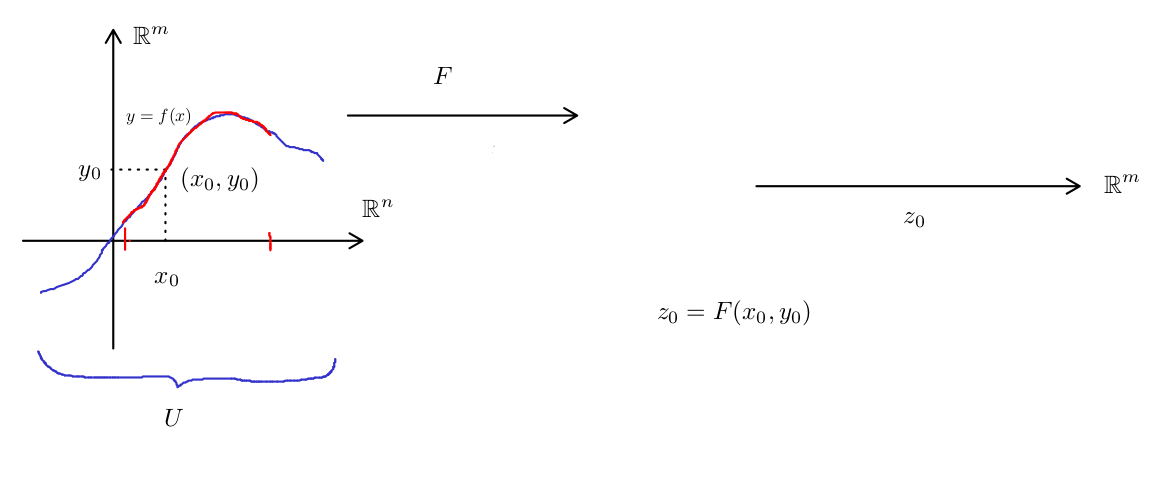
\includegraphics[scale=0.3]{figures/fct_impl.png}
  \caption{Illustration du théorème de fonctions implicites}
  \label{}
\end{figure}

Donc le graphe de $x \longrightarrow f(x)$ dans $W \times V$ pour l'application $f: W \to V$ est à l'intérieur de $F ^{-1} (z^0)$.

On peut dire que la fonction implicite

\[
F(x,y) = z^0, x \in \mathbb{R}^n, y \in \mathbb{R}^m, z^0 \in \mathbb{R}^n
\]

peut être exprimée explicitement par l'application $y = f(x)$ dans un voisinage $W$.

\begin{remark}[Sur le théorème des fonctions implicites]
  En effet, si $W' = f(W) \subset V$, on a

  \[
  (x,y) \in W \times W', F(x,y) = z^0 \iff y=f(x),
  \] et donc $F^{-1}(z^0)$ est caract\'eris\'e par le graphe de $f$ sur $W$.
\end{remark}

\paragraph{Exemple}

$m=1=n$.

Si $F(x, y) = y ^2-x$.

\subparagraph{Exemple 1} $x_0 = 0, y_0 =1 , z^0 =1$.

\[
DF = \left[\begin{matrix}
  \frac{\partial F }{\partial x} & \frac{\partial F }{\partial y }
\end{matrix}\right] = \left[\begin{matrix}
  -1 & 2y
\end{matrix}\right] \in \mathcal{C}^\infty.
\]

\[
DyF = [2y] _{1\times 1}.
\]

\[
DyF(x_0, y_0) = 2 y_0 = 2 \neq 0.
\]

Donc près de $(0, 1) = (x_0, y_0), y= f(x)$ a une solution $\mathcal{C} ^{\infty}$.

Mais si $x_0 = 0, y_0 = 0, z^0 = 0$, $DyF(x_0, y_0)=2y_0=0$ n'est pas inversible. $F$ est $\mathcal{C}^\infty$.

Implicitement, près de $(0, 0)$, on a $y ^2 - x = 0$.

On essaie de trouver $y=f(x)$.

$y ^2 = x \implies y = \pm \sqrt{ x } $.

Mais $\sqrt{\cdot} $ n'est pas définie pour $x \less 0$ près de $x_0 = 0$!

Donc il n'y a pas un moyen d'écrire explicitement $F(x,y) = 0$ près de $(0, 0)$ comme une fonction $\mathcal{C}^\infty$.


\section{Algèbre multilinéaire}

Soit $E$ espace vectoriel sur $\mathbb{R}$ de dimension finie $n$, c'est-à-dire il existe $\beta = \{ \vec{ v_1 }, \dots, \vec{ v_n }   \} $ base telle que

\[
\forall \vec{ v } \in E, \exists ! (\alpha_1, \dots, \alpha_n), \,\, \alpha_i \in \mathbb{R},\,\, \vec{ v } = \sum_{i=1}^{n} \alpha_i \vec{ v_i }.
\]

En particulier, $\beta $ engendre $E$ ($E = \operatorname{span}(\beta) = \langle \beta \rangle $) si $\beta$ est libre.

\subsection{L'espace dual $E ^{*}$}
L'espace dual d'un espace vectoriel $E$ est d\'efini par
\[
E ^{*} = \{ T : E \to \mathbb{R} \text{ linéaire}  \} = \mathscr{L}(E, \mathbb{R}) .
\] Les \'el\'ements de $E^*$ sont parfois appel\'es les co-vecteurs.

\begin{thm}
  On a $\operatorname{dim}(E ^{*}) = \operatorname{dim}(E)$.
\end{thm}

\begin{proof}
  Supposons $\beta = (e_1, \dots, e_n) $ est une base ordonnée de $E$. On définit alors $n$ éléments $(e ^{1}, e ^2, \dots, e ^{n})$, $e ^{j} \in E ^{*}$ de la manière suivante :

  \[
  e ^{j}(e_i) = \delta _{i} ^{j} = \begin{cases}
    1 \text{ si } i=j \\
    0 \text{ sinon. }
  \end{cases}
  \]

  \begin{remark}[Personnelle]
    $e ^{j}$ est l'évaluation du vecteur $\vec{ v } \in E$ en $e_j$.
  \end{remark}

  Donc $\displaystyle e ^j \left(\sum_{i=1}^{n} \alpha_i e_i \right) = \sum_{i=1}^{n} \alpha_i e ^{j}(e_i) = \sum_{i=1}^{n} \alpha_i \delta _{i} ^{j} = \alpha_j  $.

  Donc $\forall j \in \{ 1, \dots, n \}, e ^{j} \in E ^{*} $, $\beta ^{*} = \{ e ^{1}, \dots, e ^{n} \} $. On montre que $\beta ^{*}$ est une base pour $E ^{*}$.

  \begin{enumerate}
    \item $\beta ^{*}$ est libre. Supposons que pour $c_j \in \mathbb{R}$,

    \[
    \sum_{j=1}^{n} c_j e ^{j} = 0 \in E ^{*}.
    \]



    Donc pour tout $i$,
    \begin{gather*}
      \left(\sum_{j=1}^{n} c_j e ^{j} \right) (e_i) = 0 \in \mathbb{R} \text{ et } \\
      \left(\sum_{j=1}^{n} c_j e ^{j} \right) (e_i) = \sum_{j=1}^{n}c_j e ^{j}(e_i) = \sum_{j=1}^{n}c_j \delta_i ^{j} = c_i.
    \end{gather*}

    Donc $\forall i, c_i = 0$.

    \item $\beta ^{*}$ engendre $E ^{*}$. Soit $T \in E ^{*}$. Est-ce qu'il existe $\alpha_1,\dots, \alpha_n$ tel que

    \[
    T = \sum_{j=1}^{n} \alpha_j e ^{j} \ ?
    \]

    Essayons de trouver les $\alpha_j$ en appliquant l'identité desirée en $e_i$.

    \begin{gather*}
      \forall i, T(e_i) = \left( \sum_{j=1}^{n} \alpha_j e_j \right)(e_i) = \sum_{j=1}^{n} \alpha_j e_j(e_i) = \sum_{j=1}^{n} \alpha_j \delta_i ^{j} = \alpha_i.
    \end{gather*}

    Donc pour $T \in E ^{*}$ donnée, le candidat pour $\alpha_i$ est

    \[
    \forall i \in \{ 1, \dots, n \}, \alpha_i = T(e_i) \in \mathbb{R},
    \]

    et on obtient que

    \[
    \forall i \in \{ 1, \dots, n \}, T(e_i) = \underbrace{\left(\sum_{j=1}^{n} \alpha_j e ^{j} \right)}_{\tilde {T}}  (e_i).
    \]

    Comme $T$ et $\tilde{T}$ ont les mêmes valeurs sur la base $\beta $, donc $T = \tilde{T}$.

    \[
    T = \sum_{j=1}^{n} T(e_j) e ^{j}.
    \]

  \end{enumerate}
\end{proof}


\begin{definition}
  On dit que $\beta ^{*}$ est la base duale de $\beta $.
\end{definition}

\subsubsection{Le bi-dual}

On considère le dual du dual (le bi-dual) $E ^{**} = (E ^{*}) ^{*}$.


\begin{thm}
  Si $\operatorname{dim}(E) \less \infty$, il y a un isomorphisme canonique entre $E$ et $E ^{**}$.
\end{thm}

On peut définir $E \to E ^{**}$. On pose $e : E \to E ^{**}$.

\[
(\iota(\vec{ v } ))(T) = T(\vec{ v } ),
\]

$\forall T \in E ^{*} = \mathscr{L}(E, \mathbb{R}) $.

\begin{exo}

  \

  \begin{enumerate}
    \item Montrer que $\forall v \in E, \iota(\vec{ v } ) : E ^{*} \to \mathbb{R}$ est une transformation linéaire (et donc
    $\iota(\vec{ v } )  \in E^{**}$).
    \item Montrer que $\iota : E \to E ^{**}$ est une transformation linéaire.
    \item Montrer que $\iota$ est bijective (donc un isomorphisme).
  \end{enumerate}
\end{exo}

\begin{proof}

  \

  \begin{enumerate}
    \item \begin{gather*}
      \iota(\vec{ v } ) (\alpha T+ S) = (\alpha T+S)(\vec{ v } ) = \alpha T(\vec{ v } )+ S(\vec{ v } ) = \alpha \iota(\vec{ v } )(T)+ \iota(\vec{ v } )(S).
  \end{gather*}
    \item $\iota : E \to E ^{**}$ est linéaire.

    \begin{gather*}
      \iota(\alpha \vec{ v } + \vec{ w }  )(T) = T(\alpha \vec{ v } + \vec{ w } ) \stackrel{T \text{ linéaire} }{=} \alpha T(\vec{ v } )+ T(\vec{ w } ) \\
      = \alpha \iota(\vec{ v } )(T)+ \iota(\vec{ w } ) (T) = ( \alpha \iota (\vec{ v } )+ \iota(\vec{ w }) )(T).
    \end{gather*}

    Comme c'est vrai $\forall T \in E ^{*}$, on a l'identification $\iota(\alpha \vec{ v }+ \vec{ w }  ) = \alpha \iota(\vec{ v } )+ \iota(\vec{ w } )$ (comme un élément de $E ^{**}$). Donc $\iota$ est une transformation linéaire.

    \item On sait que $dim E = dim E ^{*} = dim E ^{**}$ (ce qui veut dire que $\iota$ est surjective). Pour démontrer que $\iota$ est un isomorphisme, il suffit de démontrer que $\operatorname{Ker}(\iota) = \{ 0 \} $ (que $\iota$ est injective).
\medskip

    Si $\vec{ v }  \in \operatorname{Ker}(\iota)$, alors $\iota(\vec{ v } ) = 0 \implies \forall T \in E ^{*}, T(\vec{ v } ) = \iota(\vec{ v })(T) = 0(T) =0$, donc $\vec{ v } $ est tel que $\forall T \in E ^{*}, T(\vec{ v } ) =0$.



    Si $\vec{ v } \neq \vec{ 0 }  $, on peut compléter $\vec{ v } $ avec une base $\{ \vec{ v }, \vec{ v_2 },\dots, \vec{ v_n } \} $ de $E$ et définir $T(\alpha_1 \vec{ v } + \alpha_2 \vec{ v_2 } + \dots + \alpha_n \vec{ v_n }  ) = \alpha_1$. Dans ce cas-là, $T(\vec{ v } ) = 1 \neq 0$.
Ceci est en contradiction avec ce qu'on a d\'emontr\'e. Donc $\vec{v} =0$, ce qui d\'emontre  $\operatorname{Ker}(\iota) = \{ 0 \} $.

\bigskip
    Si $\beta = (e_1, \dots, e_n)$ base de $E$. On a vu que la base duale $\beta ^{*} = (e ^{1}, e ^2, \dots, e ^{n})$ est une base de $E ^{*}$.

    \[
    e ^{j}(e_i) = \delta_i ^{j}.
    \]

    \[
    (\beta ^{*}) ^{*} = \beta ^{**} = (\epsilon_1, \epsilon_2, \dots, \epsilon_n).
    \]

    \begin{equation} \label{base1}
      \forall i, \epsilon_i \in E ^{**}, \epsilon_i(e ^{i}) = \delta_i ^{j}, \forall i, j.
    \end{equation}

    On va aussi calculer

    \begin{equation} \label{base2}
      \iota(e_i)(e ^{j}) = e ^{j}(e_i) = \delta_i ^{j}.
    \end{equation}

    $\forall e ^{j}$ de base $\beta ^{*}$, on a

    \[
    \epsilon_i(e ^{j}) = \iota(e_i)(e ^{j}), \quad \epsilon_i, \iota(e_i) \in E ^{**} = \mathscr{L}(E ^{*}, \mathbb{R}).
    \]

    $\epsilon _i$ et $\iota(e_i)$ coincident sur une base de $E ^{*}$, donc

    \[
    \forall i, \epsilon_i = \iota(e_i).
    \]

    Pour simplifier, parfois on identifie $E$ et $E ^{**}$ par l'application $\iota$, c'est-à-dire on met $\vec{ v } = \iota(\vec{ v })$.
  \end{enumerate}
\end{proof}

Les éléments de $E ^{*}$ sont appelés \textbf{les vecteurs covariants}. Les éléments de $E ^{**}$ sont appelés \textbf{les vecteurs contravariants}.

\subsection{Les applications multilinéaires ({\it tenseurs})}

\begin{definition}[Applciations $k$-lin\'eaires]
Supposons que $E_1, E_2, \dots, E_k$, $E'$ sont des espaces vectoriels sur $\mathbb{R}$.

\[
\alpha : E_1 \times E_2 \times \dots \times E_k \longrightarrow E', \quad (\vec{ v_i } \in E_i , \,\, 1 \leq i \leq k,\quad  \alpha(\vec{ v_1 }, \vec{ v_2 }, \dots, \vec{ v_k }) \in E'),
\]

est une application $k$-linéaire quand $\alpha$ est linéaire par rapport à chaque coordonnée dans l'un des espaces $E_i$ quand les autres coordonnées (composantes) sont fixées.

C.\`a.d.  $\alpha$ est $k$-linéaire si $\forall i \in \{ 1, \dots, k \}$, $a \in \mathbb{R}, \forall \vec{ v_i } \in E_i, \vec{ w } \in E_i $, on a

\[
\alpha(\vec{ v_1 }, \vec{ v_2 }, \dots, a \vec{ v_i }+ \vec{ w }, \dots, \vec{ v_k }) = a \alpha(\vec{ v_1 }, \dots, \vec{ v_i }, \dots, \vec{ v_k })+ \alpha(\vec{ v_1 }, \vec{ v_2 }, \dots, \overbrace{\vec{ w } }^{i\text{-ème}}, \dots, \vec{ v_k }).
\]

\end{definition}

\begin{figure}[h!]
  \centering
  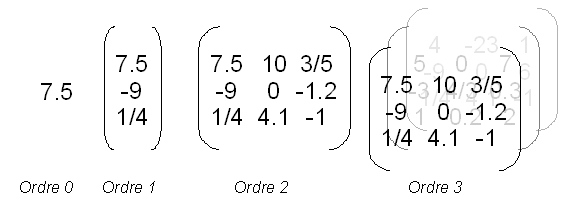
\includegraphics[scale=0.5]{figures/Tensor-order-comparison.png}
  \caption{Représentation des tenseurs dans une base. Les scalaires et les vecteurs constituent des exemples simples de tenseurs. Dans une base donnée, un vecteur (tenseur d'ordre 1) peut être représenté par la donnée d'un \(n\)-uplet de coordonnées. Les matrices \(n \times n\) --- qui peuvent représenter suivant les cas des endomorphismes, des bivecteurs ou encore des formes bilinéaires --- forment une extension des \(n\)-uplets similaire à l'extension que représente les \(n\)-uplets par rapport aux scalaires. Les objets descriptibles par des matrices constituent donc les premiers types de tenseurs non triviaux, appelés tenseurs d'ordre 2. En prolongeant la réflexion on peut imaginer, toujours de manière informelle, des matrices cubiques \(n \times n \times n\), correspondant aux tenseurs d'ordre 3, et ainsi de suite (Wikipédia).}
  \label{}
\end{figure}
\paragraph{Exemples}

\begin{enumerate}
  \item $f(x,y) = xy$, $f : \stackrel{E_1}{\mathbb{R}} \times \stackrel{E_2}{\mathbb{R}} \to \stackrel{E'}{\mathbb{R}}$.
  \item $E_1 = E_2 = \mathbb{R}^n$, $E' = \mathbb{R}$,

  \[
  \alpha(\vec{ v_1 }, \vec{ v_2 } ) = \vec{ v_1 }\cdot \vec{ v_2 }\quad  \text{ 2-linéaire. }
  \]

  \item $E_1 = E_2 = E_3 \equiv \mathbb{R}^3$, $E' = \mathbb{R}$.
  \[
  \alpha(\vec{ v_1 }, \vec{ v_2 }, \vec{ v_3 }) = \vec{ v_1 } \cdot (\vec{ v_2 } \wedge \vec{ v_3 }  ) = det \left( \left[\begin{matrix}
  \vec{ v_1 } \\
  \vec{ v_2 }  \\
  \vec{ v_3 }
  \end{matrix}\right]\right)  _{3 \times 3}.
  \]

  Cette application est 3-linéaire.

  \item $E_1 = E_2 = \dots = E_n = \mathbb{R}^n$.

  \[
  \alpha(\vec{ v_1 }, \vec{ v_2 }, \dots, \vec{ v_n } ) = det \left(\left[\begin{matrix}
  \vec{ v_1 } \\
  \vec{ v_2 } \\
  \vdots \\
  \vec{ v_n }
  \end{matrix}\right]\right).
  \]

  C'est une application $n$-linéaire.

  \item Le déterminant d'une matrice de taille $n \times n$ est une application $n$-linéaire par rapport \`a ses colonnes ou bien par rapport \`a ses lignes.
\end{enumerate}




\subsubsection{Quelques notations}

$E$ espace vectoriel de dimension finie.

On note $\Omega ^{k}(E) := \{ \alpha : \underbrace{E \times E \times \dots \times E}_{k \text{ fois} }  \to \mathbb{R} \mid \alpha \text{ est } k \text{-linéaire}  \} $.

Remarquons que $\Omega ^{1}(E) = \{ \alpha : E \to \mathbb{R} \mid \alpha \text{ est linéaire}  \} = E ^{*}$.

\begin{prop}
  $\forall k \in \mathbb{N} ^{*}, \Omega ^{k}(E) $ est un espace vectoriel de dimension $n ^{k}$.
\end{prop}

\begin{proof}
  Si $\alpha, \beta \in \Omega ^{k}(E), a \in \mathbb{R}$. Pour montrer que \(\Omega ^{k}(E)\) est un espace vectoriel de dimension \(n ^{k}\), on doit montrer deux choses :

  \begin{enumerate}
    \item \(\Omega ^{k}(E)\) est stable par les opérations + et \(\cdot\) (produit par un scalaire).
    \item Il existe une base de cet espace contenant \(n ^{k}\) éléments.
  \end{enumerate}

   Il faut démontrer que $a \alpha+ \beta$ est aussi une application $k$-linéaire sur $E ^k = \overbrace{E \times \dots \times E}^{k \text{ fois}}$.

  \begin{gather*}
    (a \alpha + \beta)(b \vec{ v_1 }+ \vec{ w }, \dots) = a[\alpha(b \vec{ v_1 }+ \vec{ w }, \dots)]+ \beta(b \vec{ v_1 }+\vec{ w })\\
    = a[b \alpha(\vec{ v_1 }, \dots)+ \alpha(\vec{ w }, \dots)] + b \beta(v_1, \dots) + \beta(\vec{ w }, \dots) \\
    = b[a \alpha+ \beta](\vec{ v_1 }, \dots )+ [a \alpha+ \beta](\vec{ w }, \dots)
  \end{gather*}

  De même pour chaque $1 \leq i \leq k$.

  Pour trouver la dimension de $\Omega ^{k}(E)$, il faudra trouver une base de $\Omega ^{k}(E)$. Pour cela, il faudra d'abord introduire ``le produit tensoriel''.
\end{proof}

\begin{definition}[Produit tensoriel]
  Supposons que $\alpha : E_1 \times \dots \times E_k \to \mathbb{R}$ $k$-linéaire, $\beta: E_1' \times \dots \times E_l' \to \mathbb{R}$ $l$-linéaire.

  On définit

  \[
  \alpha \otimes \beta : E_1 \times \dots \times E_k \times E_1' \times \dots \times E_l' \longrightarrow \mathbb{R}
  \]

  telle que

  \[
  \alpha \otimes \beta(\vec{ v_1 }, \dots, \vec{ v_k }, \vec{ v_1' }, \dots, \vec{ v_l'} ):=\alpha(\vec{ v_1 }, \dots, \vec{ v_k }) \beta(\vec{ v_1' }, \dots, \vec{ v_l'})
  \]

  qui est une application $(k+l)$-linéaire (avec $\vec{ v_i } \in E_i, i \in \{ 1, \dots, k \}, \vec{ v_j' } \in E_j', j \in \{ 1, \dots, l\}$).
\end{definition}

Les applications $k$-linéaires sont appelées les tenseurs covariants d'ordre $k$.

\begin{exo}
  On montre que $\otimes$ est une opération associative.

  $\forall \alpha, \beta, \gamma $ tenseurs covariants,

  \[
  (\alpha \otimes \beta) \otimes \gamma = \alpha \otimes (\beta \otimes \gamma ).
  \]
\end{exo}

\paragraph{Exemple}
$~$ \\ $E_1 = \mathbb{R}^{n}, E_1' = \mathbb{R} ^{n}, k=l=1, \\ \alpha \in E_1 ^{*}, \alpha(\vec{ v }) =2 \vec{ v } \cdot e_1  , \forall \vec{ v } \in \mathbb{R}^n, \\ \beta \in E_1^{'*}, \beta (\vec{ v' } ) = \vec{ v' } \cdot e_1, \forall \vec{ v' } \in \mathbb{R}^n$.

\[
\alpha \otimes \beta(\vec{v}, \vec{ w }) = 2 (\vec{ v }\cdot e_1)(\vec{ w } \cdot e_1)
\]

et

\[
\beta \otimes \alpha(\vec{ v}, \vec{ w } ) = 2(\vec{ w }\cdot e_1 )  (\vec{ v } \cdot e_1 ).
\]

Mais si $\tilde{\beta}(\vec{ v' } ) = \vec{ v' } \cdot e_2 $,

\begin{gather*}
  \alpha \otimes \tilde{\beta} (\vec{ v }, \vec{ w }) = 2 (\vec{ v } \cdot e_1 )(\vec{ w }\cdot e_2 ), \\
  \text{mais } \tilde{\beta }\otimes \alpha(\vec{ v }, \vec{ w }  ) = 2   (\vec{ w }\cdot e_1 ) (\vec{ v }\cdot e_2 ).
\end{gather*}

Le produit tensoriel n'est donc pas commutatif.

\

$E ^{k} = \underbrace{E \times \dots \times E}_{k \text{ fois} }$

$\Omega ^{k}(E) := \{ \alpha : \underbrace{E \times E \times \dots \times E}_{k \text{ fois} }  \to \mathbb{R} \mid \alpha \text{ est } k \text{-linéaire}  \} $.

\begin{prop}\label{dim-tens}
  $\Omega ^{k}(E)$ est un espace vectoriel de dimension $n ^k$, où $n = dim(E)$.
\end{prop}

\begin{proof}
  On rappelle que $\operatorname{dim}(E) = n$, que $(e_1, \dots, e_n)$ est une base de $E$ et que $(e ^{1}, \dots, e ^{n})$ est une base de $E ^{*} = \Omega ^{1}(E)$.

  Par exemple si on prend

  \[
  \underbrace{e^{1} \otimes e ^{1} \otimes \dots \otimes e ^{1}}_{k \text{ fois} } : E \times \dots \times E \to \mathbb{R},
  \]

  on aura alors

  \begin{gather*}
    e^{1} \otimes e ^{1} \otimes \dots \otimes e ^{1}(\vec{ v_1 }, \dots, \vec{ v_n }  ), \vec{ v_i } \in E, \\
    = e ^{1}(\vec{ v_1 } ) e ^{1}(\vec{ v_2 } ) \dots e ^{1}(\vec{ v_n }).
  \end{gather*}

  Posons $\mathscr{A} = \{ e ^{i_1} \otimes e ^{i_2} \otimes \dots \otimes e ^{i_k} \mid \text{pour } 1 \leq j \leq k, 1 \leq i_j \leq n  \} $.

  Il y a $n$ choix pour chaque $e ^{i_j}$ (parmi les \(n\) vecteurs de la base de \(E\)), et il y a \(k\) fois qu'on doit faire ce choix pour $1\le j\le k$, alors, au total, on a $n^k$ choix pour les éléments de $\mathscr{A}$  , ce qui démontre la proposition \ref{dim-tens}. Il nous reste maintenant à montrer que :

  \begin{enumerate}
    \item[(a)] $\mathscr{A} $ engendre $\Omega ^{k}(E)$ ;
    \item[(b)] $\mathscr{A} $ est libre.
  \end{enumerate}

  Soit $\alpha \in \Omega ^{k}(E)$.

  On va démontrer que

  \[
  \alpha \stackrel{?}{=} \sum_{1 \leq i_1, \dots, i_k \leq n}^{} \alpha(e _{i_1}, e _{i_2}, \dots, e _{i_k}) e ^{i_1} \otimes e ^{i_2} \otimes \dots \otimes e ^{i_k}.
  \]

  Prenons $(\vec{ v_1 }, \vec{ v_2 }, \dots, \vec{ v_n }) \in E ^{k}$. On a

  \begin{gather*}
    \vec{ v_j } = \sum_{i=1}^{n} c _{ij} e_i.
  \end{gather*}

  \begin{gather*}
    \alpha(\vec{ v_1 }, \dots, \vec{ v_k }) = \alpha\left(\sum_{i=1}^{n}c _{i1}e_i, \dots, \sum_{i=1}^{n} c _{ik} e_i\right) \\
    = \sum_{i=1}^{n} c _{i1} \alpha\left(e_i, \sum_{i_2}^{} c _{i_2 2} e _{_2 i}, \dots  \right)  \\
    = \sum_{i_1 =1}^{n} \sum_{i_2=1}^{n} \dots \sum_{i_k=1}^{n} c _{i_1 1} c _{i_2 2} \dots c _{i_k k} \alpha(e _{i_1},\dots, e _{i_k}).
  \end{gather*}

  Maintenant, pour

  \[
  \beta = \sum_{1 \leq i_1, \dots, i_k \leq n}^{} \alpha(e_{i_1}, \dots,  e_{i_k}) e ^{i_1}\otimes \dots \otimes e ^{i_k},
  \]

  on calcule pour $\beta  \in \Omega ^{k}(E)$,

  \begin{gather*}
    \beta (\vec{ v_1 }, \dots, \vec{ v_k })= \sum_{i_1}^{} \sum_{i_2}^{} \dots \sum_{i_k}^{} c _{i_1 1} c _{i_2 2} \dots c _{i_k k} \beta(e _{i_1}, \dots, e _{i_k}).
  \end{gather*}

  Mais

  \begin{gather*}
    \beta (e _{i_1}, \dots, e _{i_k}) = \sum_{1 \leq i_1', \dots, i_k' \leq n}^{} \alpha( e _{i_1'}, e _{i_2'}, \dots, e _{i_k'}) e ^{i_1'}\otimes e ^{i_2'} \otimes \dots \otimes e ^{i_k'} (e_{i_1},\dots, e_{i_k}) \\
    = \sum_{1 \leq i_1' \leq \dots \leq i_k' \leq n}^{} \alpha(e _{i_1'}, \dots, e _{i_k'}) e ^{i_1'}(e _{i_1}) e ^{i_2'}(e _{i_2}) \dots e ^{i_k'} (e _{i_k}) \\
    =\sum_{1 \leq i_1', \dots, i_k' \leq n}^{} \alpha(e _{i_1'}, \dots, e _{i_k'}) \delta _{i_1} ^{i_1'} \dots \delta _{i_k} ^{i_k'} = \alpha(e _{i_1}, \dots, e _{i_k}).
  \end{gather*}

  Donc

  \begin{gather*}
  \begin{aligned}
    \beta (\vec{ v_1 }, \dots, \vec{ v_k }  ) & = \sum_{i_1}^{} \sum_{i_2}^{} \dots \sum_{i_k}^{} c _{i_1 1} c _{i_2 2} \dots c _{i_k k} \beta(e _{i_1}, \dots, e _{ik})   \\ &  = \sum_{i_1}^{} \sum_{i_2}^{} \dots \sum_{i_k}^{} c _{i_1 1} c _{i_2 2} \dots c _{i_k k} \alpha(e _{i_1}, \dots, e _{ik}) \\ & =\alpha(\vec{ v_1 }, \dots, \vec{ v_k }  )   .
\end{aligned}
  \end{gather*}

  Donc (a) est démontré, comme $\alpha = \beta$ et $\beta \in span(\mathscr{A} ) = \langle \mathscr{A} \rangle $, où $\mathscr{A} = \{ e ^{i_1} \otimes \dots \otimes e ^{i_k}\} $.

  \

  Montrons que $\mathscr{A} $ est libre. Soit

  \begin{gather*}
    \sum_{1 \leq i_1 , \dots, i_k \leq n}^{} c _{i_1 i_2 \dots i_k}  e ^{i_1} \otimes \dots \otimes e ^{i_k} = 0 \in \Omega ^{k}(E).
  \end{gather*}

  Le même calcul qu'auparavant démontre que

  \[
  0 = 0(e _{i_1}, \dots, e _{i_k}) = c _{i_1 \dots i_k}, \forall i_1, \dots, i_k,
  \]

  donc

  \[
  \forall i_1, \dots, i_k, c _{i_1 \dots i_k} =0,
  \]

  donc $\mathscr{A} $ est libre.
\end{proof}

\begin{remark}
  Si $f : U \to \mathbb{R}^m, U \subseteq \mathbb{R}^n$, $Df(x) \in \mathscr{L}(\mathbb{R}^n, \mathbb{R}^m) $,

  \begin{gather*}
    Df:U \to \mathscr{L}(\mathbb{R}^n, \mathbb{R}^n) \\
    D ^2 f(x) \in \mathscr{L}(\mathbb{R}^n, \mathscr{L}(\mathbb{R}^n, \mathbb{R}^m) ) \\
    \vdots \\
    D ^{n}f(x) \in \mathscr{L}(\mathbb{R}^n, \mathscr{L}(\mathbb{R}^n, \dots, \mathscr{L}(\mathbb{R}^n, \mathbb{R}^m) ) ) .
  \end{gather*}
\end{remark}

\begin{lemma}
  $\mathscr{L}(\mathbb{R}^n, \mathscr{L}(\mathbb{R}^n, \mathbb{R}^m) ) \simeq \{ \alpha : \mathbb{R}^n \times \mathbb{R}^n \to \mathbb{R}^m \mid \alpha \text{ est 2-linéaire} \}  = (\Omega^2(\R^n))^m $.
\end{lemma}
\begin{proof}


Pour un élément $g \in \mathscr{L}(\mathbb{R}^n, \mathscr{L}(\mathbb{R}^n, \mathbb{R}^m) ) $ et $\vec{ v } \in \mathbb{R}^n, g(\vec{ v } ) \in \mathscr{L}(\mathbb{R}^n, \mathbb{R}^m) $.

 On définit

\[
\alpha_g(\vec{ v }, \vec{ w } )  := g(\vec{ v }) ( \vec{ w } )  \in \mathbb{R}^m.
\]

On voit que $\alpha _{g}$ est une application 2-linéaire.

Supposons que $\alpha_g = \alpha _{g'}, $ donc $ \forall \vec{ v }, \vec{ w } \in \mathbb{R}^n, \alpha _{g}(\vec{ v }, \vec{ w }) = \alpha _{g'}(\vec{ v }, \vec{ w }) $, donc $g(\vec{ v } )(\vec{ w } ) = g'(\vec{ v } )(\vec{ w } )$. Donc $\forall \vec{ v } \in \mathbb{R}^n, g(\vec{ v } ) = g'(\vec{ v } ) \in \mathscr{L}(\mathbb{R}^n, \mathbb{R}^m)$, donc $g = g'$. On en déduit que $g \longrightarrow \alpha_g$ est injective. $g\to \alpha_g$ est lin\'eaire, et un argument de dimension peut finir la d\'emonstration.  On peut aussi trouver l'inverse de cette transformation lin\'eaire:

Supposons que $\alpha : \R^n \times \R^n \to \R^m$ est 2-in\'eaire. On d\'efinit
$$
\forall \vec{ v }, \vec{ w }   \in \R^n, \quad g_\alpha (\vec{ v } ) (\vec{ w })  := \alpha(\vec{ v } ,\vec{ w } ).
$$  Pour tout $\vec{ v } \in \R^n$, $g_\alpha (\vec{ v } )$ est une application lin\'eaire de $\R^n$ \`a valeur dans $\R^m$ comme $\alpha$ est lin\'eaire en $\vec{ w}$, donc $g(\vec{ v } ) \in \mathscr{L}(\R^n, \R^m)$.  Comme $\alpha$
est  est lin\'eaire en $\vec{ v}$,  on obtient que $g_\alpha$ est lin\'eaire, et donc $g_\alpha \in \mathscr{L}(\mathbb{R}^n, \mathscr{L}(\mathbb{R}^n, \mathbb{R}^m))$.

Notez que l'application $g\to \alpha_g$  et son inverse $ \alpha\to g_\alpha$ sont lin\'eaires.
\end{proof}
Par recurrence on peut d\'emontrer que

\begin{lemma}
$\mathscr{L}(\mathbb{R}^n, \mathscr{L}(\mathbb{R}^n, \dots, \mathscr{L}(\mathbb{R}^n, \mathbb{R}^m) ) )
\simeq (\Omega^k(\R^n))^m $.
\end{lemma}

Conclusion: Pour tout $k \in \mathbb N$, $x \in U$, $D ^{k}f(x) \in (\Omega ^{k}(\mathbb{R}^n))^{m}$. Cet espace est de dimension $mn ^{k}$.


\begin{exemple}\marginnote{27-09-2023}
  \(T : \mathbb{R}^2 \to \mathbb{R}, Tx =  2x^1+ 5x^2 \). On définit \(\alpha : \mathbb{R}^2 \times \mathbb{R}^2 \to \mathbb{R}\), \(\alpha((x^1, x^2), (y^1, y^2)) = x^1 y^2-x^2 y^1, \alpha \in \Omega ^2(\mathbb{R}^2)\).

  Ecrire le produit tensoriel entre \(\alpha\) et \(T\) (exercice).
\end{exemple}
\subsubsection{Les applications induites par une transformation lin\'eaire }


Si \(E, F\) sont deux espaces vectoriels et \(T : E \longrightarrow F\) linéaire (\(T \in \mathscr{L}(E, F) \)). On peut définir une application linéaire

\[T ^{*} : F ^{*} \longrightarrow E ^{*}.\]

Pour \(f \in F ^{*}\), on doit déterminer \(T ^{*}(f)\) comme un élément de \(E ^{*}\). Alors \(T ^{*}(f)\) doit être une application linéaire \(T ^{*}(f) \in \mathscr{L}(E, \mathbb{R})\), i.e. \(T ^{*}(f) : E \longrightarrow \mathbb{R}\).

\[\forall v \in E, (T ^{*}(f))(v) \stackrel{\text{déf}}{=} f(T(v)) \text{ cf Figure \ref{tstar}}. \]


\begin{figure}[H]
\centering
  \begin{tikzcd}[sep=2cm]
  \large
    v\in E  \arrow{r}{T} \arrow[swap]{dr}{T^*f= f\circ T} & F \arrow{d}{f\in F^*} \\
     & \R
  \end{tikzcd}
  \caption{Illustration de \(T ^{*}\) }
  \label{tstar}
\end{figure}




On a \(f \in F ^{*}, f \in \mathscr{L}(F, \mathbb{R})\).


\(F ^{*} = \Omega^1(F), E ^{*} = \Omega^1(E)\). On peut aussi utiliser la notation \(\Omega ^{1}(T)\) pour \(T ^{*}\). On peut ainsi définir pour tout $k\ge 1$, à partir de \(T\),

\[\Omega ^{k}(T) : \underbrace{\Omega ^{k}(F)}_{\alpha}  \longrightarrow \underbrace{\Omega ^{k}(E)}_{\beta}.\]


Pour \(\alpha \in \Omega ^{k}(E)\), on a besoin que \( \underbrace{\Omega ^{k}(T)(\alpha)}_{k\text{-linéaire}} \in \Omega ^{k}(E)\).

\(\forall v_1, \dots, v_k\), on a besoin de définir




\[ \underbrace{(\Omega ^{k}(T))(\alpha)}_{\beta \in \Omega ^{k}(E)}(v_1, \dots, v_k) = \underbrace{\alpha(T(v_1), T(v_2), \dots, T(v_k))}_{\in F ^{k}}.\]

 \begin{exo}

  \

  \begin{enumerate}
    \item Montrer que \(\beta\) est \(k\)-linéaire, i.e. \(\forall k , \Omega ^{k}(T)(\alpha) \in \Omega ^{k}(E)\).
    \item Montrer que \(\Omega ^{k}(S \circ T) = \Omega ^{k}(T) \circ \Omega ^{k}(S)\).
    \item Montrer que \(\Omega ^{k}(\operatorname{id}_{E}) = \operatorname{id}_{\Omega ^{k}(E)}\).
    \item Montrer que si \(T : E \to F\) est inversible, alors

    \[\Omega ^{k}(T ^{-1} ) = (\Omega ^{k}(T)) ^{-1}. \]
  \end{enumerate}
\end{exo}

\paragraph{Quelques propriétés}

Si on a \(E \stackrel{T}{\longrightarrow} F \stackrel{S}{\longrightarrow} {G}\), on a \[\Omega ^{k}(G) \stackrel{\Omega ^{k}(S)}{\longrightarrow} \Omega ^{k}(F) \stackrel{\Omega ^{k}(T)}{\longrightarrow} \Omega ^{k}(E).\]

On a \(S \circ T : E \longrightarrow G\). Alors \[\Omega ^{k}(T) \circ \Omega ^{k}(S) \in \Omega ^{k}(G) \longrightarrow \Omega ^{k}(E)\] et \[\Omega ^{k}(S \circ T) : \Omega ^{k}(G) \longrightarrow \Omega ^{k}(E).\]

On considère \(\operatorname{id}_{E} : E \to E\). Alors \[\Omega ^{k}(\operatorname{id}_{E}) = \operatorname{id}_{\Omega ^{k}(E)}.\]

\

On rappelle que l'on peut associer à un vecteur \(v \in E\) un vecteur contravariant \( \iota(v) \in E ^{**}\). On définit alors, \(\forall l \in \mathbb{N}, l \geq  1\),

\[\Omega _{l}(E) \stackrel{\text{déf}}{=} \{ \alpha : \underbrace{E ^{*} \times \dots \times E ^{*}}_{l \text{ fois} } \to \mathbb{R} \mid \alpha \text{ est } l\text{-linéaire}\} = \Omega ^{l}(E ^{*}), \]

avec la base \(\{ e _{i_1} \otimes \dots \otimes e _{i_l} \mid 1 \leq i_j \leq  n, 1 \leq j \leq l \}\).

On a \(\operatorname{dim}(\Omega_{l}(E)) = n ^{l}\) et \( \forall \alpha \in \Omega _{l}(E)\),

\[\alpha = \sum_{1 \leq i_1, \dots, i_l \leq n}^{} \alpha(e ^{i_1}, \dots, e ^{i_l}) e _{i_1} \otimes \dots \otimes e _{i_l}.\]

Pour \( T : E \longrightarrow F\), \(\Omega _{l}(T) : \Omega _{l}(E) \to \Omega _{l}(F)\) (objets contravariants pour la dualité), avec \(\alpha \in \Omega _{l}(E), \beta = \Omega _{l}(T)(\alpha) \in \Omega _{l}(F)\).

On va essayer de définir

\[\beta \underset{f_j \in F ^{*}}{(f_1, \dots, f_l)} = \Omega _{l}(T)(\alpha)(f_1, \dots, f_l) \stackrel{\text{déf}}{=} \alpha \underset{T ^{*}(f_j) \in E ^{*}}{(T ^{*}(f_1), \dots, T ^{*}(f_l))}.\]

On a alors le schéma suivant :

\begin{gather*}
  E \stackrel{T}{\longrightarrow} F \stackrel{S}{\longrightarrow} G \\
  \Omega _{l}(E) \underset{\Omega _{l}(T)}{\longrightarrow}\Omega _{l}(F) \underset{\Omega _{l}(S)}{\longrightarrow} \Omega _{l}(G).
\end{gather*}

\subsubsection{Les $(l,k)$-tenseurs }

\begin{definition}
  Pour tous \( k, l\), on a

  \[\Omega ^{k} _{l}(E) \stackrel{\text{déf}}{=} \{ \alpha : \underbrace{E \times \dots \times E}_{k \text{ fois}} \times \underbrace{E ^{*} \times \dots \times E ^{*}}_{l \text{ fois}} \mid \alpha \text{ est } k \text{-linéaire}\}\]

  qui a pour base

  \[\{ e ^{i_1} \otimes \dots \otimes e ^{i_k} \otimes e _{j_1} \otimes \dots \otimes e _{j_l} \mid 1 \leq i_1, \dots, i_k \leq n, 1 \leq j_1, \dots, j_l \leq n\}.\]
\end{definition}

On a \(\operatorname{dim}(\Omega ^{k} _{l}) = n ^{k+l}\). Pour \(\alpha \in \Omega _{l} ^{k}(E)\), on peut d\'emontrer

\[\alpha = \sum_{\substack{1 \leq i_1, \dots, i_k \leq n \\ 1 \leq j_1, \dots, j_l \le n}}^{} \alpha(e _{i_1}, \dots, e _{i_k}, e ^{j_1}, \dots, e ^{j_l}) e ^{i_1} \otimes \dots \otimes e ^{i_k} \otimes e _{j_1} \otimes \dots \otimes e _{j_l}. \]

\paragraph{Parenthèse sur les notations}

En physique, on écrit

\[\alpha = \sum_{\substack{i_1, \dots, i_k \\ j_1, \dots, j_l}}^{} a _{i_1 \dots i_k} ^{j_1 \dots j_l} e ^{i_1} \otimes \dots e ^{i_k} \otimes e _{j_1} \otimes \dots \otimes e ^{j_l}. \]

et on dit : si \(\alpha\) est un \((l, k) \) tenseur, alors \(\alpha\) est la collection de valeurs \(a ^{j_1 \dots j_l} _{i_1 \dots i_k}\), mais avec les r\`egles de changement de coorodonn\'ees qui sont obtenues de mani\`eres suivantes:

%Si on me paie un euro pour chaque somme tapée en LaTeX, je deviens millionaire.

Si \(T : E \to E\) est donnée, alors \(\Omega ^{k} _{l}(T)(\alpha)\) est donnée maintenant par les coefficients

\[b _{\tilde{i_1}, \dots, \tilde{i_k}} ^{\tilde{j_1}, \dots, \tilde{j_l}} = \mbox{expressions en termes de}\,\,  a ^{j_1 \dots j_l} _{i_1 \dots i_k} \,\, \mbox{et les coefficients de la matrice de}\,\, T.\]

\subsection{Produit scalaire}

Les produits scalaires sur un espace vectoriel sont des tenseurs 2-covariants.

\begin{definition}[Produit scalaire]
  Une application \(\alpha : E \times E \to \mathbb{R}\) est un produit scalaire quand

  \begin{enumerate}
    \item \(\alpha \in \Omega ^{2}(E)\) ;
    \item \(\alpha\) est symétrique, i. e.

    \[\forall v, w \in E,\,\, \alpha(v,w) = \alpha(w, v).\]

    \item \(\alpha\) est définie positive, i.e. \(\forall v \in E, \alpha(v, v) \geq  0\) et \(\alpha(v,v) = 0 \iff v=0\). En particulier, si \(v \neq 0\), alors \(\alpha(v,v) \bg 0\).
  \end{enumerate}

  \(\alpha\) dans une base est donnée par les coefficients \(a _{i,j}, 1 \leq  i,j \leq n\). Par exemple, on considère

  \begin{gather}
    v = \sum_{}^{} x^i e_i, w = \sum_{}^{} y^i e_i, \alpha = \sum_{1 \leq i,j \leq n}^{} a _{ij} e ^{i} \otimes e ^{j}.
  \end{gather}

  Dans ce cas, on a

  \begin{gather}
    \alpha(v,w) = \left(\sum_{1 \leq i,j \leq n}^{} a _{ij} e ^{i} \otimes e ^{j} \right) \left(\sum _{k} x^k e_k, \sum_{l}^{} y^l e_l\right) \\
    = \sum_{i,j,k,l}^{} a _{ij} e ^{i}(e_k) e ^{j}(e_l) x^k y^l   = \sum_{i,j,k,l}^{} a _{ij} \delta _{k} ^{i} \delta _{l} ^{j} x^k y^l   = \sum_{i,j}^{} a _{ij} x^i y^j.
  \end{gather}
\end{definition}

Donc un produit scalaire est un (0, 2)-tenseur.
\subsection{Les tenseurs ext\'erieurs }

Pour aller vers les formes différentielles, on a besoin d'une sous-catégorie de \(\Omega _{l} ^{k}(E)\) qui sont appelés les tenseurs extérieurs. Voici quelques définitions.

\begin{definition}
  \begin{enumerate}
    \item On dit que \(\sigma\) est une permutation d'ordre \(k\) quand
    \[\sigma : \{1, \dots, k \} \longmapsto \{1, \dots, k \}\]

    est une bijection. On note \(\sigma _{i}:= \sigma(i)\). Pour tout \(k \in \mathbb{N}\), \(S_k\) est l'ensemble des permutations d'ordre \(k\). L'ensemble \(S_k\) muni de la loi \(\circ\) est un groupe. On dit qu'une permutation est une transposition quand il existe \(i \neq j\) tels que

    \[\sigma _{i} = j, \sigma_j = i, \sigma _{s} = s, \forall s \notin \{ i,j \}. \]

    \(\forall \sigma \in S_k, \exists \sigma _{(1)}, \dots, \sigma _{(l)}\) tel que

    \begin{equation}\label{decomp}
      \sigma = \sigma _{(1)} \dots \sigma _{(l)},
    \end{equation}

    et chaque \(\sigma _{(s)}\) est une transposition. Cette décomposition n'est pas unique, mais dans toutes les décompositions comme dans \ref{decomp}, la parité de \(l\) ne change pas.

    On définit

    \[\begin{matrix}
      \operatorname{sgn}(\sigma) \\
      \epsilon(\sigma)
    \end{matrix}:= \begin{cases}
      1 \text{ si } l \text{ est paire,} \\
      0 \text{ si } l \text{ est impaire.}
    \end{cases}\]

    %Chaque permutation peut être décomposée en un produit de
  \end{enumerate}
\end{definition}

\begin{definition}
  \( \alpha \in \Omega ^{k}(E)\) est dite un \textbf{tenseur extérieur} (aussi appelé tenseur antisymétrique) si

  \[\forall v_1, \dots, v_k \in E, \forall \sigma \in S_k, \alpha(v _{\sigma_1}, \dots, v _{\sigma_k}) = \operatorname{sgn}(\sigma) \alpha(v_1, \dots, v_k).\]
\end{definition}

\begin{prop}\label{prop-tens-ext}
  Les trois assertions suivantes sont équivalentes :

  \begin{enumerate}
    \item \(\alpha\) est extérieur ;
    \item \(\forall \sigma \in S_k \text{ telle que }  \sigma\) est une transposition,

    \[\forall v_1, \dots, v_k, \alpha(v _{\sigma_1}, \dots, v _{\sigma_k}) = - \alpha(v_1, \dots, v_k) ;\]

    \item \(\forall v_1, \dots, v_k \in E\), s'il existe \(i, j \in \{ 1, \dots, k \} \) tels que \(v_i = v_j, i \neq j\), alors \(\alpha(v_1, \dots, v_k) = 0\).
  \end{enumerate}
\end{prop}


\begin{proof}

  \

  \begin{enumerate}
    \item \((1) \implies (2)\). On a \(\operatorname{sgn}(\text{transposition}) = -1\).
    \item \((2) \implies (3)\). Donné \(i,j\) tels que \(v_i = v_j, i \neq j\). On considère la transposition qui échange \(i\) et \(j\) et on a

    \[\alpha(v _{\sigma_1}, \dots, v _{\sigma_k}) = - \alpha(v_1, \dots, v_k), \]

    mais \((v _{\sigma_1}, \dots, v _{\sigma_k}) = (v_1, \dots, v_k)\) comme \(v_i = v_j\) et donc

    \[\alpha(v_1, \dots, v_k) = - \alpha(v_1, \dots, v_k) \implies \alpha(v_1, \dots,v_k) = 0.\]

    \item \((2) \implies (1)\). Si \(\sigma = \sigma _{(1)} \dots \sigma _{(l)}\), avec pour tout \(j\), \(\sigma _{(j)}\) est une transposition, alors

    \[\alpha(v _{\sigma_1}, \dots,v _{\sigma_k}) = (-1) ^{l}\alpha(v_1, \dots, v_k) = \operatorname{sgn}(\sigma)\alpha(v_1, \dots, v_k).\]

    \item \((3) \implies (2)\). \(\sigma\) est une transposition telle que \(\sigma_i = j, \sigma_j = i\). Les \(v_1, \dots, v_k\) sont donnés. On écrit :

    \begin{gather*}
      \alpha(v_1, \dots, \underbrace{v_i+v_j}_{\text{position }i},\dots, \underbrace{v_i+ v_j}_{\text{position }j}, \dots, v_k) = 0.
    \end{gather*}

    Mais

    \begin{gather}
      \alpha(v_1, \dots, v_i + v_j, \dots, v_i + v_j, \dots, v_k) \\
       = \alpha(v_1, \dots, v_i, \dots, v_i+v_j, \dots, v_k) + \alpha(v_1, \dots, v_j, \dots, v_i+v_j, \dots, v_k) \\
      = \underbrace{\alpha(v_1, \dots, v_i, \dots, v_i, \dots, v_k)}_{=0} + \alpha(v_1, \dots, v_i, \dots, v_j, \dots, v_k) \label{bcp-de-alpha1}\\
       + \alpha(v_1, \dots, v_j,\dots, v_i, \dots, v_k) + \underbrace{\alpha(v_1, \dots, v_j, \dots, v_j, \dots, v_k)}_{=0}. \label{bcp-de-alpha2}
    \end{gather}

    On a d'une part \(\ref{bcp-de-alpha1}+ \ref{bcp-de-alpha2} = 0\) et d'autre part :

    \begin{gather*}
      \alpha(v_1, \dots, v_i, \dots, v_j, \dots, v_k) = -\alpha(v_1, \dots, v_j, \dots, v_i, \dots, v_k) = -\alpha({v _{\sigma_1}}, \dots, v _{\sigma_i}, \dots, v _{\sigma_j}, \dots, v _{\sigma_k}),
    \end{gather*}

    ce qui donne le résultat souhaité.
  \end{enumerate}
\end{proof}

\begin{exemple}

  \

  \begin{enumerate}
    \item \(\alpha(v,w) = \alpha((v^1,v ^2), (w^1, w ^2)) = v^1w ^2 - v ^2 w^1\). On vérifie facilement qu'il est antisymétrique.
    \item Plus généralement, pour chaque \(v_1, \dots, v_k \in \mathbb{R}^k\),

    \[\alpha(v_1, \dots, v_k)  = \operatorname{det}[v_1 \ v_2 \ \dots \ v_k]\]

    est un tenseur extérieur.
  \end{enumerate}
\end{exemple}

\begin{corollary}
  Si la famille \(\{ v_1, \dots,v_k \} \) n'est pas libre (i.e.linéairement dépendante), \(\alpha(v_1, \dots, v_k) = 0\).
\end{corollary}

\begin{proof}
  Si la famille n'est pas libre, il existe \(i\) tel que \(v_i = \sum_{j \neq i}^{} c_j v_j \) et la démonstration est la même que pour la proposition \ref{prop-tens-ext}.
\end{proof}

On suppose que \(\operatorname{dim}(E) = n\) et \(k \bg n\). Si \(\alpha \in \Omega ^{k}(E)\) est un tenseur extérieur, alors,  comme
$\{v_1, \cdots, v_k\}$ ne peut pas \^etre libre dans $E$, on obtient:

\[\forall v_1, \dots, v_k \in E, \alpha(v_1, \dots, v_k) = 0.\]

\

On définit maintenant l'ensemble des tenseurs extérieurs, à savoir

\[\Lambda ^{k}(E) \stackrel{\text{déf}}{=} \{ \alpha \in \Omega ^{k}(E), \alpha \text{ est tenseur extérieur}\}. \]

\begin{prop}
  \(\Lambda ^{k}(E)\) est un sous-espace vectoriel, i. e.

  \[\forall \alpha, \beta \in \Lambda ^{k}(E) \text{ et }  c \in \mathbb{R}, (c \alpha + \beta) \in \Lambda ^{k}(E).\]
\end{prop}

\emph{Quelle est la dimension de \(\Lambda ^{k}(E)\) ?}

On cherche une base pour \(\Lambda ^{k}(E)\). Si \((e_1, \dots, e_n)\) base de \(E\), \((e_1', \dots, e_n')\) base duale, alors

\[\{ e ^{i_1} \otimes \dots \otimes e ^{i_k}  \mid 1 \leq  i_j \leq n, 1 \leq j \leq n\} \]

est une base de \(\Omega ^{k}(E)\).

On va définir pour chaque choix d'indices \(1 \leq i_1 \less i_2 \less \dots \less i_k \leq  n\) un élément extérieur \(\epsilon ^{i_1 i_2 \dots i_k}\) comme un élément proposé de base de \(\Lambda ^{k}(E)\) par la formule

\[\epsilon ^{i_1 \dots i_k}(v_1, \dots, v_k) = \sum_{\sigma \in S_k}^{} \operatorname{sgn}(\sigma)e ^{i_1} \otimes \dots \otimes e ^{i_k}(v _{\sigma_1}, \dots, v _{\sigma_k}). \]

\begin{exemple}
  \[\epsilon ^{12} (v_1, v_2) = e ^{1} \otimes e ^{2}(v_1, v_2) - e ^{1} \otimes e ^{2}(v_2, v_1) = e ^{1}(v_1) e ^{2}(v_2)- e ^{1}(v_2) e ^2(v_1).\]
\end{exemple}

\begin{prop}
  \(\epsilon ^{i_1 \dots i_k} \in \Lambda ^{k}(E)\), autrement dit \(\epsilon ^{i_1 \dots i_k}\) est un \textbf{tenseur extérieur}.
\end{prop}

\begin{proof}
  Soit \( \tau \in S_k\) fixé. On a :

  \begin{gather*}
    \epsilon ^{i_1 \dots i_k}(v _{\tau_1}, \dots, v _{\tau_k}) = \sum_{\sigma \in S_k}^{} \operatorname{sgn}(\sigma) e ^{i_1}\otimes \dots \otimes e ^{i_k}(v _{\sigma \tau_1}, \dots, v _{\sigma \tau_k}) \\
    = \operatorname{sgn}(\tau) \sum_{\sigma \in S_k}^{} \operatorname{sgn}(\tau)\operatorname{sgn}(\sigma) e ^{i_1} \otimes \dots \otimes e ^{i_k}(v _{\sigma \tau_1}, \dots, v _{\sigma \tau_2}).
  \end{gather*}

  Donc pour $\sigma' = \sigma \tau$

  \begin{gather*}
    \epsilon ^{i_1 \dots i_k}(v _{\tau_1}, \dots, v _{\tau_k}) = \operatorname{sgn}(\tau) \sum_{\sigma' \in S_k}^{} \operatorname{sgn}(\sigma') e ^{i_1} \otimes \dots \otimes e ^{i_k}(v _{\sigma'_1}, \dots, v _{\sigma_k'}) = \operatorname{sgn}(\tau) \epsilon ^{i_1 \dots i_k}(v_1, \dots, v_k).
  \end{gather*}

  %En particulier, étant donné \(1 \leq j_1 \less j_2 \less \dots \less j_k \leq n\),

  %\begin{gather*}
  %  \epsilon ^{i_1 \dots i_k}(e _{j_1}, \dots, e _{j_k}) =
  %\end{gather*}

\end{proof}

Il existe une autre manière pour proposer des éléments de base \(\forall 1 \leq i_1 \less i_2 \less \dots \less i_k \leq n\) et \(1 \leq j_1 \less \dots \less j_k \leq n\). On va définir

\[\overline{\epsilon}^{i_1 \dots i_k}(e _{j_1}, \dots, e _{j_k}) \stackrel{\text{déf}}{=} \delta _{j_1} ^{i_1} \delta _{j_2} ^{i_2} \dots \delta _{j_k} ^{i_k}.\]

Si \(j_s = j_l\) pour \(s \neq l\), alors \(\overline{\epsilon} ^{i_1 \dots i_k} = 0 \) par définition.

Si \(j_1, \dots, j_k\) sont \(k\) indices différents, mais pas dans l'ordre croissant, on les réordonne par une permutation \(\sigma \in S_k\) avec \(1 \leq \sigma _{j_1} \less \dots \less \sigma _{j_k} \leq n\). On définit

\[\overline{\epsilon} ^{i_1 \dots i_k}(e _{j_1}, \dots, e _{j_k}) \stackrel{\text{déf}}{=}  \operatorname{sgn}(\sigma)  \overline{\epsilon} ^{i_1 \dots i_k}(e _{\sigma_{j_1}}, \dots, e _{\sigma_{j_k}}) = \operatorname{sgn}(\sigma) \delta_{\sigma_{j_1}} ^{i_1}\dots \delta _{\sigma_{j_k}} ^{i_k}.\]

\(\overline{\epsilon} \) est prolongé par \(k\)-linéarité sur tout élément \((v_1, \dots, v_k) \in E ^{k}\).

\begin{exo}
  Est-ce que on a \(\overline{\epsilon} = \epsilon \) pour tout choix de \(1 \leq i_1 \less \dots \less i_k \leq n\) ?
\end{exo}



\begin{thm}
  \(\{ \overline{\epsilon} ^{i_1 \dots i_k}, \text{ pour tout } 1 \leq i_1 \less \dots \less i_k \leq n \} \) forme une base pour \(\Lambda ^{k}(E)\), l'espace vectoriel des tenseurs extérieurs.
\end{thm}

\begin{proof}

  \

  \begin{enumerate}
    \item Ils sont libres. En effet,

    \begin{gather*}
      \sum_{1 \leq i_1 \less \dots \less i_k \leq  n}^{} c _{i_1 \dots i_k} \overline{\epsilon} ^{i_1 \dots i_k} = 0 \\
      \implies \forall 0 \leq j_1 \less \dots \less j_k \leq n, \sum_{1 \leq i_1 \less \dots \less i_k \leq n}^{} c _{i_1 \dots i_k} \overline{\epsilon} ^{i_1 \dots i_k}(e _{j_1}, \dots, e _{j_k}) = 0 \\
      \implies 0 = \sum_{1 \leq i_1 \less \dots i_k \leq  n}^{} c _{i_1 \dots i_k} \delta ^{i_1} _{j_1}\dots \delta _{j_k} ^{i_k} = c _{j_1 \dots j_k}.
    \end{gather*}

    \item Ils génèrent \(\Lambda ^{k}(E)\) : exercice.
  \end{enumerate}
\end{proof}

\emph{Quelle est la dimension de \(\Lambda ^{k}(E)\) ?}

C'est \(\operatorname{dim}(\Lambda ^{0}(E)) = \displaystyle\binom{n}{k} = \displaystyle\frac{n!}{k! (n-k)!}\).

On avait d\'ej\`a observ\'e que $\Lambda^k(E) = \{0\}$ si $k>n$. Par convention, \(\operatorname{dim}(\Lambda ^{0}(E)) =1 \text{ et } \Lambda ^{k}(E) = \mathbb{R}\), \(\Lambda ^{k}(E) = \{ 0 \} \) si \(k \less 0\). On a

\[\Lambda ^{1}(E) = E^*, \quad  \operatorname{dim}(\Lambda ^{1}(E)) = \frac{n!}{1!(n-1)!} = n \]
\text{ et }
\[\Lambda ^{n}(E) = \R, \quad  \operatorname{dim}(\Lambda ^{n}(E)) = \frac{n!}{(n-n)! n!} = 1. \]
En g\'en\'erale
$$
\forall k\in \mathbb Z \quad \operatorname{dim}(\Lambda ^{n-k}(E)) = \operatorname{dim}(\Lambda ^{k}(E)).
$$
\begin{prop}
  Si \(\alpha \in \Lambda ^{k}(F)\), \(T \in \mathscr{L}(E, F) \), alors \((\Omega ^{k}(T))(\alpha) \in \Lambda ^{k}(E)\), avec \(\Omega ^{k}(T) : \Omega ^{k}(F) \longrightarrow \Omega ^{k}(E)\).
\end{prop}

\begin{proof}
  Si \(\beta = (\Omega ^{k}(T))(\alpha)\), \(v_1, \dots, v_k \in E\),

  \begin{gather*}
    \beta(v_1, \dots, v_k) = \alpha(T(v_1), \dots, T(v_k)).
  \end{gather*}

  Si \(i \neq j, v_i = v_j\), alors \(T(v_i) = T(v_j)\) et \(\alpha(T(v_1), \dots, T(v_k)) = 0\), donc \(\beta(v_1, \dots, v_k) = 0\). Donc \(\beta \in \Lambda ^{k}(E)\).
\end{proof}

On écrit

\[\Lambda ^{k}(T) \stackrel{\text{déf}}{=} \Omega ^{k}(T) _{\mid \Lambda ^{k}(E)}.\]

\begin{exemple}
  \begin{enumerate}
    \item Si $k=1$, toute application $\alpha \in \Omega^1(E) = E^*$ est ext\'erieur par d\'efinition, donc $$\Lambda^1(E) = \Omega^1(E).$$
     \item Si \(k=n\), on a \(\operatorname{dim}(\Lambda ^{k}(E)) = 1\) et

    \[\overline{\epsilon}^{1 \dots n}(e_1, \dots, e_n) = 1 \text{ et } \overline{\epsilon} ^{12 \dots n} (e _{\sigma_1}, \dots, e _{\sigma_n}) = \operatorname{sgn}(\sigma).  \]

    Si \(k=2=n\), on a

    \begin{gather*}
      \overline{\epsilon}(e_1, e_2) = 1, \overline{\epsilon}(e_2, e_1) = -1, \overline{\epsilon}(e_1, e_1) = 0, \overline{\epsilon}(e_2, e_2) = 0.
    \end{gather*}

    et \(\overline{\epsilon}(v, w) = - \overline{\epsilon}(w, v)\). Si \(v = (x^1, x^2), w= (y^1, y^2)\). Donc

    \begin{gather*}
      \overline{\epsilon}(v, w) = \overline{\epsilon}(x^1 e_1 + x^2 e_2, y^1 e_1 + y^2 e_2) \\
      = \dots \text{ on développe grâce à la linéarité de l'application } = x^1 y^2 - x^2 y^1.
    \end{gather*}

    C'est le déterminant formé par les vecteurs \(v, w\), à savoir l'aire du parallélogramme formé par \(v,w\).

    Donc \[\overline{\epsilon} ^{1 2 \dots n}(v_1, \dots, v_n) = \operatorname{det}[v_1 \ \dots \ v_n]. \]

    C'est le volume \(n\)-dimensionnel signé de parallélipipède crée par \((v_1, \dots, v_n)\) (ordonné). On dit que \(\overline{\epsilon} ^{1 \dots n} \) est l'élément de volume sur \(\Lambda ^{k}(E)\) et on va le noter par \(\omega = \overline{\epsilon}^{1 \dots n}\).

    \begin{gather*}
      \omega(v_1, \dots, v_n) = \text{ volume signé de parallélipipède créé par } v_1, \dots, v_n = \left\{\sum_{i=1}^{n} \lambda_i v_i, 0 \leq  \lambda_i \leq 1\right\}.
    \end{gather*}
  \end{enumerate}
\end{exemple}

\begin{remark}[Sur les notations]
  Parfois on représente les éléments de \(E\) comme les vecteurs de colonne

  \[\vec{ v } = \left[ \begin{matrix}
    x ^{1} \\
    \vdots \\
    x ^{n}
  \end{matrix}\right] = \lvert \vec{ v }  \rangle, \text{ avec } \vec{ v } = x ^{1}e_1 + \dots + x ^{n}e_n\]

  et les éléments de \( E ^{*}\) comme les vecteurs de ligne par rapport à la base duale.

  \[\vec{ a } = y^1 e ^{1} + \dots + y^n e ^{n}, \langle \vec{ a }  \rvert = [y^1 \ \dots \ y^n]. \]

  Pour \(\vec{ a }  \in E ^{*}\), pour \( \vec{ v } \in E, \)

  \begin{gather*}
    \vec{ a } (\vec{ v } ) = \sum_{i=1}^{n} y^i x ^{i} = \langle \vec{ a } \mid \vec{ v }  \rangle \\
    = [y^1 \ \dots \ y^n] \left[\begin{matrix}
      x^1 \\
      \vdots \\
      x^n
    \end{matrix}\right].
  \end{gather*}
\end{remark}

\subsubsection{Le d\'eterminant}
Dans le cas général, \(\omega = \overline{\epsilon} ^{1 \dots n} \in \Lambda ^{k}(E)  \) est le seul élément de base pour cet espace de dimension 1. Si \(T : E \to E\) transpormation linéaire \(\Lambda ^{k}(T) : \Lambda ^{k}(E) \longrightarrow \Lambda ^{k}(E)\), mais \(\operatorname{dim}(\Lambda ^{n}(E)) = 1\), donc il existe \( c \in \mathbb{R}, \forall \alpha \in \Lambda ^{n}(E), \Lambda ^{n}(T)(\alpha) = c \alpha\). Ce constant $c$ est important:

\begin{definition}
  \(\operatorname{det}(T) := c\).
\end{definition}

\begin{exo}
  Si \(E = \mathbb{R}^n, T(v) = A \lvert \vec{ v }  \rangle \) pour la base standard, alors \(\operatorname{det}(T) = \operatorname{det}(A)\).
\end{exo}

\

On considère \(T : \mathbb{R}^n \to \mathbb{R}^n\), \( \alpha \in \Lambda ^{n}(\mathbb{R}^n)\),

\[(\Lambda ^{n}(T))(\alpha) (w_1, \dots, w_n) = \alpha(T (w_1), \dots, T(w_n)) = \operatorname{det}(T) \alpha(w_1, \dots, w_n)  .\]

On choisit \(\alpha = \omega = \bar \epsilon^{12\cdots n},  w_i = e_i\).

\begin{equation}
  \omega (T(e_1), \dots, T(e_n)) = \operatorname{det}(T)\omega(e_1, \dots, e_n) = \operatorname{det}(T) . \label{det1}
\end{equation}

Mais on avait d\'ej\`a remarqu\'e que

\begin{equation}
  \omega(T(e_1), \dots, T(e_n)) = \operatorname{det}[ T(e_1), \dots, T(e_n)]. \label{det2}
\end{equation}

\(\ref{det1}, \ref{det2} \text{ impliquent que }  \operatorname{det}(T) = \operatorname{det}(A)\).

\(\operatorname{det}(T)\) est défini directement indépendemment d'une base de \(E\).


\begin{lemma} (exercice)
\(\{ v_1, \dots, v_n \} \) sont linéairement dépendants, si et seullement si \(\omega(v_1, \dots, v_n) = 0\).  $($\(\omega(v_1, \dots, v_n) \neq 0\),  si et seulement si \(\{ v_1, \dots, v_n \} \) famille libre.$)$
\end{lemma}


On a

\[\Lambda ^{n}(\operatorname{id}_{E}) = \operatorname{id}_{\Lambda ^{n}(E)},\]

donc \(\operatorname{id}_{\Lambda ^{n}(E)}(\alpha) =\alpha= 1 \alpha \implies \operatorname{det}(\operatorname{id}_{\Lambda ^{n}(E)}) =1\).

De plus, pour \(T : E \to E, S : E \to E\),

\[\Lambda ^{n}(S \circ T) = \Lambda ^{n}(T) \circ \Lambda ^{n}(S) \implies \operatorname{det}(S \circ T) = \operatorname{det}(S) \operatorname{det}(T).\]

Si \(T\) est inversible, alors

\begin{gather*}
  \Lambda ^{n}(E)(T \circ T ^{-1}) = \Lambda ^{n}(\operatorname{id}_{E}) = \operatorname{id}_{\Lambda ^{n}(E)} \\
  \implies \Lambda ^{n}(T ^{-1}) \circ \Lambda ^{n}(T) = \operatorname{id}_{\Lambda ^{n}(E)} \\
  \implies \operatorname{det}(T) \operatorname{det}(T ^{-1}) = 1.
\end{gather*}

Si \(T\) est inversible, on a \(\operatorname{det}(T) \neq 0\) et

\[\operatorname{det}(T ^{-1}) = \frac{1}{\operatorname{det}(T)}.\]

Aussi \(\operatorname{det}(T) \neq 0 \implies T\) est inversible. Etant donné \((e_1, \dots, e_n)\), on doit démontrer que \(T(e_1), \dots, T(e_n)\) forment une famille libre.

\begin{gather*}
  \omega(T(e_1), \dots, T(e_n)) = \Lambda ^{n}(T)(\omega)(e_1, \dots, e_n) = (\operatorname{det}(T)) \omega(e_1, \dots, e_n) = \operatorname{det}(T) \cdot 1 \neq 0.
\end{gather*}

Comme \(\omega\) est  ext\'erieur, par le lemme,  \(\{ T(e_1), \dots, T(e_n)\}\) ne peut pas être linéairement dépendant.


  Aussi, si \(\{ v_1, \dots, v_n \} \) sont libres, on définit \(T e_i = v_i, T : E \to E\) devient inversible, donc \(\operatorname{det}(T) \neq 0\).

  \begin{gather*}
    \operatorname{det}(T) = \operatorname{det}(T)\omega(e_1, \dots, e_n) = (\Lambda ^{n}(T))(\omega)(e_1, \dots, e_n) \\
    = \omega(T(e_1), \dots, T(e_n)) = \omega(v_1, \dots, v_n) \implies \omega(v_1, \dots, v_n) \neq 0.
  \end{gather*}
 \bigskip

 \noindent {\bf Calcul du d\'eterminant:}

\(T : E \to E, (e_1, \dots, e_n) \) base de \(E\),

\[T e_i =A \lvert e_i \rangle = \left[\begin{matrix}
  A_{1i} \\
  A _{2i} \\
  \vdots \\
  A _{ni}
\end{matrix}\right] = \sum_{j=1}^{n} A _{ji} e_j.\]

\begin{gather*}
  \operatorname{det}(T) = \omega(T(e_1), \dots, T(e_n)) = \omega(\sum_{j=1}^{n} A _{j1}e_j, \dots, \sum_{j=1}^{n} A _{jn} e_j  ) \\
  = \sum_{j1}^{} \dots \sum_{jn}^{} A _{j_1 1} A _{j_2 2} \dots A _{j_n n} \omega(e _{j1}, \dots, e _{jn}) = \sum_{\sigma \in S_n}^{} A _{\sigma_1 1} A _{\sigma_2 2} \dots A _{\sigma_n n} \operatorname{sgn}(\sigma) \\
  \implies \operatorname{det}(A) = \sum_{\sigma \in S_n}^{} \operatorname{sgn}(\sigma) A _{\sigma_1 1} A _{\sigma_2 2} \dots A _{\sigma_n n}.
\end{gather*}

\subsection{Les éléments de volumes et orientation}

On a défini

\[\omega = \epsilon ^{1 2 \dots n} \in \Lambda ^{n}(E).\]

Cet élément dépend du choix de la base.

\begin{definition}
  On dit que \(\omega\) est un élément de volume sur \(E\), avec \(\operatorname{dim}(E) = n\) si \(\omega \in \Lambda ^{n}(E)\) et \(\omega \neq  0\).
\end{definition}

\begin{remark}
  Si \(\omega_1, \omega_2 \in \Lambda ^{n}(E)\) sont deux éléments de volume, alors il existe \(c \neq 0, c \in \mathbb{R} \text{ tel que } \omega_1 = c \omega_2 \).
\end{remark}

\begin{definition}
  On dit qu'une base \(\{ e_1, \dots, e_n \} \) de \(E\) (base arbitraire \emph{ordonnée}) a l'orientation positive (négative) ou est orientée positivement (négativement) par rapport à \(\omega\), qui est élément de volume donné sur \(E\), quand \(\omega(e_1, \dots, e_n) \bg 0\), (resp.  \( \omega(e_1, \dots, e_n) \less 0)\).
\end{definition}

Si \(\omega = \epsilon ^{1 2 \dots n}\) construit à partir de la base \(\{ e_1, \dots, e_n\} \) et \(\{ e_1', \dots, e_n' \} \) est une base orientée positivement par rapport à \(\omega\), alors, par rapport à l'application linéaire \(T : E \longrightarrow E, T(e_i) = e_i'\), on a \(\operatorname{det}(T) \bg 0\).

\begin{proof}
  En exercice.
\end{proof}

La réciproque est aussi vraie.

\begin{definition}
  \(\{ e_1, \dots, e_n \}, \{ e_1', \dots, e_n' \} \) sont deux bases données. On dit qu'elles sont de même orientation lorsqu'il existe \(\omega \in \Lambda ^{n}(E)\) élément de volume tel que \(\omega(e_1, \dots, e_n)\) et \(\omega(e_1', \dots, e_n')\) sont de même signe.
\end{definition}

\begin{lemma}
  Si un tel \(\omega\) dans la définition existe, alors \(\forall \omega \in \Lambda ^{n}(E)\), \(\omega(e_1, \dots, e_n)\) et \(\omega(e_1', \dots, e_n')\) ont le même signe.
\end{lemma}

\begin{proof}
  En exercice.
\end{proof}

\begin{remark}
  Etre de la même orientation est une relation d'équivalence sur la collection de bases sur \(E\). Il y a deux classes d'équivalence.
\end{remark}

Si on fait la théorie sur \(\mathbb{C}\) (qui n'est pas un corps ordonné), on ne peut pas définir une orientation. Si \(\omega(e_1, \dots, e_n) \in \mathbb{C}\), il n'y a pas de signe (c.f. vari\'et\'e de type K\"ahler).

\subsection{Produit ext\'erieur}

On définit \[\Lambda ^{*}(E) \stackrel{\text{déf}}{=} \bigoplus _{k \in \mathbb{Z}} \Lambda ^{k}(E) = \bigoplus _{0 \leq k \leq n} \Lambda ^{k}(E).\]

En général, \(\alpha \otimes \beta\) n'est pas un tenseur extérieur. On cherche un produit \(\wedge\) qui nous donne

\[\alpha \in \Lambda ^{k}(E), \beta \in \Lambda ^{l}(E) \implies  \alpha \wedge \beta \in \Lambda ^{k+l}(E).\]

Si on essaie de mettre

\begin{gather*}
  \alpha \times \beta(v_1, \dots, v_k, v _{k+1}, \dots, v _{k+l}) = \sum_{\sigma \in S _{k+l}}^{} \operatorname{sgn}(\sigma)\alpha(v _{\sigma_1}, \dots, v _{\sigma_k}) \beta(v _{\sigma _{k+1}}, \dots, v _{\sigma _{k+l}}).
\end{gather*}

Ce produit est tel que \(\alpha \times \beta\) est antisymétrique, mais défini de cette façon, il n'est pas associatif.

\begin{definition}
  \(\Lambda ^{k}(E)\times \Lambda ^{l}(E) \stackrel{\wedge}{\longrightarrow} \Lambda ^{k+l}(E)\), avec \(\alpha \in \Lambda ^{k}(E), \beta \in \Lambda ^{l}(E)\), le produit extérieur \(\alpha \wedge \beta\) est défini comme l'élément de \(\Omega ^{k+l}(E)\) par

  \begin{gather*}
    \alpha \wedge \beta (v_1, \dots, v_k, v _{k+1}, \dots, v _{k+l}) = \frac{1}{k!l!} \sum_{\sigma \in S _{k+l}}^{} \operatorname{sgn}(\sigma) \alpha(v _{\sigma_1}, \dots, v _{\sigma_k}) \beta(v _{\sigma _{k+1}}, \dots, v _{k+l}).
  \end{gather*}
\end{definition}

\begin{lemma}
  \(\alpha \in \Lambda ^{k}, \beta \in \Lambda ^{l}(E) \implies \alpha \wedge \beta \in \Lambda ^{k+l}(E) \).
\end{lemma}

\begin{proof}
  Prenons \(\tau \in S _{k+l}\). On a

  \begin{gather*}
    \alpha\wedge \beta(v _{\tau_1}, \dots, v _{\tau_k}, v _{\tau _{k+1}}, \dots, v _{\tau _{k+l}})\\
    \stackrel{\text{déf}}{=} \frac{1}{k!l!} \sum_{\sigma \in S _{k+l}} \operatorname{sgn}(\sigma) \alpha(v _{(\sigma \tau)_1}, \dots, v _{(\sigma \tau)_k}) \beta (v _{(\sigma \tau) _{k+1}}, \dots, v _{(\sigma \tau) _{k+l}})  \\
=     \frac{1}{k!l!} \operatorname{sgn}(\tau) \sum_{\sigma \in S _{k+l}} \operatorname{sgn}(\tau) \operatorname{sgn}(\sigma) \alpha(v _{(\sigma \tau)_1}, \dots, v _{(\sigma \tau)_k}) \beta (v _{(\sigma \tau) _{k+1}}, \dots, v _{(\sigma \tau) _{k+l}})  \\
=   \operatorname{sgn}(\tau) \Big (  \frac{1}{k!l!}  \sum_{\sigma \in S _{k+l}} \operatorname{sgn}(\sigma \tau )  \alpha(v _{(\sigma \tau)_1}, \dots, v _{(\sigma \tau)_k}) \beta (v _{(\sigma \tau) _{k+1}}, \dots, v _{(\sigma \tau) _{k+l}})  \Big )
\\  \stackrel{\sigma' = \sigma \tau}{=}  \operatorname{sgn}(\tau) \Big (  \frac{1}{k!l!}  \sum_{\sigma' \in S _{k+l}} \operatorname{sgn}(\sigma')  \alpha(v _{\sigma'_1}, \dots, v _{\sigma'_k}) \beta (v _{\sigma' _{k+1}}, \dots, v _{\sigma'_{k+l}})  \Big )
\\ =  \operatorname{sgn}(\tau)  \alpha \wedge \beta (v_1, \cdots v_k, v_{k+1}, \cdots v_{k+l}).
  \end{gather*}
\end{proof}

\begin{prop}(exercice)
  Si \(\alpha \in \Lambda ^{k}(E), \beta \in \Lambda ^{l}(E), \gamma \in \Lambda ^{s}(E)\), alors

  \[(\alpha \wedge \beta) \wedge \gamma = \alpha \wedge (\beta \wedge \gamma).\]

  Donc on peut parler sans confusion de \(\alpha \wedge \beta \wedge \gamma \in \Lambda ^{k+l+s}(E)\).
\end{prop}

Donc on peut généraliser le produit sur \(m\) tenseurs extérieurs \(\alpha _{i} \in \Lambda ^{k_i}, 1 \leq i \leq m\),

\begin{gather*}
  \alpha_1 \wedge \dots \wedge \alpha ^{m}(v_1, \dots, v _{k_1}, v _{k_1 +1}, \dots, v _{k_1 + k_2}, \dots, v _{\sum_{i=1}^{m-1} k_i }, \dots, v _{\sum_{i=1}^{m} k_i}) \\
  = \frac{1}{k_1! \dots k_m!} \sum_{\sigma \in S _{k_1 + \dots + k_m}} \operatorname{sgn}(\sigma) \alpha_1( v _{\sigma_1}, \dots, v _{\sigma _{k_1}}) \alpha_2(\dots) \dots \alpha_m (\dots).
\end{gather*}

\begin{exemple}
  \begin{gather*}
    \epsilon ^{i_1\dots i_k}(v_1, \dots, v_k) = \sum_{\sigma \in S_k} \operatorname{sgn}(\sigma) (e ^{i_1} \otimes \cdots \otimes e ^{i_k}) (v _{\sigma_1}, \dots, v _{\sigma_k}) \\
    = \sum_{\sigma \in S_k}^{} \operatorname{sgn}(\sigma) e ^{i_1} (v _{\sigma_1}) \dots e ^{i_k}(v _{\sigma_k}) \\
    = \frac{1}{1! \dots 1!} \sum_{ \sigma \in S_k}^{} \operatorname{sgn}(\sigma) e ^{i_1}(v _{\sigma_1}) \dots e ^{i_k}(v _{\sigma_k}).
  \end{gather*}

  Si on met \(m=k, k_1 = \dots = k_m = 1, \alpha _{j} = e ^{i_j} \in \Lambda ^{1}(E), 1 \leq j \leq k\), on voit que

  \[\epsilon ^{i_1 \dots i_k} = e ^{i_1} \wedge \dots \wedge e ^{i_k}.\]
\end{exemple}

\begin{exo}
  Montrer que \(e ^{i_1}\wedge \dots \wedge e ^{i_k}(e _{j_1}, \dots, e _{j_k}) = \delta _{j_1} ^{i_1} \dots\delta _{j_k} ^{i_k}  \), avec \(0 \less i_1 \less \dots \less i_k \leq n, 0 \leq j_1 \less j_2 \less \dots \less j_k \leq n\) qui montre que

  \[\epsilon ^{i_1 \dots i_k} = \overline{\epsilon} ^{i_1 \dots i_k}.\]
\end{exo}


Donc pour \(n=m\), on obtient \(\epsilon ^{1 2 \dots n} = e ^{1}\wedge \dots \wedge e ^{n}\). Donc l'élément de volume \(\omega\) associé à une base ordonnée \((e_1, \dots, e_n)\) de \(E\) est simplement \(\omega = e ^{1}\wedge \dots \wedge e ^{n}\).

\begin{figure}[h!]
  \centering
  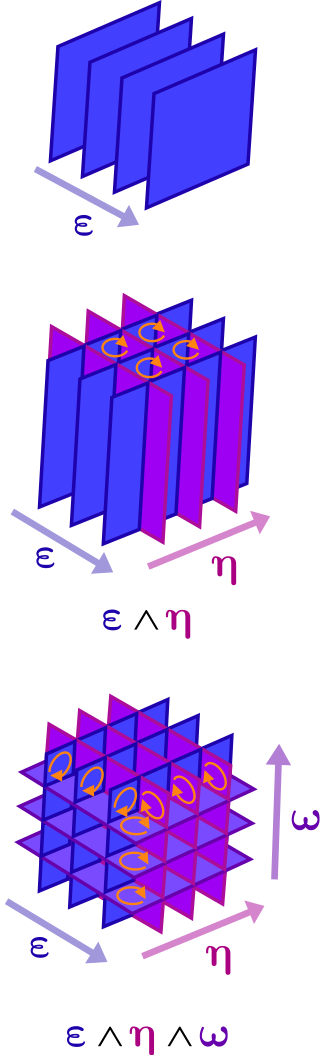
\includegraphics[scale=0.3]{figures/n-forme.png}
  \caption{Interprétation géométrique du produit extérieur de \(n\) co-vecteurs \(\varepsilon\), \(\eta\), \(\omega\) pour \(n = 1, 2, 3\). Les flèches circulaires correspondent à l'orientation (Wikipédia). }
  \label{n-forme}
\end{figure}

\begin{exemple}
  Si \(\alpha_i \in \Lambda ^{1}(E)\), (c.\`a.d. un co-vecteur \footnotemark, \(v_i \in E\),

  \begin{gather*}
    \alpha_1 \wedge \dots \wedge \alpha_m (v_1, \dots, v_m) = \sum_{\sigma \in S_m}^{} \operatorname{sgn}(\sigma) \alpha_1(v _{\sigma_1}) \dots \alpha_m(v _{\sigma_m}) = \operatorname{det}[\alpha_i(v_j)].
  \end{gather*}
\end{exemple}
\footnotetext{en \'equivalence: un \'el\'ement de $E^*$,  un tenseur covariant de type (0,1)}

\begin{exemple}
  \(\alpha_i : \mathbb{R}^3 \to \mathbb{R}\),

  \begin{gather*}
    \alpha_1(x^1, x^2, x^3) = x^1+x^2, \alpha(x^1, x^2, x^3) = x^3, \\
    v_1 = (1,1, 0), v_2 =(0, 1, 0).
  \end{gather*}

  \(m=2, n=3\).

  \begin{gather*}
    \alpha_1 \wedge \alpha_2(v_1, v_2) = \sum_{\sigma \in S_2}^{} \operatorname{sgn}(\sigma)\alpha_1(v _{\sigma_1}) \alpha_2(v _{\sigma_2}) \\
    = \alpha_1(v_1) \alpha_2(v_2) - \alpha_2(v_1) \alpha_1(v_2) = \operatorname{det}\left(\begin{pmatrix}
    \alpha_1(v_1) & \alpha_1(v_2) \\
    \alpha_2(v_1) & \alpha_2(v_2)
  \end{pmatrix}\right)  = \operatorname{det}\left(\begin{pmatrix}
    2 & 1 \\
    0 & 1
    \end{pmatrix}\right) = 2.
  \end{gather*}
\end{exemple}

\begin{prop}
  \(\alpha \in \Lambda ^{k}(E), \beta \in \Lambda ^{l}(E)\), alors \[\alpha\wedge \beta = (-1) ^{kl} \beta \wedge \alpha.\] En particulier, si \(k\) est impair,

  \[\forall \alpha \in \Lambda ^{k}(E), \alpha \wedge \alpha = 0, \]

  parce que dans ce cas, on a \(\alpha\wedge \alpha = (-1) \alpha\wedge \alpha\).
\end{prop}

\begin{proof}
  \begin{gather*}
    \alpha \wedge \beta(v_1, \dots, v _{k+l}) = \sum_{\sigma \in S _{k+l}}^{} \operatorname{sgn}(\sigma)(v _{\sigma_1}, \dots, v _{\sigma_k}) \beta(v _{\sigma _{k+1}}, \dots, v _{\sigma _{k+l}}) \\
    \beta \wedge \alpha(v_1, \dots, v _{k+l}) = \sum_{\sigma \in S _{k+l}}^{} \operatorname{sgn}(\sigma) \beta(v _{\sigma_1}, \cdots,  v _{\sigma_l}) \alpha(v _{\sigma_{l+1}}, \dots, v_{\sigma_{l+k}}).
  \end{gather*}

  On doit introduire \(\tau\) par
  \[
\forall i \in \{1, \cdots, l\}  \,\,\tau_i := i+k, \quad \forall i\in   \{l+1, \cdots, l+k\} \,\,\tau_{i} := i-l.
  \] et on observe que  telle que \( \operatorname{sgn} (\tau) = (-1) ^{kl}\) (exercice). Maintenant
  \begin{gather*}
    \beta \wedge \alpha(v_1, \dots, v _{k+l}) = \sum_{\sigma \in S _{k+l}}^{} \operatorname{sgn}(\sigma) \beta(v _{\sigma_1}, \cdots,  v _{\sigma_l}) \alpha(v _{\sigma_{l+1}}, \dots, v_{\sigma_{l+k}}) \\
 \stackrel{\sigma= \sigma' \tau}{=}   \operatorname{sgn}(\tau) \sum_{\sigma' \in S _{k+l}} \operatorname{sgn}(\sigma')  \beta(v _{\sigma'_{l+1}}, \dots, v_{\sigma'_{l+k}}) \alpha(v _{\sigma'_1}, \cdots,  v_{\sigma'_k})  \\
 = (-1)^{kl} \alpha\wedge \beta.
  \end{gather*}
\end{proof}

\begin{prop}
  Soit \(T \in \mathscr{L}(E, F)\). Pour tout \(k\), \( \Lambda ^{k}(T) : \Lambda ^{k}(F) \longrightarrow \Lambda ^{k}(E)\), pour \(\alpha \in \Lambda ^{k}(F), \beta \in \Lambda ^{l}(F)\),

  \[\underbrace{\Lambda ^{k+l}(T)(\alpha\wedge \beta)}_{ \in \Lambda ^{k+l}(E)} = \underbrace{\Lambda ^{k}(T)(\alpha)}_{\in \Lambda ^{k}(E)} \wedge \underbrace{\Lambda ^{l}(T)(\beta)}_{\in \Lambda ^{l}(E)}.\]
\end{prop}

La relation entre le produit extérieur \(\wedge\) et le produit extérieur des vecteurs de \(\mathbb{R}^3\) : soient \(v_1 = (x^1, x^2, x^3) \text{ et } v_2 = (y^1, y^2, y^3)\).

\[v_1 \times v_2 := (x^2 y^3 - x^3 y^2, x^3 y^1 - x^1 y^3, x^1 y^2 - x^2 y^1).\]

Penser à \(v_1, v_2\) comme des éléments de \((\mathbb{R}^3) ^{*}\), donc comme des éléments de \(\Lambda ^{1}((\mathbb{R}^3)^{*})\).

\begin{figure}[h!]
  \centering
  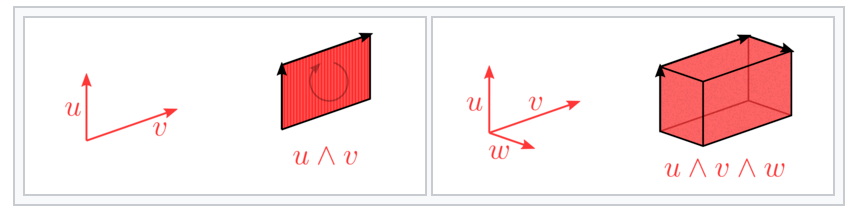
\includegraphics[scale=0.3]{figures/prod-ext-vect.png}
  \caption{Illustration du produit extérieur de vecteurs pour 2 et 3 vecteurs.}
  \label{}
\end{figure}

Quels sont les coefficients de \(v_1 \wedge v_2\) dans la base \(\epsilon _{12}, \epsilon _{13}, \epsilon _{23}\) ?

\begin{gather*}
  v_1 \wedge v_2 = \sum_{1 \leq  i_1 \less i_2 \leq 3}^{}  v_1 \wedge v_2 (e ^{i_1}, e ^{i_2})\epsilon_{i_1 i_2}  = v_1 \wedge v_2 (e ^{1}, e ^{2})\epsilon_{12} + v_1 \wedge v_2 (e ^{2}, e ^{3})\epsilon_{23} + v_1 \wedge v_2(e ^{1}, e ^{3})\epsilon_{13} \\
  = [v_1(e ^{1}) v_2(e ^{2}) - v_1(e ^{2}) v_2(e ^{1})]\epsilon_{12} + [v_1(e ^{2}) v_2(e ^{3}) - v_2(e ^{2}) v_1(e ^{3})]\epsilon_{23} + [v_1(e ^{1}) v_2(e ^{2}) - v_2(e ^{1}) v_1(e ^{3})]\epsilon_{13}\\
  = (e ^{1}(v_1) e ^{2}(v_2) - e ^{2}(v_1) e ^{1}(v_2))\epsilon_{12}+ (e ^{2}(v_1) e ^{3}(v_2) - e ^{2}(v_2) e ^{3}(v_1))\epsilon_{23} + (e ^{1}(v_1) e ^{2}(v_2) - e ^{1}(v_2) e ^{3}(v_1))\epsilon_{13} \\
  =(x^1 y^2 - x^2 y^1)\epsilon_{12} +(x^2 y^3 - x^3y^2)\epsilon_{23} + (x^1 y^3- x^3 y^1)\epsilon_{13}.
\end{gather*}

Donc si on choisit la base \(\{\epsilon_{23},\epsilon_{31},\epsilon_{12}\}\), on obtient \(\epsilon _{31} = -\epsilon_{13} = e _{1} \wedge e _{3}\). On obtient les coordonnées dans la base ordonnée \((\epsilon _{23},\epsilon_{31},\epsilon_{12})\) de \(\Lambda _{2}(\mathbb{R}^3)\) de \(v_1 \wedge v_2 \in \Lambda _{2}(\mathbb{R}^3)\) est donnée par \(v_1 \times v_2\).

\begin{figure}[h!]
  \centering
  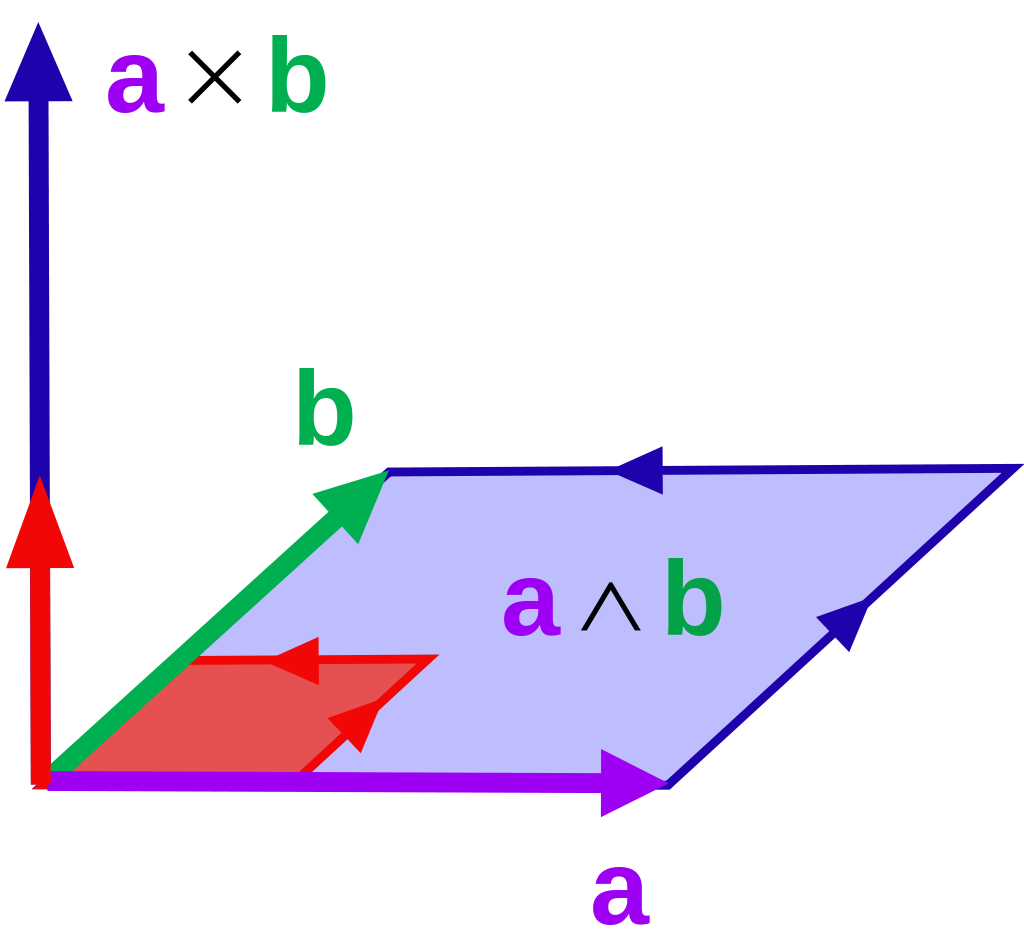
\includegraphics[scale=0.1]{figures/prod-cross-prod-ext.png}
  \caption{The cross product (blue vector) in relation to the exterior product (light blue parallelogram). The length of the cross product is to the length of the parallel unit vector (red) as the size of the exterior product is to the size of the reference parallelogram (light red) (Wikipédia).}
  \label{}
\end{figure}


\subsection{Contraction d'un tenseur par vecteur}

\begin{definition}[Contraction d'un tenseur par vecteur]
  Soit \(X \in E\). Pour tout \(\alpha \in \Omega ^{k}(E), 1 \leq k \leq n\). \(i_X (\alpha)\in \Omega ^{k-1}(E)\) pour

  \[i_X(\alpha)(v_1, \dots, v _{k-1}) \stackrel{\text{déf}}{=} \alpha(X,v_1, \dots, v _{k-1}).\]
\end{definition}

On a \(\Omega ^{0} \simeq \mathbb{R}\). Si \(\alpha \in \Omega ^{1}(E) = E ^{*}\), on a \(i_X(\alpha) = \alpha(X) \in \mathbb{R}\). En particulier, \(i_X\) est défini sur \(\Lambda ^{k}(E)\) pour tout \(k\).


\begin{lemma}
  \(X \in E, \alpha \in \Lambda ^{k}(E)\), alors \(i_X(\alpha) \in \Lambda ^{k-1}(E)\).
\end{lemma}

\begin{proof}

  Pour \(v_i = v_j, i \neq j, i, j \in \{ 1, \dots, k-1 \}\), donc
  \[i_X(\alpha)(v_1, \dots, v _{k-1}) = \alpha(X, v_1, \dots, v _{k-1}) = 0\]
\end{proof}

\begin{prop}

  \begin{enumerate}
    \item \(X \longrightarrow i_X\) est linéaire dans le sens que
    \begin{enumerate}
      \item \(i _{X+Y} = i_X+i_Y\),
      \item \(i _{cX} = c i _{X}\).
    \end{enumerate}

    \item Si on considère \(i_X\) restreint à \(\Lambda ^{*}(E)\), on a \(i_X \circ i_Y = - i_Y \circ i_X\) et \(i_X \circ i_X = 0\).
    \item Pour \(i _{X_{\mid \lambda ^{*}(E)}}\), on a, pour \(\alpha \in \Lambda ^{k}(E), \beta \in \Lambda ^{l}(E)\),

    \[i_X(\alpha \wedge \beta) = i_X(\alpha)\wedge \beta+ (-1) ^{k} \alpha \wedge (i_X \beta).\]
  \end{enumerate}

\end{prop}

\begin{remark}
 Supposons que \(F \subseteq E\) est un sous-espace vectoriel, avec \(\operatorname{dim}(F) = n-1, \operatorname{dim}(E) = n\), \(X \notin F\) et \(\omega\) est un élément de volume en E, alors \(\omega \in \Lambda ^{n}(E)\). Alors \(i_X(\omega) \in \Lambda ^{n-1}(F)\) va être un élément de volume pour \(F\). En effet  \(i_X(\omega) \in \Lambda^{n-1}(E) \). Donc quand on dit que \(i_X(\omega) \in \Lambda^{n-1}(F)\), on est en train de considérer  \(\Lambda ^{n-1}(I_F) (i_X(\omega))  = i_X(\omega)_{\mid  F^{n-1}}\)  en réalité:

  \[I_F : F \longrightarrow E \text{ est une injection } \implies \Lambda ^{n-1}(E) \stackrel{\Lambda ^{n-1}(I_F)}{\longrightarrow} \Lambda ^{n-1}(F), \]

  \[\Lambda ^{n-1}(I_F) (\alpha) (v_1, \dots, v _{n-1}) = \alpha(v_1, \dots, v _{n-1}), v_i \in F.\]

  Donc  $\Lambda ^{n-1}(I_F)(\alpha)$ est simplement la restriction de $\alpha : E^{n-1} \to \R$  sur le sous-espace $F^{n-1}$.


\end{remark}

\section{Analyse tensorielle sur les ouverts de \(\mathbb{R}^n\)}\marginnote{18-10-2023}

\subsection{Motivation}

On veut faire  de l'analyse (calcul différentiel) sur les surfaces, courbes, variétés (les objets courbes de dimensions supérieures).


\begin{figure}[h!]
  \centering
  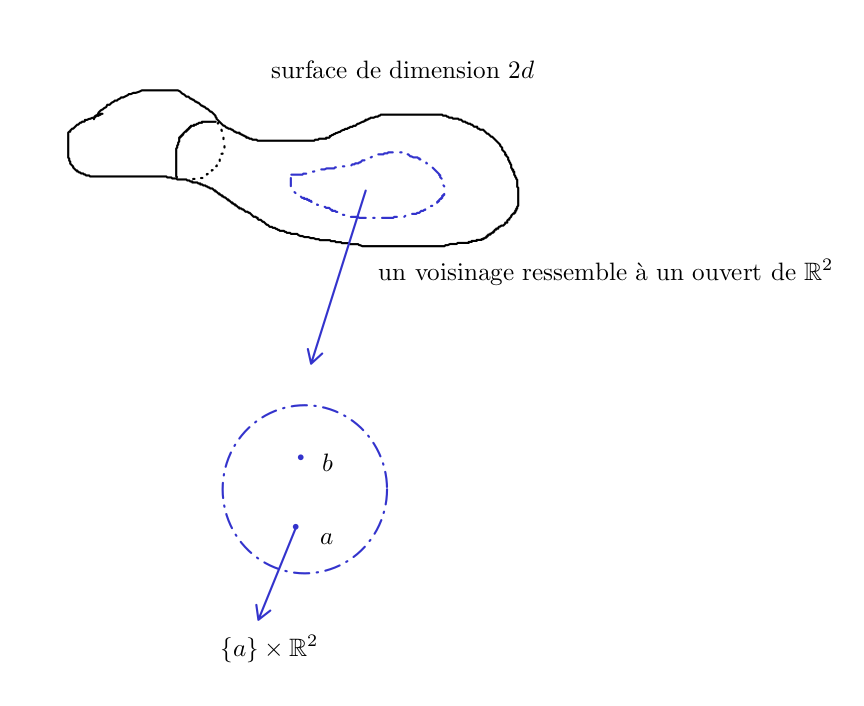
\includegraphics[scale=0.3]{figures/motiv1-corr.png}
  \caption{Dans ce cas, \(\mathbb{R}^2\) est tangent partout, mais on l'indexe par le point de base. }
  \label{}
\end{figure}

\begin{figure}[h!]
  \centering
  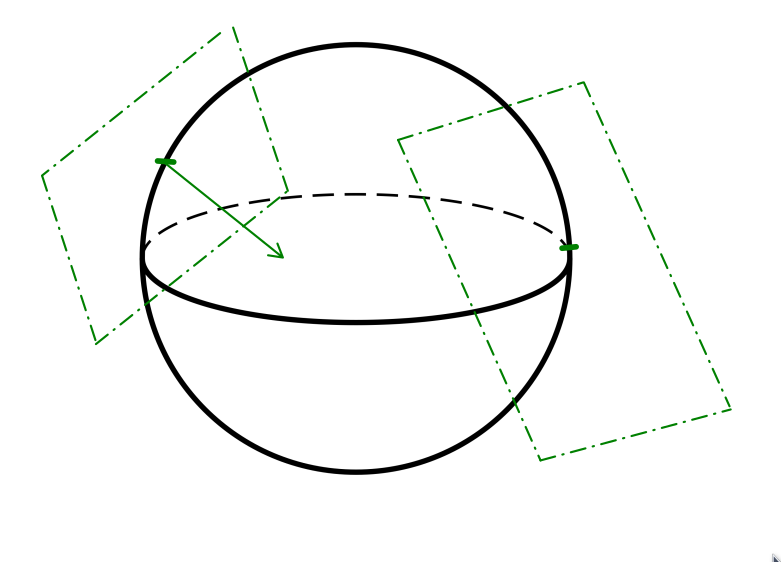
\includegraphics[scale=0.2]{figures/motiv2.png}
  \caption{En général, chaque vecteur tangent est à l'intérieur du plan tangent et chaque plan tangent est différent.}
  \label{}
\end{figure}


\subsection{L'espace tangent}
\begin{definition}
  Soit \(U \subseteq \mathbb{R}^2\) un ouvert. Pour tout \(a \in U\), l'espace tangent

  \[T_a U \stackrel{\text{déf}}{=} \{ a \} \times \mathbb{R}^{n},\]

  et est muni d'un espace vectoriel de manière suivante :

  \[\forall u,v \in \mathbb{R}^n, \underbrace{(a,u)}_{\in T_a U} + (a,v) = (a, u+v),\]

  \[\forall r \in \mathbb{R}, \forall v \in \mathbb{R}^n, r(a,u) = (a, ru).\]
\end{definition}

\(T_a U\) devient un espace vectoriel linéairement isomorphe à \(\mathbb{R}^n\). Géométriquement on peut penser à \(T_a U\) comme un vecteur de \(\mathbb{R}^n\) basé en un point \(a\).

\begin{figure}[h!]
  \centering
  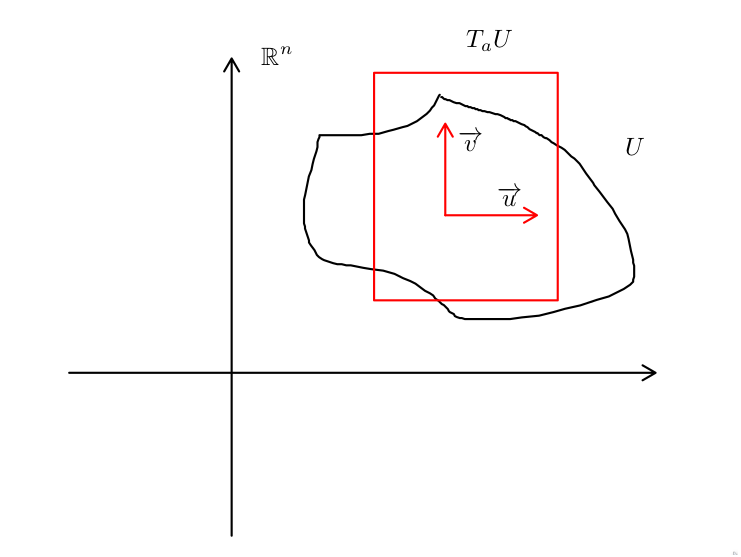
\includegraphics[scale=0.3]{figures/plan_tangent.png}
  \caption{Exemple d'un plan tangent à \(U\).}
  \label{}
\end{figure}

\subsection{Dérivation d'une fonction}

\begin{definition}
  Soit \(f : U \to \mathbb{R}^n\). Pour tout \(a \in U, Df(a) : \mathbb{R}^n \longrightarrow \mathbb{R}^m\). C'est une application linéaire.

  On va définir

  \[d_a f = df(a) : T_a U \longrightarrow \mathbb{R}^m,\]

  avec \[\underbrace{d f((a,\vec{v} ))}_{a \in U,\vec{v} \in \mathbb{R}^n  } = Df(a)(\vec{v}).\]

  Si \(a \neq b\), \(d_a f\) ne peut pas agir sur \(T_a U\) (formellement, ce n'est pas défini.

  On dit que \(d_a f\) est la dérivée (ou la différentielle) de \(f\) au point \(a\).
\end{definition}



\begin{remark}
  Si \(m=1\), \(d_a f \in \mathscr{L}(T_a U, \mathbb{R})\), c'est-à-dire que \(d_a f \in (T_a U) ^{*}\).
\end{remark}


\begin{remark}[Notation]
  \(T_a ^{*} U \stackrel{\text{déf}}{=} (T_a U)^{*} \simeq \{ a \} \times (\mathbb{R}^n)^{*}\).
\end{remark}



\subsection{Fibr\'es tensoriels}

\begin{definition}
  Le fibré tangent sur \(U\) est

  \[T U \stackrel{\text{déf}}{=} \bigcup _{a \in U} \underset{(a,\vec{ v } ), \vec{ v } \in \mathbb{R}^n }{T_a U} \simeq U \times \mathbb{R}^n\]

  et le fibré cotangent est \[T ^{*} U \stackrel{\text{déf}}{=} \bigcup _{a \in U} \underset{(a,f), f \in (\mathbb{R}^*)^{n}}{T_a ^{*} U} \simeq U \times (\mathbb{R}^{*})^{n}. \]
\end{definition}

Avec ce formalisme, la différentielle de \(f : U \longrightarrow \mathbb{R}^n\) est définie par \( df : U \longrightarrow T ^{*} U\) et \(\forall a \in U, d f(a) = d_a f \in T_a ^{*} U \subseteq T ^{*} U\).

\begin{remark}
  {\fontencoding{U}\fontfamily{futs}\selectfont\char 66\relax} Une condition nécessaire pour qu'une application \(\alpha : U \longrightarrow T ^{*} U\) soit une différentielle soit dans la forme \(\alpha = df\) est que pour tout \(a \in U, \alpha(a) \in T_a ^{*} U\).
\end{remark}

Si on définit \(\pi : T_a ^{*} U \longrightarrow U\) par \(\pi(a,f) = a\), cette condition nécessaire est équivalente que de dire que \(\pi \circ \alpha = \operatorname{id}_{U}\).

\begin{exemple}[De différentielle]
  Projection sur le composant \(j\) :

  On a \(x ^{ j} : U \longrightarrow \mathbb{R}\) telle que

  \[x ^{j}(a_1, \dots, a_n) = a_j.\]

  \[d_a x ^{j}(a, \vec{v}) = D x ^{j}(a)(\vec{v}) = \left[\frac{\partial x ^{j} }{\partial x^1}, \dots, \frac{\partial x ^{j} }{\partial x^n}\right] \left[\begin{matrix}
    v_1 \\
    \vdots \\
    v_n
  \end{matrix}\right] = [0, \dots, 0, \underset{\text{en } j}{1},0, \dots, 0] \left[\begin{matrix}
    v_1 \\
    \vdots \\
    v_n
  \end{matrix}\right] = v_j.\]
\end{exemple}

On a \(d x ^{j} : U \longrightarrow T ^{*} U\). Pour tout \(a \in U\), \(d x ^{j}(a) \in T_a^{*}U\).

Donc \(d x ^{j}(a) = (a,f)\) où \(f \in (\mathbb{R}^n)^{*}\). Pour tout \(\vec{ v }  \in \mathbb{R}^n\), \(f(\vec{v}) = v_j\). Pour \(e_i \in \mathbb{R}^n, f(e_i) = \delta _{i}^{j}\), donc \(f = e^j\), l'élément de la base duale. On a alors

\[d x ^{j}(a)=(a, e ^{j}).\]

Donc \((d x ^{1}(a), \dots, d x ^{n}(a))\) est une base naturelle pour \(T_a^{*} U\). La base duale de cette base dans \(T_a U \simeq (T_a ^{*}U)^{*}\) est décrite par la notation suivante :

\[\left(\frac{\partial  }{\partial x ^{1}}(a), \dots, \frac{\partial  }{\partial x ^{n}}(a)\right) = ((a,e_1), \dots, (a,e_n)).\]

On a \(\displaystyle\frac{\partial  }{\partial x ^{j}}(a) = (a, e_j), (d x ^{j}(a))\displaystyle\left(\frac{\partial  }{\partial x ^{i}}(a)\right) = \delta^{j}_{i}\).

\begin{figure}[h!]
  \centering
  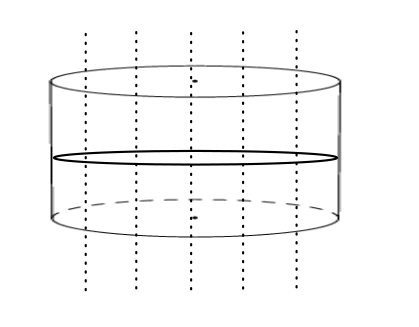
\includegraphics[scale=0.3]{figures/cylindre_tens.png}
  \caption{Cylindre \(S ^{1} \times [-1,1]\). On peut  le considérer comme une fibration sur $S ^{1}$. Le cylindre infini  \(S ^{1} \times \R\) va \^etre diff\'eomorphe avec le fibr\'e tangent $TS^1$ de $S^1$}
  \label{}
\end{figure}

\begin{figure}[h!]
  \centering
  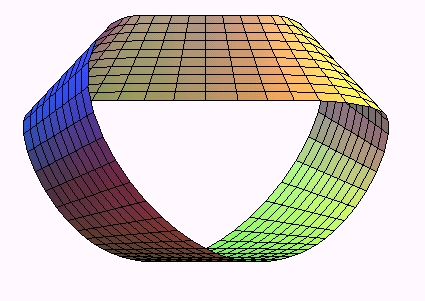
\includegraphics[scale=0.3]{figures/ruban_mobius.jpg}
  \caption{Le Ruban de Mobius est une fibration sur $S^1$ mais n'est pas équivalent à \(S ^{1} \times [-1, 1]\) (il n'est pas un sous ensemble du fibr\'e tangent $TS^1$). Similairement, il y a  par exemple des surfaces de dimension 2 $\Sigma$  dont le fibr\'e tangent $T\Sigma$ n'est pas \'equivalent \`a $\Sigma \times \R^2$.}
  \label{}
\end{figure}


On suppose que \(E= T_a U\). On peut construire \(\Omega ^{k}(T_a U), \Omega _{l}(T_a U) = \Omega _{l}(T_a ^{*} U), \Omega _{l}^{k}(T_a U)\) qui sont des \((l,k)\)-tenseurs sur \(T_a U\).

On peut aussi définir \(\Lambda ^{k}(T_a U)\) (tenseurs extérieurs covariants), \(\Lambda _{l}(T_a U) = \Lambda ^{l}(T_a ^{*}U)\) (tenseurs extérieurs contravariants), \(\Lambda ^{k}_{l}(T_a U)\).

\begin{definition}
  On définit \[(T ^{k}_{l})_a U = \Omega ^{k}_{l}(T_a U)\] et \[(\Lambda _{l}^{k})_a U  \stackrel{\text{déf}}{=} (\Lambda ^{k}_{l})(T_a U).\]
\end{definition}

Si \(k=l=0\), on ne va pas les écrire.

\begin{definition}
  On peut alors définir les fibrés tensoriels et tensoriels extérieurs par :

  \[T ^{k}_{l} U \stackrel{\text{déf}}{=} \bigcup _{a \in U} (T ^{k}_{l})_a U \text{  et } \Lambda ^{k}_{l} U \stackrel{\text{déf}}{=} \bigcup _{a \in U} (\Lambda ^{k}_{l})_a U.\]
\end{definition}



Très souvent on va avoir affaire aux fibrés où soit \(k\) soit \(l\) vaut 0. Par exemple,

\begin{gather*}
  \Lambda ^{k} U = \bigcup _{a \in U} \Lambda_a^{k} U = \bigcup _{a \in U} \Lambda ^{k}(T_a U), \\
  T ^{k} U = \bigcup _{a \in U} T_a ^{k} U = \bigcup _{a \in U} \Omega ^{k}(T_a U).
\end{gather*}

Si \(\alpha \in T _{l}^{k} U\), alors il existe \(a \in U\) tel que \(\alpha \in (T_l ^{k})_a U = \Omega ^{k}_{l}(T_a U)\). Donc \(\alpha\) est une application \((k+l)\)-linéaire sur \(\underbrace{T_a U \times \dots \times T_a U}_{k \text{ fois}} \times \underbrace{(T_a U)^{*} \times \dots \times (T_a U)^{*}}_{l \text{ fois}}\).

Mais une telle application peut être identifiée par une application \((k+l)\)-linéaire $\tilde{\alpha}$ sur \[\underbrace{\mathbb{R}^n \times \dots \mathbb{R}^n}_{k \text{ fois}} \times \underbrace{(\mathbb{R}^n)^{*} \times \dots \times (\mathbb{R}^n)^{*}}_{l \text{ fois}}\] avec les isomorphismes \(T_a U \simeq \mathbb{R}^n\), \(T_a ^{*} U \simeq (\mathbb{R}^n)^{*}\).

Donc \(\Omega ^{k}_{l}(T_a U) \simeq \{ a \} \times \Omega ^{k}_{l}(\mathbb{R}^n)\) avec l'identification $\alpha = (a, \tilde \alpha)$ et on a une projection bien définie sur la première composante

\[\tau _{l}^{k} : \Omega _{l}^{k}(T_a U) \longrightarrow U, \tau _{l}^{k}(a, \tilde{\alpha}) = a.\]

Donc si \(\alpha \in T _{l}^{k}U \), on a \(\tau _{l}^{k}(\alpha)\) est le point \(a \in U\) pour lequel \(\alpha \in (T _{l}^{k})_a U\).


\subsection{Champs tensoriels}

\begin{definition}
  Un champ de tenseurs ({\it champ tensoriel}) sur \( U \subseteq \mathbb{R}^n\) est une application

  \[\alpha : U \longrightarrow T _{l}^{k} U\]

  telle que \[\tau _{l}^{k} \circ \alpha = \operatorname{id}_{U}, \quad \text{c.\`a.d.} \,\,\forall a\in U \,\, \tau _{l}^{k}(\alpha(a))=a.\]
\end{definition}

\begin{figure}[h!]
  \centering
  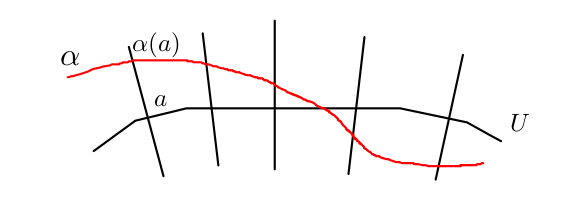
\includegraphics[scale=0.3]{figures/ch_tensoriel.png}
  \caption{Exemple d'un champ tensoriel comme section d'un fibré tensoriel.}
  \label{}
\end{figure}

\(\alpha\) est aussi appelée parfois une section du fibré tensoriel \(T ^{k}_{l} U\).

Si \(\alpha\) est un champ tensoriel, pour tout \(a \in U\), \(\alpha(a) \in \Omega _{l}^{k}(T_a U)\).

L'ensemble \((e ^{i_1} \otimes \dots \otimes e ^{i_k} \otimes e _{j_1} \otimes \dots \otimes e _{j_l})\) est une base de \(\Omega _{l}^{k}(\mathbb{R}^n)\) où \(1 \leq i_1, \dots, i_k, j_1, \dots, j_l \leq  n\). Maintenant la base de \(\Omega^{k}_{l}(T_a U)\) devient

\[d x ^{i_1}(a) \otimes \dots \otimes d x ^{i_k}(a) \otimes \frac{\partial }{\partial d x ^{j_1} }(a) \otimes \dots \otimes \frac{\partial  }{\partial x ^{j_l}}(a).\]

Donc pour tout \(a \in U\), il existe des coefficients \(a _{i_1 \dots i_k}^{j_1 \dots j_l}(a) \in \mathbb{R}\) tels que :

\[\alpha(a) = \sum_{\substack{1 \leq  i_1, \dots, i_k \leq  n \\ 1 \leq j_1, \dots, j_l \leq  n}}^{} a ^{j_1 \dots j_l}_{i_1 \dots i_k}(a) d x ^{i_1}(a) \otimes \dots \otimes d x ^{i_k}(a) \otimes \frac{\partial  }{\partial x ^{j_1}}(a) \otimes \dots \otimes \frac{\partial  }{\partial x ^{j_l}}(a).\]



Donc

\[\alpha = \sum_{1 \leq  i_1, \dots, i_k, j_1, \dots, j_l \leq  n} a _{i_1 \dots i_k}^{j_1 \dots j_l} d x ^{i_1} \otimes \dots \otimes d x ^{i_k} \otimes \frac{\partial  }{\partial x ^{j_1}} \otimes \dots \otimes \frac{\partial  }{\partial x ^{j_l}}\]

où \(a _{i_1 \dots i_k} ^{j_1 \dots j_l} : U \longrightarrow \mathbb{R}\) est une application (elle associe à chaque \(a \in U\) un coefficient réel).

\begin{definition}
  On dit que le champ vectoriel \(\alpha\) est de classe \(\mathcal{C}^r\) si \(\forall i_1, \dots, i_k, j_1, \dots, j_l\), le coefficient \[a _{i_1 \dots i_k}^{j_1 \dots j_l} \in \mathcal{C}^r(U).\]
\end{definition}

Donc on peut parler de régularité de \(\alpha : U \longrightarrow \mathbb{R} ^{n+ n ^{k+l}}\) directement, mais dans ce cas là, la définition revient à la même.

\subsection{Exemple très important : la métrique riemanienne}

\begin{definition}
  Soit \(U \subseteq \mathbb{R}^n\) ouvert. Une métrique riemanienne sur \(U\) est un champ tensoriel 2-covariant (de type (0,2), autrement dit \(\alpha : U \longrightarrow T_0 ^2 U\)) symétrique, positif-défini sur \(U\).
\end{definition}

Si \(g\) est une métrique riemanienne sur \(U\), \(g : U \longrightarrow T ^2 U\).

Pour tout \(x \in U, g(a) \in \Omega ^{2}(T_a U)\), (c.\`a.d. \(\tau ^2 \circ g = \operatorname{id}_{U}\)).

\[\forall \vec{ u }, \vec{ v } \in T_a U, \quad  g(a)(\vec{ u }, \vec{ v }  ) = g(a)(\vec{ v }, \vec{ u }) \text{ (symétrie)}.\]

\[\forall \vec{ u }  \in T_a U,\quad  g(a)(\vec{ u }, \vec{ u }) \ge 0;  \quad    g(a)(\vec{ u }, \vec{ u } )  =0 \Leftrightarrow u=0 \quad \quad \text{ (pos. d\'ef.)}.\]

Donc cela revient à dire que \(g(a)\) est un produit scalaire sur \(T_a U\) (mais qui dépend de \(a\)).

La métrique riemanienne est donc un champ tensoriel de type (0,2) tel que \(\forall a \in U\), \(g(a)\) est un produit scalaire sur \(T_a U\).

Donc \[g = \sum_{1 \leq  i_1, i_2 \leq n} g _{i_1 i_2} d x ^{i_1} \otimes d x ^{i_2} = \sum_{1 \leq i, j \leq n} g _{ij} d x ^{i} \otimes d x ^{j}.\]

\emph{Quelle est la condition sur les coefficients \(g _{ij}\) pour que \(g\) devienne une métrique riemanienne ?}

Pour tout \(x \in U\), on peut former la matrice \[G_a = [g _{ij}(a)]_{n \times n}.\]

\begin{prop}
  \(g(a)\) est une métrique riemanienne sur \(T_a U\) si et seulement si \(g(a)\) est un produit scalaire.
\end{prop}

\begin{lemma}
  \(g(a)\) est un produit scalaire sur \(T_a U\) si et seulement si \(G_a\) est une matrice symétrique définie positive.
\end{lemma}

\begin{proof}
  \begin{gather*}
    g(a)\left(\frac{\partial  }{\partial x ^{i'}}, \frac{\partial  }{\partial x ^{j'}}\right) = \sum_{1 \leq i, j \leq  n} g _{ij}(a) d x ^{i}(a) \otimes d x ^{j}(a) \left(\frac{\partial  }{\partial x ^{i'}}(a), \frac{\partial  }{\partial x ^{j'}}(a)  \right) \\
    = \sum_{1 \leq i,j \leq n} g _{ij}(a) d x ^{i}(a)\left(\frac{\partial  }{\partial x ^{i'}}(a) \right) d x ^{j}(a) \left(\frac{\partial  }{\partial x ^{j'}}(a) \right)  = \sum_{1 \leq i, j \leq n} g _{ij}(a) \delta _{i'}^{i} \delta _{j'}^{j} = g _{i'j'}(a).
  \end{gather*}

  Donc \(\forall i, j\),

  \[g _{i'j'}(a) = g(a) \left(\frac{\partial  }{\partial x ^{i'}}(a),\frac{\partial  }{\partial x ^{j'}}(a) \right) = g(a)\left(\frac{\partial  }{\partial x ^{j'}}(a),\frac{\partial  }{\partial x ^{i'}}(a) \right) = g _{j'i'}(a), \]

  ce qui implique que \(\prescript{t}{}G_a = G_a\), donc \(G_a\) est symétrique.
\end{proof}

Supposons que \(g(a)\) est défini positif.

\begin{gather*}
\forall v\in T_aU \quad   g(a)(\vec{v}, \vec{v}) = \sum_{i,j}^{} d x ^{i}(a) \otimes d x ^{j}(a)(\vec{v}, \vec{v}),
\end{gather*}

avec   $$\vec{v} = \sum_{j=1}^{n} v ^{j} \frac{\partial  }{\partial x ^{j}} (a).$$
Donc

\begin{gather*}
g(a)(\vec{v}, \vec{v})   =  \sum_{i,j}^{} g _{i,j}(a) d x^{i}(a) \otimes d x^{j}(a) \left(\sum_{i'}v ^{i'} \frac{\partial  }{\partial x ^{i'}}(a), \sum_{j'}^{} v ^{j'} \frac{\partial  }{\partial x ^{j'}}(a)\right) \\
 \sum_{i,j} \sum_{i',j'} g _{ij}(a) v ^{i'} v ^{j'} d x^{i}(a) \left(\frac{\partial  }{\partial x ^{i'}}(a) \right)   d x^{j}(a)  \left( \frac{\partial  }{\partial x ^{j'}}(a) \right)=\sum_{i,j} \sum_{i',j'} g _{ij}(a) v ^{i'} v ^{j'} \delta^{i}_{i'} \delta^{j}_{j'} \\
 \\ = \sum_{i',j} g _{i'j'}(a) v ^{i'} v ^{j'}
  = [v ^{1} \ \dots \ v ^{n}] [G_a] \left[\begin{matrix}
    v ^{1} \\
    \vdots \\
    v ^{n}
  \end{matrix}\right] = \tilde{\vec{v}} \cdot G_a \tilde{\vec{v}}.
\end{gather*}

%\begin{gather*}
%  \vec{v} = \sum_{j=1}^{n} v ^{j} \frac{\partial  }{\partial x ^{j}} = \sum_{i,j} g _{i,j} (a) d x ^{i}(a) \otimes d x ^{j}(a) \left(\sum_{i'} \frac{\partial  }{\partial x ^{i'}}(a), \sum_{j'} v ^{j'} \frac{\partial  }{\partial x ^{j'}}(a)\right) \\
%  = \sum_{i,j} \sum_{i',j'} g _{ij}(a)v ^{i'} v ^{j'} d x ^{i}(a) \left(\frac{\partial  }{\partial x ^{i'}}(a)\right)  d x ^{j}(a) \frac{\partial  }{\partial x ^{j'}}(a) \right)  = \sum_{\substack{i,j\\i' = i\\j'=j}} g _{ij}(a) v ^{i} v ^{j} \\
%  = [ v ^{1} \dots v ^{n}] [G_a] \left[\begin{matrix}
%    v ^{1} \\
%    \vdots \\
%    v ^{n}
%  \end{matrix}\right] = \tilde{\vec{v}} \cdot G_a \tilde{\vec{v}}.
%\end{gather*}

Donc \(\tilde{\vec{v}} \cdot G_a \tilde{\vec{v}} \geq 0\) pour tout \(\vec{v} \in \mathbb{R}^n\) et \(\tilde{\vec{v}} \cdot G_a \tilde{\vec{v}} = 0 \iff \tilde{\vec{v}} = 0\), ce qui implique que \(G_a\) est défini positif.

Le sens réciproque est démontré par les mêmes calculs.

\paragraph{Commentaires}

\begin{enumerate}
  \item Si \(G \in \R ^{n\times n}\) est symétrique et défini positif, alors \(\forall \vec{u}, \vec{v} \in \mathbb{R}^n\),

  \begin{gather*}
    \langle \vec{u} \mid \vec{v} \rangle _{G} := \vec{u} \cdot G \vec{v} = \prescript{t}{}\! \vec{u} \, G \vec{v} = \langle \vec{u} \mid G \mid \vec{v} \rangle
  \end{gather*}

  est un produit scalaire.

  \item Si \(\langle \vec{u} \mid \vec{v} \rangle _{*} \) est un produit scalaire sur \(\mathbb{R}^n\), alors il existe une matrice \(G\) dans \(\mathbb{R} ^{n\times n}\) symétrique, définie positive telle que

  \[\langle \vec{u},\vec{v} \rangle _{*} = \langle \vec{u} \mid G \mid \vec{v} \rangle,  \]

  avec \(G = [g _{ij}] _{i,j}\) et \(g _{ij} = \langle e _{i} \mid e _{j} \rangle _{*} \).
\end{enumerate}

Donc pour la métrique riemanienne,

\[g = \sum_{i,j} g _{ij} d x^{i} \otimes d x^{j}, \]

avec \[g _{ij}(a) = g(a) \left(\frac{\partial  }{\partial x ^{i}}(a), \frac{\partial  }{\partial x ^{j}}(a)\right).\]

Pour tout \(i\), \(\frac{\partial  }{\partial x ^{i}}(a) = (a, e_i) \in T_a U\) et

\[\left(\frac{\partial  }{\partial x ^{1}}(a), \dots, \frac{\partial  }{\partial x ^{n}}(a)\right)\]

est une base de \(T_a U = \{ a \} \times \mathbb{R}^n, a \in U\).

\(g : U \longrightarrow T ^2 U, \tau ^2 \circ g (a) = a, \forall a \in U\) si et seulement si \(\forall a \in U, g(a) \in T^2_a U\).

La métrique \(g\) est de classe \(\mathcal{C}^r\) si et seulement si \(\forall i, j, g _{ij} : U \longrightarrow \mathbb{R}\) est de classe \(\mathcal{C}^r\) (par définition).

\begin{exemple}[La métrique euclidienne]
  \[g_{eu} = \sum_{i=1}^{n} d x^{i} \otimes d x^{i}\]

c.\`a.d. \[\forall a \in U, G_a = I _{n \times n} \in \mathbb{R} ^{n \times n}.\]
\end{exemple}


\begin{definition}
  Supposons que \((x, \vec{v}) \in T_x U\) pour \(x \in U\). Alors  la norme de \((x, \vec{u}) \in T_xU \)   par rapport \`a la m\'etrique riemannienne $g$ est d\'efini par

\[
\left \Vert (x,\vec{u}) \right\Vert_g  := g(x) ((x,\vec u), (x, \vec u))^\frac 12
\]
\end{definition}

\begin{remark}[Exercice]
Si $\vec u \in T_aU$, $\displaystyle \vec u = \sum_{i=1}^n u^i \frac {\partial} {\partial x^i} (a)$, on a
$$
\|\vec u\|^2_g =  \sum_{i,j=1}^n g_{ij}(a) u^i u^j.
$$
\end{remark}

\begin{definition}
  Supposons que \((x, \vec{v}), (x, \vec{v}) \in T_x U\) pour \(x \in U\). Alors l'angle entre ces deux vecteurs est défini par

  \[\sphericalangle (x,\vec{u}), (x, \vec{v}) = \cos ^{-1}\left(\frac{g(x)((x,\vec{u}), (x,\vec{v}))}{\left\Vert (x,\vec{u}) \right\Vert _{g} \left\Vert (x,\vec{v}) \right\Vert_g  }\right).\]
\end{definition}



\begin{remark}[Rappel]
  Pour tout produit scalaire \(\langle \ \mid \ \rangle _{*}\), l'inégalité de Cauchy-Schwarz est valide, c'est-à-dire :

  \[\forall \vec{u}, \vec{v} \in E, \left\lvert \langle \vec{u} \mid \vec{v} \rangle  \right\rvert \leq  \langle \vec{u} \mid \vec{u} \rangle _{*}^{\frac{1}{2}} \langle \vec{v} \mid \vec{v} \rangle _{*} ^{\frac{1}{2}}.  \]

  Donc pour tout \(\vec{u}, \vec{v} \in T_x U, \left\lvert g(a)(\vec{u}, \vec{v}) \right\rvert \leq  \left\Vert \vec{u} \right\Vert _{g} \left\Vert \vec{v} \right\Vert _{g}\).
\end{remark}

\begin{definition}
  \((U,g)\) où \(g\) est une métrique riemanienne et \(U \subseteq \mathbb{R}^n\) est un exemple d'une variété riemanienne.
\end{definition}

\subsubsection{Longeur des courbes}
\begin{exemple}
  Supposons \(\gamma : [a,b] \longrightarrow U\)  de r\'egularit\'e \(\mathcal{C}^1\), avec \([a,b] \subset \mathbb{R}\).

  On a, pour \(\gamma(t) = (x ^{1}(t), \dots, x ^{n}(t) )\), \((\gamma)'(t) = (x ^{1})'(t), \dots, (x ^{n})'(t)\),

  \begin{gather*}
    L(\gamma) \stackrel{\text{d\'ef}}{=} \int_{a}^{b} \left\Vert \gamma'(t) \right\Vert  dt = \int_{a}^{b}(\gamma'(t) \cdot I _{n \times n} \gamma'(t)) ^{\frac{1}{2}}dt = \int_{a}^{b}\langle \gamma'(t) \mid \gamma'(t) \rangle ^{\frac{1}{2}}dt.
  \end{gather*}
\end{exemple}





  On va définir, pour \(\gamma : ]a,b[ \longrightarrow U\),

  \[T \gamma : \underbrace{T{]a,b[}}_{(t,\vec{v}), \vec{v} \in \mathbb{R}}  \longrightarrow \underbrace{T U}_{(c,\vec{w}), c \in U, \vec{w} \in \mathbb{R}^n}.\]

  \(g(\gamma(t))\) est un produit scalaire sur \(T _{\gamma(t)} U\) et

  \[T \gamma(t,\vec{v}) = (\gamma(t), \vec{v}\gamma'(t)).\]

  Choisissons \(\{ 1 \}\) comme base de \(\mathbb{R}\). Alors

  \begin{enumerate}
    \item \[T \gamma _{\mid T _{t}]a,b[} : T _{t} ]a,b[ \longrightarrow T _{\gamma(t)} U.\]

    \item \(T \gamma (t,1) = (\gamma(t), \gamma'(t))\), avec \((t, 1)\) élément de base pour \(T _{t} ]a,b[ = \{t\} \times \R\) (l'espace tangent).
  \end{enumerate}

\begin{definition}
  On définit pour toute courbe continue  $\gamma:[a,b] \to U$, diff\'erentiable sur \(]a,b[\),

  \[L _{g}(\gamma) \stackrel{\text{d\'ef}}{=} \int_{a}^{b}g(\gamma(t))(T \gamma(t,1),T \gamma (t,1))^{\frac{1}{2}} dt. \]

Cette d\'efinition peut \^etre  facilement \'etendue au cas des courbes diff\'erentiables par morceaux.
\end{definition}
\begin{remark}
Comme l'int\'egrande est toujours positive (ou nulle), la valeur de \(L_g(\gamma)\) est toujours d\'efinie comme un \'el\'ement de \(\R_{+} \cup \{+\infty\}\).
\end{remark}
Si \(g = \sum_{}^{} g _{ij} d x^{i} \otimes d x^{j}\) et \(G_c = [g _{ij}(c)], \forall c \in U\), on obtient

\[L _{g}(\gamma) = \int_{a}^{b} \langle \gamma'(t) \mid G _{\gamma(t)} \mid \gamma'(t) \rangle ^{\frac{1}{2}}dt.\]


\begin{remark}
Avec la notation qu'on a eue sur la norme \( \left\Vert  \cdot \right\Vert _{g} \), on a, pour tout \(\gamma : [a,b] \longrightarrow \mathbb{R}\) différentiable,

\[L _{g}(\gamma) = \int_{a}^{b} \Vert  \underbrace{  T \gamma(t,1)}_{(\gamma(t), \gamma'(t))} \Vert _{g} dt.\]
\end{remark}



\begin{exo}
  Si \(x, y \in U, x \neq y\),  et \(\gamma : [a,b] \longrightarrow U\) est continu et de re\'gularit\'e \(\mathcal{C}^1\) sur \(]a,b[\), tel que \(\gamma(a)=x, \gamma(b)=y\)      alors \(L_g(\gamma) \bg 0\). \\

  {\it Indication:} Si \(\gamma'(t) = 0\), alors \( \gamma(t) \equiv \text{constant} \implies x=y \text{ impossible}\). Il existe \(t_0 \in ]a,b[\) tel que \(\gamma'(t_0) \neq 0 \implies \langle \gamma'(t_0) \mid G _{\gamma(t_0)} \mid \gamma'(t_0) \rangle  \bg 0\). Utiliser la continuité des acteurs pour conclure.
\end{exo}





\subsubsection{Rappel : distance, espace métrique}


 \begin{definition}
 Soit $U\subset \R^n$ un ouvert et $g$ une m\'etrique riemannienne sur $U$. On d\'efinit la distance riemannienne par rapport \`a la
 m\'etrique $g$  enter  $x,y\in U$ par
 \[
d _{g}(x,y) \stackrel{\text{d\'ef}}{=} \inf \{ L _{g}(\gamma), \gamma : [a,b] \longrightarrow U \ \text{continue, et différentiable sur } ]a,b[, \gamma(a) = x, \gamma(b)=b\}.
\]
\end{definition}

\begin{thm}
  Si \( U \subseteq \mathbb{R}^n\) connexe par arcs et \(g\) est une métrique riemanienne continue sur \(U\), alors

  \[d_g : U \times U \longrightarrow \mathbb{R}\]

  est une distance sur \(U\) et \((U, d_g)\) devient un espace métrique.
\end{thm}

\begin{remark}[Point technique]
  Si \(U\) est connexe par arcs, \(\forall x, y \in U, \exists \gamma \in \mathcal{C}^0([0, 1], U)\), avec \(\gamma(0) = x, \gamma(1) = y\), alors (analyse réelle, on utilise le fait que \(U\) est ouvert) il existe \(\gamma \in \mathcal{C}^1([0,1], U)\) avec \(\gamma(0)=x, \gamma(1)=y\).
\end{remark}

Donc il existe un élément de \(\{ \gamma \in \mathcal{C}^1([a,b], U) \mid \gamma(a) = x, \gamma(b) = y\}\), avec \(a = 0, b=1\). Comme \(\gamma \in \mathcal{C}^1([a,b])\), \(\left\lvert \gamma'(t)\right\rvert\) est continue sur \([a,b]\) implique que il existe \(M \bg 0 \) tel que \( \forall t \in [a,b], \left\Vert \gamma'(t) \right\Vert \leq M\) et \(G _{\gamma(t)} :  [a,b] \longrightarrow \mathbb{R}^{n \times n}\) est aussi continue.

Cela implique que \( t \longmapsto \langle \gamma'(t) \mid G _{\gamma(t)} \mid \gamma'(t)\rangle\) est continue sur \([a,b]\), ce qui implique que il existe \(\widetilde{M}\) tel que

\[\forall t \in [a,b], \langle \gamma'(t) \mid G _{\gamma(t)} \mid \gamma'(t) \rangle ^{\frac{1}{2}} \leq \widetilde{M},\]

ce qui implique que

\[L _{g}(\gamma) = \int_{a}^{b}\langle \gamma'(t)\mid G _{\gamma(t)} \mid \gamma'(t) \rangle \leq \widetilde{M}(b-a) \less + \infty, \]

donc \(d_g(x,y)\) ne peut être \(+\infty\), \(d_g(x,y) \in \mathbb{R} _{+}\). Donc \(d_g : U \times U \longrightarrow \mathbb{R}\) est justifié.

\begin{remark}

  \

 \begin{enumerate}
    \item Si \(U\) n'est pas connexe, il faut faire attention que le chemin droit de \(x\) à \(y\) peut sortir de \(U\) et n'est pas éligible pour évaluer \(L _{g}(\gamma)\).
    \item Même si \(U\) est connexe, il n'y a pas de raison que le chemin sur le segment droit joignant \(x\) à \(y\) soit le chemin le plus court :

    \[\gamma(t) = x + t(y-x), \gamma : [0, 1] \longrightarrow U.\]

    Il peut arriver que \[d_g(x,y) \less L_g(\gamma) = \int_{0}^{1} \langle y-x \mid G _{\gamma(t)} \mid y-x \rangle dt. \]

    \item Pas toutes les métriques \(d\) des espaces métriques \((X,d)\) où \(X\) est un ouvert de \(\mathbb{R}^n\) sont  les distances \(d_g\) pour une métrique riemanienne. Par exemple, {\bf (exercice)} la distance discr\`ete  \[d(x,y) = 1 \text{ si } x\neq y \text{ et sinon } d(x,y) =0\] ne peut pas \^etre dériv\'ee d'une métrique riemanienne.

    \item On peut remplacer les chemins \(\gamma\) par les chemins \(\mathcal{C}^1\) par morceaux ou bien par les chemins polygonaux.
  \end{enumerate}
\end{remark}


\begin{definition}
On dit que la courbe continue $\gamma :[a,b] \to U$ de r\'egularit\'e \(\mathcal{C}^1\)  sur $]a,b[$ est {\it r\'eguli\`ere} quand  $\forall t\in ]a,b[$,
$\gamma'(t) \neq 0$. On dit que $\gamma$ est {\it simple} quand elle est injective sur $]a,b[$.
\end{definition}

 \begin{exo}\label{par-arc} Soit \(U \subset \R^n\) un ouvert et $g$ une m\'etrique riemannienne sur \(U\). Soit $x,y
\in U$ et $\gamma : [a,b] \to U$ une courbe r\'eguli\`ere avec $\gamma(a) =x$, $\gamma(b)=y$.


\begin{enumerate}


\item[(a)] Soit $ t:[c,d] \to [a,b]$ une application continue de r\'egularit\'e \(\mathcal{C}^1\)\, sur \(]c,d[\) telle que
\[
t(c) =a, \,\, t(d) =b \quad \forall s\in ]c,d[ \quad t'(s) \neq 0
\]  On consid\`ere \(\eta : [c,d] \to U\)   d\'efini par \(\eta:= \gamma \circ t\). D\'emontrer que \(L_g(\eta) = L_g(\gamma)\).


\item[(b)] Soit $L:= L_g(\gamma)$. On d\'efinit pour $t\in [a,b]$
\[
s(t):= L_g(\gamma_{\mid [a,t]})
\]  D\'emontrer que \(s:[a,b] \to [0,L]\) est inversible avec l'application inverse \(t: [0,L] \to [a,b]\) continue de r\'egularit\'e \(\mathcal{C}^1\)\, sur \(]0,L[\) telle que
\[
t(0) =a, \,\, t(L) =b \quad \forall s\in ]0,L[ \quad t'(s) \neq 0.
\] On met $\eta :=  \gamma \circ t$.
 En d\'eduire que \( L_g(\eta) =   L_g (\gamma)\) et que
\[\forall s \in [0, L] \quad \|T\eta(s,1)\|_g = 1.
\] (\(\eta\) est le param\'etrage par la longueur d'arc de $\gamma$.)
\end{enumerate}
\end{exo}


  \subsubsection{M\'etriques conformales}

\begin{definition}
  Si pour une métrique riemanienne \(g\) donnée sur \(U\), il existe une fonction \(h : U \longrightarrow \mathbb{R}\) telle que

  \[\forall a \in U, g(a) = h(a)  \sum_{i}^n dx^i(a) \otimes dx^i (a) \quad \text{c.\`a.d. \,\,} G_a = h(a) I _{n \times n} = \left[\begin{matrix}
    h(a) & \dots & 0 \\
    \vdots & \ddots & \vdots \\
    0 & \dots & h(a)
  \end{matrix}\right].\]


  On dit que \(g\) est une métrique conformale.
\end{definition}


\begin{thm}
  Si \(g\) est une métrique conformale sur \(U\) et \(\vec{u}, \vec{v} \in T_a U\) pour \(a \in U\), alors

  \[\sphericalangle _{g} \vec{u}, \vec{v} = \sphericalangle \vec{u}, \vec{v}.\]

C.\`a.d. les angles entre les vecteurs sont les m\^emes pour $g$ et la métrique standard euclidienne.
\end{thm}

  \subsubsection{Le plan hyperbolique}

\begin{exemple}[Demi-plan de Poincaré (exemple de variété riemanienne) de dimension 2 et de géométrie non-euclidienne]

  \[U :=  \{ (x,y) \in \mathbb{R}^2 \mid y \bg 0 \}.\]

  On définit une métrique riemanienne sur \(U\) par

  \begin{gather*}
    g = \sum_{i=1}^{2}  g _{ii} d x^{i} \otimes d x^{i},  \\
    \text{c.\`a.d. pour}\,\,  x= x^1, y=x^2  \quad g _{ij}(x,y) =   \frac{1}{y ^2}\delta _{ij} \quad G _{(x,y)} = \left[\begin{matrix}
    \frac{1}{y ^2} & 0 \\
    0 & \frac{1}{y ^2}
  \end{matrix}\right].
  \end{gather*}
  \end{exemple}


Donc la métrique de Poincar\'e sur le demi-plan, qui peut-\^etre \'ecrite sous la forme

\[g(x,y) = \frac{1}{y ^2}(dx \otimes dx + d y \otimes d y)\]

est une métrique riemannienne conformale avec $\displaystyle h(x,y) = \frac {1}{y^2}$.

Si \(\vec{w} \in T _{(x,y)} U\) pour \((x,y) \in U\) quelconque, avec \(\vec{w} = (w_1, w_2)\), on a :

\[\left\Vert \vec{w} \right\Vert _{g} = (g(x,y)(\vec{w}, \vec{w})) ^{\frac{1}{2}} = \left(\frac{1}{y ^2} \left\Vert \vec{w}^2 \right\Vert \right) ^{\frac{1}{2}} = \frac{\left\Vert \vec{w} \right\Vert }{y}.\]


La géométrie induite par \(g\) sur le demi-plan est la géométrie hyperbolique, connue aussi sous le nom de la géométrie de Lobachevsky.


\begin{figure}[h!]
  \centering
  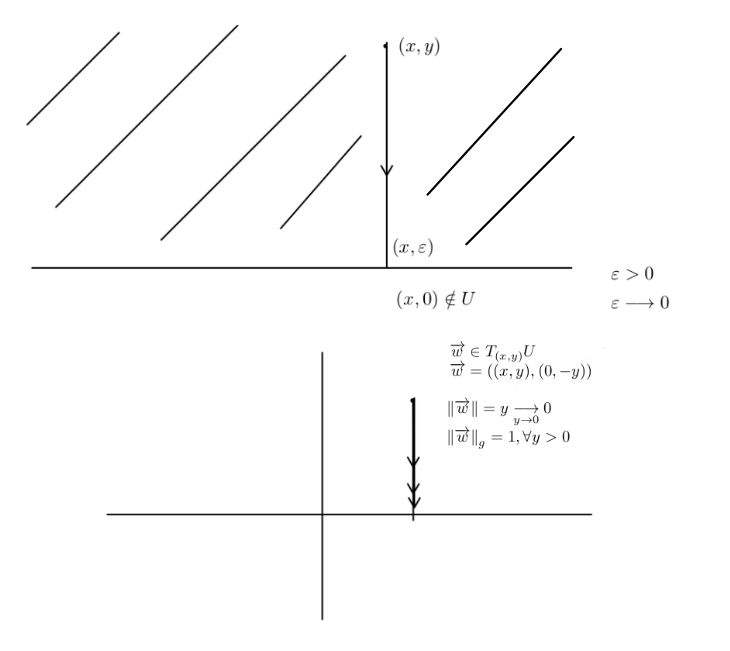
\includegraphics[scale=0.2]{figures/horizon1_corr2.png}
  \caption{}
  \label{horizon1}
\end{figure}

%\textcolor{red}{Correction  :} \textcolor{blue}{Exemple $\vec w \in T_{(x,y)} U$, $\vec w = ((x,y), (0,-y))$}

\begin{figure}[h!]
  \centering
  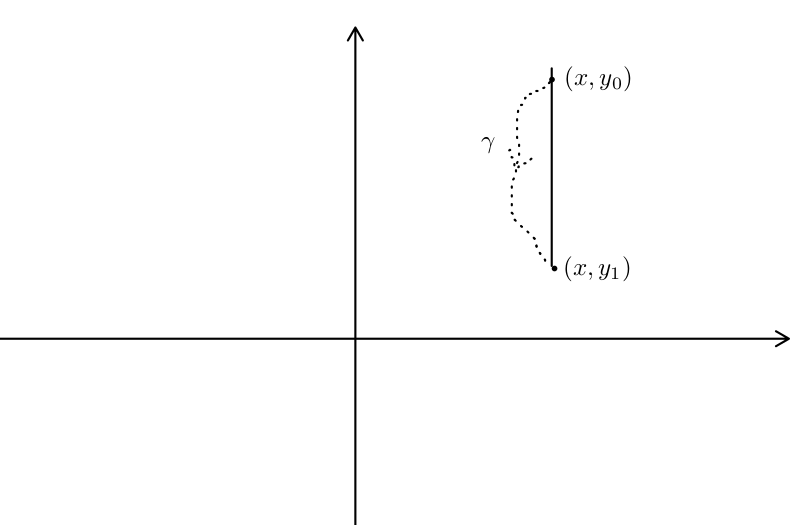
\includegraphics[scale=0.3]{figures/horizon2.png}
  \caption{}
  \label{horizon2}
\end{figure}


\subsubsection{G\'eod\'esies du demi-plan de Poincar\'e}

On a, pour le cas des figures \ref{horizon1} et \ref{horizon2}, le calcul suivant, pour \(\gamma(t) = (x(t), y(t))\) :

\begin{gather*}
  L_g(\gamma) = \int_{0}^{1}  \Vert \overbrace{(\gamma(t), \gamma'(t))}^{\in T _{{\gamma}(t)}U} \Vert_g  dt = \int_{0}^{1} \frac{\left\Vert \gamma'(t) \right\Vert }{y}dt = \int_{0}^{1} \frac{\sqrt{(x')^2(t)+ (y')^2(t)}}{y(t)} dt.
\end{gather*}

On a \(\eta(t) = (x,y_0) + t((x,y_1)-(x,y_0)) = (x,y_0 + t(y_1 - y_0))\) et \(\eta'(t) = (0,y_1-y_0)\), ce qui donne \(\left\Vert \eta'(t)\right\Vert   = \left\lvert y_1 - y_0 \right\rvert  \). Donc

\begin{gather*}
  L_g(\eta) = \int_{0}^{1} \frac{\left\Vert \eta'(t) \right\Vert }{y_0 + t(y_1-y_0)}dt = \int_{0}^{1} \frac{\left\lvert y_1-y_0 \right\rvert}{y_0 + t(y_1-y_0)}dt.
\end{gather*}

Notez que si l'on choisit \(\tilde{\gamma}(t)=(x,y(t))\) en partant de \(\gamma(t) = (x(t),y(t))\), on a :

\begin{gather*}
  L_g(\tilde{\gamma}) = \int_{0}^{1} \frac{\left\Vert \tilde{\gamma}(t) \right\Vert }{y(t)}dt = \int_{0}^{1} \frac{\left\lvert y'(t) \right\rvert}{y(t)}dt \leq  \int_{0}^{1} \frac{\sqrt{(x')^2(t) + (y')^2(t)}}{y(t)}dt = L_g(\gamma).
\end{gather*}

\begin{figure}[h!]
  \centering
  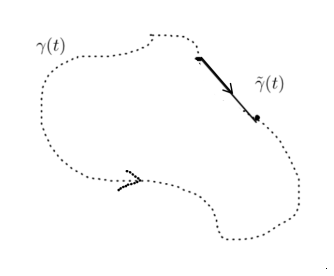
\includegraphics[scale=0.4, angle=-41]{figures/chemin-vert-court-corr2.png}
  \caption{Le chemin tout droit vertical est toujours le plus court (ici, \(\gamma\) est la courbe en pointillés, et \(\widetilde{\gamma}\) est la courbe noire). \textcolor{red}{l'image \`a corriger}}
  \label{chemin-vert-court}
\end{figure}

%\textcolor{red}{CORRECTION:  J'ai corrig\'e l'angle mais l'image est encore vague: $\gamma$ est quelle courbe ici?}

En conclusion, on a \(L_g(\tilde{\gamma}) \leq L_g(\gamma)\), ce qui signifie que le chemin le plus court par rapport à tous les chemins qui joignent \((x,y_0)\) à \((x,y_1)\) doit \^etre tout droit vertical comme illustré dans la figure \ref{chemin-vert-court}.

{\fontencoding{U}\fontfamily{futs}\selectfont\char 66\relax} On n'a pas encore dit que \(\eta\) donne le param\'etrage du chemin le plus court entre \((x,y_0)\) et \((x,y_1)\).   Voir Exercices \ref{par-arc} et \ref{vertical}.


\begin{figure}[h!]
  \centering
  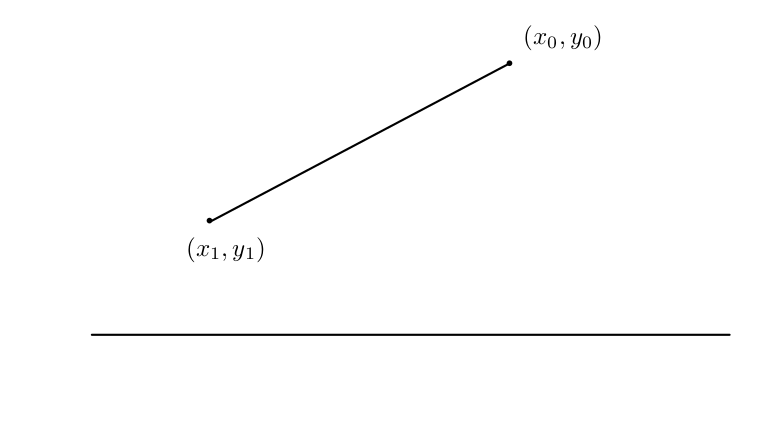
\includegraphics[scale=0.3]{figures/ligne-pas-tres-courte.png}
  \caption{La ligne droite n'est pas en général le chemin le plus court.}
  \label{}
\end{figure}

\


Si \(\gamma : [0, \infty) \longrightarrow U\),   \(\gamma(0) = (x_0, y_0)\), pour  \(\vec{w} =(0, -y) \in T _{(x,y)} U\), on a $\|\vec w\|_g =1$. On cherche donc \(\gamma(t)\) tel que

  \[ T\gamma (t,	1) = (\gamma(t), (0,-\gamma_2(t))  \in T_{\gamma(t)} U \quad  \text{c.\`a.d.} \quad \gamma'(t) =(0, -\gamma_2(t)),\]

avec \(\gamma(t) = (x(t), y(t)), \gamma_1(t) = x(t), \gamma_2(t) = y(t)\),

\[\begin{cases}
  x'(t) =0,   \\
  y'(t)=- y(t),
\end{cases}\]

alors \(y(t) = y_0 e^{-t} \). Donc \(\gamma(t) = (x_0, y_0 e^{-t})\) est le chemin partant de \((x_0, y_0)\) d'une manière verticale vers l'horizon \(y=0\) avec la vitesse hyperbolique constante.

On voit bien que \(\gamma(t) =(x_0, 0)\) donne \(t = +\infty\).

\begin{exo}\label{vertical}
Soit $x_0 \in \R$, $y_0  > y_1 > 0$,
\[ \eta:[0, 1]  : \to U, \,\, \eta(t):=  (x_0,y_0 + t(y_1 - y_0))\]
 et
 \[
\gamma :[0, \log(y_0/y_1)] \to U, \,\,  \gamma(t) = (x_0, y_0 e^{-t})
\]

\begin{enumerate}
\item[(a)] D\'emontrer que $\eta$ est une courbe r\'eguli\`ere, et que $\gamma$ est son param\'etrage par la longeur d'arc. En d\'eduire que
\[
L_g(\eta) = L_g(\gamma) = \log(y_0/y_1).
\]
\item[*(b)] D\'emontrer que \( d_g((x_0, y_0) , (x_0, y_1))  = \log(y_0/y_1). \)
\end{enumerate}
\end{exo}

Il faudra encore développer les techniques nécessaires pour pouvoir démontrer que les lignes droites par rapport à la métrique hyperbolique sur le demi-plan de Poincaré sont effectivement des demi-cercles centrés sur la ligne \(y=0\). Ces lignes droites sont appelées les géodésies de \((U,g)\) dans la géométrie différentielle.

Voici une première définition de la géodésie \ref{geodesie} (de manière rudimentaire plus géométrique que mécanique) :

\begin{definition}
  On dit que \(\gamma([a,b])\) est un segment géodésique dans \((U,g)\) si pour \(x = \gamma(a), y = \gamma(b), x, y \in U\),

  \[d _{g}(x,y) = L _{g}(\gamma).\]


\end{definition}



\begin{figure}[h!]
  \centering
  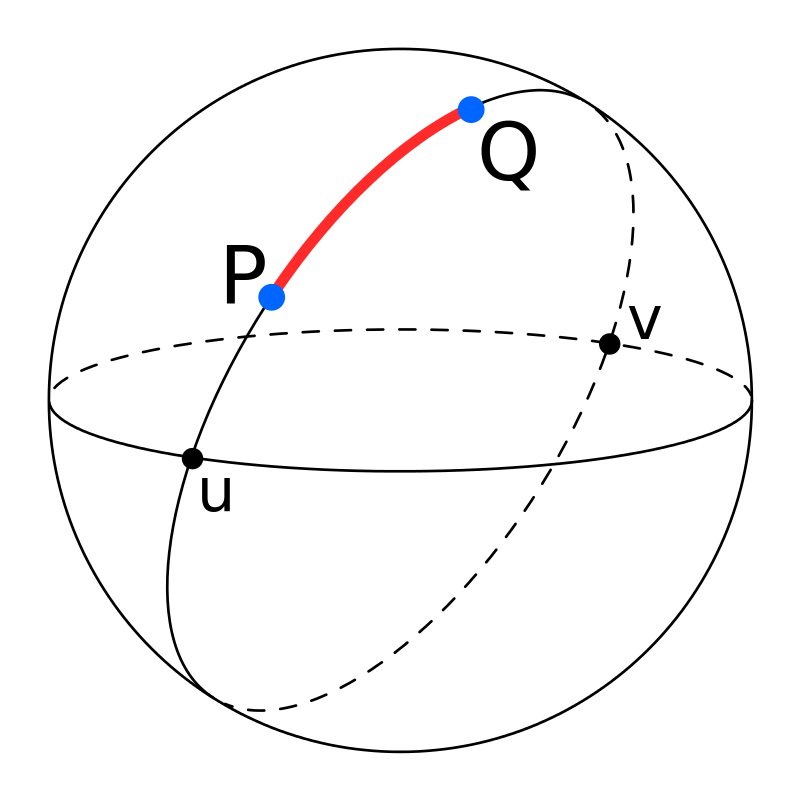
\includegraphics[scale=0.2]{figures/geodesie.png}
  \caption{Géodésie}
  \label{geodesie}
\end{figure}




\begin{definition}
  On dit que \(\mathscr{C}\) est une g\'eod\'esie de $(U,g)$ si pour tout point $z\in \mathscr{C}$, il existe un segment géodésique $\gamma([a,b])$ t.q. $\exists t\in ]a,b[$ t.q.  $\gamma(t) = z$ et $ \gamma([a,b]) \subset \mathscr{C}$. Ce concept est illustré dans la figure \ref{geodesie}.
 \end{definition}


\begin{remark}

 On va voir qu'une courbe de r\'eguarit\'e $\mathcal{C}^1$, \(\mathscr{C} \subseteq U\) est une géodésie de \((U,g)\) quand

  \[\mathscr{C} = \bigcup _{i \in I} \mathscr{C}_i \]

  où chaque \(\mathscr{C}_i\) est un segment géodésique tel que \(\forall n \in \mathbb{Z}, \mathscr{C}_n \cap \mathscr{C}_{n+1}\) est un singleton.
\end{remark}




\begin{remark}
On apprendra qu'il y a en parall\`ele une autre d\'efinition {\it m\'ecanique} plus fine de la notion de g\'eod\'esie. La fa\c con de param\'etriser la courbe  devient importante dans la formulation dite m\'ecanique.   N\'eanmoins, si la m\'etrique $g$ est assez  r\'egulier (p.ex. \( g\in \mathcal{C}^2\)), les images de courbes correspondantes \`a ces deux notions se co\"incident.
 \end{remark}


\subsubsection{Le disque de Poincaré}

 Le disque de Poincar\'e est un autre mod\`ele de la g\'eom\'etrie hyperbolique qui est donn\'ee par une m\'etrique riemannienne sur $U$ \'etant le disque d'unit\'e  dans $\R^2$ (cf figure \ref{escher}).  On va voir que le disque de Poincar\'e et le demi-plan de
Poincar\'e sont {\it isom\'etriques\footnote{Notion \`a d\'efinir.}}.



\begin{figure}[h!]
  \centering
  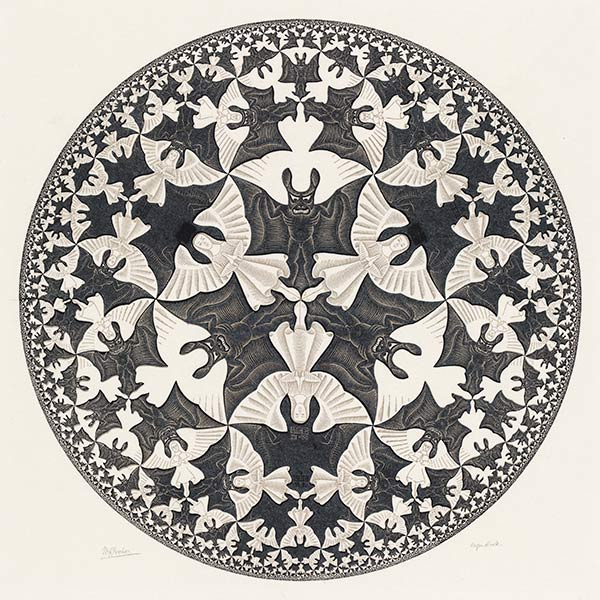
\includegraphics[scale=0.3]{figures/escher.jpg}
  \caption{Escher hyperbolic disc}
  \label{escher}
\end{figure}


 \subsubsection{Le gradient}

\begin{remark}[Rappel]
  Soit \(\beta : E \times E \longrightarrow \mathbb{R}\) un produit scalaire sur un espace vectoriel \(E\). Soit \(f \in E ^{*}\), avec \(\operatorname{dim}(E) = n\). Alors il existe un vecteur \(\overrightarrow{v_f}\) unique tel que

  \[\forall \overrightarrow{w} \in E, f(\overrightarrow{w}) = \beta(\overrightarrow{v_f}, \overrightarrow{w}).\]
\end{remark}

\begin{exemple}
  Soit \(\beta \in \Omega^2(\R^n)\) donné par la matrice \(B \in \mathbb{R}^{n \times n}\) symétrique définie positive sur une base \((e_1, \dots, e_n)\) de \(E = \R^n\), et $f\in E^*$. On cherche $\overrightarrow{v_f}$ t.q.
  \[
   \forall \vec w \in E \quad f(\vec w)= \beta(\overrightarrow{v_f}, \vec{w}) \,\, (= \langle \overrightarrow{v_f} \mid B \mid \vec{w} \rangle).
  \]
 On a

  \[f(\vec{w}) = f \left(\sum_{i} w^i e_i \right) = \sum_{i=1}^n w^i f(e_i), \]

  avec \(\overrightarrow{v_f} = \displaystyle \sum_{j=1}^{n} x^j e_j \) (\((x^1, \dots, x^n)\) inconnues), on obtient

  \begin{gather*}
    \beta(\vec{v_f}, \vec{w}) = \langle \vec{v_f} \mid B \mid \vec{w} \rangle = \sum_{i,j=1}^{n} x^i b _{ij} w^j,
  \end{gather*}

  \(B = [b _{ij}] _{n \times n}\). On veut que

  \[\forall (w^j)_{j=1}^{n} \quad \sum_{j=1}^n w^j f(e_j) = \sum_{i,j=1}^n x^i b _{ij} w^j\]

  qui est vrai si et seulement si

  \[\forall j\quad \sum_{i=1}^{n} x^i b _{ij}   = f(e_j) \in \mathbb{R}.\]

  \begin{equation}\label{truc-long}
   \left[\begin{matrix}
      x^1  &
      \cdots  &
      x^n
    \end{matrix}\right]   [b _{ij}]  = \prescript{t}{} [b_{ij}]\left[\begin{matrix}
      x^1 \\
      \vdots \\
      x^n
    \end{matrix}\right] = \left[\begin{matrix}
      f(e_1) \\
      \vdots \\
      f(e_n)
    \end{matrix}\right].
  \end{equation}

  \(f\) étant donné, comme \(\operatorname{det}(B) \neq 0\), il existe un unique \(x = (x^1, \dots, x^n) \in \mathbb{R}^n\) qui satisfait \ref{truc-long}, et donc

  \[\vec{v_f} = \sum_{i} x^i e_i \] est la réponse unique.
\end{exemple}

\begin{definition}[Rappel : gradient euclidien]
  Soit \(f : U \longrightarrow \mathbb{R} \text{ différentiable } , U \subseteq \mathbb{R}^n\). Le  gradient de $f$ est  donn\'e par

  \[\nabla f(a) = (\partial_1 f(a), \dots, \partial_n f(a)).\]
\end{definition}

\(Df(a) : \mathbb{R}^n \longrightarrow \mathbb{R}\) application linéaire de \((\mathbb{R}^n)^{*}\).

\[\forall \vec{v} \in \mathbb{R}^n\quad  Df(a)(\vec{v}) = \langle \nabla f(a), \vec{v}\rangle\]

avec la métrique euclidienne.

\

Soit \((U,g)\) une métrique riemanienne, \(U \subseteq \mathbb{R}^n\), \(f : U \longrightarrow \mathbb{R}\) une application partout différentiable \(df : U \longrightarrow T ^{*} U\),

\[\forall a \in U, d_a f \in T ^{*}_{a} U = (T_a U)^{*},\]

où \(g(a)\) est un produit scalaire sur \(T_a U\). On prend \(E = T_a U, d_a f \in E ^{*}, \beta = g(a)\).

Donc il y a un vecteur unique \(\nabla_g f(a) \in T_a U\) tel que

\[\forall \vec{w} \in T_a U, d_a f(\vec{w}) = g(a) (\nabla_g f(a), \vec{w}).\]

Si \(g = \sum_{i,j} g _{ij} d x^{i} \otimes d x^{j}\), \(\nabla_g f(a) \in T_a U\), on a déjà vu que pour la métrique euclidienne \(g = g_{eu}\),

\[\nabla _{g_{eu}}f(a) = \sum_{i=1}^{n} \frac{\partial f }{\partial x ^{i}}(a) \frac{\partial  }{\partial x ^{i}(a)}.\]

On peut aussi écrire

\[\nabla_g f(a) = \sum_{i=1}^{n}(?)^i \frac{\partial  }{\partial x ^{i}}(a).\]

Si \(\nabla _{g}f(a) = \sum_{i=1}^{n}c^i \frac{\partial  }{\partial x^i}(a)\), on écrit

\[\nabla _{g} f(a) = \mid \nabla_g f(a)\rangle = \left[\begin{matrix}
  c^1 \\
  \vdots \\
  c^n
\end{matrix}\right] = ?\]

Pour tout \(i\), on a \[d_a f\left(\frac{\partial  }{\partial x ^{i}}(a) \right) = g(a) (\nabla _{g}f(a), \frac{\partial  }{\partial x ^{i}}(a)).\] On se rappelle que
\[
d_a f(e_i) = Df(a) (e^i) = \partial_i f(a).
\] Cela implique que pour $G_a = [g _{ij}]$

\begin{gather*}
\begin{aligned}
  \forall i \in \{1, \dots, n \} \quad \partial_i f(a) & = g(a) \left(\nabla_g f(a), \frac{\partial  }{\partial x ^{i}}(a)  \right)  \\ &  = \left\langle  \nabla_g f(a) \mid G_a \mid e_i   \right\rangle \\ &  \stackrel{\text{par sym\'etrie de } g}{=} \left\langle e_i \mid G_a \mid \nabla_g f(a) \right\rangle.
\end{aligned}
\end{gather*}

Ceci est valide si et seulement si \[G_a \mid \nabla _{g}f(a) \rangle  = \left[\begin{matrix}
  \partial_1 f(a) \\
  \vdots \\
  \partial_n f(a)
\end{matrix}\right] \implies \left[\begin{matrix}
  c^1 \\
  \vdots \\
  c^n
\end{matrix}\right] = \mid \nabla_g f(a) \rangle = G_a ^{-1} \left[\begin{matrix}
  \partial_1 f(a) \\
  \vdots \\
  \partial_n f(a)
\end{matrix}\right].\]

Donc \(\mid \nabla _{g}f(a)\rangle = G_a ^{-1} \mid \nabla f(a)\rangle\).

\medskip

\(G_a ^{-1}\) est souvent représentée par une matrice \(g ^{ij}(a)\).  On a

\begin{gather*}
\sum_{k=1}^{n} g ^{ik}g _{kj} = \delta _{j}^{i}  \quad  \left( \forall a \in U \quad \sum_{k=1}^{n} g ^{ik}(a) g _{kj}(a)  = \delta _{j}^{i} \right)
\end{gather*}

et

\begin{gather*}
  \left[\begin{matrix}
    c^1 \\
    \vdots \\
    c^n
  \end{matrix}\right] = [g ^{ij}(a)] \begin{bmatrix}
    \partial_1 f(a) \\
    \vdots \\
    \partial_n f(a)
\end{bmatrix},
\end{gather*}

donc \(\forall i\), \(c^i= \displaystyle \sum_{j=1}^{n} g ^{ij}(a) \partial_j f(a)\).

\subsection {Hausse et baisse des indices (raising and lowering indices)}

\begin{exemple}
On se rappelle que  si \(\alpha = \displaystyle \sum a_i e ^{i} \in E^*\), on a \( a_i = \alpha(e_i)\).  Notez aussi que \[d_a f \in (T_a U)^{*} = \Omega ^{1}(T_a U),\] est un tenseur covariant d'ordre 1. On a
\[\underbrace{d_a f}_{\in T_a ^{*}U} = \displaystyle \sum_{i=1}^{n} \partial_i f(a) \underbrace{d x^{i}(a)}_{(a, e ^{i})}.\]

Les coefficients \(\partial_i f(a)\)  sont indexés en bas.   La base indexée en haut est \(d x^{i}(a)\). On remarque que \(\nabla_gf(a) \in T_a U = \Omega_1(T_a U)\), c'est donc un tenseur contravariant d'ordre 1.  Pour

\[\nabla_g f(a) = \sum_{i=1}^{n} c ^{i} \frac{\partial  }{\partial x ^{i}}(a),\]

on a pour tout \(i\),

\[c ^{i} = \sum_{j=1}^{n} g ^{ij}(a) \partial_j f(a).\]

On écrit

\[\underset{\text{dans } \Omega_1(T_a U)}{\nabla_g f(a)} = {\sharp}_g(\underset{\text{dans } \Omega ^{1}(T_a U)}{d_a f}),\]
o\`u $\sharp_g$ est l'op\'eration de hausse des indices.
\end{exemple}

\subsubsection {Le cas g\'en\'eral}
Plus généralement, si \(\alpha : U \longrightarrow T_l ^{k} U\) est un champ tensoriel, i.e.

\begin{equation}\label{alpha-tenseur}
\alpha = \sum_{\substack{i_1, \dots, i _{k}\\ j_1, \dots, j_k}} a ^{j_1 \dots j_l}_{i_1 \dots i_k} \, d x^{i_1} \otimes \dots \otimes d x^{i_k} \otimes \frac{\partial  }{\partial x ^{j_1}} \otimes \dots \otimes \frac{\partial  }{\partial x ^{j_l}}
\end{equation}

et \(g\) est une métrique riemannienne sur $U$. Pour \(k \geq 1\), utilisant  \(g\)  on peut créer un champ tensoriel dans \(T ^{k-1}_{l+1}\)   que l'on notera \({\sharp}_g\alpha : U \longrightarrow T ^{k-1}_{l+1} U\) et il vaudra :

\[{\sharp}_g \alpha= \sum_{\substack{1 \leq i_1 \dots i _{k-1} \leq n\\ 1 \leq j_0, j_1 \dots j _{l} \leq  n}} b _{i_1 \dots i _{k-1}}^{j_0 j_1 \dots j _{l}} \, d x^{i_1} \otimes \dots d x^{i _{k-1}} \otimes  \frac{\partial  } {\partial x ^{j _0}} \otimes \frac{\partial  }{\partial x ^{j_1}} \otimes \dots \otimes \frac{\partial  }{\partial x ^{j _{l}}},\]

défini par

\begin{equation}\label{hausse}
b _{i_1 \dots i _{k-1}}^{j _{0} j_1 \dots j_l} := \sum_{i=1}^n \displaystyle g ^{j _0 i} a ^{j_1 \dots j_l}_{i_1 \dots i _{k-1}i}
\end{equation}

\begin{remark}
Donc, la mani\`ere standard de hausse d'indices $(l,k) \to (l+1, k-1)$ est d'éliminer un indice \`a droite en bas et d'en ajouter un en haut \`a gauche.
\end{remark}


De m\^eme on peut baisser les indices de mani\`ere suivante : pour \(l \geq 1\), utilisant  \(g\)  on peut créer un champ tensoriel dans \(T ^{k+1}_{l-1}\)   que l'on notera \(\flat_g\alpha : U \longrightarrow T ^{k+1}_{l-1} U\) et il vaudra :

\[{\flat}_g \alpha= \sum_{\substack{1 \leq i_0, i_1 \dots i _{k} \leq n\\ 1 \leq j_1 \dots j _{l-1} \leq  n}} b _{i_0 i_1 \dots i _{k}}^{j_1 \dots j _{l-1}} \, d x^{i_0} \otimes d{x^{i_1}}\otimes \dots d x^{i _{k}} \otimes  \frac{\partial  }{\partial x ^{j_1}} \otimes \dots \otimes \frac{\partial  }{\partial x ^{j _{l-1}}},\]

défini par

\[
b _{i_0 i_1 \dots i _{k}}^{j_1 \dots j_{l-1}} := \sum_{i=1}^n \displaystyle g_{i _0 j} a ^{j_1 \dots j_{l-1} j}_{i_1 \dots i _{k}}
\]

\begin{remark}
Donc,  la mani\`ere standard de baisse d'indices $(l,k) \to (l-1, k+1)$ est d'\'eliminer un indice \`a droite en haut et d'en ajouter un en  bas \`a gauche.
\end{remark}
\begin{exo}
D\'emontrer que pour tout champs tensoriel $\alpha$ de type $(l,k)$, $k\ge 1$ on a
\[
\flat_g (\sharp_g \alpha)= \alpha.
\] De m\^eme si $l\ge 1$, on a
\[
\sharp_g (\flat_g \alpha)= \alpha.
\]
\end{exo}

\begin{exemple}
  \(d f(a) \in T_a ^{*}U \) ne dépend pas de \(g\) et \(\nabla_g f(a) \in T_a U\). On a

  \begin{gather*}
    G_a \mid \nabla_g f(a)  \rangle = \mid \nabla f(a) \rangle \ ; \ \underbrace{\partial_i f(a)}_{\text{les coefs de } d f(a)} = \sum_{s=1}^{n} g _{is} c ^{s},
  \end{gather*}



  où \(\nabla_g f(a) = \displaystyle \begin{bmatrix}
    c^1 \\
    \vdots \\
    c^n
  \end{bmatrix}.\) Alors en r\'esum\'e $\nabla_g f = \sharp_g (df)$, et $df = \flat_g (\nabla_g f)$.

\end{exemple}
\begin{exemple}[Tenseur de courbure de Riemann]
  Parfois il est écrit comme \(R _{jkl}^{i}\) de type (1,3) ou comme \(R _{ijkl}\) de type (0,4).

  En fait \(R _{jkl}^{i} = \displaystyle\sum_{s=1}^{n} g ^{is} R _{sjkl}\) ; ce qui implique (exercice) \( R _{ijkl} = \displaystyle\sum_{s=1}^{n} g _{is} R ^{s}_{jkl}\).

\end{exemple}



\subsubsection {La convention de sommation d'Einstein}

{\it Pour simplifier les notations}, si dans une expression un indice se r\'ep\`ete en bas et en haut, une sommation sur cet indice est sous-entendue (m\^eme si le signe de sommation $\displaystyle \sum$ n'appara\^it pas).

\begin{exemple}
Par exemple \eqref{alpha-tenseur} peut \^etre \'ecrit comme
\[
\alpha =  a ^{j_1 \dots j_l}_{i_1 \dots i_k} \, d x^{i_1} \otimes \dots \otimes d x^{i_k} \otimes \frac{\partial  }{\partial x ^{j_1}} \otimes \dots \otimes \frac{\partial  }{\partial x ^{j_l}}
\]
et  \eqref{hausse} devient alors
\[
b _{i_1 \dots i _{k-1}}^{j _{0} j_1 \dots j_l} :=  \displaystyle g ^{j _0 i} a ^{j_1 \dots j_l}_{i_1 \dots i _{k-1}i}.
\]  De m\^eme on peut \'ecrire
\[
\nabla_g f= c^s \frac{\partial}{\partial x^s}\quad \text{et}  \quad  df = (\partial_i f) dx^i,
\]  et on a
\[
c^s = g^{sj} \partial_j f, \quad \partial_i f = g_{ij} c^j.
\] Aussi
\[
R _{jkl}^{i} =  g ^{is} R _{sjkl}  \quad  R _{ijkl} = \displaystyle  g _{is} R ^{s}_{jkl},
\] etc.
\end{exemple}
\subsection{Champ de vecteurs}\marginnote{19-10-2023}

\begin{definition}
  Un champ de vecteurs ({\it champ vectoriel}) est une application \(X : U \longrightarrow T U\) telle que

  \[\forall a \in U, \tau_1 \circ X(a) = a \ (\tau_1 \circ X = \operatorname{id} _U),\]

  c'est-à-dire \(X\) est un champ tensoriel 1-contravariant sur \(U\). En équivalence, \(X\) est une section de fibré tangent \(T U\).
\end{definition}

\(X\) est un champ tensoriel de type (1,0) et

\[X  = \sum_{i=1}^{n} X ^{i} \frac{\partial  }{\partial x ^{i}}.\]

On a \(\forall a \in U\),

\[X(a) = \sum_{i=1}^{n} X ^{i}(a) \underbrace{\frac{\partial  }{\partial x ^{i}}(a) }_{(a,e_i)}.\]

Pour tout \(i\), \(X : U \longrightarrow \mathbb{R}\) et on a \(X \in C ^{r}\) si et seulement si pour tout \(i\), \(X ^{i} \in C ^{r}\).
\subsubsection{Courbes int\'egrales}

  Soit \(I \subseteq \mathbb{R}\) un intervalle ouvert, par exemple \(I = ]a,b[\). Soit \(\gamma : I \longrightarrow U\) une application continue, différentiable \(\gamma(t) = (\gamma ^{1}(t), \dots, \gamma ^{n}(t))\). On a pour tout \(t \in I\),

  \[\gamma'(t) = ((\gamma ^{1})'(t), \dots, (\gamma ^{n})'(t)).\]

  On introduit \(T \gamma : T I \longrightarrow T U\)  par \(T \gamma (t,1) = (\gamma(t), \gamma'(t)) \in T _{\gamma(t)} U\).

\begin{definition}

  Soit \(X\) est un champ de vecteurs sur $U\subset \R^n$, \(X : U \longrightarrow T U\). On dit qu'une application continue et diff\'erentiable
  \(\gamma : I \longrightarrow U\) est une courbe intégrale par le champ de vecteurs \(X : U \longrightarrow T U\) si \[\forall t \in I\quad T \gamma(t,1) = X(\gamma(t)).\]
\end{definition}

\begin{remark}
  Soit \(X : U \longrightarrow TU\) un champ de vecteurs, alors \(X(a) \in T_a U = \{ a \} \times \mathbb{R}^n\). De plus, pour tout \(a \in U\), on a \(X(a) = (a, \vec{F}(a))\) où \(\vec{F}(a) \in \mathbb{R}^n\), donc \(X(\gamma(t)) = (\gamma(t), \vec{F}(\gamma(t)))\) pour une application \(\vec{F} : U \longrightarrow \mathbb{R}^n\). Alors, comme $T \gamma(t,1) =(\gamma(t), \gamma'(t))$  on obtient
  \[
  \forall t \in I\quad  T \gamma(t,1) = X(\gamma(t)) \quad \text{si et seulement si}\quad  \forall t \in I\quad \gamma'(t) = \vec{F}(\gamma(t)).
  \]   On voit bien qu'il s'agit d'une équation à dérivées ordinaires (EDO) autonomes (i.e. \(\vec{F}\) ne dépend que de \(a \in U\) et pas de \(t\) directement).
\end{remark}

\begin{remark}
  \(T \gamma(t,1) = \displaystyle \sum_{i=1}^{n} (\gamma ^{i})'(t) \frac{\partial  }{\partial x ^{i}}(\gamma(0))\). Pour \(X : U \longrightarrow TU\) champ vectoriel, on a

  \[X(\gamma(t)) = \sum_{i=1}^{n} (X ^{i})(\gamma(t)) \frac{\partial  }{\partial X^{i}} (\gamma(t)).\]
  \(\text{avec } (\vec{F} = (X ^{1}, \dots, X ^{n}) : U \longrightarrow \mathbb{R}^n)\). Donc, encore,
\[
  \forall t \in I\quad  T \gamma(t,1) = X(\gamma(t)) \quad \text{si et seulement si}\quad  \forall i \,\, \forall t \in I, (\gamma ^{i})'(t) = X ^{i}(\gamma(t)),
  \]  Donc, on peut aussi appeler cela un système des EDO.

  \[\left\{\begin{matrix}
    (\gamma ^{1})' = X ^{1}(\gamma) \\
    \vdots \\
    (\gamma ^{n})' = X ^{n}(\gamma)
  \end{matrix}\right. \text{ dans } I \iff \gamma' = \vec{F} \circ \gamma. \]
\end{remark}

\begin{remark}
  En raison des observations précédentes, une courbe intégrale \(\gamma\) pour le champ de vecteurs \(X\) est aussi appelée une solution (pour les EDO).
\end{remark}
\subsubsection{Le th\'eor\`eme fondamental}

\begin{thm}[Fondamental de l'existence et de l'unicité des solutions pour les EDO]
  Soient \(X : U \longrightarrow T U\) un champ de vecteurs de régularité \(\mathcal{C}^1\), \(a_0 \in U, t_0 \in \mathbb{R}\).

  \begin{enumerate}
    \item Alors il existe un intervalle ouvert \(I \subseteq \mathbb{R}, t_0 \in I\) et \(\gamma : I \longrightarrow U\) tel que \(\gamma(t_0) = a_0\) et \(\gamma\) est une courbe intégrale pour \(X\).
    \item Si \(J \subseteq \mathbb{R}\) est un intervalle ouvert, \(t_0 \in J\) et \(\lambda : J \longrightarrow U\) est une courbe intégrale pour \(X\) telle que \(\lambda(t_0) =a_0\), alors \(\gamma = \lambda\) sur \(I \cap J\).
  \end{enumerate}
\end{thm}

\begin{remark}
  Si \(X(a_0) = 0 \in T _{a_0} U\), alors on peut observer que \(I = \mathbb{R}\) et l'application constante \(\gamma : \mathbb{R} \longrightarrow U\),  \(\forall t, \gamma(t) = a_0\) est une solution (donc la solution unique maximale).

  Si \(\gamma(t) \equiv a_0\), alors \(\gamma'(t) = 0 = \vec{F} (\gamma(t)), \forall t \in \mathbb{R}\).
\end{remark}
\medskip

\begin{remark}
  Supposons que \(\gamma : I \longrightarrow U\) est une solution pour \(\gamma(t_0) = a\) et \(\lambda : J \longrightarrow U\) est une solution pour \(\lambda(t_1) = a_0\). Pour \(t_0 \in I, t_1 \in J\) et \(t_0 \neq t_1\), on définit

  \begin{gather*}
    \widetilde{\lambda}(t) = \lambda(t + t_1 - t_0) \text{ et }  \\
    \widetilde{J} = \{ t \in \mathbb{R} \mid t + t_1 - t_0 \in J \}.
  \end{gather*}

  On voit bien que \(t_0 \in \widetilde{J}\). De plus,

  \[\widetilde{\lambda}'(t) = \lambda'(\underbrace{t + t_1 - t_0}_{\tilde{t}\in J}) = \overrightarrow{F}(\lambda(t + t_1 - t_0)) = \overrightarrow{F}(\tilde{\lambda}(t)), \forall t \in \widetilde{J}. \]

  On a \(\tilde{\lambda}(t_0) = \lambda(t_0 + t_1 - t_0) = \lambda(t_1) = a_0\). Par unicité, on a alors \(\tilde{\lambda} = \gamma\) sur \(I \cap \tilde{J}\). En particulier, \(a_0 \in \tilde{\lambda}(I \cap \tilde{J}) = \gamma(I \cap \tilde{J})\). Donc il y a un sous-intervalle de \(J\) défini comme ceci :

  \[\overline{J} = \{  t \in \mathbb{R} \mid t + t_0 - t_1 \in I \cap \tilde{J} \}\]

  pour lequel \(\lambda(\overline{J}) = \gamma(I \cap \tilde{J})\).

  {\fontencoding{U}\fontfamily{futs}\selectfont\char 66\relax} \(t_1 \in J\).

  Donc, si \(X \in \mathcal{C}^1\), ce n'est pas possible d'observer une intersection transversale ou tangentes de deux courbes  int\'egrales (figures suivantes \ref{solution_max}).
\end{remark}

\begin{figure}[h!]
  \centering
  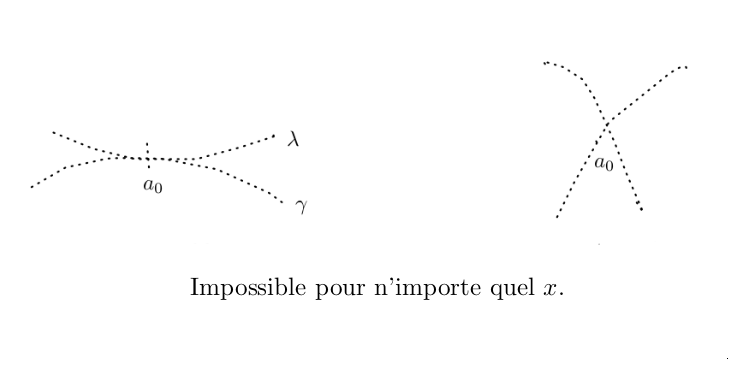
\includegraphics[scale=0.4]{figures/solution_max-corr.png}
  \caption{Aucune des deux  intersections  tangentes (\`a gauche) et transversales (\`a droite) n'est possible.}
  \label{solution_max}
\end{figure}



%%%%%%%%%%%%%%%%%%%%%%%
%%%%%%%%%%%%%%%%%%%%%%%
%%%%%%%19/10%%%%%%%%%%%
%%%%%%%%%%%%%%%%%%%%%%%
%%%%%%%%%%%%%%%%%%%%%%%
\subsubsection{Solutions maximales}

Pour toute courbe intégrale, on peut faire un changement de variable \(\tilde{t} = t+ t_0, \overline{\gamma}(t) = \gamma(t + t_0)\) pour lequel on obtient \(\tilde{\gamma}(0) = a_0\) (en principe on peut, sans perdre en généralité, supposer que \(t_0 = 0\) pour les systèmes autonomes d'EDO).

\'Etant donn\'e un champ de vecteur $X: U \to TU$, on consid\`ere  pour tout $x\in U$ l'ensemble de toutes les courbes int\'egrales passant par $x$ :
\[
 \mathcal{S}_x := \{(I, \gamma);\quad I\subset \R \,\, \text{intervalle ouvert},\,\, 0\in I,\,\, \gamma:I \to U \,\, \text{une courbe int\'egrale de}\,\, X \,\, \text{avec}\,\, \gamma(0)=x \}.
\]  En vue de l'unicit\'e des solutions on peut d\'efinir pour $X\in \mathcal{C}^1$ :
\begin{gather*}
I_x:= \bigcup_{(I, \gamma) \in  \mathcal{S}_x} I \\  \gamma_x : I_x \to \R \quad \gamma_x(t) := \gamma(t) \quad \text{si}\,\,  (I, \gamma) \in  \mathcal{S}_x\,\, \text{et} \,\, t\in I.
\end{gather*} Notons qu'il n'y a pas d'ambiguit\'e dans la d\'efinition de $\gamma_x$, et  la valeur de $\gamma_x(t)$ est unique pour tout choix de $(I, \gamma) \in  \mathcal{S}_x$ pour lequel $t\in I$: en effet si $(I,\gamma), (J, \lambda) \in  \mathcal{S}_x$, avec $t\in I, J$, on a
$0\in I, J$, $\gamma(0) = \lambda(0) = x$, et les deux applications $\gamma, \lambda$ \'etant les courbes int\'egrales on a par l'unicit\'e
\[
t\in I\cap J \implies \gamma(t) = \lambda(t).
\]

\begin{remark}
On observe que
\[
\forall (I, \gamma) \in  \mathcal{S}_x \quad \gamma = \gamma_{x\mid_I}.
\]
\end{remark}

Si on en a besoin, on va repr\'esenter l'intervalle maximale $I_x$ par ses bornes inf\'erieures et sup\'erieures \[I= ]\alpha_x, \omega_x[, \quad \alpha_x, \omega_x \in \R \cup \{\pm \infty\}, \alpha_x <
\omega_x.\]


\begin{remark}[Sur la taille de \(I_x\)]
  On définit \[M(x) = \sup _{\substack{i = 1, \dots, n\\j=1, \dots, n}} \left\vert \frac{\partial X ^{j} }{\partial x ^{i}} (x) \right\vert \]

  et

  \[b(x)= \sup \{ r \bg 0, B(x,r)\subset U \}.\]

  Alors il existe \(C \bg 0\) ne dépendant que de \(U\) et de $X$ (avec une dépendance explicite  aux travers les deux param\`etres expliqu\'es ci-dessous) tel que \[  |\alpha_x|, |\omega_x|  \geq C \left(\frac{b(x)}{\left\Vert X(w) \right\Vert }, M(x)\right).\]

 Ici, $C(a,b)$ est croissant en $a$ et d\'ecroissant en $b$. Alors \(\left\lvert I_x \right\rvert\) est plus large quand \(\displaystyle \frac{b(x)}{\left\Vert X(x) \right\Vert }\) est plus large ou bien quand \(M(x)\) est plus petit.
\end{remark}


\begin{exemple}
  On définit \(X : \mathbb{R}^2 \longrightarrow \mathbb{R}^2\) tel que \(X(x = (x^1, x^2)) = (x, x ^{\perp}) \in T_x \mathbb{R}^2\). On a

  \[\begin{bmatrix}
    0 & -1 \\
    1 & 0
  \end{bmatrix} \begin{bmatrix}
    x^1 \\
    x^2
  \end{bmatrix}\]

  et \(\gamma_x(t) = e^{At}x, I_x = (-\infty, \infty)\). On a \[\gamma_x(t) = (\cos(t)x^1 - \sin(t)x^2), \sin(t)x^1 + \cos(t)x^2 = \begin{bmatrix}
    \cos(t) & -\sin(t) \\
    \sin(t) & \cos(t)
  \end{bmatrix} \begin{bmatrix}
    x^1 \\
    x^2
  \end{bmatrix}.\]

  On calcule \(\gamma_x'(t) = (-\sin(t)x^1 - \cos(t)x^2, \cos(t)x^1 - \sin(t)x^2) = (\gamma_x(t))^{\perp}\). C'est une rotation d'angle \(t\) de point \(x\) autour du point 0.
\end{exemple}

\begin{remark}
  Si \(x = 0\), alors \(\gamma_0 = 0\).
\end{remark}

\begin{exemple}
  \(X : \mathbb{R}^2 \longrightarrow T \mathbb{R}^2\), \(X(x) = (x,-x) \in T_x \mathbb{R}^2\).

  On a \[-x = \begin{bmatrix}
    0 & -1 \\
    -1 & 0
  \end{bmatrix}x,\]

  \(\gamma_x(t) = e^{-t}x, I_x = (-\infty, \infty)\) et \(\gamma_x'(t) = - e^{-t}x = - \gamma_x(t)\) et \(\gamma_x(0)=x\).

  On a

  \begin{gather*}
    \lim_{t \to \infty} e^{-t}x = 0 \in \mathbb{R}^2 \\
    \lim_{t \to -\infty} \left\Vert e^{-t}x \right\Vert = +\infty.
  \end{gather*}
\end{exemple}




\subsubsection{Le flot d'un champ de vecteur}

Soit $U\subset \R^n$ un ouvert et \(X: U\to TU\) un champ de vecteur de r\'egularit\'e $\mathcal{C}^1$. On consid\`ere la famille des solutions maximales
$(I_x, \gamma_x)$, pour $x\in U$, et on met
\[
\widetilde U := \bigcup_{x\in U} I_x \times \{x\}.
\]

\begin{lemma}
$\widetilde U$ est un ensemble ouvert.
\end{lemma}

\begin{proof}[Démonstration, (détails en exercice)]


%%%%figures%%%%

On sait que \(b(x),\left\Vert X(x) \right\Vert \text{ et } M(x)\) sont continues en \(x\), alors on a :

\[\forall \varepsilon \bg 0, \exists \delta \bg 0, \text{ si } \left\Vert y-x \right\Vert \less \delta, \text{ alors } \left\lvert I_y \right\rvert \geq \left\lvert I_x \right\rvert - \varepsilon.\]

Comme \(\left\lvert I_x \right\rvert \bg 0\), on peut prendre \(\varepsilon = \displaystyle \frac{\left\lvert I_x \right\rvert}{2}\), on obtient \(\delta \bg 0\) tel que

\begin{equation}\label{sol_max1}
  \left\Vert y - x \right\Vert \less \delta \implies \left\lvert I_y \right\rvert \geq \left\lvert I_x \right\rvert - \frac{\left\lvert I_x \right\rvert}{2} = \frac{\left\lvert I_x \right\rvert}{2},
\end{equation}

ce qui implique que

\[\forall (t,x) \in \widetilde{U}, (t,x) \in \{ (s,y) \in \mathbb{R} \times \mathbb{R}^n \mid \left\Vert y-x \right\Vert \less \delta, s \in I_y \} \subseteq \widetilde{U}.\]


\emph{Indication :} l'argument sur la taille de l'intervalle d'existence devrait être transporté et basé sur \(t_0 = t\). Il faudra appliquer \ref{sol_max1} autour de \(t_0 = t\) et non à 0.


\end{proof}

\begin{definition}
  Soit $U  \subset\R^n$, un ouvert, $X : U \to TU$ un champ de vecteurs $\mathcal{C}^1$, et \(\gamma_x\)  la solution maximale sur \(I_x\) telle que \(\gamma_x(0) = x\). Le  \textbf{flot} \(\Phi : \widetilde{U}\longrightarrow U\) associé à \(X\) est d\'efini par
  \[\forall (t,x) \in \widetilde{U}, \Phi (t,x) \stackrel{\text{d\'ef}}=\gamma_x(t).\]

 Parfois il est pertinent d'utiliser la notation \(\Phi_t(x): =\Phi (t,x)\).
\end{definition}


\begin{thm}
Si \(X\) est de classe \(\mathcal{C}^r\), alors \(\Phi\) est de classe \(\mathcal{C}^r\).

\end{thm}

\marginnote{25-10-2023}

\begin{remark}
 Comme \((\gamma_x ^{i})'(t) = X ^{i}(\gamma_x(t)\)), il est facile de démontrer que \(\gamma_x\) dépend régulièrement en \(t\), et on gagne même une dérivée en $t$:
 \[X \in \mathcal{C}^r \implies \,\, \forall x\in U \,\, \gamma_x \in \mathcal{C}^{r+1} ;\] mais dans le th\'eor\`eme on réclame aussi la dépendance régulière de \(\gamma_x\) en \(x\).
 \end{remark}

\begin{remark}
  Pour \(t\) fixé, \(\Phi_t(x)\) est défini pour \[U_t := \{ x \in U \mid t \in I_x \}\] qui est un sous-ensemble ouvert de \(U\) (exercice). Donc \(\Phi_t : U_t \longrightarrow U \) est bien d\'efinie comme une application, et on a

  \[X \in \mathcal{C}^r \implies \phi_t \in \mathcal{C}^r.\] On a \(\Phi_0(x) = x\) et \(\Phi_0 = \operatorname{id}_U\).

 \end{remark}
%fig
\begin{prop}[sur la composition du flot]
  Si deux des trois valeurs \(\Phi_t(x)\), \(\Phi _{s}(\Phi_t(x))\) et \(\Phi _{s+t}(x)\) sont définies, alors la troisième aussi est définie et on a

  \[\Phi _{t+s}(x) = \Phi_s(\Phi_t(x)).\]
\end{prop}

\begin{proof}[Démonstration dans le cas où l'on sait que les trois valeurs sont définies]
  On va définir pour \(t\) fixé \(\eta(s) := \Phi_s(\Phi_t(x))\), et \(\Gamma(s) := \Phi _{s+t}(x)\). On a

  \begin{gather*}
    \eta(0) = \Phi_0(\Phi_t(x)) = \Phi_t(x)=y,
    \Gamma(0) = \Phi _{0+t}(x)= \Phi _{t}(x)=y.
  \end{gather*}

  De plus, son remarque que  \(\eta(s) = \gamma _{\Phi_t(x)}(s)\), alors

  \[\eta'(s) = \gamma' _{\Phi_t(x)}(s) = \sum_{i=1}^{n} X ^{i}(\gamma _{\Phi_t(x)}(s)) \frac{\partial  }{\partial x ^{i}}(\gamma _{\Phi _{t(x)}(s)})  =\sum_{i=1}^{n} X ^{i}(\eta(s)) \frac{\partial  }{\partial x ^{i}}(\eta(s)).\]

  Aussi \(\Gamma(s) = \gamma_x(s+t)\) et

  \begin{gather*}
    \Gamma'(s) = \frac{d}{ds}\gamma_x(s+t) = \gamma_x'(s+t) \underbrace{\frac{d}{ds}(s+t)}_{\equiv 1} = \gamma_x'(s+t) = \sum_{i=1}^{n} X ^{i}(\gamma_x(s+t)) \frac{\partial  }{\partial x ^{i}}(\gamma_x(s+t))\\
    = \sum_{i=1}^{n} X ^{i}(\Gamma(s)) \frac{\partial  }{\partial x ^{i}}(\Gamma(s)).
  \end{gather*}

  Donc \(\eta\) et \(\gamma\) tous les deux sont une solution (courbe intégrale) du champ de vecteurs \(X\) avec \(\eta(0) = \Gamma(0)=y\), donc ils devraient être égaux par unicité sur leur domaine commun de d\'efinition. Alors, pour tout \(s\) pour lequel les deux sont d\'efinis, on a \(\eta(s) = \Gamma(s)\), ce qui implique que \(\Phi _{t+s}(x) = \Phi_s(\Phi_t(x))\) quand les deux expressions sont d\'efinies.
\end{proof}

\begin{remark}
  Comme indiqu\'e dans la proposition, une observation plus fine démontre que si deux des trois acteurs \(\Phi_t(x), \Phi_s(\Phi_t(x)) \text{ et } \Phi _{t+s}(x)\) sont définis, alors le troisième aussi est défini et on a \(\Phi _{t+s}(x) = \Phi_s(\Phi_t(x))\).

  En particulier, si \(\Phi_t(x)\) est défini (i.e. \(t \in I_x\)), alors on a \(\Phi _{-t}(\Phi _{t}(x))\) est aussi défini et on a :

  \[x = \Phi _{-t}(\Phi _{t}(x)).\]

  Noter qu'on a pris \(s = -t\) et \(\Phi_0(x) = x\) est toujours défini.

  Donc \(\Phi_t(U_t) = U _{-t}\) et \(\Phi_t : U_t \longrightarrow U _{-t}\) est un difféomorphisme de régularité \(\mathcal{C}^r\) si \(X \in \mathcal{C}^r\).
\end{remark}

\begin{prop}
  Soit \(X\) un champ de vecteurs \(\mathcal{C}^1\) sur \(U\), \(K \subset U\) compact. On fixe \(T \in I_x\) et on suppose que pour tout \(t \in I_x\) tel que \(t \geq  T\), on a \(\Phi_t(x) \in K\), alors \(\omega_x = +\infty\) (donc \(I_x = (\alpha_x,+\infty)\)).

  (De même si \(\forall t \leq  T, \Phi_t(x) \in K\), alors \(I_x = (-\infty,\omega_x)\)).
\end{prop}

\begin{proof}
  Pour tout \(x \in U, \Phi_t(x) = \gamma_x(t)\) est défini pour un temps \(t\) qui  dépend de \(C\left(\frac{b(x)}{\left\Vert X(x) \right\Vert }, M(x)\right)\). Les arguments $b, \Vert X \Vert, M$ sont continues en \(x\) et positifs. Donc il existe \(c \bg 0\) dépendant de \(K\) tel que
   \[\forall x \in K\, \,C \left(\frac{b(x)}{\left\Vert X(x) \right\Vert }, M(x)\right) \geq c \bg 0.\]
  (Le minimum et maximums des fonctions continues  sur \(K\) sont atteints pour  les applications continues sur \(K\) compact). Alors pour tout \(x\in K,\,\, |\omega_x| \ge c\).

  \( |\omega_x| \ge c\) implique que pour \(x \in K, \Phi_t(x)\) est défini pour \(t \in \left[0, c\right[ \subset I_x\). On raisonne par contradiction. Supposons que \(\forall t \geq T, \Phi_t(x) \in K\) et \(\omega_x \less +\infty\), il existe alors \((t_k)\) une suite bornée telle que  \(T \le t_k \longrightarrow \omega_x \in \mathbb{R}, I_x = ]\alpha_x, \omega_x[\). On va prendre \(j\) assez grand tel que \(0   \less \omega_x - t _{k_j} \less  \frac c2 \).
 % Comme \(\{ \Phi _{t_k}(x)\}\subseteq K\) compact, alors il existe une sous suite \(\Phi _{t _{kj}}(x)\) qui converge dans \(K\) par la % compacité. Alors \(\Phi _{t _{k_j}} (x) \longrightarrow y \in K, t _{k_j}\longrightarrow \omega_x\).

Comme \(\Phi _{t _{k_j}}(x) \in K\), \(\Phi _{\frac c2}(\Phi _{t _{k_j}}(x))\) est défini. Aussi  \(\Phi _{t _{k_j}}(x)\) est défini. Alors par la  proposition sur composition du flot,  $t=  t_{k_j}, s=  \displaystyle \frac c2$

  \begin{gather*}
   \gamma_{x} (t_{k_j}  + \frac c2) = \Phi _{t_{k_j}  + \frac c2} (x) = \Phi _{t+s} (x)     \end{gather*}

  est défini.  Mais notons que $t_{k_j} + \frac c2 > \omega_x$ par le choix fait auparavant pour $j$. Ceci est une contradiction comme $\gamma_x(t)$ ne peut pas \^etre d\'efini pour $t>\omega_x$.
\end{proof}

\subsection{L'application tangente}

On suppose \(f : U \longrightarrow V\), \(U \subseteq \mathbb{R}^n\), \(V \subseteq \mathbb{R}^m\). On suppose que \(f\) est différentiable en \(a \in U\). On a \(Df(a) \in \mathscr{L}(\mathbb{R}^n, \mathbb{R}^m)\). On a \(d f(a) : T_a U \longrightarrow \mathbb{R}^m\) avec \(df(a)(a, \vec{v}) = Df(a)(\vec{v})\) avec \(\vec{v} \in \mathbb{R}^n\) et \((a,\vec{v}) \in T_a U\).

\begin{definition}
  L'application tangente \(T f: TU \longrightarrow T V\) est définie par :

  \[\forall (a,\vec{v}) \in  TU, \quad T f(a, \vec{v}) \stackrel{\text{d\'ef}}{=} (f(a), Df(a)(\vec{v})) \in T _{f(a)}V \subset T V.\]

\end{definition}
\begin{remark}

 \(T f _{\mid T_a U} : T_a U \longrightarrow T _{f(a)} V\) est linéaire.
\end{remark}

\begin{definition}
  On définit \(T_a f : = Tf _{\mid T_a U}\), avec

  \[T_a f(a, \vec{v}) = (f(a), D f(a)(\vec{v})).\]
\end{definition}

\begin{exemple}
  Soit \(i : U \longrightarrow \mathbb{R}^n\) une inclusion (injection canonique) avec \(i(x) =x\).  On prend \[T i : T U \longrightarrow T \mathbb{R}^n,\] et on a \(T i (x,\vec{v}) = (x, \vec{v})\), car \(D i(x)(\vec{v}) = \vec{v}\). Donc \(T i\) est l'inclusion de \(TU \) dans \(T \mathbb{R}^n\).
\end{exemple}

Lorsque \(m=1, f : U \longrightarrow \mathbb{R}\) et \(d_a f : T_a U \longrightarrow \mathbb{R}\) linéaire, donc \(d_a f \in (T_a U)^{*}\), donc \(df : U \longrightarrow T ^{*} U\). C'est un champ covariant.

Maintenant  notons que \(T f : T U \longrightarrow T \mathbb{R}\) et \(T_a f : \underbrace{T_a U}_{\{ a \} \times \mathbb{R}} \longrightarrow \{ f(a) \}\times \mathbb{R}\) linéaire. On ne peut plus dire que c'est une application de l'espace dual, mais elle admet quand même des propriétés intéressantes.

 \subsubsection{L'application tangente d'une composition}

\begin{prop}
  Si \(f : U \longrightarrow V\) est différentiable en \(x \in U\) et \(g : V \longrightarrow W\) est différentiable en \(f(x)\) et \(W \subseteq \mathbb{R}^{p}\). Alors \(T(g \circ f) = Tg \circ T f\).
\end{prop}

\begin{proof}[Vérification]
  \(T f: T U \longrightarrow T V, \forall (x,\vec{v}) \in T_x U \subseteq T U\), avec

  \[T f(x, \vec{v}) = (f(x), D f (x) (\vec{v})).\]

  On a de plus \(T g : T V \longrightarrow T W, \forall (y, \vec{w}) \in T_y V \subseteq T V\), avec

  \[Tg(y,\vec{w}) = (g(y), D g (y)(\vec{w})).\]

  Alors pour \(y:= f(x)\), et \( \vec w := Df(x(\vec v))\)

  \begin{gather*}
    T g \circ T f(x,\vec{v}) =  Tg(f(x), Df(x)(\vec{v})) = (g(f(x)),  Dg(f(x))\Big (Df(x)(\vec{v})\Big ))\\
    = ((g \circ f)(x), \underbrace{\Big (D g (f(x)) \circ D f(x)\Big )}_{D(g\circ f )(x)} (\vec{v}))= ((g \circ f)(x), D(g\circ f )(x)(\vec{v})) \\ =  T (g \circ f)(x, \vec{v}).
  \end{gather*}
\end{proof}

\begin{exemple}\label{dfoT} [Un cas particulier]
  \(U \stackrel{h}{\longrightarrow} V \stackrel{f}{\longrightarrow} \mathbb{R}\) et on a \(f \circ h : U \longrightarrow \mathbb{R}\). Alors \(d (f \circ h) : U \longrightarrow T ^{*} U\). On a aussi  \(T h : T U \longrightarrow T V\), \(d f : T V \longrightarrow \mathbb{R}\) et par une autre interpr\'etation \(d (f \circ h) : T U \longrightarrow \mathbb{R}\). On constate que
  \[
  d(f\circ h) = df \circ Th
  \]
\end{exemple}

\begin{proof}
  Il suffit d'observer que pour tout $f: V\to \R$, et par la d\'efinition de $df$
  \begin{equation}\label{df}
  Tf (y, \vec w) = (f(y), \underbrace{df(y, \vec w)}_{d_y f(\vec v)= df(y) (\vec w)}).
\end{equation} De m\^eme
  \[
  T(f\circ h) (x, \vec v) = (f\circ h(x) , d(f\circ h)(x, \vec v)).
  \] D'autre part \(T (f \circ h) =  Tf \circ Th\). On met $(y,\vec w) :=   Th(x, \vec v)$ dans \eqref{df}. Donc  en identifiant les deuxi\`emes composantes dans l'identit\'e \(T (f \circ h) =  Tf \circ Th\) on obtient
  \[
df(Th(x, \vec v)) = d(f\circ h)(x, \vec v).
  \] \end{proof}


 \subsubsection{Le pull-back et le push-forward des tenseurs}

\paragraph{Rappel} Si \(T : E \longrightarrow F\) linéaire, on rappelle que l'on peut définir \(\Omega ^{k}(T), \Omega _{l}(T), \dots\)

Alors pour les applications tangentes, $T_x f : T_x U \to T_{f(x)} V$ on a pour tout \(k,l\) :

\begin{gather*}
  \Omega ^{k}(T_x f) : \Omega ^{k}(T _{f(x)}V) \longrightarrow \Omega ^{k}(T _{x}U), \\
 \Omega _{l}(T_x f) : \Omega _{l}(T _{x}U) \longrightarrow \Omega _{l}(T _{f(x)}V), \\ \dots
\end{gather*}


\paragraph{Rappel}

On a dit que

\[T ^{k}U:= \bigcup _{x \in U} (\Omega ^{k}(T_x U)) .\]

\begin{definition}
Supposons que $U\subset \R^n$, $V\subset \R^m$, $f: U  \to V$ est {\bf injectif}.  On définit la fonction \(\Omega ^{k}f : T ^{k} V \longrightarrow T ^{k} U\), définie seulement pour tout élément \(\alpha \in T ^{k} V\) tel que \(\tau ^{k}(\alpha) \in f (U)\) (\( \tau ^{k}\) est la projection sur la \(k\)-ième coordonnée): \[\Omega ^{k}f(\alpha) \stackrel{\text{d\'ef}}{=} \Omega ^{k}(T_x f)(\alpha) \in \Omega^k(T_x U) \subset T^kU\] lorsque \(\alpha \in \Omega^{k}(T_y V)\), $y \in f(U)$, et $x\in U$ est le point unique pour lequel $y=f(x)$.

On peut aussi dire que $\Omega ^{k}f$ est d\'efinie comme  une application sur $T ^{k} W$, avec $W:=f(U)$.
\end{definition}

Pour \(\vec{v_1}, \dots, \vec{v_k} \in T _{x}U\), on a

\begin{gather*}
  \Omega ^{k} f(\alpha)(\overbrace{\vec{v_1}, \dots, \vec{v_k}}^{\in (T_x U)^{k}, k\text{ fois}}) = \alpha(T_x f(\vec{v_1}), \dots, T_x f(\vec{v_k}))).
\end{gather*}

%%%%fig%%%%%%

\begin{definition}
  On dit que \(\Omega ^{k}f(\alpha) \in \Omega ^{k}(T_x f) \subseteq T ^{k}U\), pour \(\alpha \in \Omega ^{k}(T_{f(x)} V) \subseteq T ^{k}V\) est le ``pull-back'' (le retiré) de \(\alpha\) sous l'action de l'application tangente \(T_x f : T_x U \longrightarrow T _{f(x)}V\).
\end{definition}

Par contre, pour tout \(\alpha \in \Omega_l(T_x U)\) et \(f : U \longrightarrow V\) différentiable en \(x \in U\), on a défini \[T_x f : T_x U \longrightarrow T _{f(x)} V,\] et on a alors

\[\Omega_l f \stackrel{\text{déf}}{=} \Omega_l (T_x f) : T_l U \longrightarrow T_l V,\]
avec  \(\Omega_l f (\alpha) \in \Omega_l(T _{f(x)} V)\subseteq T_l V\). \(\alpha\) étant un élément de \(\Omega_l(T_x U)\), il est une application \(l\)-linéaire sur \((T_x U)^{*}\) (contravariant). On cherche une application \(l\)-linéaire sur \((T _{f(x)} V)^{*}\).

Prenons donc un \(l\)-covecteur \(h_1, \dots, h_l \in T (T _{f(x)}V)^{*} = \mathscr{L}(T _{f(x)} V, \mathbb{R})\). Par la d\'efinition
\begin{gather*}
  \Omega_l f(\alpha)(h_1, \dots, h_l) = \alpha(h_1 \circ T_x f, h_2 \circ T_x f, \dots, h_l \circ T_x f).
\end{gather*}

Notez que si \(h_i \in (T _{f(x)}V)^{*}\), \(h_i : T _{f(x)}V \longrightarrow \mathbb{R}\) et \(T_x f : T_x U \longrightarrow T _{f(x)}V\), alors on obtient que \(h_i \circ T_x f : T_x U \longrightarrow \mathbb{R}\) linéaire, donc \(h_i \circ T_x f \in (T_x U)^{*}\).

%%%%fig%%%%%

On peut aussi interpréter \(\Omega_l f(\alpha)\) de la manière suivante : si \(T_x f : T_x U \longrightarrow T _{f(x)} V\) est donné, on a \((T_x f)^{*} : T^* _{f(x)}V \longrightarrow T^*_x U\) et

\begin{gather*}
  \Omega_l f(\alpha)(\underbrace{h_1, \dots, h_l}_{\in (T^*_{f(x) }V\times \dots \times T^* _{f(x)}V)}) = \alpha((T_x f)^{*}(h_1),\dots, (T_x f)^{*}(h_l)).
\end{gather*}

\begin{definition}
  Si \(\alpha \in \Omega_l (T_x U) \subseteq T_l U\), on dit que \(\Omega_l f(a)\) est le ``push-forward''(le poussé) de \(\alpha\) sous l'action de \(T_x f\).
\end{definition}

Chaque vecteur \(\vec{v} \in T_x U\) est un objet contravariant et il agit sur \((T_x U)^{*}\) par bidualité, i.e. \(T_x U \simeq (T_x U)^{**}\). Ici, \(l=1, \vec{v} \in T_x U\). Question : qu'est-ce \(\Omega_1 f(\vec{v})\) ?

\begin{prop}
Le push-forward d'un vecteur $\vec v \in TU$ est simplement $Tf(\vec v)$.
\end{prop}
\begin{proof}
  Prenons \(h \in (T _{f(x)}V)^{*}\),

  \begin{gather*}
    \Omega_1 f(\vec{v})(h) = \vec{v}(\Omega_1 (T_x f)(h)) = \vec{v}((T_x f)^{*}(h)) = \vec{v}(h \circ T_x f) = (h \circ T_x f)(\vec{v}).
  \end{gather*}



Donc on a vu que pour tout \(h \in (T _{f(x)} V)^{*}\), \(\underbrace{\Omega_1 f(\vec{v})}_{\in T _{f(x)V}}(\underbrace{h}_{\in (T _{f(x)}V)^{*}}) = h (T_x f(\vec{v}))\).

On a donc \(\forall h \in (T _{f(x)}V)^{*}, h(\Omega_1 f(\vec{v})) = h(T_x f (\vec{v}))\). Cela implique que \[\Omega_1 f(\vec{v}) = T_x f(\vec{v}),\quad  \forall \vec{v} \in T_x U.\]\end{proof}




  \begin{exo}
    Si \(\alpha \in \Lambda ^{k}(T _{f(x)}V)\) (\(\alpha\) est extérieur), alors \[\Lambda ^{k}f(\alpha) \stackrel{\text{déf}}{=}\Omega ^{k} f(\alpha) \in \Lambda ^{k}(T_x U).\]



    Si \(\alpha \in \Lambda _{l}(T_x U)\), \[\Lambda_l f(\alpha) \stackrel{\text{déf}}{=} \Omega_l f(\alpha) \in \Lambda_l(T _{f(x)} V).\]
  \end{exo}

\begin{remark}
Toutes d\'efinitions sont valides m\^eme pour $m\neq n$.
 \end{remark}

 \subsubsection{Le pull-back et le push-forward d'un champ tensoriel}

\begin{remark}\marginnote{{\fontencoding{U}\fontfamily{futs}\selectfont\char 66\relax}}
{\bf Avertissement :} Il faut distinguer entre les deux notions de tenseurs \(\alpha \in T^k_l U\) et le champ de tenseurs (i.e. le champ tensoriel) $\alpha : U \to T^k_l U$ (qui vient avec la propri\'et\'e \( \tau^k_l \circ \alpha =  \operatorname{id}_U\)).
\end{remark}

\begin{definition}
  Supposons que $U\subset \R^n$, $V\subset \R^m$ sont ouverts. Soit \(k\le 1\), \(f : U \longrightarrow V\) différentiable et \(\alpha : V \longrightarrow T ^{k} V\) {\bf un champ tensoriel} de type \((0,k)\) (une section de fibré tensoriel \(k\)-covariant), i.e. \(\forall y \in V, \alpha(y) \in T_y ^{k}V = \Omega ^{k}(T_y V)\).

  Le pull-back de \(\alpha\) sur \(U\), désigné par \(f ^{*}\alpha\) est un champ tensoriel de type \((0,k)\) sur \(U\), donc \(f ^{*}\alpha : U \longrightarrow T ^{k} U\).

  On met pour tout $x\in U$

  \[\underbrace{f ^{*}\alpha(x)}_{\in \Omega ^{k}(T_x U)} \stackrel{\text{déf}}{=} \Omega ^{k}(T_xf) ( \underbrace{\alpha(f(x))}_{\in \Omega ^{k}(T _{f(x) V})}).\]
\end{definition}
\begin{remark}
Donc pour chaque $x\in U$, $f ^{*}\alpha(x)$ est le pull-back de $\alpha(f(x))$ sur $T_xU$. On n'a pas besoin d'injectivit\'e pour $f$ ici, comme on d\'efinit un champ tensoriel $f ^{*}\alpha$, et pour chaque $x$,  la valeur $f(x)$ correspondante est bien d\'efinie.
\end{remark}

\begin{definition}
 Supposons que $U\subset \R^n$, $V\subset \R^m$, sont ouverts. Soit \(f : U \longrightarrow V\) différentiable, et \textbf{injectif},  et \(\beta : U \longrightarrow T _{l} U\) {\bf un champ tensoriel} de type \((l,0)\) (une section de fibré tensoriel \(l\)-contravariant) sur \(U\), i.e. \(\forall x \in U, \beta(x) \in \Omega_{l}(T_x U)\).
On définit alore  le ``push-forward'' de \(\beta\) désigné par \(f _{\sharp}\beta\). \(f _{\sharp}\beta\) est un champ tensoriel de type \((l,0)\) sur \(f(U)\subseteq V\) tel que
\[
\forall y = f(x) \in f(U), f _{\sharp}\beta(y) \stackrel{\text{déf}}{=} \Omega_l(T_xf)(\beta(x))\in \Omega _{l}(T_y V).
\]
\end{definition}

\begin{remark}
Donc pour chaque $y\in W=f(U)$, $f _{\sharp}\beta(y)$ est le push-forward de $\beta(x)$ sur $T_y W$. On a par contre besoin d'injectivit\'e pour $f$ ici, comme on d\'efinit un champ tensoriel $f _{\sharp}\beta : W \to T_lW$, et pour chaque $y \in W$,  il faut avoir une valeur unique de $x$ (de r\'ef\'erence) pour lequel $y=f(x)$, sinon il y a aurait une ambiguit\'e sur le pr\'eimage $x$ \`a choisir dans la d\'efinition.
\end{remark}

  \begin{exo}

  Si \(f : U \longrightarrow V, g : V \longrightarrow W\),    pour tout \(\alpha\) champ tensoriel de type \((0, k)\) sur \(W\),  on a
  \[(g \circ f)^{*} \alpha = f ^{*}(g ^{*}\alpha).\]


Si \(f\) et \(g\) sont injectives, pour tout \(\beta\) champ tensoriel de type \((l,0)\) sur \(U\),

  \[(g \circ f)_{\sharp}\beta = g _{\sharp}(f _{\sharp}\beta),\]

\end{exo}


 \subsubsection{Le push-forward d'un champ de vecteur sous un diff\'eomorphisme}
On suppose maintenant que \(U \subseteq \mathbb{R}^n, V \subseteq \mathbb{R}^n\) et \(h : U \longrightarrow V\) est un difféomorphisme \(\mathcal{C}^{\infty}\).

Si \(X\) est un champ de vecteurs sur \(U\), comme \(h\) est injective, alors \(h _{\sharp} X\) est un champ de vecteurs sur \(h(U)\) et  en plus on aura \(V=h(U)\). Donc $h_\sharp X$ est un champ de vecteur sur $V$. On aura

\[h _{\sharp}X(h(x)) = T_x h(X(x)) = Th \circ X(x).\]
Alors
\[h _{\sharp}X = Th \circ X \circ h ^{-1}.\]

Si \(h \in \mathcal{C}^r\), \(X \in \mathcal{C}^s\), on aura \(h _{\sharp} X \in \mathcal{C}^{\min(r-1, s)}\). Aussi
notez que \[h _{\sharp}X (y) = T h (X(h ^{-1}(y))) = (y,D h(h ^{-1}(y))\Big (X(h ^{-1}(y)\Big )).\]


%%%%fig%%%%%%


Avec les hypothèses \(h : U \longrightarrow U\) est un difféomorphisme de classe \(\mathcal{C}^\infty\), si \(X \in \mathcal{C}^1\) est un champ de vecteurs sur \(U\) avec le flot \(\Phi\), alors \(h _{\sharp}X\) est un champ de vecteurs sur \(V\) de régularité \(\mathcal{C}^1\).
\begin{prop}\label{flot-push-diff}
Soit $h:U\to V$ un diff\'epomorphisme $\mathcal{C}^\infty$ et $X : U \to TU$ un champ de vecteur de r\'egularit\'e $\mathcal{C}^1$. Dans ce cas-là, si \( \Phi, \Psi\) sont respectivement  les flots de $X$ et de \( Y= h _{\sharp}X \). Alors \(\Phi_t : \underbrace{U_t}_{\subseteq U} \longrightarrow \Phi_t(U_t)\) et \(\Psi : \underbrace{V_t}_{\subseteq V} \longrightarrow \Psi_t(V_t)\), tous les deux sont des difféomorphismes de régularité \(\mathcal{C}^1\). On a
\begin{gather*}
  h ^{-1}(V_t) = U_t \ (h(U_t) = V_t) \\
  h (\Phi_t(U_t)) = \Psi_t(V_t)
\end{gather*} (Donc il y a une consistance au niveau des domaines de définition). Finalement
\[
\Psi_t = h \circ \Phi _{t} \circ h ^{-1},
\]  c.\`a.d. le diagramme suivant est commutatif:
\begin{center}
\begin{tikzcd}[sep=1.5cm]
U_t \arrow[r, "\Phi_t"] \arrow[d, "h"]
& \Phi_t(U_t) \arrow[d, "h"] \\
V_t \arrow[r, "\Psi_t"]
& \Psi_t(V_t)
\end{tikzcd}
\end{center}

 \end{prop}
%fig1

\begin{figure}[h!]
  \centering
  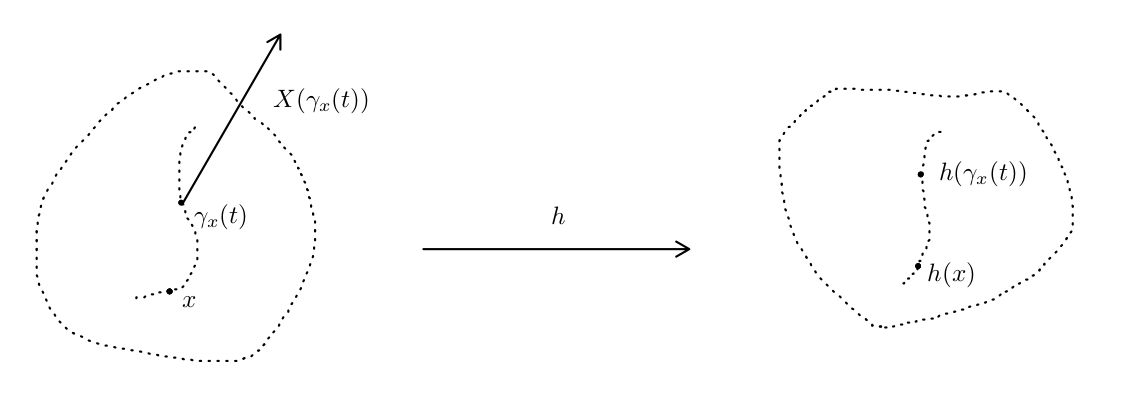
\includegraphics[scale=0.3]{figures/fig1-corr.png}
  \caption{Action d'un difféomorphisme sur le flot.}
  \label{fig1}
\end{figure}

\begin{proof}
  Soit $x\in U_t$ fix\'e. \(\Phi_t (x)  = \gamma_x(t)\) la courbe intégrale de \(X\). On d\'efinit pour $t\in I_x$
  \[
  \eta _{h(x)}(t) := h \circ \gamma_x(t) = h(\Phi_t(x)) \quad (\eta _{h(x)} = h \circ \gamma_x).
  \] On calcule \(\eta _{h(x)} = h(\gamma_x(0)) = h(x)\). Aussi

  \[T{\eta _{h(x)}} = T h \circ T \gamma_x.\]

  Alors,
    \begin{gather*}
    T{\eta _{h(x)}} \overbrace{\left( \frac{d}{dt}(t)\right) }^{(t,1)\in T_tI_x} = T h \circ {T{\gamma_x}\left(\frac{d}{dt}(t)\right)}  = Th(X (\gamma_x(t))) = h _{\sharp}X(h(\gamma_x(t))) = h _{\sharp}X(\eta _{h(x)}(t)),
  \end{gather*} o\`u on a utilis\'e  le fait que $\gamma_x$ est une courbe int\'egrale de $X$, i.e. ${T{\gamma_x}\left(\frac{d}{dt}(t)\right)} = X (\gamma_x(t))$.  On en d\'eduit

  \[\begin{cases}
    \eta _{h(x)}(0) = h(x) \\
    T{\eta _{h(x)}}\left(\frac{d}{dt}(t)\right) = (h _{\sharp}X)(\eta _{h(x)}(t)),
  \end{cases}\]

  donc \(\eta _{h(x)}\) est une courbe intégrale pour \(h _{\sharp}X\). Alors on d\'eduit que le flot $\Psi(\cdot ,x)$ est d\'efinit pour au moins $t\in I_x$ et

  \[\Psi(t,h(x)) = \eta _{h(x)}(t).\]

  Donc \[\Psi_t(h(x)) = h(\gamma_x(t)) = h(\Phi_t(x)).\]

 Notez  que $t\in I_x$ si et seulement si  $x\in U_t$. On a alors pour tout $x\in U_t$

  \begin{equation}
    \Psi_t \circ h (x) = h \circ \Phi_t (x).
  \end{equation}

Avec la consistence des domaines comme d\'ecrite dans la proposition, qui reste \`a \^etre d\'emontr\'ee (en exercice), on finit par conclure en composant avec $h^{-1}$ de deux cot\'es.
\[
   \Psi_t = h \circ \Phi_t \circ h^{-1}.
\]
\end{proof}

%%%%fig2%%%%%%%

\begin{figure}[h!]
  \centering
  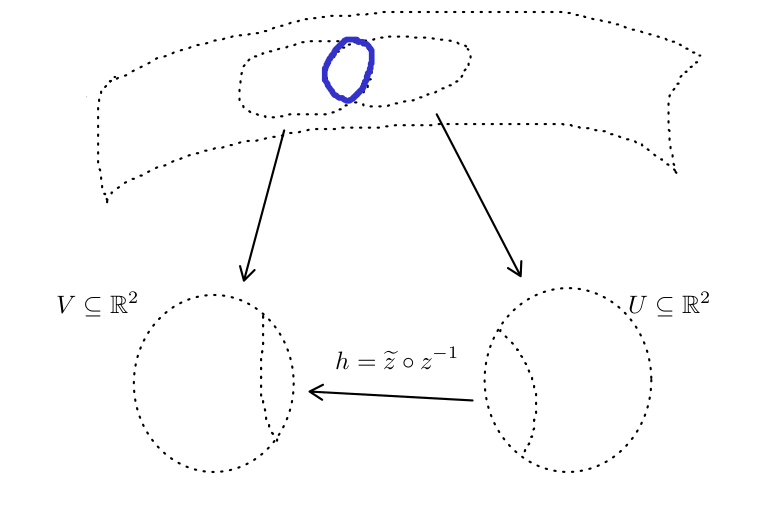
\includegraphics[scale=0.3]{figures/fig2-corr.png}
  \caption{}
  \label{fig2}
\end{figure}

\begin{figure}[h!]
  \centering
  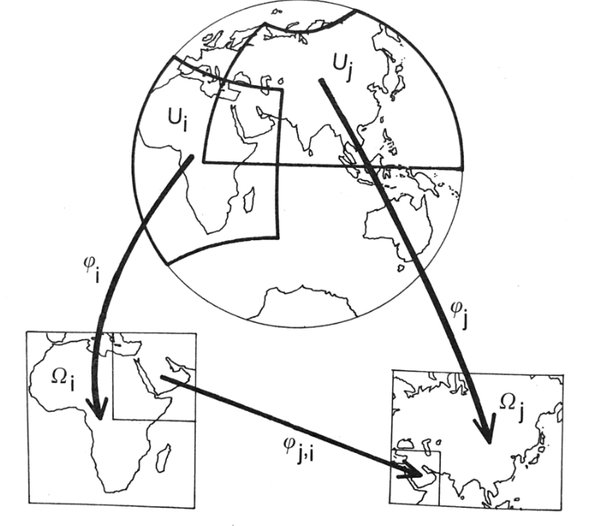
\includegraphics[scale=0.3]{figures/carte.jpeg}
  \caption{Une sphère n'est pas équivalente à \(\mathbb{R}^2\), mais une ``tranche'' de la sphère l'est. On appelle cela une ``carte''.}
  \label{}
\end{figure}

\begin{remark}
  Si \(X \in \mathcal{C}^{\infty}\), alors on a  \(\Phi_t : U_t \longrightarrow \Phi_t(U_t)\) est un difféomorphisme \(\mathcal{C}^\infty\). On peut, dans un cas spécial, utiliser \(h = \Phi_t, V=\Phi_t(U_t)\). Le flot \((\Phi)_{\sharp}X\) sur \(V\) est donnée par

  \begin{equation}\label{miracle}
    h \circ \Phi_t \circ h ^{-1} = \Phi_t \circ \Phi_t \circ (\Phi_t)^{-1} = \Phi_t.
  \end{equation}
\end{remark}

%%%%fig3%%%%%

\begin{figure}[h!]
  \centering
  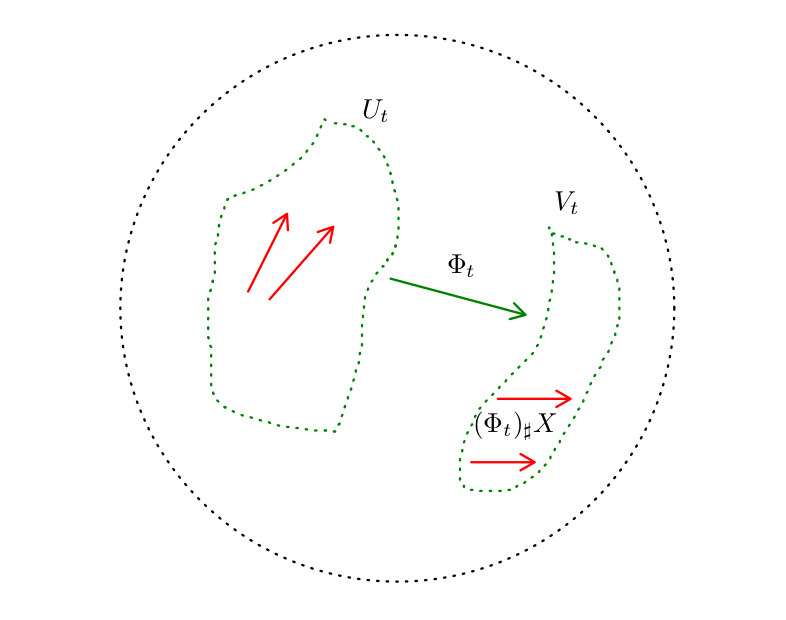
\includegraphics[scale=0.3]{figures/fig3.png}
  \caption{Le flot \(\Phi_t\)  du champs de vecteur $X$ laisse $X$ invariant \textcolor{red}{l'image \`a corriger}.}
  \label{}
\end{figure}

\begin{exo}
  \ref{miracle} implique que \((\Phi_t)_{\sharp}X(\Phi_t(x)) = X(\Phi_t(x))\).
\end{exo}

La forme la plus concise de cette formule de push-forward est :

\begin{equation*}
  (\Phi_t)_{\sharp}(X _{\mid U_t}) = X _{\mid \Phi_t(U_t)}.
\end{equation*}

\begin{exo}\label{flot-push}
Soient $U,V$ deux ouverts de $\R^n$, et $h: U\to V$ un diff\'eomorphisme $\mathcal{C}^\infty$.  Supposons que   $X:U\to TU,\,\,Y:V\to TV$, sont deux champs de vecteurs $\mathcal{C}^1$ avec les flots respectives $\Phi$ et $\Psi$, et qu'ils satisfont la propri\'et\'e suivante:
  \begin{equation*}
 \forall x\in U \,\, \exists \delta_x>0 \,\, \text{t.q.} \,\,   \forall  t\in ]-\delta_x, \delta_x[\quad   \Psi_t (x) = h \circ \Phi_t \circ h^{-1}(x).
  \end{equation*} D\'emontrer que $Y = h_\sharp X$.
\end{exo}

\subsubsection{Le th\'eor\`eme de bo\^ite de flot}

\begin{remark}
Supposons que $h: V \to W$ est un diff\'eomorphisme et que  le variable $y=h(x)$ est utilis\'e sur $W$, avec
\(W \subset\R^n :=\{ (y^1, \cdots, y^n); \,\, y^j\in \R\}\). On a le champ de vecteur sur $W$
\[
\displaystyle\frac{\partial  }{\partial y ^{1}}(y) = (y,e_1) : W \to TW.
\] S'il n'y a pas de confusion, et   \( W \) est consid\'er\'e comme un sous-ensemble de \[ \R^n :=\{ (x^1, \cdots, x^n); \,\, x^j\in \R\},\] (on a seulement chang\'e le nom du variable), on peut  d\'esigner ce champ de vecteur  avec \(\displaystyle\frac{\partial  }{\partial x ^{1}}\) aussi.
\end{remark}

\begin{thm}[``Ironing theorem'', ``Flow-box theorem'']
  Soient \(U \subseteq \mathbb{R}^n, X\) champ de vecteurs \(\mathcal{C}^\infty\) sur \(U\) et \(a \in U\) tel que \(X(a) \neq 0\). Alors il existe un ouvert \(V \subseteq U, a \in V\) et un difféomorphisme \(h : V \longrightarrow W \subseteq \mathbb{R}^n  :=\{ (y^1, \cdots, y^n); \,\, y^j\in \R\}\) tel que \[h _{\sharp}X _{\mid V} = \displaystyle\frac{\partial  }{\partial y^{1}}.\]

  En particulier, si \(\Phi\) est le flot de \(X\) et \(\Phi(t,x)\) est défini pour \(x \in V\), on a

  \[\Phi_t(x) = h ^{-1} \circ \Psi_t \circ h(x),\]

  où \(\Psi_t\) est le flot de \(\displaystyle \frac{\partial  }{\partial y ^{1}}\) sur $W$.
\end{thm}


%%%%%fig4%%%%%%

\begin{figure}[h!]
  \centering
  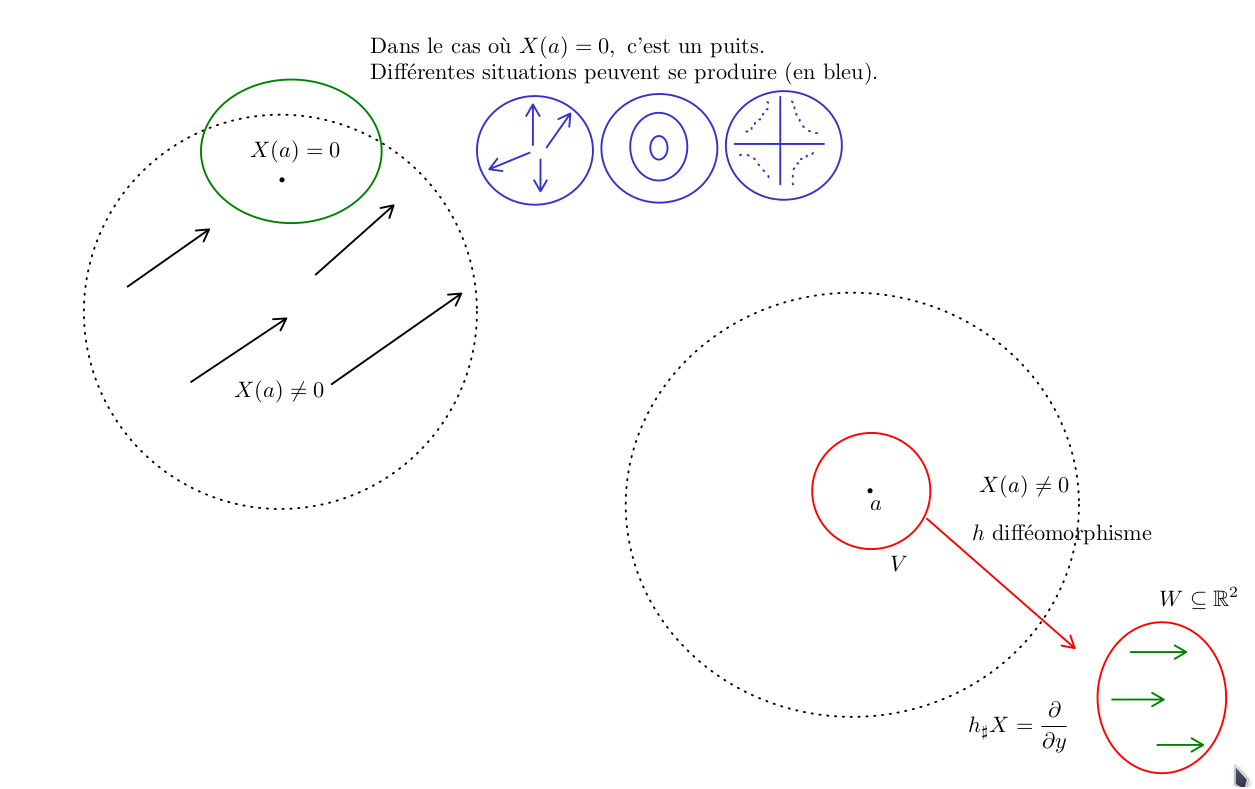
\includegraphics[scale=0.3]{figures/fig4.png}
  \caption{Les courbes intégrales vont être droites et plus ou moins parallèles. \textcolor{red}{la description \`a corriger: ce n'est pas que des puits}}
  \end{figure}

\begin{remark}
Comme  \(\displaystyle\frac{\partial  }{\partial y ^{1}}(y) = (y,e_1), \text{ alors on a }  \Psi_t(y) = y + t e_1\). Donc

  \begin{gather*}
    \Phi_t(x) = h ^{-1}(\Psi_t(h(x))) = h ^{-1}(y + t e_1).
  \end{gather*}
\end{remark}


\begin{proof}
Avec les rotations, les dilatations et les transformations, on peut supposer que \(a = 0, X(a) = \displaystyle \frac{\partial  }{\partial x ^{1}}(a)\). \begin{exo}

Si \(X(a) \neq 0\) est donné, on peut trouver une application \(h_0 : \mathbb{R}^n \longrightarrow \mathbb{R}^n\) affine \(h_0(x) = A x + \vec{b}, A \in \mathbb{R}^{n \times n}, \operatorname{det}(A) \neq 0\) telle que \(h_0(a) = 0\) et
\(((T _{h_0})_{\mid U})(X(a)) = \displaystyle \frac{\partial  }{\partial x ^{1}}(0)\).

{\it Indication:} L'existence de \(h_0\) qui vient du fait que \(\forall \vec{v} \in \mathbb{R}^n, \exists A \in \mathbb{R}^{n \times n}, A\) inversible telle que \(A \vec{v} = e_1\). Il faut fixer \(A\)   et ensuite définir \(h_0(x)=Ax - Aa\):
\end{exo}

\

{\bf Discussion:} Donc on peut supposer que \(0 \in U, X(0) = \frac{\partial  }{\partial x ^{1}}(0)\) (pourquoi?).

%%%%fig5%%%%%

\begin{figure}[h!]
  \centering
  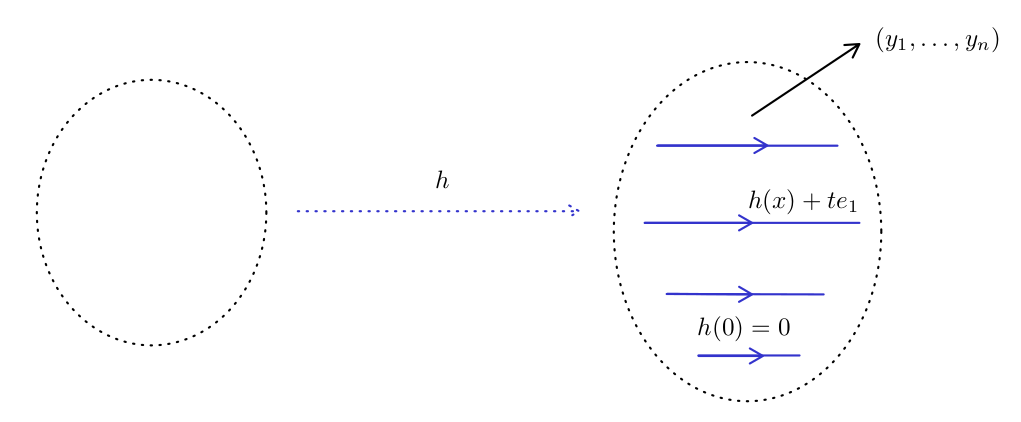
\includegraphics[scale=0.3]{figures/fig5.png}
  \caption{$\gamma_x(t) = \Phi_t(x)=h ^{-1}(h(x)+t e_1).$}
  \label{}
\end{figure}

Si on cherche $h$, on doit avoir pour $y= h(x)$

\begin{gather*}
  h ^{-1}(y^1+t, y^2, \dots, y^n) = \gamma_{h ^{-1}(y)}(t) = \Phi(t,h ^{-1}(y)) = \gamma_x(t) = \Phi(t,x).
\end{gather*}

Si \(x= (0, x^2, \dots, x^n)\), on va imposer que \(h(0, x^2, \dots, x^n) = (0, x^2, \dots, x^n)\). Alors il faut chercher \(h ^{-1}\) tel que

\[h ^{-1}(y^1, y^2, \dots, y^n) = h ^{-1}(0+\overbrace{y^1}^{t}, y^2, \dots, y^n) = \Phi(y^1, h ^{-1}(0,y^2, \dots, y^n)) = \Phi(\overbrace{y^1}^{t},  (0 , y^2, \dots, y^n)).\]

  On va alors définir (le candidat \(k\) pour \(h ^{-1}\)) \[k(y^1, \dots, y^n) := \Phi _{y^1}(0, y^2, \dots,y^n).\]

  On a bien sûr \(k(0) = \Phi_0(0) = 0\). \(k\) est défini pour \(y = (y^1, \dots, y^n)\) dans un voisinage ouvert de \(0 \in \mathbb{R}^n\) (exercice). On appelle ce voisinage \(\widetilde{W}\) avec \(0 \in \widetilde{W}, k : \widetilde{W} \longrightarrow U\). Si \(X \in \mathcal{C}^\infty\), alors \(\Phi \in \mathcal{C}^\infty\) et donc \(k \in \mathcal{C}^\infty\).

  %%%fig7%%%%

  \begin{figure}
    \centering
    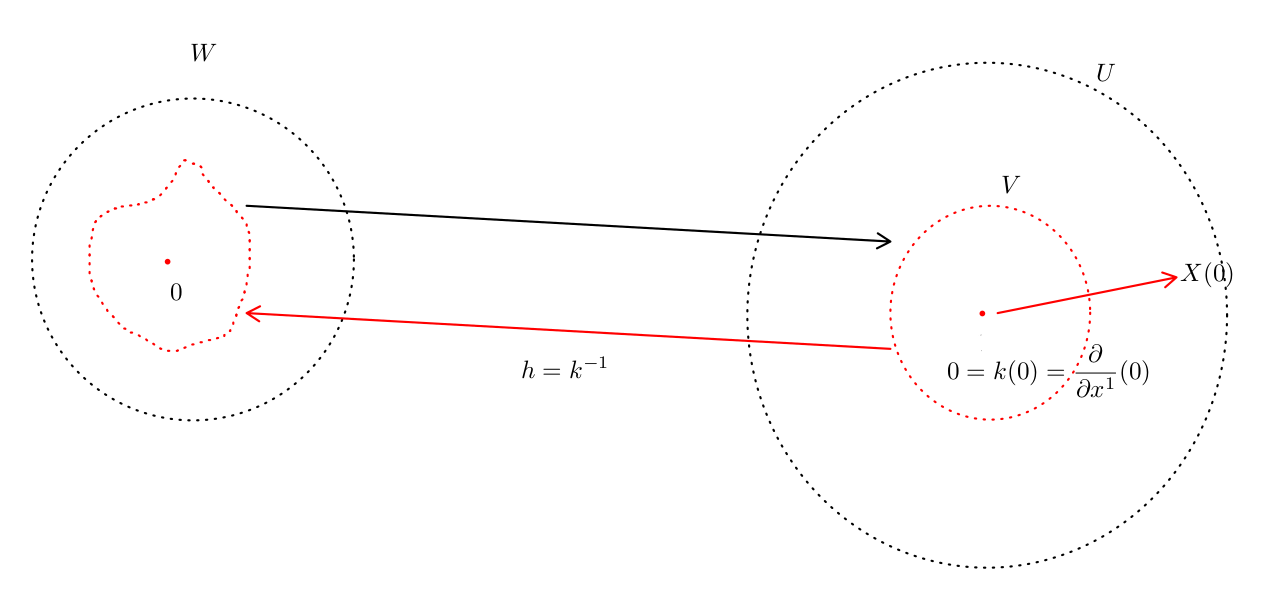
\includegraphics[scale=0.3]{figures/fig7.png}
    \caption{}
    \label{}
  \end{figure}

  On veut utiliser le théorème de l'application inverse. Il faut vérifier que \(D k(0)\) est inversible. On a

  \begin{gather*}
    Dk(0) = \left[ \frac{\partial k }{\partial y^{1}} \ \dots \ \frac{\partial k }{\partial y^{n}}  \right]_{\mid y=0}.    \end{gather*}
Pour calculer $\displaystyle \frac{\partial k}{\partial y^1}(0)$ il faut fixer $y^2 = \cdots= y^n=0$, donc

  \[k(y^1, 0, \dots, 0) = \Phi_{y^1} (0, 0, \cdots, 0) =  \gamma_{0}(y^1), \] et on obtient par le fait que \(\gamma_{0}\) est la courbe int\'egrale de $X$, avec $X(0) = (0, e_1)$:
  \[
  \displaystyle \frac{\partial k}{\partial y^1}(0)_{\mid y^1=0} = \gamma'_{0}(0)  =  e_1.
  \]  Pour calculer \(\displaystyle \frac{\partial k}{\partial y^j}(0), \,\, (j = 2, \dots,n)\)
 on a fixé \(y^1 = 0\), donc

  \[k(0, y^2, \dots, y^n) = \Phi_0(0, y^2, \dots, y^n) = (0, y^2, \dots, y^n), \]

  qui implique

  \[\frac{\partial k }{\partial y^{j}} (0) = (0,0, \dots, \underbrace{1}_{j}, \dots, 0) =e_j. \]

  Donc, en somme,
  \[
  Dk(0) = \left[ \frac{\partial k }{\partial y^{1}} \ \dots \ \frac{\partial k }{\partial y^{n}}  \right]_{\mid y=0} = \begin{bmatrix}
      1 & 0 & \dots & 0 \\
      0 & 1 & \dots & 0 \\
      \vdots & \vdots & \ddots & \vdots \\
      0 & 0 & \dots & 1
  \end{bmatrix}.
  \]
  et \(D k(0) = \operatorname{Id}_{n \times n}\) est inversible. Par le théorème de l'application inverse, il existe \(V \subset U\) ouvert avec \(0 \in V\), \(W \subseteq \widetilde{W}, 0 \in W\) tels que \(k: W \to V\) est inversible, avec l'inverse nomm\'e $h : V\to W$. On obtient alors que pour tout $y\in W$, on a $(0,y^2, \cdots, y^n) \in V_{y^1}$ et

  \[\Phi _{y^1}(0, y^2, \dots, y^n) = h ^{-1}(y^1, \dots, y^n).\]

 Comme \(k(0, y^2, \dots, y^n) = (0, y^2, \dots, y^n)\), on a \(h(0, y^2, \dots, y^n) = (0, y^2, \dots, y^n) \), et donc pour $x\in V$, $y= h(x)$, et $y+te_1 \in W$,

  \begin{gather*}
    h ^{-1}(y^1+t, y^2, \dots, y^n) = \Phi _{t+y^1}(0, y^2, \dots, y^n) = \Phi_t(\Phi _{y^1}(0, y^2, \dots, y^n)) = \Phi_t (h ^{-1}\underbrace{(y^1, \dots, y^n)}_{y})
  \end{gather*} Rappeler que \(\Psi_t(y) =  (y^1+t, y^2, \dots, y^n)\) est le flot du champ de vecteur \(\displaystyle \frac{\partial}{\partial y ^{1}}\) sur $W$,  alors on obtient
  \[
  h^{-1} \circ  \Psi_t (y) =  \Phi_t \circ h^{-1} (y) \implies      \Psi_t (h(x)) =  h(\Phi_t (x))  \implies    h(x) + te_1 =  h(\gamma_x(t))
  \] pour tout $y = h(x) \in W$ et $t\in \R$, pour lesquels $y+ te_1  \in W$.  En particulier, ces identit\'es  sont valides pour $|t|$ assez petit. Pour conclure, il suffit de d\'eriver en $t$ \`a $t=0$ \((\gamma_x(0) = x)\) pour obtenir
  \[
   e_1 =  Dh(x) \gamma'_x(0)
   \] qui, tenant compte du fait que $Th(x,\vec v) = (h(x), Dh(x) \vec v)$ et $T\gamma_x (\frac{d}{d t}(0))= (x, \gamma_x'(0)) = X(\gamma_x(0))$, implique
   \[
       \displaystyle \frac{\partial}{\partial y^1}(y) = (y,e_1) = Th \Big (T\gamma_x (\frac{d}{d t}(0))\Big ) = Th (X (x)) = h_\sharp X(h(x)) = h_\sharp X(y).
   \]
\end{proof}



\marginnote{26-10-2023}

\subsubsection{Le pull-back d'une métrique riemanienne}

Soit \(g\) la métrique riemanienne sur \(U\), \(g : U \longrightarrow T^2 U\) symétrique définie positive telle que \(\forall x \in U\), \(g(x)\) est un tenseur (0,2) (2-covariant) symétrique défini positif sur \(T_x U\). \(g(x) \in \Omega ^2(T_x U)\).

Pour un champ tensoriel covariant, c'est le retiré  sous une application qui a du sens. On considère \(V \subseteq \mathbb{R}^n\), \[u : V \longrightarrow U\] difféomorphisme \(\mathcal{C}^{\infty}\). Donc le retiré \(u ^{*}g\) est défini sur \(V\) comme un  champ tensoriel sur $V$:

\[u^*g : V \to T^2 V,\quad  \forall x \in V \quad u ^{*} g(x) \in  T^2_x V= \Omega ^2(T_x V)  \]

\begin{prop}
  Soit \(h := u ^{*} g\), alors \(h\) est une métrique riemanienne sur \(V\).
\end{prop}

\begin{proof}
  On sait déjà que \(h(x) \in \Omega ^2(T_x V), \forall x \in V\). Il faut démontrer que \(h(x)\) est un produit scalaire sur \(T_x U\).
Rappeler les d\'efinition d'applications tangente  $Tu: TV\to TU$ et d $u^*g$. On a
  \begin{enumerate}
    \item \(\forall \vec{v}, \vec{w} \in T_x V\),

    \begin{gather*}
    \begin{aligned}
      h(x)(\vec{v}, \vec{w}) & = u ^{*}g (x)(\vec{v}, \vec{w}) = g(u(x))(Tu (\vec{v}), Tu(\vec{w})) \\ &
      = g(u(x))(Tu(\vec{w}),Tu(\vec{v})) = u ^{*}g(x)(\vec{w}, \vec{v})=h(x)(\vec{w}, \vec{v}).
      \end{aligned}
    \end{gather*}

    \item Pour tout \(\vec{v} \in T_x V\), on a

    \begin{gather*}
      h(x)(\vec{v}, \vec{w}) = u ^{*}g(x)(\vec{v}, \vec{v}) = g(u(x))(T u(\vec{v}), Tu(\vec{v})) \geq 0.
    \end{gather*}

    De plus, on a

    \begin{gather*}
      h(x)(\vec{v}, \vec{v})=0 \iff g(u(x))(T u (\vec{v}), T u (\vec{v})) = 0 \iff T u(\vec{v}) \iff \vec{v} = 0.
    \end{gather*}

    \begin{remark}
      Si \(u : U \longrightarrow V\) difféomorphisme, on a pour tout \(x \in V\), \(T_x u : T_x V \longrightarrow T_x U\) est une application linéaire inversible. En effet,

      \begin{gather*}
        T u \circ T u ^{-1} = T (u \circ u ^{-1}) = T (\operatorname{id}_U) = \operatorname{id}_{TU} \\
        T u ^{-1} \circ T u = T (u ^{-1} \circ u) = T(\operatorname{id}_V) = \operatorname{id}_{TV}.
      \end{gather*}
    \end{remark}
  \end{enumerate}
\end{proof}



\begin{exo}
  Montrer que si \(u : V \longrightarrow U\) difféomorphisme \(\mathcal{C}^{\infty}\) et \(g\) métrique riemannienne  sur \(U\), alors

  \begin{enumerate}
    \item \(h = u ^{*}g\) implique que \(\forall x\in U, \,\,  \forall \vec{v}, \vec{w} \in T_x U\) :

    \begin{gather}
      \left\Vert \vec{v} \right\Vert _{h} = \left\Vert T u(\vec{v}) \right\Vert _{g} \\
      \sphericalangle (\vec{v}, \vec{w})_h = \sphericalangle(T u(\vec{v}), T u (\vec{w}))_g.
    \end{gather}

    \item Pour toute m\'etrique riemannienne $h$ sur $V$ \[\forall x\in U, \,\, \forall \vec{v} \in T_x U, \left\Vert \vec{v} \right\Vert _{h} = \left\Vert T u(\vec{v}) \right\Vert_g  \implies h = u ^{*}g.\]
  \end{enumerate}
\end{exo}

\begin{exo}
  Soit
  \[ \mathscr{M} \stackrel {\text{d\'ef}}{=} \left \{ (U,g) \mid U \subseteq \mathbb{R}^n \text{ ouvert},  \,\, g \text{ métrique riemanienne sur } U\right \}.
  \]  Pour tout \((U,g), (V,h) \in U\), on définit la relation suivante :

  \[(U,g) \sim (V,h) \iff \exists u : V \longrightarrow U \text{ difféomorphisme } \mathcal{C}^{\infty} \text{ tel que } h = u ^{*}g.\]

  D\'emontrer que $\sim$ est une relation d'\'equivalence sur $\mathscr{M}$.
\end{exo}


\subsubsection{Longueur des courbes sous le  pull-back de la m\'etrique riemannienne}

\begin{thm}
  Soit \(U, V \subseteq \mathbb{R}^n\), avec \(g, h\) deux  métrique riemanienne  continues sur respectivement \(U\) et \(V\). On suppose que \(u : V \longrightarrow U\) est un difféomorphisme \(\mathcal{C}^{\infty}\).  Consi\`erons les trois conditions suivantes :

  \begin{enumerate}

       \item  \label{rieman-3}\(h = u ^{*}g\).
   \item \label{rieman-2} Pour toute courbe \(\gamma : [a,b] \longrightarrow V\), \(L_h(\gamma) = L_g(u \circ \gamma)\).
     \item \label{rieman-1} Pour tous \(x,y \in V\), \(d_h(x,y) = d_g(u(x),u(y))\).
       \end{enumerate}

Alors,  \ref{rieman-3} et  \ref{rieman-2} sont \'equivalentes. En plus, elles impliquent \ref{rieman-1} et  au cas o\`u $g$ and $h$ sont de classe $\mathcal{C}^2$, elles sont  \'equivalentes avec  \ref{rieman-1}
\end{thm}


\begin{proof}
  Il est claire que \ref{rieman-2} implique \ref{rieman-1}. Pour le moment, on va suspendre la démonstration de la suffisance de \ref{rieman-1} dans le cas o\`u $g, h\in \mathcal{C}^2$.  On  se rappelle que

  \begin{gather*}
    L_h(\gamma) := \int_{a}^{b} h(\gamma(t))(T \gamma \left(\frac{d}{dt}(t)\right), T \gamma \left(\frac{d}{dt}(t)\right))dt \\
\Big (    = \int_{a}^{b} \sum_{i,j}^{} H _{ij}(\gamma(t))(\gamma ^{j})'(t) (\gamma ^{i})'(t)dt = \int_{a}^{b} \langle \gamma'(t) \mid H (\gamma(t)) \mid \gamma'(t) \rangle dt. \Big )
  \end{gather*}

  %%%%suite de démo rieman%%%%%

On va démontrer d'abord que \ref{rieman-3} implique \ref{rieman-2}. Soit $\gamma :[a,b] \to V$ une courbe diff\'erentiable.  Rappeler que \(T \gamma : T I \longrightarrow T V, T u : T V \longrightarrow T U\), et  que l'application tangante d'une composition est la composition des applications tangentes.  Par \ref{rieman-3}  on a  \(h = u ^{*}g\),   et alors

  \begin{gather*}
    L_h(\gamma) = \int_{a}^{b} h(\gamma(t)) \left(T \gamma \left(\frac{d}{dt}(t)\right), T \gamma \left(\frac{d}{dt}(t)\right)\right) dt \\
    = \int_{a}^{b} u ^{*}g(\gamma(t))\left(T \gamma \left(\frac{d}{dt}(t)\right), T \gamma \left(\frac{d}{dt}(t)\right)\right) \\
    = \int_{a}^{b} g(u(\gamma(t))) (T u \Big (T \gamma \left(\frac{d}{dt}(t)\right)  \Big ), T u \left(T \gamma \left(\frac{d}{dt}(t)\right)\right))  dt\\
    = \int_{a}^{b} g (u \circ \gamma(t)) \left(T u \circ T \gamma \left(\frac{d}{dt}(t)\right), T u \circ T \gamma \left(\frac{d}{dt}(t)\right)\right)  \\
    = \int_{a}^{b} g(u \circ \gamma(t)) \left(T (u \circ \gamma) \left(\frac{d}{dt}(t)\right), T(u \circ \gamma)\left(\frac{d}{dt}(t)\right)\right)  = L_g(u \circ \gamma),
  \end{gather*} ce qui d\'emontre \ref{rieman-2}.




  Pour d\'emontrere la r\'eciproque, \ref{rieman-2} $\implies$ \ref{rieman-3}, on suppose \ref{rieman-2}.  Par le calcul qu'on vient de faire,
  \[\forall \gamma \in \mathcal{C}^1, \gamma : [a,b] \longrightarrow V \quad L_g (u \circ \gamma) = L_h(\gamma)\] implique que

  \begin{gather*}
  \begin{aligned}
 \forall \gamma \in \mathcal{C}^1, \gamma : [a,b] \longrightarrow V\quad  &  \int_{a}^{b} u ^{*}g(\gamma(t))\left(T \gamma \left(\frac{d}{dt}(t)\right), T \gamma \left(\frac{d}{dt}(t)\right)\right) dt \\ &
    = \int_{a}^{b} h (\gamma(t)) \left(T \gamma \left(\frac{d}{dt}(t)\right), T \gamma \left(\frac{d}{dt}(t)\right)\right) dt.
 \end{aligned}
  \end{gather*}

  Soit \(x \in V, \vec{v} \in T_x V\), avec \(\vec{v}=(x, \underbrace{\mid \vec{v} \rangle}_{\in \mathbb{R}^n})\). On pose
  \[  \gamma : [-\varepsilon, \varepsilon] \longrightarrow \R^n, \quad \gamma(t) = x + t \mid \vec{v} \rangle,\] et on note qu'il existe \(\varepsilon \bg 0\) tel que \(\gamma([-\varepsilon, \varepsilon]) \subseteq V\).
  On pose \(a = -\varepsilon,b=s \in (-\varepsilon,\varepsilon)\).  Alors
  \begin{gather*}
    \int_{a}^{s} u ^{*}g(\gamma(t)) \left(T \gamma \left(\frac{d}{dt}(t)\right), T \gamma \left(\frac{d}{dt}(t)\right)\right) dt = \int_{a}^{s} h(\gamma(t)) \left(T \gamma \left(\frac{d}{dt}(t)\right), T \gamma \left(\frac{d}{dt}(t)\right)\right) dt.
  \end{gather*}

  Les int\'egrandes sont continues, donc par le th\'eor\`eme fondamental du  calcul infinit\'esimal, et en d\'erivant les deux int\'egrales en $s$, on obtient que pour tout $t\in ]-\varepsilon, \varepsilon[$, es deux int\'egrandes sont \'egales:

  \begin{gather*}
 u ^{*}g(\gamma(t)) \left(T \gamma \left(\frac{d}{dt}(t)\right), T \gamma \left(\frac{d}{dt}(t)\right) \right )= h(\gamma(t)) \left(T \gamma \left(\frac{d}{dt}(t)\right), T \gamma \left(\frac{d}{dt}(t)\right)\right).
  \end{gather*}


  On évalue en \(t = 0\). On a \(\gamma(0) = x + 0 \cdot \mid \vec{v} \rangle = x\) , \(\gamma'(t) = \mid \vec{v}\rangle \), et on obtient alors :

  \begin{gather*}
    T \gamma \left(\frac{d}{dt}(t)\right)_{\mid t=0} = (\gamma(0), \gamma'(0)) = (x,  \mid \vec{v} \rangle)
  \end{gather*}

  ce qui implique que

  \begin{gather*}
    u ^{*}g(x)((x,\mid \vec{v} \rangle), (x, \mid \vec{v} \rangle)) = h(x)((x,\mid \vec{v} \rangle), (x,\mid \vec{v} \rangle)).
  \end{gather*}

Alors on a \'etabli que
  \begin{gather*}
\forall \vec v \in T_x V\quad     u ^{*}g(x)(\vec{v},\vec{v}) = h(x)(\vec{v}, \vec{v}).
  \end{gather*} On a alors pour tout $\vec v,w\in T_xV$
  \[
  u ^{*}g(x)(\vec{v} +\vec {w},\vec{v}+\vec{w}) = h(x)(\vec{v}+ \vec{w}, \vec{v} +\vec {w}).
\] Utilisant la bi-lin\'earit\'e et la sym\'etrie on obtient
\begin{gather*}
  u ^{*}g(x)(\vec{v},\vec{v}) +   2 u ^{*}g(x)(\vec{v},\vec{w}) +   u ^{*}g(x)(\vec{w},\vec{w}) \\ =
    h(x)(\vec{v},\vec{v}) +   2 h(x) (\vec{v},\vec{w}) +  h(x)(\vec{w},\vec{w})
\end{gather*}  et on donc conclut  avec
  \[
   \forall \vec v, \vec w \in T_x V\quad     u ^{*}g(x)(\vec{v},\vec{w}) = h(x)(\vec{v}, \vec{w}),
   \] i.e. $u^*g =h$.
\end{proof}



\begin{definition}
  Soit \(U, V \subseteq \mathbb{R}^n\), avec \(g, h\) deux  métrique riemanienne  continues sur respectivement \(U\) et \(V\), et   \(u : V \longrightarrow U\) diff\'eomorphisme $\mathcal{C}^1$.  Quand $h= u^*g$, on dit que $u$ est une {\it isom\'etrie}  (ou bien une {\it \'equivalence isom\'etrique}) entre les deux vari\'et\'es riemanniennes \((U,g)\) et \((V,h)\). Si un tel $u$ existe, on dit que  \((U,g)\) et \((V,h)\) sont isom\'etriques.
\end{definition}


\subsubsection{Calcul pour les matrices \(G\) et \(H\) quand $h= u^*g$.}

On a

\begin{gather*}
  h= \sum_{i,j=1}^{n} h _{ij}d x^{i}\otimes d x^{j},  g = \sum_{i,j=1}^{n} g _{ij}d y ^{i} \otimes d y ^{j}, (y^1, \dots, y^n) \in U.
\end{gather*}

Si \(h = u ^{*} g\), quelle est la relation entre les matrices \(G\) et \(H\) ?

\medskip

Soit \(x \in V,  \vec{v}, \vec{w} \in T_x V\), avec \(\vec{v} = (x,\mid \vec{v} \rangle), \vec{w} = (x, \mid \vec{w} \rangle)\), avec

\[\vec{v}  = \sum_{j}^{} v ^{j} \frac{\partial  }{\partial x ^{j}}(x)\]

et

\[\mid \vec{v} \rangle = \begin{bmatrix}
  v ^{1} \\
  \vdots \\
  v ^{n}
\end{bmatrix}.\]

On a
\begin{gather*}
\begin{aligned}
h = u ^{*}g \iff \forall x \in V, \forall \vec{v}, \vec{w} \in T_x V,\quad  h(x)(\vec{v}, \vec{w}) & = g(u(x))(T u (\vec{v}), T u (\vec{w})) \\ &  \end{aligned}
\end{gather*}
qui implique
\begin{gather*}
\begin{aligned}
h = u ^{*}g \iff \forall x \in V, \forall \mid \vec{v},\rangle \mid  \vec{w} \rangle \in \R^n ,\quad  \langle \vec{v} \mid H_x \mid  \vec{w}\rangle  = \langle D u(x)\vec{v} \mid G_{u(x)} \mid D u(x)\vec{w}\rangle.
\end{aligned}
\end{gather*}

On prend maintenant \(\mid \vec{v} \rangle = e_i \in \mathbb{R}^n, \mid \vec{w} \rangle = e_j \in \mathbb{R}^n\). Alors on a :

\begin{gather}\label{machin}
h _{ij}(x) =  \underbrace{\langle e_i \mid  H_x \mid e_j \rangle}_{e_i \cdot H e_j} =  \langle D u(x)e_i \mid G_{u(x)} \mid D u(x)e_j\rangle.
\end{gather}

Or \(D u(x)e_i\), c'est la \(i\)-ième colonne de \(  D u(x) = \begin{bmatrix} \displaystyle \frac{\partial u }{\partial x ^{1}}(x) & \displaystyle \cdots & \displaystyle \frac{\partial u }{\partial x ^{n}}(x)  \end{bmatrix} \), ce qui donne

\begin{gather*}
  \ref{machin} \implies h_{ij}(x) = \left\langle \frac{\partial u }{\partial x ^{i}}(x) \mid G_{u(x)} \mid \frac{\partial u }{\partial x ^{j}}(x)   \right\rangle.
\end{gather*}

On en d\'eduit alors

\[H_x = \prescript{t}{}\!\!Du(x) G_{u(x)}Du(x).\]

La r\'eciproque peut \^etre \'etablie suivant le m\^mem calcul.  On vient de d\'emontrer que
\begin{prop}\label{pull-back-metrics}
  Supposons que \(u: V\to U\) est un difféomorphisme \(\mathcal{C}^{\infty}\), et \(h,g\) sont duex m\'etrique riemannienne   sur respectivement \(V, U\). Si \[h = \displaystyle \sum_{i,j} h _{ij}d x^{i} \otimes d x^{j} \text{ sur } V,\quad  g = \displaystyle \sum_{i,j}^{} g _{ij} d y ^{i}\otimes d y ^{j} \text{ sur } U\] alors on a \[h = u ^{*}g \iff \forall x \in V, H_x =  \prescript{t}{}\!Du(x) G_{u(x)}Du(x).\]
\end{prop}

\begin{exemple}
  On prend \(u : \mathbb{R}^2 \longrightarrow \mathbb{R}^2\) et

  \[u(x,y) = \begin{bmatrix}
    x+y \\
    y
  \end{bmatrix}.\]

  On a \(Du(x,y) = \begin{bmatrix}
    1 & 1 \\
    0 & 1
  \end{bmatrix}\). \(u\) est un difféomorphisme \(\mathcal{C}^{\infty}\). On pose \(G = \begin{bmatrix}
    1 & 0 \\
    0 & 1
  \end{bmatrix}\) (avec \(g\) la métrique euclidienne sur \(\mathbb{R}^n\)).

  Alors on a

  \begin{gather*}
    H =    \prescript{t}{}{\begin{bmatrix}
      1 & 1   \\
      0 & 1
  \end{bmatrix}} \begin{bmatrix}
    1 & 0 \\
    0 & 1
\end{bmatrix}\begin{bmatrix}
  1 & 1 \\
  0 & 1
\end{bmatrix} = \begin{bmatrix}
  1 & 0 \\
  1 & 1
\end{bmatrix} \begin{bmatrix}
1 & 0 \\
0 & 1
\end{bmatrix}\begin{bmatrix}
1 & 1 \\
0 & 1
\end{bmatrix} = \begin{bmatrix}
  1 & 1 \\
  1 & 2
\end{bmatrix}
  \end{gather*}

  Ainsi \(\forall \mid \vec{v} \rangle, \mid \vec{w} \rangle \in \mathbb{R}^2\), on a

  \begin{gather*}
    \langle \vec{v} \mid \vec{w} \rangle_{H} = v ^{1} w ^{1} + v ^1 w ^2 + w ^2 v ^{1} + 2 v ^2 w ^2
  \end{gather*}

  et

  \[\left\Vert \vec{v} \right\Vert _{H}^2 = (v ^{1})^2 + 2 v ^{1}v ^2 + 2(v ^2)^2 = (v ^{1} + v ^2)^2+(v ^2)^2.\]

  On obtient \(h = dx \otimes dx + dx \otimes dy + dy \otimes dx + 2 dy \otimes dy\).
\end{exemple}

\begin{corollary}
Soit \(g_{eu}\) la métrique euclidienne standard sur \(U \subseteq \mathbb{R}^n\): \[G_{eu} = I _{n \times n}, \quad g_{eu} = \sum_{i=1}^{n}d x^{i} \otimes d x^{i}\] et  soit \(u : V \longrightarrow U\)  un  difféomorphisme \(\mathcal{C}^{\infty}\).

  Alors si \(h= u ^{*} g, h = \sum_{i,j=1}^{n} h _{ij}d x^{i}\otimes d x^{j}, H = [h _{ij}] \in \mathbb{R}^{n \times n}\), on a

  \[H = (\prescript{t}{}\!D u) D u.\]
\end{corollary}

\begin{remark}
  \(\forall A \in \mathbb{R}^{n \times n}, \forall   \vec{v}  ,   \vec{w}  \in \mathbb{R}^n\), si \(H = \prescript{t}{}\!A A\), on a

  \begin{gather*}
    \langle \vec{v} \mid H \mid \vec{w} \rangle = \langle \vec{v}\mid \prescript{t}{}\!A A \mid \vec{w} \rangle = \langle A \vec{v} \mid A \, \vec{w} \rangle = \vec{v} \cdot ( \prescript{t}{}\!A A \vec{w}) = A \vec{v} \cdot A \vec{w}.
  \end{gather*}

  De plus, on a

  \[\langle \vec{v} \mid H \mid \vec{v} \rangle = \langle A \vec{v} \mid A \vec{v} \rangle   = \left\Vert A \vec{v} \right\Vert ^2,\]  qui est le carr\'e de  la norme euclidienne de $A\vec v$.
\end{remark}

\begin{exemple}
  Soit \(V = \{ (x,y) \in \mathbb{R}^2 \mid y \bg 0 \}\), \(u(x,y) = (x + y ^2, y)\). Notez que $u:V\to V$ est un diff\'eomprphisme. On met $h:= u^*g_{eu}$.  On  calcule \[Du (x,y)= \begin{bmatrix}
    1 & 2 y \\
    0 & 1
  \end{bmatrix},\] et on  obtient alors

  \begin{gather*}
    H = \prescript{t}{} \!Du Du = \begin{bmatrix}
      1 & 2y \\
      2 y & 1 + 4y ^2
  \end{bmatrix}.
\end{gather*}

  Alors \[h = dx \otimes dx + 2 y \,dx \otimes dy + 2 y\, dy \otimes dx + (1+ 4y ^2)\, dy \otimes dy.\]


On \'etudie les pr\'e-images sous $u$ des g\'eod\'esies de $g_{eu}$, qui sont les lignes droites dans $U=u(V)= V$.
  Si \(u(x,y) = (x', y')\), alors on a \(x+ y ^2 = x', y=y'\), donc \(x = x' - y ^2 = x' - (y')^2\). On obtient donc

  \[u ^{-1}(x',y') = (x' - (y')^2,y').\]

 Le pr\'e-image sous $u$ de la ligne droite \(x' \equiv \text{constante}\) et \(y\) arbitraire (paramètr\'e par  \(y=t\)), est la courbe dans \(V\) de la forme \((c -t ^2, t), t \bg 0\), qui est la partie sup\'erieure \((y>0)\) du parabole \(x= c-y^2\).



  Sinon, \(y' = ax'+b, t=x', y'=at+b\), donc la courbe géodésique correspondant pour \((V,h)\) est

  \[(t -(at+b)^2, \overbrace{at+b}^{y} ).\]

  \begin{itemize}
    \item [$\star$] Si \(a \neq 0\), on  a \(y = at+b\), \(t = \displaystyle\frac{y-b}{a}, x = \displaystyle\frac{y-b}{a} - y ^2 = -y ^2+ \displaystyle\frac{y}{a} - \displaystyle\frac{b}{a}\); donc la courbe pr\'e-image est la partie sup\'erieure \((y>0)\) d'une parabole.
    \item [$\star$] Si \(a= 0\), \(y'=  b \bg 0, x' = t\) (paramètre), la courbe dans \((V,h)\) est \((t-b^2,b)\), qui est aussi une ligne horisontale.
  \end{itemize}
\end{exemple}

%%%%fig10%%%%%%

\begin{figure}[h!]
  \centering
  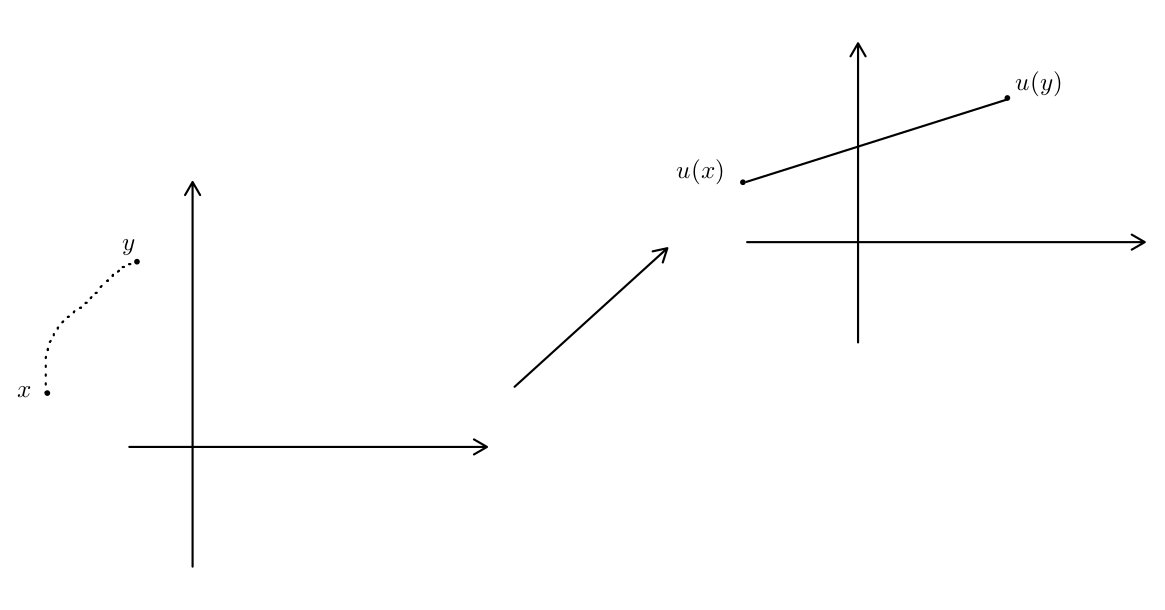
\includegraphics[scale=0.3]{figures/fig10.png}
  \caption{}
  \label{}
\end{figure}

%%%fig11%%%%

\begin{figure}[h!]
  \centering
  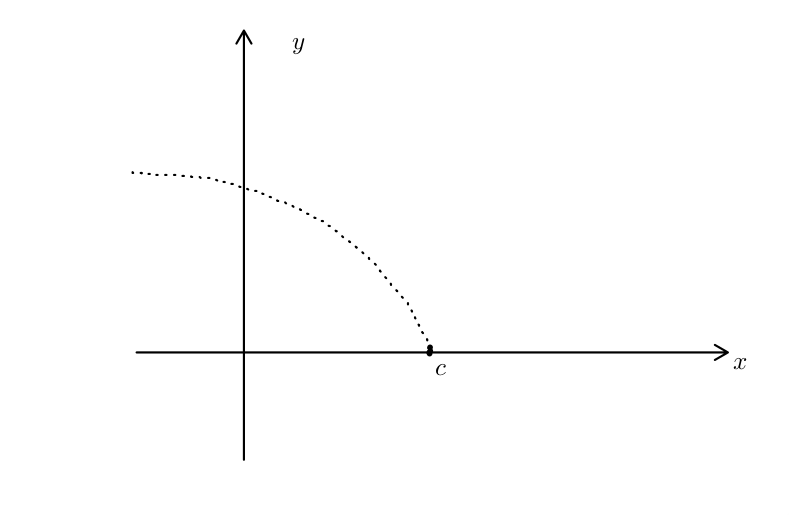
\includegraphics[scale=0.3]{figures/fig11.png}
  \caption{}
  \label{}
\end{figure}

\marginnote{14-11-2023}

\subsection{D\'erivation le long d'un champ de vecteurs}

Etant donné \(X\), on veut utiliser le difféomorphisme \(\Phi_t\) pour pousser ou retirer des champs de tenseurs sur \(U\). On a déjà vu que \(T \Phi_t(X(x))  = X(\Phi_t(x)), x \in U_t\),  ou bien en \'equivalence

\begin{equation}\label{cond_ch_tens}
  (\Phi_t)_{\sharp}(X \bigm|_{U_t}) = X \bigm|_{\Phi_t(U_t)},
\end{equation} c.\`a.d. le flot de $X$ laisse a champ de vecteur $X$ invariant. On peut interpr\'eter  ce fait par dire que le champ de vecteur $X$ est \lq \lq constant" le long de $X$. Une question est alors pos\'ee: quand est-ce qu'on peut dire qu'un champ de tenseur quelconque est constant le  long de $X$? (Par exemple, si le champ de tenseur en question est un autre champ de vecteur $Y$, et pas $X$ lui-m\^eme).

%fig12


\subsubsection{D\'erivation  d'un champ scalaire (fonction r\'eelle) le long d'un champ de vecteurs}

\begin{definition}

  Soit \(U \subset \mathbb{R}^n\) un ouvert.
  Etant donné un champ de vecteurs \(X : U \longrightarrow T U\) de régularité \(\mathcal{C}^1\) et l'application r\'eelle \(f : U \longrightarrow \mathbb{R}\) de régularité \(\mathcal{C}^1\). On définit

  \[X \cdot f(x) \stackrel{\text{déf}}{=} d_x f(X(x)) = D _{\mid X(x) \rangle} f.\]


Doc $X\cdot f(x) $ est en effet la d\'eriv\'ee directionnelle de $f$ \`a $x$, dans la direction de $X(x)$.    {\fontencoding{U}\fontfamily{futs}\selectfont\char 66\relax} Le point n'est pas l'opération de multiplication ici. $\lq \lq X\cdot"$ agit comme un op\'erateur diff\'erentielle.

  On a pour  \(X\) donn\'e en coordonnées  \(X =\displaystyle \sum_{i=1}^{n} X ^{i}\displaystyle \frac{\partial  }{\partial x ^{i}}\) et la fonction  \(f\),


  \begin{gather*}
    X \cdot f(x) = d_x f \left(\sum_{i=1}^{n} X ^{i}(x) \frac{\partial  }{\partial x ^{i}}(x) \right) = \sum_{i=1}^{n}X ^{i}(x)d_xf \left(\frac{\partial  }{\partial x ^{i}}(x) \right) = \sum_{i=1}^{n} X ^{i}(x) \frac{\partial f }{\partial x ^{i}}
  \end{gather*}

On revient en fait à la dérivée directionnelle de \(f\)  dans a direction de $X(x)$.
\end{definition}

Si \(X = \displaystyle \frac{\partial  }{\partial x ^{i}}\) (rappel : \(\displaystyle \frac{\partial  }{\partial x ^{i}}(x) = (x,e_i) \in T_x U\)).

On obtient

\[\frac{\partial  }{\partial x ^{i}} \cdot f = \frac{\partial f }{\partial x ^{i}}.\]

\begin{prop}
  Supposons que \(X\) est un champ de vecteurs \(\mathcal{C}^{\infty}\) sur \(U\) et \(f\) est une fonction \(\mathcal{C}^{\infty}\) sur \(U\). Si \(\Phi_t\) est le flot de \(X\), on a

  \[\forall x \in U, X \cdot f(x)  = \lim_{t \to 0} \frac{f(\Phi_t(x)) - f(x)}{t}.\]
\end{prop}


\begin{proof}


 Rappeler que   \(\gamma_x(t)\) est la courbe int\'egrale pour $X$, d\'efinie sur $I_x$, l'interval ouvert de taille positive, et $0\in I_x$. On a

\[
  \begin{aligned}
    \lim_{t \to 0} \frac{f(\Phi_t(x)) - f(x)}{t} & = \lim_{t \to 0} \frac{f \circ \gamma_x(t) -  f \circ \gamma_x(0)}{t} = (f \circ \gamma_x)'(0)\\ &  = Df(\gamma_x(0)) \gamma_x'(0) = Df(x) \mid X(x) \rangle = D _{\mid X(x) \rangle} f = X \cdot f(x),
  \end{aligned}
\] car \(\gamma'_x(0) = \mid X(\gamma_x(0))\rangle = \mid X(x) \rangle \). \end{proof}

\begin{remark}[Commentaires]

  \

  \begin{enumerate}
    \item   Pour tout \(x \in U,\, \Phi_t\) est défini pour \(t \in I_x\) l'intervalle maximal qui est de taille positive. Donc il existe \(\delta_x \bg 0\) tel que \(\Phi_t(x)\) est défini pour \(\left\lvert t \right\rvert \less \delta_x\). Donc

      \[ \frac{f(\Phi_t(x)) - f(x)}{t}\]

      est défini pour \(0 \less \left\lvert t \right\rvert \less \delta_x\).


\item
  La proposition est équivalente à
  \[
  X \cdot f(x) = \frac{d}{dt} \Big (f\circ \Phi_t(x)\Big) \bigm|_{t=0}.
  \]

    \item %fig13
Le pull-back d'un champ scalaire $f$ est d\'efini canoniquement par $(\Phi_t)^{*}f := f\circ \Phi_t$.  Donc
    \[X \cdot f(x) = \lim_{t\to 0} \frac{\Phi_t ^{*}f(x)-f(x)}{t} = \frac{d}{dt}(\Phi_t)^{*}f(x) \bigm|_{t=0}. \]

    \item
     Si \(Y\) est un autre champ de vecteur tel que \(X(x) = Y(x)\) pour \(x\) fixé, on obtient \(X \cdot f(x) = Y \cdot f(x)\).

  On a

  \begin{gather*}
    \frac{f(\Phi_t(x))-f(x)}{t} = \frac{f(\gamma_x(t)) -f(x)}{t} = \frac{f \circ \gamma_x(t)-f \circ \gamma_x(0)}{t},
  \end{gather*} Donc la valeur de  $X \cdot f(x)$ ne d\'epend qu'\`a la valeur de $X$ au point $X$ et des valeurs de $f$ dans un voisinage de $X$, m\^eme si la proposition connecte cette valeur au flot de $X$, qui lui par contre d\'epend des valeurs de $X$ dans un voisinage de $x$. Cette d\'ependance devient plus importante dans le cas de d\'erivation d'un champ de tenseur.
  \end{enumerate}
\end{remark}
 \subsubsection{Crochet de Lie \\
 (D\'erivation d'un champ de vecteur $Y$  le long du champ de vecteur $X$)}

\emph{On voudrait mesurer les variations d'un champ de vecteurs \(Y\) le long d'un autre champ de vecteurs $X$, utilisant le flot \(\Phi_t\)  de $X$.}

%fig14

Fixons \(x \in U\). On a \(Y(x) \in T_x U\). Comme $Y$ est un champ de tenseur contra-variant, on doit utiliser les push-forward au lieu des pull-backs pour pouvoir comparer les valeurs de $Y$ le long d'un autre champ de vecteur sur un point $x$. Donc, pour revenir \`a $x$ d'un point $\Phi_t(x)$, il faudra utiliser le push-froward par le diff\'eomorphisme  $\Phi_{-t}$.

%fig15

On remarque que \(\Phi _{-t} : \Phi_t(U_t) \longrightarrow U\) est un \textbf{difféomorphisme}, et donc, comme \(x \in U_t\) pour \(\left\lvert t \right\rvert \less \delta_x, \Phi_t(x) \in \Phi_t(U_t)\),  on obtient que \((\Phi _{-t})_{\sharp}Y(x)\) est défini.

On rappelle que \((\Phi _{-t})_{\sharp}Y(x) = T \Phi _{-t}(Y (\Phi_t(x)))\), avec
\[T{\Phi _{-t}}\bigm|_{T _{\Phi _{t}(x) }U} : T _{\Phi_t(x)} U \longrightarrow T_x U.\]

Donc on peut définir, pour \(0 \less \left\lvert \delta_x \right\rvert\),

\[\frac{(\Phi _{-t})_{\sharp}Y(x) - Y(x)}{t} \in T_xU.\]

\emph{Question : Est-ce que cette limite existe et quelle est sa valeur ?}

Si la limite existe pour tout \(x \in U\), on observe que

\[\lim_{t \to 0} \frac{(\Phi _{-t})_{\sharp}Y(x)-Y(x)}{t} \in T_x U.\]

Donc on obtient un champ de vecteurs (c.\`a. d. un \'el\'ement de $T_xU$ pour chaque $x \in u$) par cette limite. Maintenant on veut \textbf{identifier ce champ de vecteurs}.

\begin{definition}\label{crochet-de-lie}
  Soient \(X,Y\) deux champs de vecteurs sur \(U\) de régularité \(\mathcal{C}^{\infty}\). Il existe un champ de vecteurs unique nommé \textbf{le crochet de Lie de \(X\) et \(Y\)} et dénoté par \([X,Y]\) tel que

  \[\forall f \in \mathcal{C}^{\infty}(U), \quad [X,Y] \cdot f = X \cdot (Y \cdot f) - Y \cdot (X \cdot f).\]
\end{definition}

\begin{remark}
Le fait qu'un champ de vecteur unique avec une telle propri\'et\'e  existe est un fait non-\'evident. On ne va pas le d\'emontrer ici.
\end{remark}
\begin{remark}
Par la d\'efinition,  on obtient directement que pour tous champs de vecteurs $X$ et $Y$ on a
\[ [X, X]  = 0 \,\, \mbox{et} \,\, [Y, X] = - [X,Y]. \]
\end{remark}

\begin{thm}\label{crochet-lie}
  Soient \(X,Y\) des champs de vecteurs \(\mathcal{C}^{\infty}\) et \(\Phi_t\) flot de \(X\). Alors pour tout \(x \in U\),

  \[[X,Y](x) = \lim_{t \to 0} \frac{(\Phi _{-t})_{\sharp}Y(x) - Y(x)}{t}=  \frac{d}{dt} (\Phi_{-t})_{\sharp}Y(x) \bigm|_{t=0}.\]
\end{thm}

\begin{corollary}
  Si \(\Psi_t\) est le flot de \(Y\), alors

  \[[Y,X](x) = \lim_{t \to 0} \frac{(\Psi _{-t})_{\sharp}X(x)-X(x)}{t},\]

  mais \([X,Y] = - [Y,X]\). Donc

  \[[X,Y] = -  \lim_{t \to 0} \frac{(\Psi _{-t})_{\sharp}X(x)-X(x)}{t}.\]
\end{corollary}

\begin{prop}\label{crochet-zero}
Pour tout $x\in U$, et pour \(t,s\) assez petit on a \(\Phi_t \circ \Psi_s (x)= \Psi_s \circ \Phi_t (x)\) si et seulement si \([X,Y] \equiv 0\). Dans ce cas,
\[
\forall x\in U \quad  \Phi_t \circ \Psi_s (x)= \Psi_s \circ \Phi_t (x)
\] pour tout $t,s$ pour lesquels les deux expressions sont d\'efinies.

(En \'equivalence, si et seulement si
\[
\Psi_{-s} \circ \Phi_{-t} \circ \Psi_s \circ \Phi_t (x) = x
\] pour tout $t,s$ pour lesquels l'expression de gauche est d\'efinie.)
\end{prop}
\begin{remark}
Pour tout \(x \in U, \exists \delta_x'\) tel que \(\forall  |t|,|s|  \less \delta_x'\),
\(\Psi_{-s} \circ \Phi _{-t} \circ \Psi_s \circ \Phi_t(x)\) est d\'efinie (pourquoi?).
\end{remark}
%fig16
\begin{remark}
Si \([X,Y] \neq 0\), alors il existe \(x \in U\) tel que les deux points
\[
x \quad \mbox{et} \quad \Psi_{-s} \circ \Phi_{-t} \circ \Psi_s \circ \Phi_t (x)
\] ne se rejoignent pas (cf figure).
\end{remark}

%fig17



\begin{proof}[Démonstration de la proposition \ref{crochet-zero}]
  Rappel : si \(h : U \longrightarrow V\) est un difféomorphisme et \(Y = h _{\sharp}X\), avec \(X : U \longrightarrow T U\) et \(Y : V \longrightarrow T V\), champs de vecteurs, alors \(\Psi_t = h \circ \Phi_t \circ h ^{-1}\).

 Supposons que \(\Phi_t \circ \Psi_s = \Psi_s \circ \Phi_t\) pour $t,s$ assez petit.  Cela implique que pour un $\delta_x$ assez petit, \[\Psi_s = \Phi_t \circ \Psi_{s} \circ (\Phi_t)^{-1}, \forall \left\lvert t \right\rvert, |s| \less \delta_x.\]  On fixe $t$ et on applique l'exercice \ref{flot-push} à \(h = \Phi_t\) (avec le param\`etre $s$ au lieu de $t$), et on obtient en conclusion que \[Y = h_\sharp Y = (\Phi_t)_{\sharp}Y,\]  qui veut dire
 \[
\forall x\in U \quad Y(x) = (\Phi_t)_\sharp Y (x) =  T\Phi_{t} (Y(\Phi_{-t}(x)).
\]
Comme l'argument est ind\'ependant  de $t$, ceci est vrai pour \( \forall t\,\, \left\lvert t \right\rvert \less \delta_x\). Donc, comme \(\left\lvert t \right\rvert \less \delta_x \iff \left\lvert -t \right\rvert \less \delta_x\), on obtient ainsi que \(\forall t, \left\lvert t \right\rvert \less \delta_x\), on a
  \(Y = (\Phi _{-t})_{\sharp}Y\) et donc

  \begin{gather*}
    [X,Y] = \lim_{t \to 0} \frac{(\Phi _{-t})_{\sharp}Y(x)-Y(x)}{t} = \lim_{t \to 0} \frac{Y(x)-Y(x)}{t} =0.
  \end{gather*}

  Réciproquement, on suppose que \([X,Y] \equiv 0\). Cela implique, par le th\'eor\`eme \ref{crochet-lie} que \(\forall x \in U\),

  \[\frac{d}{dt} (\Phi_{-t})_{\sharp}Y(x)\bigm|_{t=0} =  \lim_{t \to 0} \frac{(\Phi_{-t})_{\sharp}Y(x)-Y(x)}{t} =0. \]
On calcule maintenant, pour $Z(t):=  (\Phi_{-t})_{\sharp}Y(x) \in T_xU$, et \(\forall t\,\, \forall h\) t.q. \(-h \in I_{\Phi_t(x)}\)
\[
\begin{aligned}
 Z'(h)= \frac{d}{dt} (\Phi_{-t})_{\sharp}Y(x)\bigm|_{t=h}
& =  \lim_{t \to 0} \frac{(\Phi_{-(t+h)})_{\sharp}Y(x)-(\Phi_{-h})_{\sharp}Y(x)}{t}
\\ &   =  \lim_{t \to 0} \frac{(\Phi_{-h} \circ \Phi_{-t})_{\sharp}Y(x)-(\Phi_{-h})_{\sharp}Y(x)} {t}
\\ &  =  \lim_{t \to 0} \frac{(\Phi_{-h})_\sharp (\Phi_{-t})_{\sharp}Y(x)-(\Phi_{-h})_{\sharp}Y(x)}{t}
\\ &  =  (\Phi_{-h})_\sharp  \lim_{t \to 0} \frac{(\Phi_{-t})_{\sharp}Y(x)- Y(x)}{t} = (\Phi_{-h})_{\sharp} 0 =0.
 \end{aligned}
\]

On en d\'eduit que $Z$ est constant, c.\`a.d. pour tout $t$ t.q. $Z(t)$ est d\'efini, on a $Z(t) = Z(0)$. Donc
$$
\forall x\in U\,\, \forall t\in I_x \quad  (\Phi_{-t})_{\sharp}Y(x) = (\Phi_{0})_{\sharp}Y(x) = Y(x)
$$ ou bien, rempa\c cant $-t$ par $t$
$$
(\Phi_{t})_{\sharp}Y =Y.
$$ Fixant $t$ et appliquant la proposition \ref{flot-push-diff} \`a $h:= \Phi_t$, on obtient
$$
\Psi_s = \Phi_t \circ \Phi_s \circ \Phi^{-1}_{t}
$$ pour tout $s$ pour lequel les deux expressions sont d\'efinies.  Composant les deux c\^ot\'es avec $\Phi_t$, on obtient
\[
\Psi_s  \circ \Phi_t = \Phi_t \circ \Phi_s,
\] comme r\'equis.
\end{proof}

\marginnote{15-11-2023}

Pour la d\'emonstration du th\'eor\`eme \ref{crochet-lie}, on d\'emontre d'abord un lemme auxiliaire.

\begin{lemma}\label{rhox}
  Etant donné \(f \in \mathcal{C}^{\infty}(U) \text{ et } X : U \longrightarrow TU\) champ de vecteurs avec le flot \(\Phi\),  pour tout \(x \in U\), il existe $\delta_x>0$, et une application continue \(\rho_x : ] -\delta_x  , \delta_x[ \longrightarrow \mathbb{R}\) avec \(\rho_x(0) = X \cdot f(x)\) et \[f(\Phi_t(x)) = f(x)+t \rho_x(t).\] En plus, si $b_t(x) := \rho_x(t)$, alors $b_t$, pour chaque $t$, est de classe $\mathcal{C}^\infty$, et on a pour tout $\vec v \in T_x U$
\[
  \lim_{t\to 0} db_t (\vec v)  = db_0 (\vec v) = d (X\cdot f) (\vec v).
  \]  \end{lemma}

\begin{proof}
  On met \(u(t) = f(\Phi_t(x))\) et donc

  \[u'(t)\bigm|_{t=0} = \lim_{t \to 0} \frac{f(\Phi_t(x))-\stackrel{f(\Phi_0(x))}{f(x)}}{t} = X \cdot f(x). \]

  Par conséquent

  \[\lim_{t \to 0} \frac{u(t)-u(0)}{t} = X \cdot f(x).\]

On d\'efinit

  \[\rho_x(t) := \begin{cases}
    \displaystyle \frac{u(t)-u(0)}{t} & \text{ si } t \neq 0,\, t \text{ assez petit} \\
    X \cdot f(X) &  \text{ si } t=0.
  \end{cases}\] qui est naturellement continue sur un interval \([-\delta_x, \delta_x[\) pour un choix assez petit de $\delta_x$.  Alors

  \[\rho_x(t) = \frac{u(t)-u(0)}{t} \implies u(t)=u(0)+t \rho_x(t) = f(x)+ t \rho_x(t),\] et \(\rho_x(0)= X \cdot f(x).\)

  Maintenant, on observe que pour tout $\vec v \in T_xU$
   \[
   \begin{aligned}
 d \Big ( \lim_{t \to 0} \frac{f\circ \Phi_t - f}{t}   \Big )  (\vec v)
 & = D_{|\vec v\rangle}\Big ( \lim_{t \to 0} \frac{f\circ \Phi_t - f}{t}   \Big )  (x)
 \\ &  = \lim_{h\to 0} \frac 1h \Big [ \lim_{t \to 0}  \Big ( \frac{f\circ \Phi_t - f}{t}   \Big )  (x+h|\vec v\rangle ) -  \Big (\lim_{t \to 0} \frac{f\circ \Phi_t - f}{t}   \Big )(x) \Big ]
  \\ &  = \lim_{t\to 0}      \lim_{h \to 0} \frac 1h \Big [\Big ( \frac{f\circ \Phi_t - f}{t}   \Big )  (x+h|\vec v\rangle ) -  \Big (\frac{f\circ \Phi_t - f}{t}  \Big ) \Big ] (x)  \\ &
  = \lim_{t\to 0} d\Big (\frac{f\circ \Phi_t - f}{t}\Big )   (\vec v),
      \end{aligned}
 \] (pourquoi?) et donc
  \[
  d(X\cdot f) (\vec v) = d\Big ( \lim_{t \to 0} \frac{u(t)-u(0)}{t} \Big )  (\vec v)= d \Big ( \lim_{t \to 0} \frac{f\circ \Phi_t - f}{t}   \Big ) (\vec v) = \lim_{t\to 0} db_t (\vec v)
  \] pour $b_t(x) := \rho_x(t)$.
\end{proof}

\begin{proof}[Démonstration du théorème \ref{crochet-lie}]
  Pour d\'emontrer le théorème, il faut montrer que \(\forall f \in \mathcal{C}^{\infty}(U), \forall x \in U\),

  \[d_x f \left(\lim_{t \to 0} \frac{(\Phi _{-t})_{\sharp} Y(x)- Y(x)}{t} \right) \stackrel{?}{=} X \cdot(Y \cdot f)- Y \cdot(X \cdot f).\]

  On a

  \begin{gather}\label{expression-compliquee}
 \begin{aligned}
    d_x f \left(\lim_{t \to 0} \frac{(\Phi _{-t})_{\sharp} Y(x) - Y(x)}{t} \right) &
     = \lim_{t \to 0} d_x f \left(\frac{(\Phi _{-t})_{\sharp}Y(x)-Y(x)}{t}\right)
     \\ & = \lim_{t \to 0} \frac{d_x f((\Phi _{-t})_{\sharp} Y(x))- d_xf (Y(x))}{t} \\ &
    = \lim_{t \to 0} \frac{d_x f((\Phi _{-t})_{\sharp} Y(x)) - Y \cdot f(x)}{t}
    \\ &  = \lim_{t \to 0} \frac{d_x f(T\Phi _{-t}(Y(\Phi_t(x))))- Y \cdot f(x)}{t}.
     \end{aligned}
 \end{gather}


Rappeler que par l'exemple \ref{dfoT},  pour \(g : U \longrightarrow V, f : V \longrightarrow \mathbb{R}, d (f \circ g) = df \circ Tg\). Appliquant cela \`a $g:= \Phi_{-t}$, on obtient
\[
d_x f(\underbrace{T\Phi _{-t}(Y(\Phi_t(x)))}_{\in T_x U}) = df \circ T\Phi_{-t} (Y(\Phi_t(x))) = d(f\circ \Phi_{-t}) (Y(\Phi_t(x))) = d(f - tb_{-t})  (Y(\Phi_t(x)))
\] Alors, par \eqref{expression-compliquee}
    \begin{gather*}
     \begin{aligned}
  d_x f \left(\lim_{t \to 0} \frac{(\Phi _{-t})_{\sharp} Y(x) - Y(x)}{t} \right)   &  = \lim_{t \to 0} \frac{d (f - t b_{-t}) (Y(\Phi_t(x)))- Y \cdot f(x)}{t} \\ &  =  \lim_{t \to 0} \frac{d _{\Phi_t(x)} f(Y (\Phi_t(x))) - Y \cdot f(x) - td b_{-t}(Y (\Phi _{-t}(x)))}{t}
   \\  &   = \lim_{t \to 0} \frac{Y \cdot f(\Phi_t(x))- Y \cdot f(x)}{t}- \lim_{t \to 0}  d b_{-t}(Y (\Phi _{-t}(x)))
     \\  &    =  X \cdot(Y \cdot f)(x) -  d (X\cdot f) (Y(x)) \\ & = X \cdot(Y \cdot f)(x) - Y \cdot(X \cdot f)(x),
    \end{aligned}
  \end{gather*} comme $Y(\Phi_{-t}(x))$ converge vers $Y(x)$ dans $TU$, $db_t : TU \to \R$ est continue, et   par le lemme ci-dessus
\[
  \lim_{t \to 0}db_t (Y(x))  =   d(X \cdot f) (Y(x)) = Y\cdot (X \cdot f) (x).
  \] \end{proof}

\subsubsection{Calcul de \([X,Y]\) dans les coordonnées} Soit \(X = \displaystyle\sum X ^{i}\displaystyle\frac{\partial  }{\partial x ^{i}}, Y =  \displaystyle\sum Y ^{i}\displaystyle\frac{\partial  }{\partial x ^{j}}\)


On a \(X \cdot f = \displaystyle \sum_{i}^{} X ^{i} \displaystyle \frac{\partial f }{\partial x ^{i}}, Y \cdot f = \displaystyle \sum_{j}^{} Y ^{j} \displaystyle \frac{\partial f }{\partial x ^{j}}\).

Alors

\begin{gather*}
  X \cdot (Y \cdot f) = \sum_{i} X ^{i} \left(\frac{\partial (Y \cdot f) }{\partial x ^{i}} \right), Y \cdot(X \cdot f) = \sum_{j} Y ^{j} \left(\frac{\partial (X \cdot f) }{\partial x ^{j}} \right),
\end{gather*}

ce qui donne

\begin{gather*}
  [X \cdot Y] \cdot f = X \cdot (Y \cdot f) - Y \cdot (X \cdot f) \\
  = \sum_{i}^{} X ^{i}\left(\frac{\partial  }{\partial x ^{i}} \left(\sum_{j} Y ^{j}\frac{\partial f }{\partial x ^{j}}  \right)\right) - \sum_{j} Y^{j}\left(\frac{\partial  }{\partial x ^{j}} \left(\sum_{i} X^{i}\frac{\partial f }{\partial x^{i}}  \right)\right) \\
  = \sum_{i}\sum_{j} X ^{i} \frac{\partial Y ^{j} }{\partial x ^{i}} \frac{\partial f }{\partial x ^{j}} + \sum_{i}\sum_{j} X ^{i} Y ^{j} \frac{\partial ^2 f }{\partial x ^{i}\partial x ^{j}} - \sum_{j}\sum_{i} Y^{j} \frac{\partial X^{i} }{\partial x ^{j}} \frac{\partial f }{\partial x^{i}} - \sum\sum Y^{j} X^{i} \frac{\partial ^2 f }{\partial x^{j} \partial x^{i}} \\
  = \sum_{i,j} X ^{i} \frac{\partial Y ^{j} }{\partial x ^{i}} \frac{\partial f }{\partial x ^{j}} - Y ^{j} \frac{\partial X ^{i} }{\partial x ^{j}} \frac{\partial f }{\partial x ^{i}}  = \sum_{i} \sum_{j} \left(X ^{j}\frac{\partial Y ^{i} }{\partial x ^{j}} - Y ^{j} \frac{\partial X ^{i} }{\partial x ^{j}} \right)  \frac{\partial f }{\partial x^{i}}.
\end{gather*}

Si \([X,Y] = \displaystyle \sum_{i} [X,Y]^{i}\displaystyle\frac{\partial  }{\partial x ^{i}}\), alors \([X,Y]\cdot f = \displaystyle \sum_{i}[X,Y]^{i}\displaystyle\frac{\partial f }{\partial x ^{i}}\). Donc

\[[X,Y]^{i} = \sum_{j} \left(X ^{j} \frac{\partial Y ^{i} }{\partial x ^{j}} - Y ^{j}\frac{\partial X ^{i} }{\partial x ^{j}}\right).\]

Donc si
$$
X(x) = (x, \vec F(x)), Y(x) = (x, \vec G(x))
$$ pour $\vec F, \vec G : U \to \R^n$, on obtient
$$
[X,Y](x)=  (x, D\vec G(x) {\vec F(x)} - D \vec F (x) {\vec G(x)}) =
(x, D_{\vec F(x)}\vec G(x) - D_{\vec G(x)} \vec F (x)).
$$  On peut \'ecrire plus consis\'ement
$$
\Big | [X,Y] \Big \rangle  =   D_{\vec F}\vec G - D_{\vec G} \vec F = D_{|X\rangle} |Y\rangle- D_{|Y\rangle} |X\rangle,
$$ o\`u pour tout champ de vecteur $X(x)= (x, |X\rangle(x)) \in T_xU$, $ |X\rangle : U \to \R^n$.
\begin{exemple}
  Si \(X = \displaystyle \frac{\partial  }{\partial x ^{i}}, Y = \displaystyle \frac{\partial  }{\partial x ^{j}}\), on a \(\displaystyle \left[\frac{\partial  }{\partial x ^{i}}, \frac{\partial  }{\partial x ^{j}}  \right] = 0\).
\end{exemple}

\begin{exemple}\label{cro-non0}
  Posons, sur \(\mathbb{R} \setminus \{ 0 \} = U\),

  \begin{gather*}
    X(x,y) = \frac{x}{\sqrt{x ^2 + y ^2}}\frac{\partial  }{\partial x} + \frac{y}{\sqrt{x ^2 + y ^2}} \frac{\partial  }{\partial y} \\
    Y(x,y) = - \frac{y}{\sqrt{x ^2 + y ^2}}\frac{\partial  }{\partial x} + \frac{x}{\sqrt{x ^2 + y ^2}} \frac{\partial  }{\partial y}.
  \end{gather*}

  Le point d'arrivée après l'application de \(\Psi _{-s} \circ \Phi _{-t} \circ \Psi _{s} \circ \Phi _{t}\) est (dans les coordonnées polaires) \(\left(r, \theta + \displaystyle \frac{s}{r+t}- \displaystyle \frac{s}{r}\right) \neq (r,\theta)\).

  Or d'après la proposition \([X,Y] = 0 \iff \Psi_s \circ \Phi_t = \Phi_t \circ \Psi_s\). On ne peut donc pas avoir \([X,Y]=0\). On a par ailleurs :

  \begin{gather*}
    |X \rangle  (x,y) = \overrightarrow{F}(x,y) = \begin{bmatrix}
      \frac{x}{\sqrt{x ^2 + y ^2}} \\
      \frac{y}{\sqrt{x ^2 + y ^2}}
  \end{bmatrix},     |Y \rangle  (x,y)=  \overrightarrow{G}(x,y) = \begin{bmatrix}
    - \frac{y}{\sqrt{x ^2 + y ^2}}\\
    \frac{x}{\sqrt{x ^2 + y ^2}}
\end{bmatrix}.
  \end{gather*}

  \begin{exo}\label{cro-exo1}
  Calculer $[X, Y]$.
  \end{exo}
\end{exemple}


\subsubsection{Quelques propriétés du Crochet de Lie}


\begin{prop}\label{gamma'}
 Soit \(\Gamma(t) = \Psi _{-t} \circ \Phi _{-t}\circ \Psi_t \circ \Phi_t(x) \in U\). Alors on a \(\Gamma(0) = x\), \(\Gamma'(0) = 0\), \(\Gamma''(0) = 2 [X,Y](x)\). \textcolor{red}{check!}
\end{prop}
  %%diagramme
\begin{exemple}
En retour \`a l'exemple \ref{cro-non0}, on obtient dans les coordon\'ees polaires le commutateur des deux flots est donn\'e par
  \((r,\theta)\longmapsto \left(r,\theta+ \frac{s}{r+t}-\frac{t}{r}\right)\).  Alors on  obtient \(\Gamma(t)(r,\theta) = \left(r,\theta+ \frac{s}{r+t}-\frac{t}{r}\right)\) en coordonnées polaires. En coordonnées euclid\'eenne, on a alors

  \begin{gather*}
    \Gamma(t) = \left(r \cos \left(\theta+\frac{t}{r + \theta} - \frac{t}{r}\right), r \sin \left(\theta+ \frac{t}{r+\theta}- \frac{t}{r}\right)\right) = (r \cos(\theta(t)), r \sin(\theta(t))).
  \end{gather*}
    \begin{exo}\label{cro-exo2}
  Calculer $\Gamma''(0)$ et utiliser la proposition \ref{gamma'} pour obtenir  $[X, Y]$. Comparer avec l'exercice \ref{cro-exo1}.
  \end{exo}
\end{exemple}



\begin{prop}

  \

  \begin{enumerate}
    \item Pour tous \(X,Y\) champs de vecteurs, \([X,Y] = -[Y,X]\).
    \item Pour tout \(X\) champ de vecteurs, \([X,X] = 0\).
    \item Pour tout \(c \in \mathbb{R}, [cX,Y] = c[X,Y]\) et \([X,cY] = c[X,Y]\) et

    \begin{gather*}
      \forall X, \widetilde{X}, Y, \widetilde{Y}, [X+ \widetilde{X}, Y] = [X,Y]+ [\widetilde{X}, Y], [X,Y + \widetilde{Y}] = [X,Y] + [X,\widetilde{Y}].
    \end{gather*}

    \item Pour tous \(X,Y,Z \in \mathcal{C}^{\infty}\),

    \[[[X,Y], Z] + [[Y,Z],X]+ [[Z,X],Y] \equiv 0.\]

    {\fontencoding{U}\fontfamily{futs}\selectfont\char 66\relax} \([X,Y]\) n'est pas linéaire par multiplication par une fonction scalaire non constante.

    \item \label{crochet-lie-fct} Pour \(f \in \mathcal{C}^{\infty}(U), f X(x) \stackrel{\text{déf}}{=}f(x)X(x)\), on a

    \[\begin{cases}
      [fX,Y] = f [X,Y]-(Y \cdot f)X \\
      [X,f Y] = f[X,Y] + (X \cdot f)Y.
    \end{cases}\]
  \end{enumerate}
\end{prop}

\begin{proof}
  On démontre le point \ref{crochet-lie-fct}. Pour d\'eterminer $[fX, Y]$, selon la d\'efinition \ref{crochet-de-lie}, il faut trouver son action sur un champ scalaire $f=g$. On a

  \begin{gather*}
    [fX,Y]\cdot g = (fX) \cdot (Y \cdot g)  - Y \cdot(f X \cdot g) = (f X) \cdot (Y \cdot g) - Y \cdot (f (X \cdot g)) \\
    = f(X \cdot(Y \cdot g)) - d(f(X \cdot g))(Y)
    = f(X \cdot(Y \cdot g)) - (X \cdot g)d f(Y) - f d (X \cdot g)(Y)  \\ = f(X \cdot(Y \cdot g)) - (X \cdot g)(Y \cdot f) - f Y \cdot (X \cdot g)
    = f((X \cdot (Y \cdot g)) - Y \cdot (X \cdot g))- (Y \cdot f)(X \cdot g)\\  = (f [X,Y] - (Y \cdot f)X) \cdot g.
  \end{gather*}
\end{proof}

\subsubsection{D\'eriv\'ee de Lie d'un champ tensoriel}

Soit \(X\) un champ de tenseur \(\mathcal{C}^{\infty}\) avec le flot \(\Phi\). Soit \(\alpha : U \longrightarrow T ^{k} U\) un champ de tenseurs covariant.

\begin{definition}
  On définit la dérivée de Lie de \(\alpha\) le long de \(X\) par

  \[\forall x \in U \quad \mathcal{L}_X \alpha(x) \stackrel{\text{déf}}{:=} \lim_{t \to 0} \frac{(\Phi_t)^{*} \alpha(x)-\alpha(x)}{t} \in T_x ^{k} U = \Omega ^{k}(T_x U).\]
\end{definition}

\begin{remark}[Rappel]
  On a

  \[(\Phi_t)^{*}\alpha(x)(\overrightarrow{v_1}, \dots, \overrightarrow{v_k}) = \alpha(\Phi_t(x))(T \Phi_t(\overrightarrow{v_1}), \dots, T \Phi_t(\overrightarrow{v_k})).\]
\end{remark}

Donc \(\mathcal{L}_X \alpha : U \longrightarrow T ^{k} U\) est aussi un champ de tenseurs. Si \(X \in \mathcal{C}^{\infty}, \alpha\) est \(\mathcal{C}^{\infty}\), alors \(\mathcal{L}_X \alpha\) est aussi \(\mathcal{C}^{\infty}\).

\begin{definition}
  Si \(\beta : U \longrightarrow T_l U\) est un champ de tenseurs contravariant, on définit la dérivée de Lie de \(\beta\) le long de \(X\) par

  \[\mathcal{L}_X \beta \stackrel{\text{déf}}{:=} \lim_{t \to 0}\frac{(\Phi _{-t})_{\sharp} \beta - \beta}{t}.\]
\end{definition}

\(\mathcal{L}_X \beta : U \longrightarrow T_l U\) est aussi un champ de tenseur contravariant, de même ordre, et si $X$ est \(\mathcal {C}^\infty\), il est de la même régularité de \(\beta\).

Si l'on interprète une fonction scalaire $f:U \to \R$, comme un champ de l'ordre 0 (\(\forall x \in U, f(x) \in \Lambda ^{0}(T_x U) \simeq \mathbb{R}\)). On peut alors écrire

\[X \cdot f = \mathcal{L}_X f = df(X).\]

Si \(Y\) est un champ de vecteur sur \(U\), on obtient, comme \(Y : U \longrightarrow T_1 U = TU\) un champ de tenseurs contravariants de l'ordre 1, \([X,Y] = \mathcal{L}_X Y\). Notez que \[\mathcal{L}_X \beta = - \lim_{t \to 0} \frac{(\Phi_t)_{\sharp} \beta - \beta}{t}.\]

\begin{exemple}
  On a, pour \(X,Y\) champs de vecteur avec \(\mathcal{L}_X Y =0\), \([X,Y] = 0\) si et seulement si \(\Phi_t \circ \Psi_s = \Psi_s \circ \Phi_t\). On pose \( |X(x,y)\rangle  = \left(\frac{x}{r}, \frac{y}{r}\right), |Y(x,y)\rangle  = (-y,x), U = \mathbb{R}^2 \setminus \{ 0 \}\).

  Donc pour cet exemple, on a

  \begin{gather*}
    X = \frac{x}{r}\frac{\partial  }{\partial x} + \frac{y}{r}\frac{\partial  }{\partial y}\\
    X = -y \frac{\partial  }{\partial y}+ x \frac{\partial  }{\partial y}.
  \end{gather*}

  Alors on a \(\mathcal{L}_X Y = [X,Y]=0\) et \(\mathcal{L}_Y X \equiv [Y,X] \equiv -[X,Y]\equiv 0\) (exercice).

Donc \(X\) est \lq \lq constant\rq \rq \,le long du flot de \(Y\) (c.\`a. d. sous l'action du flot de $Y$), et \(Y\) est \lq \lq constant\rq \rq \,le long du flot de \(X\), on a la situation décrites dans la figure \ref{flotXY}.

  Voir illustrations \ref{exemple_gamma_psi_phi} et \ref{flotXY}.
\end{exemple}

\begin{remark}
En principe, si ${\bf x} \neq {\bf y}$ pour ${\bf x},{\bf y} \in U$, on ne peut pas comparer $X({\bf x})$ et $X({\bf y})$ comme ils appartiennent aux espaces tangents  diff\'erents. Donc la notion d'un champ de vecteurs constant devient plus compliqu\'e et d\'epend de type de d\'efinition qu'on en donne.
\end{remark}

\begin{figure}[h!]
  \centering
  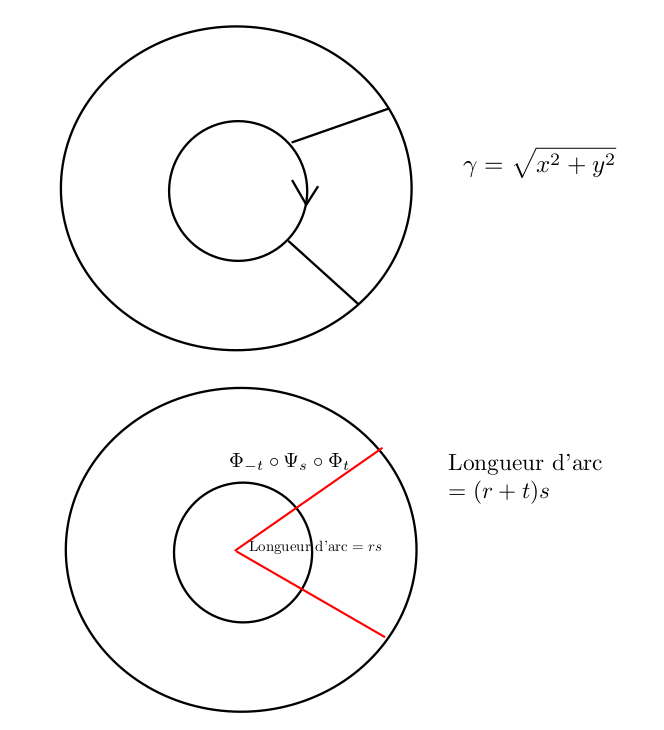
\includegraphics[scale=0.3]{figures/exemple_gamma_psi_phi.png}
  \caption{Illustration de l'exemple. \textcolor{red}{l'image \`a s'am\'eliorer} Dans ce cas, on a bien \(\Psi _{-t} \circ \Phi _{-t}\circ \Psi_s \circ \Phi_t = \operatorname{id}\).}
  \label{exemple_gamma_psi_phi}
\end{figure}

\begin{figure}[H]
  \centering
  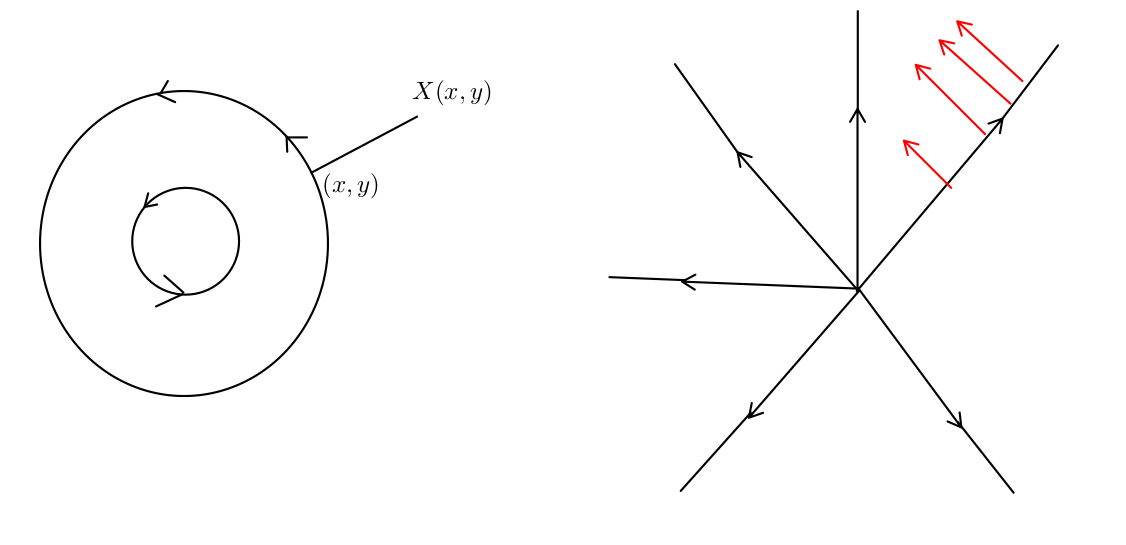
\includegraphics[scale=0.3]{figures/flotXY.png}
  \caption{Le flot de \(X\) et de \(Y\) tels qu'ils étaient définis dans l'exemple. \textcolor{red}{l'image \`a s'am\'eliorer}}
  \label{flotXY}
\end{figure}

\begin{thm}
  Si \(\alpha\) est un champ de tenseurs soit covariant d'ordre \(k\) soit contravariant d'ordre \(l\), si \(X\) est un champ de vecteurs sur \(U\) de régularité \(\mathcal{C}^{\infty}\), alors

  \[\mathcal{L}_X \alpha = 0 \iff \begin{cases}
    \alpha \text{ contravariant, } \alpha = (\Phi_t)_X ^{*} \quad  \forall t  \text{ quand } \Phi_t \text{ est défini}, \\
    \alpha \text{ contravariant, } \alpha = (\Phi_t)_{\sharp}\alpha, \quad \forall t \text{ quand } \Phi _{t} \text{ est défini. }
  \end{cases}\]
\end{thm}

\begin{proof}
  On fait la preuve dans le cas où \(\alpha\) est covariant. Pour le cas où \(\alpha\) est contravariant, la démonstration est similaire.

  Si \(t\) est assez petit, on a \((\Phi_t)^{*}\alpha = \alpha\), alors

  \[\mathcal{L}_X \alpha = \lim_{t \to 0}\frac{(\Phi_t)^{*} \alpha - \alpha}{t} = \lim_{t \to 0} \frac{0}{t}=0.\]

  Maintenant supposons que \(\mathcal{L}_X \alpha = 0\). On a alors, pour tout \(x \in U\),

  \[\lim_{t \to 0}\frac{(\Phi_t)^{*} \alpha(x)- \alpha(x)}{t}=0.\]

  On fixe \(h\) et on calcule pour \(\Phi _{t+h} = \Phi_t \circ \Phi_h\).

  \begin{gather*}
    I = \lim_{t \to 0}\frac{(\Phi _{t+h})^{*}\alpha(x)-\Phi_h ^{*}\alpha(x)}{x} = \lim_{t \to 0} \frac{(\Phi_t \circ \Phi_h)^{*} \alpha(x)- \Phi_h ^{*}\alpha(x)}{t} \\
    = \lim_{t \to 0} \frac{(\Phi_h ^{*}(\Phi_t ^{*} \alpha))(x) - (\Phi_h ^{*} \alpha)(x)}{t}   = \lim_{t \to 0}\left[(\Phi_h)^{*} \left(\frac{(\Phi_t ^{*} \alpha) - \alpha}{t}\right)\right](x)\\
    = \left[\Phi_h ^{*} \left(\lim_{t \to 0}\frac{(\Phi_t ^{*} \alpha)-\alpha}{t} \right)\right](x).
  \end{gather*}

  Si \(h\) est fixé, on note \(y = \Phi_h(x)\) et on obtient

  \[\lim_{t \to 0}\frac{\Phi_t ^{*}\alpha(y) - \alpha(y)}{t}=0,\]

  donc

  \[\lim_{t \to 0} \frac{\Phi_t ^{*} \alpha - \alpha}{t}(\Phi_h (x))=0.\]

  Donc \(\Phi_h ^{*}\left(\displaystyle  \lim_{t \to 0} \frac{\Phi_t ^{*}\alpha- \alpha}{t} \right)(x)= 0\) (pourquoi?), ce qui implique \(I=0\).


Mais d'un autre point de vue,

\[I = \frac{d}{dt}[(\Phi_t ^{*}\alpha)(x)]\bigm|_{t=h},\] où \(\Phi^*_t \alpha(x) \in T_x ^{k} U\) pour tout \(t\) assez petit. On définit \(t \stackrel{\Gamma}{\longmapsto}T_x ^{k}U, \Gamma(t):=\Phi_t ^{*} \alpha(x)\) et on a remarqué que \(I = \Gamma'(h)\). On a vu que \(I=0\), et \(h\) étant quelconque, on a par conséquent pour tout \(h, \Gamma'(h)=0\), donc \(\Gamma \equiv \text{constante}.\)

On conclut que \(\Phi_t^{*}\alpha(x) = \Phi_0^{*}\alpha(x) = \alpha(x)\) pour tout \(t\) pour lequel \(\Phi_t^{*}\alpha(x) \) est défini.
\end{proof}

%%%%%%%%%%%%%%%%%%%%%%%%%%%%%%%%
%%%%%%%%%%15/11/2023%%%%%%%%%%%%
%%%%%%%%%%%%%%%%%%%%%%%%%%%%%%%%

\marginnote{16-11-2023}

\subsubsection{D\'eriv\'ee de Lie dans les coordonn\'ees}

Supposons que le champ de vecteur
\[
X= \sum_i^n X^i \frac{\partial}{\partial x^i},
\] avec le flot $\Phi$, et la m\'etrique riemannienne
\[
g= \sum_{i,j}^n g_{ij} dx^i \otimes dx^j
\] sont donn\'es. On veut calculer les co\'efficients $a_{ij}$ de

\[
\mathcal{L}_X g = \sum_{i,j} a _{ij}d x^{i}\otimes d x^{j}.
\] Si
\[
\Phi_t^*g =  \sum_{i,j} h_{ij}(t)d x^{i}\otimes d x^{j},
\] par la d\'efinition de la d\'eriv\'e de Lie on obtient que
\[
a_{ij} = \frac{d}{dt}h_{ij}(t)\bigm|_{t=0},
\] ou bien en \'equivalence, si $A=[a_{ij}]$ et $H(t)= [h_{ij}(t)]$,
\[
A=  \frac{d}{dt}H(t)\bigm|_{t=0},
\]
Notez que pour $G=[g_{ij}]$  on avait calcul\'e dans la proposition  \ref{pull-back-metrics}
\[
H(t)= \prescript{t}{}\!D\Phi_t (G \circ \Phi_t) D\Phi_t.
\]  En d\'erivant $H(t)$ et  suivant les calculs matriciel on en d\'eduit que
\[
\begin{aligned}
\frac{d}{dt}H(t) \mid_{t=0}
& =  \Big (\prescript{t}{}\!\Big (\frac{d}{dt}D\Phi_t \Big ) (G \circ \Phi_t) D\Phi_t \Big)  \bigm|_{t=0}
\\ & + \Big( \prescript{t}{}\!D\Phi_t \frac{d}{dt}(G \circ \Phi_t)   D\Phi_t \Big)  \bigm|_{t=0}
\\ & + \Big (\prescript{t}{}\!D\Phi_t (G \circ \Phi_t) \frac{d}{dt}  D\Phi_t\Big )  \bigm|_{t=0}.
\end{aligned}
\]

Notez que $D\Phi_t \bigm|_{t=0} =  D \Phi_0 = D \operatorname{id}_U =  \operatorname{Id}_{n \times n}$. Il faudra calculer   $\frac{d}{dt}  D\Phi_t \bigm|_{t=0}$ et  \(\frac{d}{dt}(G \circ \Phi_t) \bigm|_{t=0}\) :

\begin{gather*}
  \frac{d}{dt}\left(\frac{\partial \Phi_t^{k} }{\partial x ^{i}}(x) \right) = \frac{\partial  }{\partial x ^{i}}\left(\frac{d}{dt}\Phi ^{k}_t(x)\right) = \frac{\partial  }{\partial x ^{i}} \left(\frac{d}{dt} \gamma_x ^{k}(t)\right)   = \frac{\partial  }{\partial x ^{i}} \left(X ^{k}(\gamma_x(t))\right) .
\end{gather*} Maintenant par la formule de d\'eriv\'e de composition
\[
\begin{aligned}
\frac{\partial  }{\partial x ^{i}} \left(X ^{k}(\gamma_x(t))\right) \bigm|_{t=0}
& =  D(X^k \circ \Phi_t(x)) e_i\bigm|_{t=0} = DX^k (\Phi_t(x)) D\Phi_t(x) e_i \bigm|_{t=0}
\\ & =DX^k (x)   \operatorname{Id}_{n\times n}e_i = DX^k(x) e_i.
\end{aligned}
\]

 Donc \begin{equation}\label{eq234}
  \frac{d}{dt}\left(\frac{\partial \Phi ^{k}_t(x) }{\partial  x^i} \right)\bigm|_{t=0} = \frac{\partial  }{\partial x ^{i}}\left(X ^{k}(\gamma_x(t))\right)\bigm|_{t=0} = \frac{\partial  }{\partial x ^{i}}X ^{k}(x),
\end{equation}


On en d\'eduit que $\frac{d}{dt}  D\Phi_t \bigm|_{t=0} = D|X\rangle (x)$. On a aussi par la formule de d\'eriv\'e de composition

\[
\displaystyle \frac{d}{dt} (g_{ij} \circ \Phi_t(x))\bigm|_{t=0} = Dg_{ij}(\Phi_t(x))\frac{d}{dt} \Phi_t(x)\bigm|_{t=0} = Dg_{ij}(x)  |X(x) \rangle = \sum_{s=1}^n  \frac{\partial}{\partial x^s}g_{ij}(x) X^s(x).
\]

Donc, en résumé, on arrive \`a (exercice)

\begin{gather}
\mathcal{L}_{X}g = \sum_{i,j}\left(\sum_{k} \frac{\partial  }{\partial x ^{i}} X ^{k} g _{kj} + \sum_{l} g _{il} \frac{\partial  }{\partial x ^{j}}X ^{l} + \sum_{s}  \frac{\partial  }{\partial x ^{s}}(g _{ij})X ^{s} \right)d x^{i}\otimes d x^{j}.
\end{gather}

On peut aussi écrire

\[\mathcal{L}_X g = \sum_{i,j} a _{ij}d x^{i}\otimes d x^{j},\]

avec

\[a _{ij} = \sum_{s} \frac{\partial  }{\partial x ^{s}}(g _{ij})X ^{s}    \underset{\text{ \textcolor{red}{+} parce que\, } X \text{\, est covariant}}{+}  \sum_{s} \frac{\partial  X ^{s}}{\partial x ^{i}} g _{sj}+ \sum_{s} \frac{\partial  X^{s} }{\partial x ^{j}} g _{is}.\]

\begin{remark} Pour comparer avec la d\'eriv\'e de Lie d'un champ contravariant, au cas
 \(Y = \displaystyle \sum_{i} Y ^{i} \frac{\partial  }{\partial x ^{i}}\) et \(\mathcal{L}_X Y = \displaystyle \sum_{i} Z ^{i} \frac{\partial  }{\partial x ^{i}}  \),  on avait obtenu



\[Z ^{i} = \sum_{s} \left(\frac{\partial  }{\partial x ^{s}} Y ^{i} \right) X ^{s} \underset{\text{ \textcolor{red}{-} parce que\, } Y \text{\, est contravariant}}{-} \sum_{s} \frac{\partial  X ^{i}}{\partial x ^{s}} Y ^{s}.\]
\end{remark}

\begin{exo}
Essayer de deviner le structure g\'en\'eral des co\'efficients de  la d\'eriv\'e de Lie d'un champ  tensoriel en coordon\'ees.
\end{exo}
\subsection{Formes différentielles}

\begin{definition}
  Une forme différentielle sur \(U \subseteq \mathbb{R}^n\) est un champ de tenseurs \(\alpha : U \longrightarrow T ^{k} U\) tel que

  \[\forall x \in U, \alpha(x) \in \Lambda _{x}^{k} U = \Lambda (T_x U).\]

  (\(\alpha(x)\) est extérieur).
\end{definition}

Une forme différentielle est une section du fibré \(\Lambda ^{k} U\) sur \(U\), \(\alpha : U \longrightarrow \Lambda ^{k} U\) tel que \(\tau ^{k} \circ \alpha = \operatorname{id}_U\).

%%%%fig_form_diff%%%%

\begin{remark}[Rappel]
  Soit \(E\) espace vectoriel \(k \less 0, k \bg n, \Lambda ^{k}(E) = \{ 0 \}\). Donc seulement \(0 \leq k \leq n\) sont importants.

  \begin{itemize}
    \item[$\star$] \(k=0\), \(\Omega ^{0}(E) = \Lambda ^{0}E = \mathbb{R}\) ;
    \item[$\star$] \(k=1, \Omega ^{1}(E) = \Lambda ^{1}E = E ^{*}\) ;
    \item[$\star$] \(\Lambda ^{n}(E) \simeq \mathbb{R}\).
  \end{itemize}
\end{remark}

On a, \(\forall k \in \mathbb{Z}\),

\[\mathscr{A}^{k}(U) = \{ \alpha, \alpha \text{ est une forme différentielle } \mathcal{C}^{\infty} \text{ de l'ordre } k\}.\]

Si \(k = 0, \mathscr{A}^{0}(U) = \mathcal{C}^{\infty}(U)\). Si \(k=1\), \(\mathscr{A}^{1}(U) = \{ \text{champ tensoriel 1-covariant sur } U \}\).

\begin{remark}[Commentaires sur la notation]

  \

  \begin{enumerate}
    \item   Parfois, le terme \(\Omega ^{k}(U)\) est utilisé au lieu de \(\mathscr{A}^{k}(U)\), mais on a déjà utilisé \(\Omega ^{k}(E)\) pour les espaces d'applications \(k\)-linéaires, donc on utilise par \(\Omega ^{k}\) pour les formes différentielles pour éviter la confusion.

    \item Parfois dans les textes, l'indice qui apparaît dans \(\Omega ^{k}(U)\) ou bien \(\mathscr{A}^{k}(U)\) indique la régularité de la forme différentielle et par son ordre

    \[(\Omega(U) = \bigcup _{s}\alpha \text{ est une forme différentielle } s \text{-covariante, } \Omega ^{k}(U) \text{ quand } \alpha \in \mathcal{C}^k).\]
    \end{enumerate}
\end{remark}

\begin{definition}
  Si \(\alpha\) est une forme différentielle de l'ordre \(k\), on dit que \(\alpha\) est une \(k\)-forme.
\end{definition}

En coordonnées,

\[\alpha = \sum_{i_1 \less \dots \less i_k} a_{i_1 \dots i_k} d x^{i_1} \wedge \dots \wedge d x^{i_k}.\]

On rappelle que \(\{ \varepsilon ^{i_1 \dots i_k} = e ^{i_1} \wedge \dots \wedge e ^{i_k}\}\) forme une base pour \(\Lambda ^{k}(\mathbb{R}^n)\). De manière analogue, \(d x^{i_1}(x) \wedge \dots \wedge d x^{i_k}(x)\) forme une base pour \(\Lambda ^{k}(T_x U)\), avec \(d x^{i}(x) = (x_i e ^{i}) \in (T_x U)^{*}\).

Si \(\alpha, \beta \in \mathscr{A}^{k}(U), c \in \mathbb{R}\), alors \(c \alpha + \beta \in \mathscr{A}^{k}(U)\). En particulier, \(\alpha + \beta \in \mathscr{A}^{k}(U)\), i. e. \((\alpha + \beta)(x)  = \alpha(x) + \beta(x), \forall x \in U\).

\begin{remark}[Rappel]
  Si \(\alpha \in \Lambda ^{k}(T_x U), \beta \in \Lambda ^{l}(T_x U)\), alors \(\alpha \wedge \beta \in \Lambda ^{k+l}(T_x U)\) est défini.
\end{remark}

Donc pour \(\alpha \in \mathscr{A}^{k}(U), \beta \in \mathscr{A}^{l}(U)\), alors

\[\forall x \in U, \alpha \wedge \beta(x) := \alpha(x)\wedge \beta(x),\]

et \(\alpha \wedge \beta \in \mathscr{A}^{k+l}(U)\).

\

\(\forall \alpha \in \mathscr{A}^{k}(U), \beta \in \mathscr{A}^{l}(U), \omega \in \mathscr{A}^{p}(U)\),

\begin{enumerate}
  \item \(\alpha \wedge (\beta \wedge \omega) = (\alpha \wedge \beta)\wedge \omega\) ;
  \item \(\alpha \wedge \beta = (-1)^{k+l}\beta \wedge \alpha\);
  \item \(\forall c \in \mathbb{R}, \) si \(k=l\), \((c \alpha + \beta)\wedge = c \alpha \wedge \omega + \beta \wedge \omega\).
\end{enumerate}

\begin{exo}
  Soient \(X_1, \dots, X_k, k\) champ de vecteurs sur \(U\). On définit

  \[[\alpha(X_1, \dots, X_k)](x) := \alpha(x)(X_1(x), \dots, X_k(x)) \implies \alpha(X_1, \dots, X_k) : U \longrightarrow \mathbb{R}.\]

  \begin{enumerate}
    \item \(\alpha \in \mathcal{C}^{\infty} \iff \forall X_1, \dots, X_k \mathcal{C}^{\infty}\), on a \(\alpha(X_1, \dots, X_k)\in \mathcal{C}^{\infty}(U)\).
    \item Calculer pour montrer que pour \(\alpha_1, \dots, \alpha_k \in \mathscr{A}^{1}(U)\), \(X_1, \dots, X_k\) champ de vecteurs, on a

    \[\alpha_1 \wedge \dots \wedge \alpha_k(X_1, \dots, X_k) = \operatorname{det}[\alpha_i(X_i)].\]

  \end{enumerate}
\end{exo}

\begin{remark}[Rappel]
  Si \(X \in E\) et \(\alpha \in \Omega ^{k}(E)\), on avait défini \(i_X \alpha\) comme un élément de \(\Omega ^{k-1}(E)\),

  \[i_X(\alpha)(\overrightarrow{v_1}, \dots, \overrightarrow{v _{k-1}}) := \alpha(X, \overrightarrow{v_1}, \dots, \overrightarrow{v _{k-1}}).\]
\end{remark}

Si \(X\) est un champ de vecteurs \(\mathcal{C}^{\infty}, \alpha \in \mathscr{A}^{k}(U)\), alors \(i_X \alpha \in \mathscr{A}^{k-1}(U)\). On a

\[i_X \alpha(x) \stackrel{\text{déf}}{=} i _{X(\alpha)}(\alpha(x)) \in \Lambda ^{k-1}(T_x U).\]

%%%%fig_elt_vol_r3%%%%

\(\forall x \in S, i _{\overrightarrow{N}}\omega\) devient une 2-forme sur \(S\) (idée vague).

\begin{prop}[Quelques propriétés de \(i_X\)]

  \

  \begin{enumerate}
    \item \(i_X(\alpha+ \beta) = i_X \alpha + i_X \beta\) ;
    \item \(\forall f \in \mathcal{C}^{\infty}(U), i _{f_X}\alpha = f i_X \alpha\) ;
    \item \(i _{X+Y}\alpha = i_X \alpha + i _{Y}\alpha\) ;
    \item \(i_X (\alpha \wedge \beta) = i_X \alpha \wedge \beta + (-1)^{k}\alpha \wedge i_X \beta\), où \(\alpha\) est une \(k\)-forme.
    \item On a \((i_X \circ i_X)\alpha = 0\) pour toute \(\alpha\) \(k\)-forme.
    \item \(\forall \alpha \in \mathscr{A}^{0}(U), i_X \alpha  =0\) par convention.
  \end{enumerate}
\end{prop}

\begin{prop}
  Soit \(u : V \longrightarrow U\) une application, \(V \subseteq \mathbb{R}^m, U \subseteq \mathbb{R}^n\), \(\alpha\) est une \(k\)-forme sur \(U\), \(u\) est de régularité \(\mathcal{C}^1\), alors \(u ^{*}\alpha\) est bien défini et est une \(k\)-forme sur \(V\).
\end{prop}

\begin{proof}
  \(\forall x \in V\),

  \begin{gather*}
    u ^{*} \alpha(x)(\overrightarrow{v_1}, \dots, \overrightarrow{v_k}) = \alpha(x)(T u (\overrightarrow{v_1}), \dots, T u (\overrightarrow{v_k})).
  \end{gather*}

  Si \(\overrightarrow{v_i} \in T_x U\), alors \(T u \overrightarrow{v_i} \in T _{u(x)} U\). Si \(i \neq j\), \(\overrightarrow{v_i} = \overrightarrow{v_j}\), alors

  \[Tu(\overrightarrow{v_i}) = T u (\overrightarrow{v_j}) \implies \alpha(u(x))(T u(\overrightarrow{v_1}), \dots, T u(\overrightarrow{v_k})) \implies u ^{*}\alpha(x)(\overrightarrow{v_1}, \dots, \overrightarrow{v_k}) = 0.\]
\end{proof}

En fait \(\forall x \in V, u ^{*}\alpha(x) = \Lambda ^{k}(T_x U)(\alpha(u(x)))\).

\begin{prop}[Quelques propriétés]

  \

  \begin{enumerate}
    \item \(u \in \mathcal{C}^{\infty} \implies u ^{*}(\mathscr{A}^{k}(U))\subseteq \mathscr{A}^{k}(U)\) ;
    \item \(\forall f \in \mathcal{C}^{\infty}, u ^{*}(f \alpha) = (f \circ u) u ^{*}\alpha\) ;
    \item \((u \circ v)^{*} = v ^{*} \circ u ^{*}\) ;
    \item \(u ^{*}(\alpha \wedge \beta) = u ^{*} \alpha \wedge u ^{*} \beta\) ;
    \item Si \(u : V \longrightarrow U\) est un difféomorphisme, \(X\) est un champ de vecteurs sur \(V\),

    \[i_X(u ^{*} \alpha) = u ^{*}(i _{U _{\sharp}X}).\]
  \end{enumerate}
\end{prop}

\begin{exo}
  Démontrer la proposition.
\end{exo}

On a dit que \(\mathscr{A}^{0}(U) = \mathcal{C}^{\infty}(U)\) (car \(\lambda ^{0}(E) \simeq \mathbb{R}\)). Si \(f \in \mathscr{A}^{0}(U), u : V \longrightarrow U\). On a \(u ^{*} f = f \circ u\) (définie par convention), avec

\[u ^{*}f(x) = f(u(x)).\]

\subsubsection{La différentielle (ou en équivalence la dérivée extérieure) d'une forme différentielle}

Pour \(k = 0, 1, 2\), on définit un opérateur

\[d ^{(k)}: \mathscr{A}^{k}(U) \longrightarrow \mathscr{A}^{k+1}(U).\]

\begin{definition}
  \(d ^{(k)}\) est identifié uniquement par ces deux propriétés :

  \begin{enumerate}
    \item \(\forall \alpha, \beta \in \mathscr{A}^{k}(U)\),

    \[d ^{(k)}(\alpha + \beta) = d ^{(k)}(\alpha) + d ^{(k)}(\beta).\]

    \item Si \(i_1 \less \dots \less i_k\) et \(\alpha : a d x^{i_1} \wedge \dots \wedge d x^{i_k}\),

    \[d ^{(k)}\alpha = d a \wedge d x^{i_1} \wedge \dots d x^{i_k} \in \mathscr{A}^{k+1}(U).\]
  \end{enumerate}
\end{definition}

Si \(\alpha \in \mathcal{C}^{\infty}(U), da : U \longrightarrow T ^{*}U.\) Pour tout \(x \in U, d a (x) = d_x a \in (T_x U)^{*}\).

\begin{remark}
  Cela justifie aussi la notation \(x ^{i}\), avec \(x ^{i} : U \longrightarrow \mathbb{R}\), \(x ^{i}(y ^{1}, \dots, y ^{n}) = y ^{i}, \forall y \in U\).

  On a

  \[d x^{i}(x, \overrightarrow{v}) = Dx ^{i}(x)(\overrightarrow{v}) = v, \]

  mais c'est \(e ^{i}(\overrightarrow{v}) = v ^{i}\) pour tout \(\overrightarrow{v}\), donc \(d x^{i} = (x,e ^{i})\).
\end{remark}

\begin{prop}[Propriétés de \(d ^{(k)}\)]

  \

  \begin{enumerate}
    \item \(\forall f \in \mathcal{C}^{\infty}(U) = \mathscr{A}^{0}(U), d ^{(0)}f =df\) ;
    \item \(d ^{(k)}(c \alpha + \beta) = c d ^{(k)}+ d ^{(k)}\beta\) ;
    \item \(\forall k, d ^{(k+1)} \circ d ^{(k)} =0\).
  \end{enumerate}
\end{prop}

\begin{proof}
  \(\forall \alpha \in \mathscr{A}^{k}(U)\),

  \[\alpha = \sum_{i_1 \less \dots \less i_k} a _{i_1 \dots i_k}d x^{i_1} \wedge \dots \wedge d x^{i_k},\]

  donc

  \[d ^{(k)}(\alpha) = \sum_{i_1 \less \dots \less i_k} d a _{i_1 \dots i_k} \wedge d x^{i_1} \wedge \dots \wedge d x^{i_k}.\]

  Pour \(\alpha = a d x^{i_1} \wedge \dots \wedge d x^{i_k}\), on calcule

  \begin{gather*}
    d ^{(k)}\alpha = da \wedge d x^{i_1}\wedge \dots \wedge d x^{i_k} = \sum_{i=1}^{n} \frac{\partial a }{\partial x ^{i}} d x^{i} \wedge d x^{i_1} \wedge \dots \wedge d x^{i_k},
  \end{gather*}

  avec \(da = \sum_{i=1}^{n} b_i d x^{i}\), \(b_i = da \left(\frac{\partial  }{\partial x ^{i}} \right) = \frac{\partial  }{\partial x ^{i}} \cdot a = \frac{\partial a }{\partial x ^{i}}\), donc

  %%%%machin somme%%%%

  \emph{Rappel de l'analyse :} Si \(a \in \mathcal{C}^2(U)\), alors la matrice hessienne de \(a\) est symétrique.

  \emph{Rappel :} Si \(\alpha, \beta \in \mathscr{A}^{1}(U), \alpha \wedge \beta = - \beta \wedge \alpha\). En fait, c'est vrai pour tout ordre impair.

  \

  Pour \(\alpha \in \mathscr{A}^{k}(U), \beta \in \mathscr{A}^{l}(U)\),

  \begin{gather*}
    d ^{k+l}(\alpha \wedge \beta) = d ^{k}\alpha \wedge \beta + (-1)^{l}\alpha \wedge d ^{(l)}\beta.
  \end{gather*}

  Avec \(\alpha = a d x^{i_1} \wedge \dots \wedge d x^{i_k}, \beta = b d x^{j_1}\wedge \dots \wedge d x^{j_l}\), on a

  \[\alpha \wedge \beta = ab d x^{i_1}\wedge \dots \wedge d x^{i_k}\wedge d x^{j_1}\wedge \dots \wedge d x^{j_l}.\]

  %%%%%fin du calcul

  Comme c'est clair que \(d ^{(k)}\) agit sur \(\mathscr{A}^{k}(U)\), on va utiliser \(d \alpha\) au lieu de \(d ^{(k)}\alpha\) :

  \[d \bigm|_{\mathscr{A}^{k}U} = d ^{(k)}.\]
\end{proof}

\begin{exo}
  Il y a seulement un opérateur \(d : \mathscr{A}^{k}(U) \longrightarrow \mathscr{A}^{k+1}\) qui satisfait les propriétés.
\end{exo}

\marginnote{21-11-2023}

On rappelle que \(\mathscr{A}(U) = \{ 0 \}\) si \(k \less 0\) ou si \(k \bg n\). On a la relation suivante :

\[\dots \longrightarrow \underset{= \{ 0 \}}{\mathscr{A}^{-1}(U)} \stackrel{d}{\longrightarrow} \underset{\simeq \mathcal{C}^{\infty}(U)}{\mathscr{A}^{0}(U)} \stackrel{d}{\longrightarrow}\underset{\substack{\text{champ de tenseurs}\\ \alpha : U \longrightarrow T ^{*} U, \alpha \in \mathcal{C}^{\infty} }}{\mathscr{A}^{1}(U)} \stackrel{d}{\longrightarrow} \dots \mathscr{A}^2(U) \stackrel{d}{\longrightarrow} \dots \stackrel{d}{\longrightarrow} \mathscr{A}^{n-1}(U) \stackrel{d}{\longrightarrow} \mathscr{A}^{n}(U) \stackrel{d}{\longrightarrow} \mathscr{A}^{n+1}(U) \longrightarrow \dots \]

\begin{exemple}
  On pose \(n=3\).

  \begin{enumerate}
    \item Si \(k=0\), c'est une fonction, car \(\binom{3}{0} = 1\).
    \item Si \(k=1\), \(\alpha = a_1 d x^{1}+ a_2 d x^{2}+a_3 d x^{3}\).
    \item Si \(k=2\),

    \[\alpha = a_1 d x^{2}\wedge d x^{3}+ a_2 d x^{3} \wedge d x^{1} + a_3 d x^{1} \wedge d x^{2}.\]

    \item Pour \(k=3\), on a

    \[\alpha = a d x^{1} \wedge d x^{2} \wedge d x^{3}.\]
  \end{enumerate}
\end{exemple}

\begin{remark}[Note]
  Pour tout \(\alpha \in \mathscr{A}^{n}(U), d \alpha =0\).
\end{remark}

\

Que se passe-t-il pour un difféomorphisme \(h : U \longrightarrow V\) ?

Pour \(\alpha \in \mathscr{A}^{k}(U)\), on définit le pull-back \(h ^{*} \alpha \in \mathscr{A}^{k}(U)\). Pour tout \(\overrightarrow{v_1}, \dots, \overrightarrow{v_k} \in T_x U\), par définition on a

\[h ^{*}\alpha(x)(\overrightarrow{v_1},\dots, \overrightarrow{v_k}) = \alpha(h(x))(Th(\overrightarrow{v_1}), \dots, Th(\overrightarrow{v_k})).\]

Si \(\alpha = \displaystyle \sum_{i_1 \less \dots i_k} a _{i_1 \dots i_k}d x^{1} \wedge \dots \wedge d x^{k}\),

%fig18

\begin{gather*}
  \alpha = \sum_{1 \leq i_1 \less \dots \less i_k \leq n}h ^{*}(a _{i_1 \dots i_k}d x^{i_1} \wedge \dots \wedge d x^{i_k}).
\end{gather*}

\begin{lemma}
  Pour \(\alpha, \beta\) formes différentielles, on a

  \[h ^{*}(\alpha\wedge \beta) = h ^{*}\alpha \wedge h ^{*}\beta.\]
\end{lemma}

\begin{exo}
  Démontrer ce lemme.
\end{exo}

Par le lemme, on obtient

\begin{gather*}
  h ^{*} \alpha  =\sum_{1 \leq i_1 \less \dots \less i_k \leq n} h ^{*}\stackrel{0 \text{-forme sur }\mathcal{C}^{\infty}(V) }{(a _{i_1 \dots i_k})}h ^{*}(d x^{i_1})\wedge \dots \wedge h ^{*}(d x^{i_k}).
\end{gather*}

Pour chaque \(j\),

\begin{gather*}
  h ^{*}(d x^{j})(\overrightarrow{v}) = h ^{*}(d x^{j})(x)(\overrightarrow{v}) = d x^{j}(h(x))(Th(\overrightarrow{v})) \label{dxj}\\
  = \left(v ^{1} \frac{\partial h ^{j} }{\partial x ^{1}}+ \dots + v ^{n}\frac{\partial h ^{j} }{\partial x ^{n}}\right)(x).
\end{gather*}

On peut utiliser la formule que l'on avait démontré \(d(f \circ h) = df \circ Th\).

\begin{gather*}
  \ref{dxj} = d x^{j}(Th(\overrightarrow{v})) = d x^{j} \circ Th(\overrightarrow{v}) = d(x ^{j} \circ h)(\overrightarrow{v}).
\end{gather*}

Donc pour tout \(j\), \(h ^{*}(d x^{j})(\overrightarrow{v}) = d(x ^{j}\circ h)(\overrightarrow{v}), \forall \overrightarrow{v} \in TU\), donc

\[h ^{*}(d x^{j}) = d(x ^{j}\circ h).\]

Alors

\begin{gather*}
  h ^{*}\alpha = \sum_{1 \leq i_1 \less \dots \less i_k \leq n}d(x ^{i_1}\circ h)\wedge \dots \wedge d(x ^{i_k}\circ h).
\end{gather*}

%fig19

On va ``nommer'' ce point (le jaune) \(h(y ^{1}, \dots, y ^{n}) = (h ^{1}(y), \dots, h ^{n}(y))\).

Alors

\begin{gather*}
  h ^{*} \alpha = \sum \underbrace{(\alpha _{i_1 \dots i_k \circ h})}_{b _{i_1 \dots i_k}} d^{i_1}\wedge \dots \wedge d^{i_k}.
\end{gather*}

\begin{remark}
  De la même manière, on peut démontrer que pour toute fonction \(f \in \mathcal{C}^{\infty}(V)\),

  \[h ^{*}(\alpha f) = d (f \circ h).\]
\end{remark}

\begin{prop}
  Pour toute forme différentielle \(\alpha \in \mathscr{A}^{k}(V)\), \(h : U \longrightarrow V \mathcal{C}^{\infty}\) difféomorphisme, on a

  \[d(h ^{*} \alpha) = h ^{*}(d \alpha).\]
\end{prop}

%diag comm

\begin{proof}
  On peut définir \(\widetilde{d} = h ^{*} \circ d \circ(h ^{-1})^{*} :\mathscr{A}^{k}(U) \longrightarrow \mathscr{A}^{k+1}(U)\). Alors

  \begin{enumerate}
    \item \(\widetilde{d}\) est linéaire.
    \item \(\widetilde{d}(a d x^{i_1}\wedge \dots \wedge d x^{i_k}) \stackrel{?}{=}\widetilde{d}a \wedge d x^{i_1}\wedge \dots \wedge d x^{i_k}\).
  \end{enumerate}

  On va démontrer le deuxième point. On a

  \begin{gather*}
    \widetilde{d}(a d x^{i_1}\wedge \dots \wedge d x^{i_k}) = h ^{*}d(h ^{-1})^{*}(a d x^{i_1}\wedge \dots \wedge d x^{i_k}) = h ^{*}d[(a \circ h ^{-1})d(x ^{i_1}\circ h ^{-1})\wedge \dots \wedge d(x ^{i_k}\circ h ^{-1})] \\
    = h ^{*}[d(a \circ h ^{-1})\wedge d(x ^{i_1}\circ h ^{-1}) \wedge \dots \wedge d(x ^{i_k}\circ h ^{-1})] = h ^{*}(d(a \circ h ^{-1}) \wedge h ^{*}(d(x ^{i_1}\circ h ^{-1})) \wedge \dots \wedge h ^{*}(d(x ^{i_k}\circ h ^{-1}))) \\
    = da \wedge d x^{i_1}\wedge \dots \wedge d x^{i_k} = d(a d x^{i_1}\wedge \dots \wedge d x^{i_k}).
  \end{gather*}

  Donc \(\widetilde{d} = d\) et on obtient \(h ^{*} \circ d \circ(h ^{-1})^{*} = d\), mais ça implique que \(h ^{*} \circ d = d \circ h ^{*}\).

  (On utilise \(\beta = h ^{*}\alpha \iff \alpha = (h ^{-1})^{*}\beta\)).
\end{proof}

\begin{remark}
  Pour toutes fonctions \(f, g ^{1}, \dots, g ^{k}\), on a

  \[d(f dg ^{1}\wedge \dots \wedge d g ^{k}) = df \wedge dg ^{1}\wedge \dots \wedge d g ^{k}.\]
\end{remark}

\begin{proof}
  On utilise \(d(\alpha \wedge \beta) = d \alpha \wedge \beta + (-1)^{k}\alpha \wedge d \beta\). Ici \(\alpha  = f \in \mathcal{C}^{\infty}(U) = \mathscr{A}^{0}(U)\) et \(\beta = d g ^{1}\wedge \dots \wedge d g ^{k}\).

  %%%fin démo remarque
\end{proof}

\subsubsection{Opérateurs curl (rot), div}

Revenons au cas où \(n=3\).

\begin{enumerate}
  \item Si \(\alpha \in \mathscr{A}^{0}(U)\), alors \(\alpha \in \mathcal{C}^{\infty}(U)\).
  \item Si \(\beta \in \mathscr{A}^{1}(U), \beta = f dx + g dy + h dz\).
  \item Si \(\theta \in \mathscr{A}^2(U), \theta = P dy \wedge dz + Q dz \wedge dx + R dx \wedge dy\).
  \item Si \(\omega \in \mathscr{A}^3(U), \omega = \rho d x \wedge dy \wedge dz\).
\end{enumerate}

Pour \(\alpha \in \mathcal{C}^{\infty}(U)\),

\begin{gather*}
  \beta = d \alpha = \displaystyle \sum_{j=1}^{n}\displaystyle \frac{\partial \alpha }{\partial x ^{j}}d x^{j}.
\end{gather*}

Donc

\begin{gather*}
  [f \ g \ h] = \left[ \frac{\partial  \alpha}{\partial x}, \frac{\partial \alpha }{\partial y}, \frac{\partial \alpha }{\partial z}  \right].
\end{gather*}

\(\nabla_g \alpha = \sharp_g(d \alpha)\), donc il y a une correspondance entre \(\beta = d \alpha\) et \(\nabla \alpha\).

Si \(\beta = f dx + g dy + h dz\),

\begin{gather*}
  d \beta = df \wedge dx  + dg \wedge dy + dh \wedge dz \\
  = \left(\frac{\partial f }{\partial x}dx + \frac{\partial f }{\partial y} dy + \frac{\partial f }{\partial z} dz   \right)\wedge dx + \left(\frac{\partial g }{\partial x}dx + \frac{\partial g }{\partial y} dy + \frac{\partial g }{\partial z} dz   \right)\wedge dy + \left(\frac{\partial h }{\partial x}dx + \frac{\partial h }{\partial y} dy + \frac{\partial h }{\partial z} dz   \right)\wedge dx\\
   = \frac{\partial f }{\partial x }d x \wedge dx + \frac{\partial f }{\partial y }d y \wedge dx + \frac{\partial f }{\partial z }d z \wedge dx  + \frac{\partial g }{\partial x }d x \wedge dy\\
    + \frac{\partial g }{\partial y }d y \wedge d y + \frac{\partial g }{\partial z }d z \wedge dy + \frac{\partial h }{\partial x }d x \wedge d z + \frac{\partial h }{\partial y}d y \wedge dz  + \frac{\partial h }{\partial z }d z \wedge dz \\
   = \left(\frac{\partial h }{\partial y}- \frac{\partial g }{\partial z}  \right) dy \wedge dz + \left(\frac{\partial f}{\partial z}- \frac{\partial h }{\partial x}  \right) dz \wedge dx + \left(\frac{\partial g}{\partial x}- \frac{\partial f }{\partial y}  \right) dx \wedge dy.
\end{gather*}

Si \(\theta = P dy \wedge dz + Q dz \wedge dx + R dx \wedge dy\) et \(\theta = d \beta, \beta = f dx + g dy+ d hz\), alors

\[\begin{cases}
  P = \frac{\partial h }{\partial y} - \frac{\partial g }{\partial z}\\
  Q = \frac{\partial f }{\partial z} - \frac{\partial h }{\partial x}\\
  R = \frac{\partial g }{\partial x} - \frac{\partial f }{\partial y}.
\end{cases}\]

On définit \(\langle f,g,h \rangle \longrightarrow \langle P,Q,R \rangle  \) tel que

\begin{gather*}
  (P,Q,R) = \left\langle \frac{\partial  }{\partial x}, \frac{\partial  }{\partial y}, \frac{\partial  }{\partial z}     \right\rangle \times \langle f,g,h \rangle = \operatorname{curl}(f,g,h) = \operatorname{rot}(f,g,h).
\end{gather*}

\begin{definition}
  Si \(\overrightarrow{F} = (f,g,h) : U \longrightarrow \mathbb{R}^3\) est une application vectorielle, on définit

  \[\operatorname{rot}(\overrightarrow{F}) := \left(\frac{\partial h }{\partial y} - \frac{\partial g }{\partial z},\frac{\partial f }{\partial z} - \frac{\partial h }{\partial x},\frac{\partial g }{\partial x} - \frac{\partial f }{\partial y} \right) : U \longrightarrow \mathbb{R}^3.\]
\end{definition}



Si \(\theta = P dy \wedge dz + Q dz \wedge dx + R dx \wedge dy, \omega = \rho dx \wedge dy \wedge dz\).

Si \(\omega = d \theta\), on a

\begin{gather*}
  d \theta = d(P dy \wedge dz) + d(Q dz \wedge dx) + d(R dx \wedge dy)  = dP \wedge dy \wedge dz + dQ \wedge dz \wedge dx + dR \wedge dx \wedge dy.
\end{gather*}

On a \(dP = \frac{\partial P }{\partial x}dx + \frac{\partial P }{\partial y}dy + \frac{\partial P }{\partial z}dz\),

\begin{gather*}
  dP \wedge dy \wedge dz =  \frac{\partial P }{\partial x}dx \wedge dy \wedge dz + \frac{\partial P }{\partial y}dy \wedge dy \wedge dz + \frac{\partial P }{\partial z}dz\wedge dy \wedge dz =  \frac{\partial P }{\partial x}dx \wedge dy \wedge dz.
\end{gather*}

De plus, on a

\begin{gather*}
  d Q \wedge dz \wedge dx = \left(\frac{\partial Q}{\partial x}dx+ \frac{\partial Q }{\partial y}dy + \frac{\partial Q }{\partial x}dz   \right)\wedge dz \wedge dx \\
  = \frac{\partial Q}{\partial y}dy \wedge dz \wedge dx = (-1) \frac{\partial Q }{\partial y}dy \wedge dx \wedge dz = (-1)^2 \frac{\partial Q}{\partial y} dx \wedge dy \wedge dz = \frac{\partial Q }{\partial y}dx \wedge dy \wedge dz.
\end{gather*}

Si \(\omega = d \theta\), alors \(\rho = \frac{\partial P }{\partial x}+ \frac{\partial Q}{\partial y} + \frac{\partial R }{\partial z}\). On définit

\[\langle P,Q,R \rangle  \stackrel{\operatorname{div}}{\longrightarrow} \frac{\partial P }{\partial x}+ \frac{\partial Q }{\partial y}+ \frac{\partial R }{\partial z}.\]

\begin{definition}
  Si \(\overrightarrow{G} = (P,Q,R) : U \longrightarrow \mathbb{R}^3\) est une application vectorielle, alors

  \[\operatorname{div}(\overrightarrow{G}) = \frac{\partial P }{\partial x} + \frac{\partial Q }{\partial y}+ \frac{\partial R }{\partial z} : U \longrightarrow \mathbb{R}.\]
\end{definition}

\begin{remark}[Notations]

  \

  \begin{enumerate}
    \item On note \(\nabla f\) ou \(\operatorname{grad}f\) le gradient de \(f\).
    \item On note \(\nabla \times \overrightarrow{F} = \operatorname{rot} \overrightarrow{F} = \operatorname{curl}\overrightarrow{F} \in \mathcal{C}^{\infty}(U,\mathbb{R}^3)\).
    \item On note \(\nabla \cdot \overrightarrow{G} = \operatorname{div}\overrightarrow{G} \in \mathcal{C}^{\infty}(U)\).
  \end{enumerate}
\end{remark}

\begin{remark}
  \[\operatorname{div}(\nabla f) = \frac{\partial  }{\partial x}\left(\frac{\partial f }{\partial x} \right)+ \frac{\partial  }{\partial y}\left(\frac{\partial f }{\partial y} \right)+ \frac{\partial  }{\partial z}\left(\frac{\partial f }{\partial z} \right) = \frac{\partial ^2 f }{\partial x ^2} + \frac{\partial ^2 f }{\partial y ^2}+ \frac{\partial^2 f}{\partial z ^2}\]

  n'est pas nul en général. On définit le laplacien de la manière suivante :

  \[\Delta f \stackrel{\text{déf}}{=} \text{ cet objet.}\]
\end{remark}

\emph{Question classique : } Si \(\overrightarrow{F} : U \longrightarrow \mathbb{R}^3, \mathcal{C}^{\infty}\) donnée tel que \(\operatorname{rot}\overrightarrow{F} = 0\), existe-t-il \(f \in \mathcal{C}^{\infty}\) tel que \(\overrightarrow{F} = \nabla f\) ?

\emph{Réponse :} En général non, mais cela marche si \(U\) est difféomorphe avec la boule unité dans \(\mathbb{R}^3\).

De même, étant donné \(\overrightarrow{G} : U \longrightarrow \mathbb{R}^3, \overrightarrow{G} \in \mathcal{C}^{\infty}\) tel que \(\operatorname{div}\overrightarrow{G} \equiv 0\), existe-t-il \(\overrightarrow{F} : U \longrightarrow \mathbb{R}^3\) tel que \(\overrightarrow{G} = \operatorname{rot}\overrightarrow{F}\) ?

En général non, sauf si \(U\) est difféomorphe avec la boule unité de \(\mathbb{R}^3\) (c'est une conséquence du lemme de Poincaré)

\begin{exemple}
  Prenons une fonction \(f(r, \theta) = \theta\) qui n'est même pas continue. On a \(U = \mathbb{R}^2 \setminus \{ 0 \}, \theta(x,y) =  \tan ^{-1}\left(\frac{y}{x}\right)\) qui n'est pas bien définie en général sur \(\mathbb{R}^2 \setminus \{ 0 \}\). On a

  \[\nabla \theta = \left(\frac{- y/x ^2}{1 + y ^2/x ^2}, \frac{1/x}{1 + y ^2 /x ^2}\right) = \left(\frac{-y}{x ^2 + y ^2}, \frac{x}{x ^2 + y ^2}\right).\]

  Donc par définition :

  \[\overrightarrow{F}(x,y) =\left(\frac{-y}{x ^2 + y ^2}, \frac{x}{x ^2 + y ^2}\right), \]

  ou bien pour \(U = \mathbb{R}^2 \setminus \{ 0 \} \times \mathbb{R}\),

  \[\overrightarrow{F}(x,y,z) = \left(\frac{-y}{x ^2 + y ^2}, \frac{x}{x ^2 + y ^2},0\right).\]

  Alors \[\operatorname{rot}\overrightarrow{F} = \left(0,0, \frac{\partial  }{\partial x} \left(\frac{x}{x ^2 + y ^2} \right) - \frac{\partial  }{\partial y}\left(\frac{-y}{x ^2 + y ^2}\right)  \right) = (0,0,0).\]

  Mais globalement il n'existe pas \(f : U \longrightarrow \mathbb{R}\) telle que \(\overrightarrow{F} = \nabla f\).
\end{exemple}

\marginnote{22-11-2023}

%%%fig22

Mais il n'y a pas \(\theta : U \longrightarrow \mathbb{R}\) tel que \(\overrightarrow{F} = \nabla \theta\).

\begin{exemple}
  On pose \(\gamma : [0,2 \pi] \longrightarrow \mathbb{R}^3, \gamma(t) = (\cos(t), \sin(t), 0)\). Si un tel \(\theta\) existe, on calcule pour \(f(t):= \theta \circ \gamma(t)\). On a

  \begin{equation}\label{int_theta}
    \int_{0}^{2 \pi}f'(t)dt = f(2 \pi)-f(0) = \theta(\gamma(2 \pi))- \theta(\gamma(0)) = 0 \in \mathbb{R},
  \end{equation}

  mais \begin{gather*}
    F'(t) = \nabla \theta(\gamma(t))\cdot \gamma'(t) = \overrightarrow{F}(\gamma(t))\cdot \gamma'(t)\\
     = \left(\frac{-\sin(t)}{\sin ^2(t)+ \cos ^2(t)}, \frac{\cos(t)}{\sin ^2(t)+ \cos ^2(t)},0\right) \cdot (-\sin(t), \cos(t), 0)\equiv 1,
  \end{gather*}

  donc

  \[\int_{0}^{2 \pi}f'(t)dt = \int_{0}^{2 \pi}1 dt = 2 \pi \text{ (contradiction avec \ref{int_theta})}. \]
\end{exemple}

Pour \(n \leq 2\), on a \(f \stackrel{\nabla}{\longmapsto} \overrightarrow{F} \stackrel{\nabla ^{\perp} \cdot}{\longrightarrow} g\). On a

\[(P,Q) \stackrel{\nabla ^{\perp}\cdot}{\longrightarrow} \left(- \frac{\partial  }{\partial y},\frac{\partial  }{\partial x}  \right)\cdot(P,Q) = - \frac{\partial P }{\partial y }+ \frac{\partial Q }{\partial x}.\]

Pour \(n=2\), on a \(\mathscr{A}^{0} \stackrel{d}{\longrightarrow} \mathscr{A}^{1} \stackrel{d}{\longrightarrow} \mathscr{A}^2\). \(d \circ d = 0\), ce qui implique que \(\nabla ^{\perp}\cdot(\nabla f) \equiv 0\) (exercice).

Si \(U = \mathbb{R}^2 \setminus \{ 0 \}\), \(\overrightarrow{F}(x,y) =\left(\displaystyle\frac{-y}{x ^2 + y ^2}, \displaystyle\frac{x}{x ^2 + y ^2}\right),\) alors \(\nabla ^{\perp}\cdot \overrightarrow{F} \equiv 0\), mais il n'existe pas \(f : U \longrightarrow \mathbb{R}\) pour laquelle \(\overrightarrow{F} = \nabla f\).

Pour \(n=3\), on pose

\[\alpha =\frac{-y}{x ^2 + y ^2}dx + \frac{x}{x ^2 + y ^2}dy + 0 dz,\]

donc \(\alpha = 0\), mais il n'existe pas \(\beta \in \mathcal{C}^{\infty}(U)\) tel que \(\alpha = d \beta\).

\begin{definition}
  Une forme différentielle \(\alpha \in \mathscr{A}^{k}(U)\) est dite exacte quand il existe \(\beta \in \mathscr{A}^{k-1}(U)\) tel que \(\alpha = d \beta\).

  Elle est dite close quand \(d \alpha = 0\).
\end{definition}

\begin{remark}
  Comme \(d \circ d \equiv 0\), exacte implique close.
\end{remark}

\begin{remark}[Note]
  Pour tout \(\alpha \in \mathscr{A}^{k}(U)\), \(\alpha\) est close, car \(d \alpha \in \mathscr{A}^{k+1}(U) = \{ 0 \}\).

  Si \(\alpha \neq 0, \alpha \in \mathscr{A}^{0}(U)\), alors \(\alpha\) n'est pas exacte comme \(\mathscr{A}^{-1}(U)=\{ 0 \}\).
\end{remark}

Pour tout \(n\), pour tout \(k\) tel que \(1 \less k \less n\), il existe \(U \subseteq \mathbb{R}^n\) tel que il existe \(\alpha \in \mathscr{A}^{k}(U)\) telle que \(\alpha\) est exacte, mais pas close.

\begin{exemple}
  On prend \(U = \mathbb{R}^n \setminus \{ 0 \}\) et \(\alpha(x) = \displaystyle \sum_{i=1}^{n} \displaystyle \frac{(-1)^{i}x ^{i}}{\left\Vert x \right\Vert ^{n}}d x^{1} \wedge \dots \wedge \stackrel{\substack{\text{n'apparait pas}\\\text{dans le prod.}}}{\widehat{d x^{i}}}\wedge \dots \wedge d x^{n}\).

  On a \(\alpha \in \mathscr{A}^{n-1}(U)\).

  Par exemple, pour \(n=3\), on pose

  \begin{gather*}
    \alpha(x) = \frac{-x ^{1}}{((x ^{1})^2+ (x ^{2})^2 + (x ^3)^2)^{3/2}}d x^{2}\wedge d x^{3}+ \frac{x ^{2}}{((x ^{1})^2+ (x ^{2})^2 + (x ^3)^2)^{3/2}}d x^{1}\wedge d x^{3} \\
    - \frac{x ^{3}}{((x ^{1})^2+ (x ^{2})^2 + (x ^3)^2)^{3/2}}d x^{1}\wedge d x^{2}.
  \end{gather*}

  C'est une 2-forme.
\end{exemple}

\begin{exemple}
  Montrer que \(d \alpha \equiv 0\).
\end{exemple}

\begin{remark}
  Il n'existe pas \(\beta \in \mathscr{A}^{n-2}(U)\) telle que \(\alpha = d \beta\). \(\alpha\) est close, mais pas exacte.
\end{remark}

\begin{lemma}[de Poincaré]
  Supposons que \(U \subseteq \mathbb{R}^n\) est difféomorphe avec la boule unité \(D = \{ x \in \mathbb{R}^n, \left\Vert x \right\Vert \less 1\}\). Alors pour tout \(1 \less k \leq n\), si \(\alpha \in \mathscr{A}^{k}(U)\) est close, alors elle est exacte.
\end{lemma}

\begin{corollary}
  Pour \(U\) difféomorphe avec \(D\) :

  \begin{enumerate}
    \item Si \(\overrightarrow{F} : U \longrightarrow \mathbb{R}^2\), \(U \subseteq \mathbb{R}^3\), avec \(\operatorname{rot}\overrightarrow{F} = 0\), alors il existe \(f \in \mathcal{C}^{\infty}(U)\) tel que \( \overrightarrow{F} = \nabla f\).
    \item Si \(\overrightarrow{G} : U \longrightarrow \mathbb{R}^3\) tel que \(\operatorname{div} \overrightarrow{G} = 0\), on obtient qu'il existe \(\overrightarrow{F} : U \longrightarrow \mathbb{R}^3\) tel que \(\overrightarrow{G} = \operatorname{rot}\overrightarrow{F}\) ainsi de suite pour le cas \(n=2\).

    Si \(U \subseteq \mathbb{R}^2, U \approx 0, \overrightarrow{F} : U \longrightarrow \mathbb{R}^2, \nabla ^{\perp}\cdot \overrightarrow{F} \equiv 0 \implies \exists f, \overrightarrow{F} = \nabla f\).
  \end{enumerate}
\end{corollary}

\begin{exo}[Formule de Cartan]
  Pour tout \(X\) champ de vecteurs sur \(U\), pour toute \(\alpha\) forme différentielle telle que

  \[\mathcal{L}_X \alpha = d i_X \alpha + i_X d \alpha \ (\mathcal{L}_X = d \circ i_X + i_X \circ d).\]

  {\fontencoding{U}\fontfamily{futs}\selectfont\char 66\relax} Si \(\alpha \in \mathscr{A}^{k}(U), i_X \alpha \in \mathscr{A}^{k-1}(U)\), alors \(\mathcal{L}_X \alpha \in \mathscr{A}^{k}\) et \(d \alpha \in \mathscr{A}^{k+1}(U)\).
\end{exo}

On peut très facilement vérifier que pour \(k = 0\), \(\alpha \in \mathscr{A}^{0}(U) = \mathcal{C}^{\infty}(U)\), \(\mathcal{L}_X \alpha = X \cdot \alpha\) par les discussions que l'on a eues.

\[(d \circ i_X + i_X \circ d)\alpha = d(i_X \alpha) + i_X (d \alpha) = i_X (d \alpha) = d \alpha(X)= X \cdot \alpha.\]

\begin{proof}[\'Esquisse de démonstration du lemme de Poincaré]

  \

  \begin{enumerate}
    \item \emph{\'Etape 1 :} Il existe un difféomorphisme \(h : U \longrightarrow D\). Il suffit alors de démontrer le lemme pour \(U = D\). Supposons qu'on a le résultat pour \(D\) et \(h : U \longrightarrow D\) est un difféomorphisme \(\mathcal{C}^{\infty}\).

    Si \( U \stackrel{h}{\longrightarrow} D\), alors \(D \stackrel{h ^{-1}}{\longrightarrow} U \).

    \(\alpha \in \mathscr{A}^{k}(U)\) tel que \(d \alpha = 0\). Alors

    \[d((h ^{-1})^{*} \alpha) = (h ^{-1})^{*}(d \alpha) = (h ^{-1})^{*}(0)=0.\]

    Donc \((h ^{-1})^{*} \alpha \in \mathscr{A}^{k}(D)\) est close. Si le lemme est vrai pour \(D\), alors il existe \(\widetilde{\beta} \in \mathscr{A}^{k-1}(D)\) tel que \(d \widetilde{\beta} = (h ^{-1})^{*} \alpha\). On met \(\beta = h ^{*} \widetilde{ \beta}\). Donc

    \begin{gather*}
      d \beta = d (h ^{*} \widetilde{\beta}) = h ^{*}(d \widetilde{\beta}) = h ^{*}((h ^{-1})^{*} \alpha) = (h ^{*} \circ (h ^{-1})^{*} \alpha) = (h ^{-1} \circ h)^{*}\alpha = (\operatorname{id}_U)\alpha = \alpha,
    \end{gather*}

    et \(\beta \in \mathscr{A}^{k-1}(U)\). Donc on se concentre sur \(D\). On utilise la méthode de Moser avec \(\alpha \in \mathscr{A}^{k}(U)\) donné. Pour tout \(t \in [0,1]\), pour tout \(x \in D\), \(H_t(x) = tx\).

    On a \(H_1(x)=x, H_0(x)\equiv 0 \in D\).

    {\fontencoding{U}\fontfamily{futs}\selectfont\char 66\relax} \(H_t \circ H_s \neq H _{t+s}\), donc \(H_t\) n'est pas un flot pour un champ vectoriel. On doit faire un changement de variable, et on définit

    \[\Phi_t(x) = H _{e^{-t}}(x).\]

    Pour tout \(x \in D\),

    \[\Phi _{t+s}(x) = H _{e^{-(t+s)}}(x) = H _{e^{-t}}(x)H _{e^{-s}}(x) = e^{-t}(e^{-s}(x)) = H _{e^{-t}}\circ H _{e^{-s}}(x) = \Phi_t \circ \Phi_s (x).\]

    Donc \(\Phi\) satisfait la règle de flots. En plus \(\Phi_0(x) = H_1(x) = x\), donc \(\Phi_0 \equiv \operatorname{id}_D\).

    \begin{exo}
      Si \(X : D \longrightarrow TD\) est défini par \(X(x) = \left(x,\displaystyle\frac{d}{dt}\Phi_t(x)\bigm|_{t=0}\right)\), alors \(\Phi\) est le flot de \(X\).

      \emph{Il faudra démontrer que \(\forall x\), si \(\gamma(x) = \Phi_t(x)\), on a \(T \gamma \left(\frac{d}{dt}\right) = X(\gamma(t)), \forall t \in [\alpha_x,\infty[\) et \(\gamma(0) = x\). \(\alpha_x\) dépend de \(\left\Vert x \right\Vert \).}
    \end{exo}

    Calculons \(X\) :

    \begin{gather*}
      \lim_{t \to 0} \frac{\Phi_t(x)-x}{t} = \lim_{t \to 0}\frac{e^{-t}x - x}{t} = -x.
    \end{gather*}

    Donc \(X(x) = (x,-x) \in T_x D\). On a

    \[\mid X(x) \rangle = -x = \begin{bmatrix}
      -x ^{1}\\
      \vdots \\
      -x ^{n}
    \end{bmatrix}.\]
  \end{enumerate}

  \begin{remark}
    \(X : D \longrightarrow TD\) et \(X(0)=0\) (\(\Phi_t(0)\equiv 0\), point fixe du flot) est défini et dé régularité \(\mathcal{C}^{\infty}\) sur tout \(D\).
  \end{remark}

  Maintenant, si \(\alpha \in \mathscr{A}^{k}(U), d \alpha = 0\), on calcule

  \begin{gather*}
    \Phi_s =H _{e^{-s}}\implies \frac{d}{ds}(\Phi_s)^{*}(H _{e^{-s}})^{*} \stackrel{t = e^{-s}}{=} \frac{d}{dt}(H_t ^{*}) \frac{d e^{-s}}{s} = \frac{d}{dt}(H_t ^{*})- (
    e^{-s}),
  \end{gather*}

  donc \(\displaystyle\frac{d}{dt}H_t ^{*}\alpha = - \displaystyle\frac{1}{t}\displaystyle\frac{d}{ds}(\Phi_s)^{*}\).

  Donc

  \begin{gather*}
    \frac{d}{dt}H_t ^{*}\alpha = -\frac{1}{t}\lim_{h \to 0} \frac{\Phi _{s+h}^{*}\alpha - \Phi_s ^{*} \alpha}{h} = - \frac{1}{t}\underbrace{\lim_{t \to 0} \frac{\Phi_h ^{*}\alpha - \alpha}{h}}_{\mathcal{L}_X \alpha}\\
    = - \frac{1}{t}\Phi_s ^{*} \mathcal{L}_X \alpha = -\frac{1}{t}\Phi_s ^{*}(d i_X + i_X d \alpha) = - \frac{1}{t}\Phi_s ^{*}(di_X) = -\frac{1}{t}d(\Phi_s ^{*}i_X \alpha).
  \end{gather*}

  Ainsi \(\displaystyle \frac{d}{dt} H_t ^{*}\alpha = - \displaystyle \frac{1}{t}d(\Phi_s ^{*} i_X \alpha) = d \left(-\displaystyle \frac{1}{t} \Phi_s ^{*} i_X \alpha\right)\) (chaque valeur de \(s\) est une forme différentiellle (\(s\) paramètre)).

  On a \(H_1(x)\equiv x, H_0(x)\equiv 0\), donc \(H_1 ^{*}\alpha \equiv 0\), \(H_0 ^{*} \alpha \equiv 0\). Alors

  \begin{gather*}
    \alpha = (H_1)^{*} \alpha = H_1 ^{*} \alpha - H_0 ^{*} \alpha = \int_{0}^{1} \frac{d}{dt}(H_t)^{*} \alpha dt  = \int_{0}^{1} d \left(-\frac{1}{t} \Phi _{-\log(t)}^{*}i_X\alpha\right)dt,
  \end{gather*}

  donc

  \begin{gather*}
    \alpha = \int_{0}^{1} d \left(- \frac{1}{t}\Phi _{-\log(t)}^{*} (i_X \alpha)\right)dt = d \left(\int_{0}^{1} - \frac{1}{t} (\Phi _{-\log(t)}^{*}i_X \alpha) dt\right).
  \end{gather*}

  Donc \(\alpha = d \beta\) et \(\alpha\) est exacte.

  (Pour éviter \(t=0\), on peut aussi écrire \(\alpha = (H_1)^{*}\alpha - (H _{\varepsilon}^{*})\alpha + (H _{\varepsilon}^{*})\alpha\)).
\end{proof}

\subsubsection{Une considération sur la dérivée de Lie de \(n\)-formes}

Soit \(X\) un champ de vecteurs sur \(U\), \(\omega \in \mathscr{A}^{n}(U)\) (pour tout \(x \in U\), \(\omega(x)\) est un élément de volume si \(\omega(x)\neq 0\)).

Si \(\omega = \rho d x^{1}\wedge \dots \wedge d x^{n}, V \subseteq U\), on peut définir

\[\operatorname{Vol}(V) = \int \dots \int_{V} \rho(x ^{1}, \dots, x ^{n})d x^{1} \dots d x^{n}.\]

(Si \(U\) est connexe et \(\omega(x)\neq 0, \forall x \in U\), comme \(\omega \in \mathcal{C}^0\), on doit avoir soit \(\rho \bg 0\), soit \(\rho \less 0\) dans U).

\(? = \mathcal{L}_X \omega \in \mathscr{A}^{n}(U)\). Donc si \(\forall x \in U, \omega(x)\neq 0\), il existe \(f \in \mathcal{C}^{\infty}(U)\) telle que \(\mathcal{L}_X \omega = f \omega\).

%%%fig23

%%%%%%%%%%%%%%%%%%%%%
%%%%%%%22/11%%%%%%%%%
%%%%%%%%%%%%%%%%%%%%%

\

\marginnote{23-11-2023}

On a défini les notions de

\begin{enumerate}
  \item variété topologique \(M\) de dimension \(n\) ;
  \item atlas pour \(M\) ;
  \item la régularité de l'atlas ;
  \item le changement de cartes

  \[\xi _{\beta}\circ \xi _{\alpha}^{-1} :\xi _{\alpha}(U _{\alpha}) \longrightarrow \xi _{\beta},\]
  \item variété différentiable de classe \(\mathcal{C}^r\) ;
  \item atlas maximal \(\mathcal{C}^r\) pour une variété \(\mathcal{C}^r\) ;
  \item \(T_x M\) classe d'équivalence :

  \[E = \{ [(\alpha,x,\overrightarrow{v})] \mid \alpha \in I, \overrightarrow{v} \in \mathbb{R}^n \} = \sqcup _{\alpha} E_\alpha/ \sim\]

  où \((\alpha, x, \overrightarrow{v}) \sim (\beta,x,\overrightarrow{w})\) si et seulement si \(\overrightarrow{w} = D(\xi _{\beta} \circ \xi _{\alpha}^{-1})(\xi _{\alpha}(x))\overrightarrow{v}\).
\end{enumerate}

\begin{definition}
  Si \(f : M \longrightarrow \mathbb{R}^m, M\) de clase \(\mathcal{C}^r\), on dit que \(f\) est de classe \(\mathcal{C}^s\), \(s \leq r\) quand

  \[\forall \alpha \in I, f \circ \xi _{\alpha}^{-1} : \xi _{\alpha}(U)\longrightarrow \mathbb{R}\]

  est de classe \(\mathcal{C}^s\).

  \[L _{\alpha}((\alpha, x, \overrightarrow{v})) = D(f \circ \xi _{\alpha}^{-1})(\xi _{\alpha}(x))\overrightarrow{v},\]

  \[L _{\beta}((\alpha, x,\overrightarrow{w})) = D(f \circ \xi _{\beta}^{-1})(\xi _{\beta}(x))\overrightarrow{w}.\]
\end{definition}

%%%%fig24

Docn \(L([\alpha, x, \overrightarrow{v}]_{\sim}) = L _{\alpha}(\alpha,x, \overrightarrow{v})\) est bien défini.

\(L : T_x M \longrightarrow \mathbb{R}^m\) est bien défini comme une application linéaire

\[T_x f : T_x M \longrightarrow T _{f(x)}\mathbb{R}^m,\]

\[T_x f([\alpha, x, \overrightarrow{v}]_{\sim}) = (f(x),L _{\alpha}(\alpha,x,\overrightarrow{v})) \in \mathbb{R}^m\]

est bien défini.

On peut écrire \(TM = \displaystyle \bigcup _{x \in M} T_x M\) le fibré tangent avec projection \(\tau ^{1} = \pi :  TM \longrightarrow M\),

\[\tau_1[(\alpha,x,\overrightarrow{v})]_{\sim}=x.\]

\(TM\) devient une variété de classe \(\mathcal{C}^{r-1}\).

Pour chaque carte \((U _{\alpha}, \xi _{\alpha})\) de \(M\), on considère

\[\widetilde{U_{\alpha}}:= \bigcup _{x \in U _{\alpha}}T_x M \simeq U _{\alpha}\times \mathbb{R}^n,\]

\(\widetilde{U _{\alpha}} \stackrel{\pi_2}{\longrightarrow} U_\alpha \times \mathbb{R}^n\), avec \(\pi_2 [(\alpha, x, \overrightarrow{v})]_{\sim} = (x,\overrightarrow{v}) \in U _{\alpha}\times \mathbb{R}^n\).

On pose \(\widetilde{\xi _{\alpha}} : \widetilde{U _{\alpha}} \longrightarrow \xi _{\alpha}(U _{\alpha}) \times \mathbb{R}^n\) avec

\[\widetilde{\xi _{\alpha}}((\alpha, x, \overrightarrow{v})) = (\xi _{\alpha}(x), L _{\alpha}(\alpha,x,\overrightarrow{v})) = T_x \xi _{\alpha}((\alpha, x,\overrightarrow{v})) = (\xi _{\alpha}(x),\overrightarrow{v}).\]

On a \(\{ \widetilde{U _{\alpha}}, \widetilde{\xi _{\alpha}} \}\), \(\widetilde{\xi _{\alpha}} : \widetilde{U _{\alpha}} \longrightarrow \xi _{\alpha}(U _{\alpha})\times \mathbb{R}^n\), \(\xi _{\alpha}((\alpha,x,\overrightarrow{v})) = (x,\overrightarrow{v})\)
est un atlas sur \(TM\) de régularité \(\mathcal{C}^{r-1}\).

\begin{exo}
  Trouver les changements de cartes et démontrer qu'ils sont de régularité \(\mathcal{C}^{r-1}\).
\end{exo}

On observe que \(TM\) est de dimension \(2n\). Pour tout \(x \in M\), il existe \(U \subseteq M\) ouvert tel que

\[T U = \bigcup _{x \in M}T_x M\]

est un ouvert de \(TM\) et en plus \(TU \simeq U \times \mathbb{R}^n\).

On sait déjà que \(U \subseteq \mathbb{R}^n\), \(TU : U \times \mathbb{R}^n\). Mais en général, il peut arriver que \(TM\) ne soit pas équivalent à \(M \times \mathbb{R}^n\).

\begin{exemple}
  On pose

  \[U_1 \cap U_2  = \left\{ (r,\theta) \mid - \frac{r}{2} \less \theta \less 0, \frac{\pi}{2}\less \theta \less \pi, \frac{3 \pi}{2} \less \theta \less 2 \pi \right\}.\]

  Alors

  \[\xi_2 \circ \xi_1 ^{-1} : \left]\frac{3 \pi}{2}, 2 \pi\right[\cup \left]\frac{\pi}{2},\pi\right[\longrightarrow \mathbb{R},\]

  avec

  \[\xi_2 \circ \xi_1 ^{-1}(\theta) = \begin{cases}
    \theta - 2 \pi, \theta \in ]3 \pi/2,2 \pi[ \\
    \theta, \theta \in ]\pi/2,\theta[.
  \end{cases}\]

  On a alors

  \begin{gather*}
    D(\xi_2 \circ \xi_1 ^{-1})(\xi_1 (r,\theta)) = (\xi_2 \circ \xi_1)'(\xi_1 (r,\theta)) \equiv 1.
  \end{gather*}

  Et

  \begin{gather*}
    \widetilde{\xi_1}(1,x,v) = (x,v)\\
    \widetilde{\xi_2}(2,x,w) = (x,w)
  \end{gather*}

  on obtient donc \(D(\widetilde{\xi_2} \circ \widetilde{\xi_1}^{-1})(\widetilde{\xi_1}(x))v=w\).

  Pour les deux cartes \((\widetilde{U_1}, \widetilde{\xi_1}), (\widetilde{U_2}, \widetilde{\xi_2})\) de \(TS ^{1}\), \((1,x,v)\) est identifié avec \((2,x,v)\) et donc \(TS ^{1} \simeq S ^{1}\times \mathbb{R}\).

  {\fontencoding{U}\fontfamily{futs}\selectfont\char 66\relax} La même identification naturelle ne marchera pas pour \(S ^2 = \{ x \in \mathbb{R}^3, \left\Vert x \right\Vert = 1 \}\) avec la structure héritée de \(\mathbb{R}^3\).

  En fait, si \(TS ^2 \simeq S ^2 \times \mathbb{R}^2\), on aurait un champ de vecteur (tangent) sur \(\mathbb{R}^3\) tel que \(X(x)\neq 0\) IMPOSSIBLE (théorème de la boule chevelue.)
\end{exemple}

En principe, tout ce que l'on a fait pour un ouvert \(U\) de \(\mathbb{R}^n\) peut être refait pour \(M\) variété \(\mathcal{C}^r\) de dimension \(n\) modulo la vérification que les définitions sont consistantes avec les changements de cartes.

\begin{exemple}
  Soit \(X : M \longrightarrow TM\) un champ de vecteur sur la variété \(\mathcal{C}^{\infty}\) \(M\) quand \(\forall x \in M, X(x)\in T_x M\) (\(\Leftrightarrow \tau_1 \circ X = \operatorname{id}_M\)).

  Si \(X \in \mathcal{C}^1\), comme \(TM\) est muni d'une structure différentielle (c'est à dire un atlas \((\widetilde{U _{\alpha}}, \widetilde{\xi _{\alpha}})\)), on peut décider de la dérivabilité de \(X\) pour les cartes.

  Si \(X \in \mathcal{C}^1\), alors \(\forall \alpha, X(x) \in T_x M\), autrement dit \(x \in U _{\alpha}\), \(X(x)\in \widetilde{U _{\alpha}} \simeq U _{\alpha}\times \mathbb{R}^n\).

  \(\widetilde{\xi_\alpha} \circ X \circ \widetilde{\xi _{\alpha}}^{-1} : \xi _{\alpha}(U _{\alpha}) \longrightarrow \xi _{\alpha}(U _{\alpha}) \times \mathbb{R}^n\), \(\widetilde{X} : \xi _{\alpha}(U _{\alpha}) \longrightarrow \xi _{\alpha}(U _{\alpha}) \times \mathbb{R}^n\).

  \(\widetilde{X}(\widetilde{x}) = (\xi_\alpha(x), \overrightarrow{v})\). Si \(X(x) = [(\alpha, x,\overrightarrow{v})]\).

  Donc \(\widetilde{X}\) est bien un champ de vecteurs sur \(\xi _{\alpha}(U _{\alpha})\).
\end{exemple}

\subsubsection{Deux manières différentes pour définir le \(f _{\flat t}\) (qui sont équivalentes)}

On dit que \(\gamma : J \longrightarrow M\), \(J \subseteq \mathbb{R}\) est une courbe intégrale de \(X : M \longrightarrow TM\) quand \(\forall t \in J\), \(\gamma(t) \in U _{\alpha}\).

On a \(\gamma _{\alpha}(t) := \xi _{\alpha}\circ \gamma : J _{\alpha} \longrightarrow \xi _{\alpha}(U _{\alpha})\).

\[J _{\alpha}:= \{ t \in J \mid \gamma(t)\in U _{\alpha} \}\]

est une courbe intégrale pour le champ de vecteurs \(\widetilde{X}\) défini en haut sur \(\xi _{\alpha}(U _{\alpha})\).

Chaque fois qu'on se pose une définition sur \(M\) au travers d'une carte, il faudra vérifier que la définition est consistente entre les cartes !

Pour \(\alpha \neq \beta, x \in U _{\alpha} \cap U _{\beta}, x = \gamma(0)\)

%%%%%fin%%%%%

\begin{definition}
  Soit \(M\) de dimension \(n\) et \(\widetilde{M}\) de dimension \(m\) deux variétés de classe \(\mathcal{C}^r\) et soit \(f : M \longrightarrow \widetilde{M}\) une application. On dit que \(f\) est différentiable en \(x \in M\) s'il existe une carte \((U _{\alpha}, \xi _{\alpha})\), \((V _{\beta}, \eta _{\beta})\) de ... \(M\) et \(\widetilde{M}\) autour de \(x \in U _{\alpha}\) et \(f(x)\in V _{\beta}\)
  telle que

  \[\eta _{\beta}\circ f \circ \xi _{\alpha}^{-1}\]

  est différentiable en \(\xi _{\alpha}(x) \in \xi _{\alpha}(U _{\alpha})\). Alors \(D(\eta _{\beta}\circ f \circ \xi _{\alpha}^{-1})(\xi _{\alpha}(x))\in \mathbb{R} ^{m \times n}\) n'est pas uniquement définie, mais on peut mettre \(Tf([\alpha,x,\overrightarrow{v}]_{\sim}) = [\beta, f(x),D(\eta _{\beta}\circ f \circ \xi _{\alpha}^{-1})(\xi _{\alpha}(x))\overrightarrow{v}]\). Donc \(Tf([\alpha,x,\overrightarrow{v}]_{\sim}) \in T _{f(x)} \widetilde{M}\).
\end{definition}

%%%fig25

Encore il faudra justifier que c'est consistent, c'est-à-dire si on a \((\alpha, x,\overrightarrow{v}) \sim (\alpha',x,\overrightarrow{v}')\) et \((\beta,f(x), \overrightarrow{w}) = (\beta',x,\overrightarrow{w}')\). On devrait avoir

\begin{equation}\label{etoile}
  D(\eta _{\beta'}\circ \xi _{\alpha'}^{-1})(\xi _{\alpha'}(x))\overrightarrow{v}' = \overrightarrow{w}'.
\end{equation}

Pour vérifier \ref{etoile}, on remarque que \((\alpha, x,\overrightarrow{v}) \sim (\alpha',x,\overrightarrow{v}')\), alors \(\overrightarrow{v}' = D(\xi _{\alpha'}\circ \xi _{\alpha}^{-1})(\xi _{\alpha}(x))\overrightarrow{v}\).






\end{document}
